\documentclass[a4paper]{book}
\usepackage{a4wide}
\usepackage{makeidx}
\usepackage{fancyhdr}
\usepackage{graphicx}
\usepackage{multicol}
\usepackage{float}
\usepackage{textcomp}
\usepackage{alltt}
\usepackage[utf8]{inputenc}
\usepackage{doxygen}
\makeindex
\setcounter{tocdepth}{1}
\renewcommand{\footrulewidth}{0.4pt}
\begin{document}
\begin{titlepage}
\vspace*{7cm}
\begin{center}
{\Large DynBP Reference Manual\\[1ex]\large 1.0.0 }\\
\vspace*{1cm}
{\large Generated by Doxygen 1.5.2}\\
\vspace*{0.5cm}
{\small Thu Jul 17 19:23:43 2008}\\
\end{center}
\end{titlepage}
\clearemptydoublepage
\pagenumbering{roman}
\tableofcontents
\clearemptydoublepage
\pagenumbering{arabic}
\chapter{DynBP Namespace Index}
\section{DynBP Namespace List}
Here is a list of all namespaces with brief descriptions:\begin{CompactList}
\item\contentsline{section}{{\bf boost} }{\pageref{namespaceboost}}{}
\item\contentsline{section}{{\bf MyDef} }{\pageref{namespaceMyDef}}{}
\item\contentsline{section}{{\bf std} }{\pageref{namespacestd}}{}
\end{CompactList}

\chapter{DynBP Hierarchical Index}
\section{DynBP Class Hierarchy}
This inheritance list is sorted roughly, but not completely, alphabetically:\begin{CompactList}
\item \contentsline{section}{ANN\_\-Cmp}{\pageref{structANN__Cmp}}{}
\item \contentsline{section}{Belief}{\pageref{classBelief}}{}
\begin{CompactList}
\item \contentsline{section}{ConditionalBelief}{\pageref{classConditionalBelief}}{}
\begin{CompactList}
\item \contentsline{section}{PottsCB}{\pageref{classPottsCB}}{}
\end{CompactList}
\end{CompactList}
\item \contentsline{section}{BPGraph}{\pageref{classBPGraph}}{}
\item \contentsline{section}{Cluster}{\pageref{structCluster}}{}
\item \contentsline{section}{ClusterCmp}{\pageref{structClusterCmp}}{}
\item \contentsline{section}{EdgeList}{\pageref{classEdgeList}}{}
\item \contentsline{section}{EdgeProperty}{\pageref{structEdgeProperty}}{}
\item \contentsline{section}{GraphProperty}{\pageref{structGraphProperty}}{}
\item \contentsline{section}{Image$<$ T $>$}{\pageref{classImage}}{}
\item \contentsline{section}{MVI}{\pageref{classMVI}}{}
\item \contentsline{section}{MyEdge}{\pageref{structMyEdge}}{}
\item \contentsline{section}{MyGraph}{\pageref{classMyGraph}}{}
\begin{CompactList}
\item \contentsline{section}{FactorGraph}{\pageref{classFactorGraph}}{}
\begin{CompactList}
\item \contentsline{section}{GraphBP}{\pageref{classGraphBP}}{}
\item \contentsline{section}{IsingGraph}{\pageref{classIsingGraph}}{}
\end{CompactList}
\item \contentsline{section}{GraphPPM}{\pageref{classGraphPPM}}{}
\begin{CompactList}
\item \contentsline{section}{PottsGraphPPM}{\pageref{classPottsGraphPPM}}{}
\begin{CompactList}
\item \contentsline{section}{GraphGBP}{\pageref{classGraphGBP}}{}
\item \contentsline{section}{GraphMVI}{\pageref{classGraphMVI}}{}
\end{CompactList}
\item \contentsline{section}{VideoGraph}{\pageref{classVideoGraph}}{}
\end{CompactList}
\item \contentsline{section}{RegionGraph}{\pageref{classRegionGraph}}{}
\begin{CompactList}
\item \contentsline{section}{IsingRegionGraph}{\pageref{classIsingRegionGraph}}{}
\end{CompactList}
\end{CompactList}
\item \contentsline{section}{Node}{\pageref{classNode}}{}
\begin{CompactList}
\item \contentsline{section}{DynNode}{\pageref{classDynNode}}{}
\begin{CompactList}
\item \contentsline{section}{Region}{\pageref{classRegion}}{}
\end{CompactList}
\item \contentsline{section}{RegionPPM}{\pageref{classRegionPPM}}{}
\begin{CompactList}
\item \contentsline{section}{VideoNode}{\pageref{classVideoNode}}{}
\end{CompactList}
\end{CompactList}
\item \contentsline{section}{NodeCmp}{\pageref{structNodeCmp}}{}
\item \contentsline{section}{PottsModel}{\pageref{structPottsModel}}{}
\begin{CompactList}
\item \contentsline{section}{ModelMVI}{\pageref{classModelMVI}}{}
\item \contentsline{section}{PottsModelInitP}{\pageref{structPottsModelInitP}}{}
\end{CompactList}
\item \contentsline{section}{PRCMP$<$ T, C $>$}{\pageref{structPRCMP}}{}
\item \contentsline{section}{PRCMP2$<$ T, C $>$}{\pageref{structPRCMP2}}{}
\item \contentsline{section}{RgbPixel}{\pageref{structRgbPixel}}{}
\item \contentsline{section}{RgbPixelFloat}{\pageref{structRgbPixelFloat}}{}
\item \contentsline{section}{SPLD\_\-Cmp}{\pageref{structSPLD__Cmp}}{}
\item \contentsline{section}{State}{\pageref{classState}}{}
\item \contentsline{section}{StatePtrCmp}{\pageref{structStatePtrCmp}}{}
\item \contentsline{section}{StGBP}{\pageref{classStGBP}}{}
\item \contentsline{section}{Timer}{\pageref{classTimer}}{}
\item \contentsline{section}{Tracker}{\pageref{classTracker}}{}
\item \contentsline{section}{VCMP$<$ T $>$}{\pageref{structVCMP}}{}
\item \contentsline{section}{VideoReader}{\pageref{classVideoReader}}{}
\item \contentsline{section}{VR}{\pageref{structVR}}{}
\end{CompactList}

\chapter{DynBP Class Index}
\section{DynBP Class List}
Here are the classes, structs, unions and interfaces with brief descriptions:\begin{CompactList}
\item\contentsline{section}{{\bf ANN\_\-Cmp} (Class that provides sort based on nearest child match )}{\pageref{structANN__Cmp}}{}
\item\contentsline{section}{{\bf Belief} (Class that stores all possible the beliefs )}{\pageref{classBelief}}{}
\item\contentsline{section}{{\bf BPGraph} }{\pageref{classBPGraph}}{}
\item\contentsline{section}{{\bf Cluster} }{\pageref{structCluster}}{}
\item\contentsline{section}{{\bf ClusterCmp} }{\pageref{structClusterCmp}}{}
\item\contentsline{section}{{\bf ConditionalBelief} (Class that stores the conditional beliefs )}{\pageref{classConditionalBelief}}{}
\item\contentsline{section}{{\bf DynNode} (\doxyref{Node}{p.}{classNode} having conditional forward time belief information )}{\pageref{classDynNode}}{}
\item\contentsline{section}{{\bf EdgeList} }{\pageref{classEdgeList}}{}
\item\contentsline{section}{{\bf EdgeProperty} }{\pageref{structEdgeProperty}}{}
\item\contentsline{section}{{\bf FactorGraph} }{\pageref{classFactorGraph}}{}
\item\contentsline{section}{{\bf GraphBP} }{\pageref{classGraphBP}}{}
\item\contentsline{section}{{\bf GraphGBP} }{\pageref{classGraphGBP}}{}
\item\contentsline{section}{{\bf GraphMVI} }{\pageref{classGraphMVI}}{}
\item\contentsline{section}{{\bf GraphPPM} }{\pageref{classGraphPPM}}{}
\item\contentsline{section}{{\bf GraphProperty} }{\pageref{structGraphProperty}}{}
\item\contentsline{section}{{\bf Image$<$ T $>$} }{\pageref{classImage}}{}
\item\contentsline{section}{{\bf IsingGraph} }{\pageref{classIsingGraph}}{}
\item\contentsline{section}{{\bf IsingRegionGraph} }{\pageref{classIsingRegionGraph}}{}
\item\contentsline{section}{{\bf ModelMVI} }{\pageref{classModelMVI}}{}
\item\contentsline{section}{{\bf MVI} }{\pageref{classMVI}}{}
\item\contentsline{section}{{\bf MyEdge} }{\pageref{structMyEdge}}{}
\item\contentsline{section}{{\bf MyGraph} }{\pageref{classMyGraph}}{}
\item\contentsline{section}{{\bf Node} }{\pageref{classNode}}{}
\item\contentsline{section}{{\bf NodeCmp} }{\pageref{structNodeCmp}}{}
\item\contentsline{section}{{\bf PottsCB} }{\pageref{classPottsCB}}{}
\item\contentsline{section}{{\bf PottsGraphPPM} }{\pageref{classPottsGraphPPM}}{}
\item\contentsline{section}{{\bf PottsModel} }{\pageref{structPottsModel}}{}
\item\contentsline{section}{{\bf PottsModelInitP} }{\pageref{structPottsModelInitP}}{}
\item\contentsline{section}{{\bf PRCMP$<$ T, C $>$} }{\pageref{structPRCMP}}{}
\item\contentsline{section}{{\bf PRCMP2$<$ T, C $>$} }{\pageref{structPRCMP2}}{}
\item\contentsline{section}{{\bf Region} }{\pageref{classRegion}}{}
\item\contentsline{section}{{\bf RegionGraph} }{\pageref{classRegionGraph}}{}
\item\contentsline{section}{{\bf RegionPPM} }{\pageref{classRegionPPM}}{}
\item\contentsline{section}{{\bf RgbPixel} }{\pageref{structRgbPixel}}{}
\item\contentsline{section}{{\bf RgbPixelFloat} }{\pageref{structRgbPixelFloat}}{}
\item\contentsline{section}{{\bf SPLD\_\-Cmp} }{\pageref{structSPLD__Cmp}}{}
\item\contentsline{section}{{\bf State} }{\pageref{classState}}{}
\item\contentsline{section}{{\bf StatePtrCmp} }{\pageref{structStatePtrCmp}}{}
\item\contentsline{section}{{\bf StGBP} }{\pageref{classStGBP}}{}
\item\contentsline{section}{{\bf Timer} }{\pageref{classTimer}}{}
\item\contentsline{section}{{\bf Tracker} }{\pageref{classTracker}}{}
\item\contentsline{section}{{\bf VCMP$<$ T $>$} }{\pageref{structVCMP}}{}
\item\contentsline{section}{{\bf VideoGraph} }{\pageref{classVideoGraph}}{}
\item\contentsline{section}{{\bf VideoNode} }{\pageref{classVideoNode}}{}
\item\contentsline{section}{{\bf VideoReader} }{\pageref{classVideoReader}}{}
\item\contentsline{section}{{\bf VR} }{\pageref{structVR}}{}
\end{CompactList}

\chapter{DynBP File Index}
\section{DynBP File List}
Here is a list of all files with brief descriptions:\begin{CompactList}
\item\contentsline{section}{inc/{\bf belief.h} }{\pageref{belief_8h}}{}
\item\contentsline{section}{inc/{\bf bpgraph.h} }{\pageref{bpgraph_8h}}{}
\item\contentsline{section}{inc/{\bf EdgeProperty.h} }{\pageref{EdgeProperty_8h}}{}
\item\contentsline{section}{inc/{\bf GraphBP.h} }{\pageref{GraphBP_8h}}{}
\item\contentsline{section}{inc/{\bf GraphGBP.h} }{\pageref{GraphGBP_8h}}{}
\item\contentsline{section}{inc/{\bf GraphPPM.h} }{\pageref{GraphPPM_8h}}{}
\item\contentsline{section}{inc/{\bf Image.h} }{\pageref{Image_8h}}{}
\item\contentsline{section}{inc/{\bf ising.h} }{\pageref{ising_8h}}{}
\item\contentsline{section}{inc/{\bf main.h} }{\pageref{main_8h}}{}
\item\contentsline{section}{inc/{\bf MVI.h} }{\pageref{MVI_8h}}{}
\item\contentsline{section}{inc/{\bf myedge.h} }{\pageref{myedge_8h}}{}
\item\contentsline{section}{inc/{\bf mygraph.h} }{\pageref{mygraph_8h}}{}
\item\contentsline{section}{inc/{\bf node.h} }{\pageref{node_8h}}{}
\item\contentsline{section}{inc/{\bf PottsCB.h} }{\pageref{PottsCB_8h}}{}
\item\contentsline{section}{inc/{\bf PottsGraph.h} }{\pageref{PottsGraph_8h}}{}
\item\contentsline{section}{inc/{\bf PottsModel.h} }{\pageref{PottsModel_8h}}{}
\item\contentsline{section}{inc/{\bf RegionPPM.h} }{\pageref{RegionPPM_8h}}{}
\item\contentsline{section}{inc/{\bf state.h} }{\pageref{state_8h}}{}
\item\contentsline{section}{inc/{\bf stGBP.h} }{\pageref{stGBP_8h}}{}
\item\contentsline{section}{inc/{\bf Tracker.h} }{\pageref{Tracker_8h}}{}
\item\contentsline{section}{inc/{\bf VideoGraph.h} }{\pageref{VideoGraph_8h}}{}
\item\contentsline{section}{inc/{\bf VideoNode.h} }{\pageref{VideoNode_8h}}{}
\item\contentsline{section}{inc/{\bf VideoReader.h} }{\pageref{VideoReader_8h}}{}
\item\contentsline{section}{inc/{\bf VR.h} }{\pageref{VR_8h}}{}
\item\contentsline{section}{src/{\bf belief.cpp} }{\pageref{belief_8cpp}}{}
\item\contentsline{section}{src/{\bf GraphBP.cpp} }{\pageref{GraphBP_8cpp}}{}
\item\contentsline{section}{src/{\bf GraphGBP.cpp} }{\pageref{GraphGBP_8cpp}}{}
\item\contentsline{section}{src/{\bf GraphPPM.cpp} }{\pageref{GraphPPM_8cpp}}{}
\item\contentsline{section}{src/{\bf ising.cpp} }{\pageref{ising_8cpp}}{}
\item\contentsline{section}{src/{\bf main.cpp} }{\pageref{main_8cpp}}{}
\item\contentsline{section}{src/{\bf MVI.cpp} }{\pageref{MVI_8cpp}}{}
\item\contentsline{section}{src/{\bf myedge.cpp} }{\pageref{myedge_8cpp}}{}
\item\contentsline{section}{src/{\bf mygraph.cpp} }{\pageref{mygraph_8cpp}}{}
\item\contentsline{section}{src/{\bf node.cpp} }{\pageref{node_8cpp}}{}
\item\contentsline{section}{src/{\bf PottsCB.cpp} }{\pageref{PottsCB_8cpp}}{}
\item\contentsline{section}{src/{\bf PottsGraph.cpp} }{\pageref{PottsGraph_8cpp}}{}
\item\contentsline{section}{src/{\bf PottsModel.cpp} }{\pageref{PottsModel_8cpp}}{}
\item\contentsline{section}{src/{\bf state.cpp} }{\pageref{state_8cpp}}{}
\item\contentsline{section}{src/{\bf Tracker.cpp} }{\pageref{Tracker_8cpp}}{}
\item\contentsline{section}{src/{\bf VideoGraph.cpp} }{\pageref{VideoGraph_8cpp}}{}
\item\contentsline{section}{src/{\bf VideoNode.cpp} }{\pageref{VideoNode_8cpp}}{}
\item\contentsline{section}{src/{\bf VideoReader.cpp} }{\pageref{VideoReader_8cpp}}{}
\item\contentsline{section}{src/{\bf VR.cpp} }{\pageref{VR_8cpp}}{}
\item\contentsline{section}{test/{\bf imgGen.cpp} }{\pageref{imgGen_8cpp}}{}
\item\contentsline{section}{test/{\bf Porig.cpp} }{\pageref{Porig_8cpp}}{}
\item\contentsline{section}{test/{\bf pottsMain.cpp} }{\pageref{pottsMain_8cpp}}{}
\item\contentsline{section}{test/{\bf testAMPL.cpp} }{\pageref{testAMPL_8cpp}}{}
\item\contentsline{section}{test/{\bf testGraphBP.cpp} }{\pageref{testGraphBP_8cpp}}{}
\item\contentsline{section}{test/{\bf testGraphGBP.cpp} }{\pageref{testGraphGBP_8cpp}}{}
\item\contentsline{section}{test/{\bf TestMVI.cpp} }{\pageref{TestMVI_8cpp}}{}
\item\contentsline{section}{test/{\bf trackerMain.cpp} }{\pageref{trackerMain_8cpp}}{}
\item\contentsline{section}{test/{\bf VCMP.cpp} }{\pageref{VCMP_8cpp}}{}
\item\contentsline{section}{test/{\bf video1.cpp} }{\pageref{video1_8cpp}}{}
\end{CompactList}

\chapter{DynBP Namespace Documentation}
\section{boost Namespace Reference}
\label{namespaceboost}\index{boost@{boost}}



\section{MyDef Namespace Reference}
\label{namespaceMyDef}\index{MyDef@{MyDef}}


\subsection*{Functions}
\begin{CompactItemize}
\item 
long {\bf pow} (int {\bf Q}, int N)
\end{CompactItemize}


\subsection{Function Documentation}
\index{MyDef@{MyDef}!pow@{pow}}
\index{pow@{pow}!MyDef@{MyDef}}
\subsubsection{\setlength{\rightskip}{0pt plus 5cm}long MyDef::pow (int {\em Q}, int {\em N})}\label{namespaceMyDef_2176654433a1a7b32bbdb05cca7e2dec}


Return Q$^\wedge$N 
\section{std Namespace Reference}
\label{namespacestd}\index{std@{std}}



\chapter{DynBP Class Documentation}
\section{ANN\_\-Cmp Struct Reference}
\label{structANN__Cmp}\index{ANN_Cmp@{ANN\_\-Cmp}}
class that provides sort based on nearest child match  


{\tt \#include $<$GraphPPM.h$>$}

\subsection*{Public Member Functions}
\begin{CompactItemize}
\item 
{\bf ANN\_\-Cmp} ({\bf GraphPPM} $\ast$\_\-graph, {\bf NodePtr} \_\-parId, {\bf NodePtr} \_\-cId, {\bf StatePtr} \_\-sptr)
\item 
bool {\bf operator()} (const pair$<$ {\bf StatePtr}, {\bf LD} $>$ \&p1, const pair$<$ {\bf StatePtr}, {\bf LD} $>$ \&p2) const
\end{CompactItemize}
\subsection*{Public Attributes}
\begin{CompactItemize}
\item 
{\bf NodePtr} {\bf vp}
\item 
{\bf NodePtr} {\bf vc}
\item 
{\bf StatePtr} {\bf cSt}
\item 
{\bf GraphPPM} $\ast$ {\bf graph}
\end{CompactItemize}


\subsection{Detailed Description}
class that provides sort based on nearest child match 



\subsection{Constructor \& Destructor Documentation}
\index{ANN_Cmp@{ANN\_\-Cmp}!ANN_Cmp@{ANN\_\-Cmp}}
\index{ANN_Cmp@{ANN\_\-Cmp}!ANN_Cmp@{ANN\_\-Cmp}}
\subsubsection{\setlength{\rightskip}{0pt plus 5cm}ANN\_\-Cmp::ANN\_\-Cmp ({\bf GraphPPM} $\ast$ {\em \_\-graph}, {\bf NodePtr} {\em \_\-parId}, {\bf NodePtr} {\em \_\-cId}, {\bf StatePtr} {\em \_\-sptr})\hspace{0.3cm}{\tt  [inline]}}\label{structANN__Cmp_f0871048fff91268eac71d1cea33b186}




\subsection{Member Function Documentation}
\index{ANN_Cmp@{ANN\_\-Cmp}!operator()@{operator()}}
\index{operator()@{operator()}!ANN_Cmp@{ANN\_\-Cmp}}
\subsubsection{\setlength{\rightskip}{0pt plus 5cm}bool ANN\_\-Cmp::operator() (const pair$<$ {\bf StatePtr}, {\bf LD} $>$ \& {\em p1}, const pair$<$ {\bf StatePtr}, {\bf LD} $>$ \& {\em p2}) const\hspace{0.3cm}{\tt  [inline]}}\label{structANN__Cmp_c77ac64ec1183ec05b45363965734c34}




\subsection{Member Data Documentation}
\index{ANN_Cmp@{ANN\_\-Cmp}!vp@{vp}}
\index{vp@{vp}!ANN_Cmp@{ANN\_\-Cmp}}
\subsubsection{\setlength{\rightskip}{0pt plus 5cm}{\bf NodePtr} {\bf ANN\_\-Cmp::vp}}\label{structANN__Cmp_b51a891c14728116ec72700b8d3c6845}


\index{ANN_Cmp@{ANN\_\-Cmp}!vc@{vc}}
\index{vc@{vc}!ANN_Cmp@{ANN\_\-Cmp}}
\subsubsection{\setlength{\rightskip}{0pt plus 5cm}{\bf NodePtr} {\bf ANN\_\-Cmp::vc}}\label{structANN__Cmp_84a7a98ca9361880edf8473b46a59533}


\index{ANN_Cmp@{ANN\_\-Cmp}!cSt@{cSt}}
\index{cSt@{cSt}!ANN_Cmp@{ANN\_\-Cmp}}
\subsubsection{\setlength{\rightskip}{0pt plus 5cm}{\bf StatePtr} {\bf ANN\_\-Cmp::cSt}}\label{structANN__Cmp_7ef980857eb852154ded2f291e9a29a1}


\index{ANN_Cmp@{ANN\_\-Cmp}!graph@{graph}}
\index{graph@{graph}!ANN_Cmp@{ANN\_\-Cmp}}
\subsubsection{\setlength{\rightskip}{0pt plus 5cm}{\bf GraphPPM}$\ast$ {\bf ANN\_\-Cmp::graph}}\label{structANN__Cmp_33beda0796ee0125db1cf7e45befb7ac}




The documentation for this struct was generated from the following file:\begin{CompactItemize}
\item 
inc/{\bf GraphPPM.h}\end{CompactItemize}

\section{Belief Class Reference}
\label{classBelief}\index{Belief@{Belief}}
class that stores all possible the beliefs  


{\tt \#include $<$belief.h$>$}

Inheritance diagram for Belief::\begin{figure}[H]
\begin{center}
\leavevmode
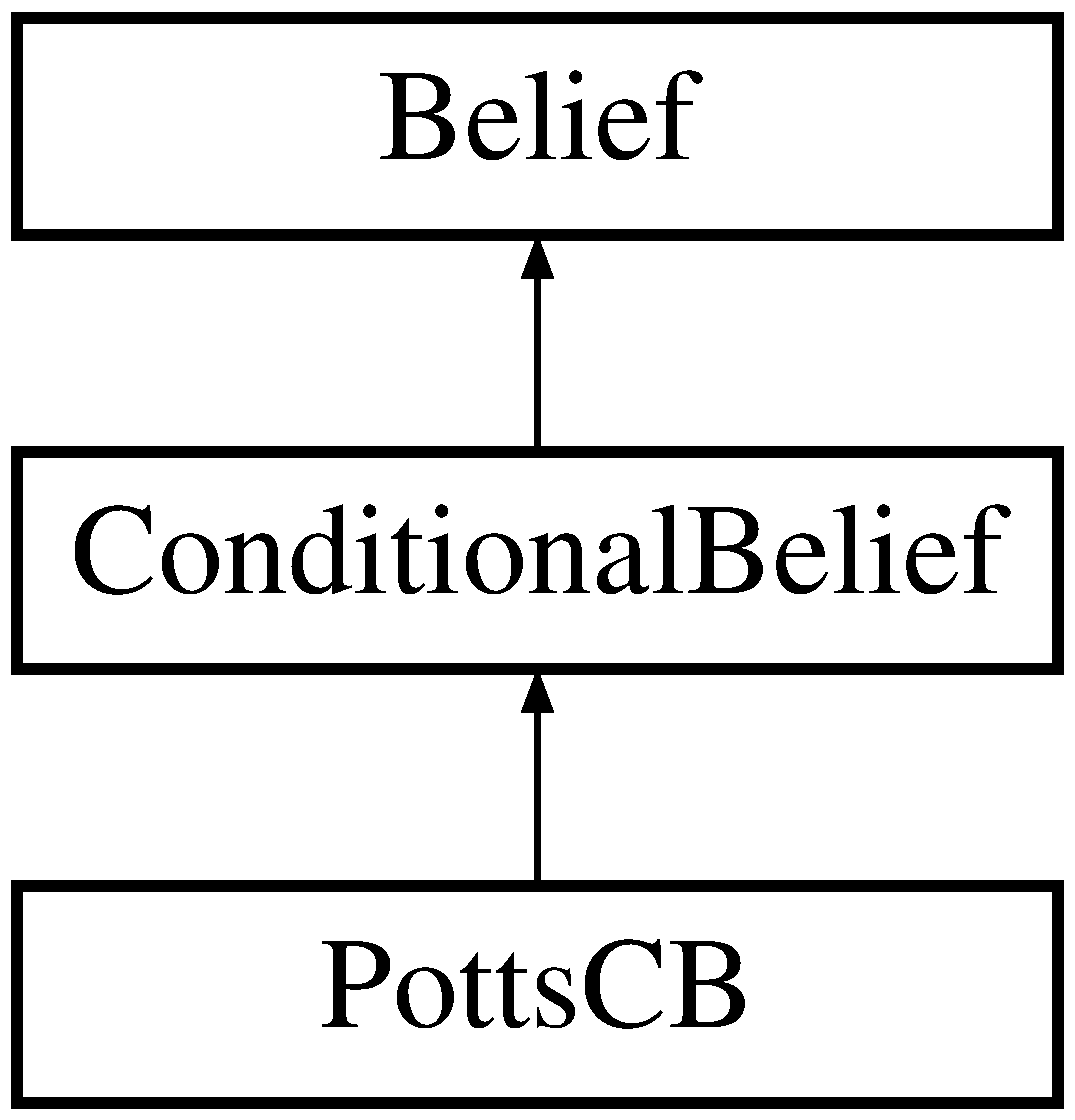
\includegraphics[height=3cm]{classBelief}
\end{center}
\end{figure}
\subsection*{Public Member Functions}
\begin{CompactItemize}
\item 
map$<$ {\bf StatePtr}, {\bf LD}, {\bf StatePtrCmp} $>$ {\bf getMp} () const
\item 
{\bf Belief} (bool intMode=false)
\begin{CompactList}\small\item\em the default constructor - note that INT\_\-MODE must be initialized before call to this \item\end{CompactList}\item 
{\bf LD} {\bf getAllocPr} () const
\begin{CompactList}\small\item\em returns the total allocated probability ( relevant to LD\_\-MODE ) \item\end{CompactList}\item 
int {\bf getTotalFreq} () const
\begin{CompactList}\small\item\em returns the totalFreq (INT\_\-MODE) \item\end{CompactList}\item 
void {\bf setPr} ({\bf StatePtr} \_\-s, {\bf LD} \_\-v=-1.0)
\item 
{\bf LD} {\bf getPr} ({\bf StatePtr} s)
\begin{CompactList}\small\item\em returns the probability of given state(if found) or BELIEF\_\-NOT\_\-FOUND=-1.0 \item\end{CompactList}\item 
{\bf $\sim$Belief} ()
\item 
void {\bf clear} ()
\item 
void {\bf normalize} ()
\begin{CompactList}\small\item\em normalizes allocPr = 1.0 \item\end{CompactList}\end{CompactItemize}
\subsection*{Public Attributes}
\begin{CompactItemize}
\item 
bool {\bf INT\_\-MODE}
\begin{CompactList}\small\item\em variable that is true when the map stores the frequency \item\end{CompactList}\end{CompactItemize}
\subsection*{Private Member Functions}
\begin{CompactItemize}
\item 
void {\bf incrTot} ()
\end{CompactItemize}
\subsection*{Private Attributes}
\begin{CompactItemize}
\item 
{\bf LD} {\bf allocPr}
\begin{CompactList}\small\item\em the total probability mass allocated in bMp \item\end{CompactList}\item 
map$<$ {\bf StatePtr}, {\bf LD}, {\bf StatePtrCmp} $>$ {\bf bMp}
\begin{CompactList}\small\item\em map having actual belief - probability pairs \item\end{CompactList}\item 
int {\bf totalFreq}
\begin{CompactList}\small\item\em variable used in tracking true\_\-pr = act\_\-pr/totalFreq ( to make compatible with int mode ) \item\end{CompactList}\end{CompactItemize}
\subsection*{Friends}
\begin{CompactItemize}
\item 
ostream \& {\bf operator$<$$<$} (ostream \&os, {\bf Belief} \&b)
\end{CompactItemize}


\subsection{Detailed Description}
class that stores all possible the beliefs 



\subsection{Constructor \& Destructor Documentation}
\index{Belief@{Belief}!Belief@{Belief}}
\index{Belief@{Belief}!Belief@{Belief}}
\subsubsection{\setlength{\rightskip}{0pt plus 5cm}Belief::Belief (bool {\em intMode} = {\tt false})\hspace{0.3cm}{\tt  [inline]}}\label{classBelief_c033cf6a5790319d7ecf3a864e61b209}


the default constructor - note that INT\_\-MODE must be initialized before call to this 

\index{Belief@{Belief}!~Belief@{$\sim$Belief}}
\index{~Belief@{$\sim$Belief}!Belief@{Belief}}
\subsubsection{\setlength{\rightskip}{0pt plus 5cm}Belief::$\sim$Belief ()\hspace{0.3cm}{\tt  [inline]}}\label{classBelief_3225e0dd40b0b2a73dd72c75c1a3acec}




\subsection{Member Function Documentation}
\index{Belief@{Belief}!incrTot@{incrTot}}
\index{incrTot@{incrTot}!Belief@{Belief}}
\subsubsection{\setlength{\rightskip}{0pt plus 5cm}void Belief::incrTot ()\hspace{0.3cm}{\tt  [inline, private]}}\label{classBelief_4cbd767671325fa2dbc951e03a5a5f5e}


\index{Belief@{Belief}!getMp@{getMp}}
\index{getMp@{getMp}!Belief@{Belief}}
\subsubsection{\setlength{\rightskip}{0pt plus 5cm}map$<${\bf StatePtr}, {\bf LD}, {\bf StatePtrCmp}$>$ Belief::getMp () const\hspace{0.3cm}{\tt  [inline]}}\label{classBelief_8ef06d897864474bf4ec7045db27bde1}


\index{Belief@{Belief}!getAllocPr@{getAllocPr}}
\index{getAllocPr@{getAllocPr}!Belief@{Belief}}
\subsubsection{\setlength{\rightskip}{0pt plus 5cm}{\bf LD} Belief::getAllocPr () const\hspace{0.3cm}{\tt  [inline]}}\label{classBelief_bc7840cece7baa070c4c9dc1e65f1951}


returns the total allocated probability ( relevant to LD\_\-MODE ) 

\index{Belief@{Belief}!getTotalFreq@{getTotalFreq}}
\index{getTotalFreq@{getTotalFreq}!Belief@{Belief}}
\subsubsection{\setlength{\rightskip}{0pt plus 5cm}int Belief::getTotalFreq () const\hspace{0.3cm}{\tt  [inline]}}\label{classBelief_24f6916c0e74d448ee2176f53c267e95}


returns the totalFreq (INT\_\-MODE) 

\index{Belief@{Belief}!setPr@{setPr}}
\index{setPr@{setPr}!Belief@{Belief}}
\subsubsection{\setlength{\rightskip}{0pt plus 5cm}void Belief::setPr ({\bf StatePtr} {\em \_\-s}, {\bf LD} {\em \_\-v} = {\tt -1.0})}\label{classBelief_56babf3f9c5c646e99b9285e749122d6}


sets the probability of given state ( if INT\_\-MODE = false) increments the frequency of given state and the totalFreqency ( if INT\_\-MODE = true ) \index{Belief@{Belief}!getPr@{getPr}}
\index{getPr@{getPr}!Belief@{Belief}}
\subsubsection{\setlength{\rightskip}{0pt plus 5cm}{\bf LD} Belief::getPr ({\bf StatePtr} {\em s})}\label{classBelief_a08084d7263223dac3192fc82a266f40}


returns the probability of given state(if found) or BELIEF\_\-NOT\_\-FOUND=-1.0 

\index{Belief@{Belief}!clear@{clear}}
\index{clear@{clear}!Belief@{Belief}}
\subsubsection{\setlength{\rightskip}{0pt plus 5cm}void Belief::clear ()\hspace{0.3cm}{\tt  [inline]}}\label{classBelief_5447bc76328b28b4c0683262fc70911e}




Reimplemented in {\bf ConditionalBelief} \doxyref{}{p.}{classConditionalBelief_c1323d280c05b3b6a245c0871d419abf}.\index{Belief@{Belief}!normalize@{normalize}}
\index{normalize@{normalize}!Belief@{Belief}}
\subsubsection{\setlength{\rightskip}{0pt plus 5cm}void Belief::normalize ()\hspace{0.3cm}{\tt  [inline]}}\label{classBelief_1fd13460b138d51f6c9f3f51962e1b41}


normalizes allocPr = 1.0 



\subsection{Friends And Related Function Documentation}
\index{Belief@{Belief}!operator<<@{operator$<$$<$}}
\index{operator<<@{operator$<$$<$}!Belief@{Belief}}
\subsubsection{\setlength{\rightskip}{0pt plus 5cm}ostream\& operator$<$$<$ (ostream \& {\em os}, {\bf Belief} \& {\em b})\hspace{0.3cm}{\tt  [friend]}}\label{classBelief_14833d2c0ad7d660d4a5c50902b1f2c3}




\subsection{Member Data Documentation}
\index{Belief@{Belief}!allocPr@{allocPr}}
\index{allocPr@{allocPr}!Belief@{Belief}}
\subsubsection{\setlength{\rightskip}{0pt plus 5cm}{\bf LD} {\bf Belief::allocPr}\hspace{0.3cm}{\tt  [private]}}\label{classBelief_13c38fd093ebb4af5bc6b0bc866168b4}


the total probability mass allocated in bMp 

\index{Belief@{Belief}!bMp@{bMp}}
\index{bMp@{bMp}!Belief@{Belief}}
\subsubsection{\setlength{\rightskip}{0pt plus 5cm}map$<${\bf StatePtr}, {\bf LD}, {\bf StatePtrCmp}$>$ {\bf Belief::bMp}\hspace{0.3cm}{\tt  [private]}}\label{classBelief_725e30c32b2cfd41876879af192a953b}


map having actual belief - probability pairs 

\index{Belief@{Belief}!totalFreq@{totalFreq}}
\index{totalFreq@{totalFreq}!Belief@{Belief}}
\subsubsection{\setlength{\rightskip}{0pt plus 5cm}int {\bf Belief::totalFreq}\hspace{0.3cm}{\tt  [private]}}\label{classBelief_294ec0bdb705e01393c1d4beb9856666}


variable used in tracking true\_\-pr = act\_\-pr/totalFreq ( to make compatible with int mode ) 

\index{Belief@{Belief}!INT_MODE@{INT\_\-MODE}}
\index{INT_MODE@{INT\_\-MODE}!Belief@{Belief}}
\subsubsection{\setlength{\rightskip}{0pt plus 5cm}bool {\bf Belief::INT\_\-MODE}}\label{classBelief_e4ec5bb27d2de6952fabb843671d3340}


variable that is true when the map stores the frequency 



The documentation for this class was generated from the following files:\begin{CompactItemize}
\item 
inc/{\bf belief.h}\item 
src/{\bf belief.cpp}\end{CompactItemize}

\section{BPGraph Class Reference}
\label{classBPGraph}\index{BPGraph@{BPGraph}}
{\tt \#include $<$bpgraph.h$>$}



The documentation for this class was generated from the following file:\begin{CompactItemize}
\item 
inc/{\bf bpgraph.h}\end{CompactItemize}

\section{Cluster Struct Reference}
\label{structCluster}\index{Cluster@{Cluster}}
{\tt \#include $<$main.h$>$}

\subsection*{Public Member Functions}
\begin{CompactItemize}
\item 
{\bf Cluster} (vector$<$ string $>$ vars, vector$<$ string $>$ fctrs)
\item 
{\bf Cluster} ()
\item 
bool {\bf operator==} (const {\bf Cluster} \&c) const 
\item 
string {\bf getRegionId} () const
\item 
bool {\bf operator!=} (const {\bf Cluster} \&c) const 
\end{CompactItemize}
\subsection*{Static Public Member Functions}
\begin{CompactItemize}
\item 
static bool {\bf subset} (const {\bf Cluster} \&c1, const {\bf Cluster} \&c2)
\begin{CompactList}\small\item\em returns c1 subset c2 \item\end{CompactList}\item 
static bool {\bf intersection} ({\bf Cluster} $\ast$cc, const {\bf Cluster} \&c1, const {\bf Cluster} \&c2)
\end{CompactItemize}
\subsection*{Public Attributes}
\begin{CompactItemize}
\item 
vector$<$ string $>$ {\bf first}
\item 
vector$<$ string $>$ {\bf second}
\end{CompactItemize}
\subsection*{Friends}
\begin{CompactItemize}
\item 
ostream \& {\bf operator$<$$<$} (ostream \&os, const {\bf Cluster} \&c)
\end{CompactItemize}


\subsection{Constructor \& Destructor Documentation}
\index{Cluster@{Cluster}!Cluster@{Cluster}}
\index{Cluster@{Cluster}!Cluster@{Cluster}}
\subsubsection{\setlength{\rightskip}{0pt plus 5cm}Cluster::Cluster (vector$<$ string $>$ {\em vars}, vector$<$ string $>$ {\em fctrs})\hspace{0.3cm}{\tt  [inline]}}\label{structCluster_2a24a407dd0ed35b92ba5a152bc908a0}


\index{Cluster@{Cluster}!Cluster@{Cluster}}
\index{Cluster@{Cluster}!Cluster@{Cluster}}
\subsubsection{\setlength{\rightskip}{0pt plus 5cm}Cluster::Cluster ()\hspace{0.3cm}{\tt  [inline]}}\label{structCluster_bf2af19044d4b84b9c9eb4f723453139}




\subsection{Member Function Documentation}
\index{Cluster@{Cluster}!subset@{subset}}
\index{subset@{subset}!Cluster@{Cluster}}
\subsubsection{\setlength{\rightskip}{0pt plus 5cm}bool Cluster::subset (const {\bf Cluster} \& {\em c1}, const {\bf Cluster} \& {\em c2})\hspace{0.3cm}{\tt  [static]}}\label{structCluster_7b0d5c799fcd34dfeda18800f73b340e}


returns c1 subset c2 

\index{Cluster@{Cluster}!operator==@{operator==}}
\index{operator==@{operator==}!Cluster@{Cluster}}
\subsubsection{\setlength{\rightskip}{0pt plus 5cm}bool Cluster::operator== (const {\bf Cluster} \& {\em c}) const\hspace{0.3cm}{\tt  [inline]}}\label{structCluster_2daa42739b49a758a8f0a7865e4d213e}


\index{Cluster@{Cluster}!getRegionId@{getRegionId}}
\index{getRegionId@{getRegionId}!Cluster@{Cluster}}
\subsubsection{\setlength{\rightskip}{0pt plus 5cm}string Cluster::getRegionId () const\hspace{0.3cm}{\tt  [inline]}}\label{structCluster_bbaa46277d1fa6e3c7e1a3b240d723ce}


\index{Cluster@{Cluster}!operator"!=@{operator"!=}}
\index{operator"!=@{operator"!=}!Cluster@{Cluster}}
\subsubsection{\setlength{\rightskip}{0pt plus 5cm}bool Cluster::operator!= (const {\bf Cluster} \& {\em c}) const\hspace{0.3cm}{\tt  [inline]}}\label{structCluster_fa0ee61e750a324e1541eb8748b5b21b}


\index{Cluster@{Cluster}!intersection@{intersection}}
\index{intersection@{intersection}!Cluster@{Cluster}}
\subsubsection{\setlength{\rightskip}{0pt plus 5cm}bool Cluster::intersection ({\bf Cluster} $\ast$ {\em cc}, const {\bf Cluster} \& {\em c1}, const {\bf Cluster} \& {\em c2})\hspace{0.3cm}{\tt  [static]}}\label{structCluster_9a4d09cf7d1a6ebd437b42ad6983f00b}




\subsection{Friends And Related Function Documentation}
\index{Cluster@{Cluster}!operator<<@{operator$<$$<$}}
\index{operator<<@{operator$<$$<$}!Cluster@{Cluster}}
\subsubsection{\setlength{\rightskip}{0pt plus 5cm}ostream\& operator$<$$<$ (ostream \& {\em os}, const {\bf Cluster} \& {\em c})\hspace{0.3cm}{\tt  [friend]}}\label{structCluster_66e4ab0733f65907e1cb0a41f9c11360}




\subsection{Member Data Documentation}
\index{Cluster@{Cluster}!first@{first}}
\index{first@{first}!Cluster@{Cluster}}
\subsubsection{\setlength{\rightskip}{0pt plus 5cm}vector$<$string$>$ {\bf Cluster::first}}\label{structCluster_6faa4a8072fabb9df52bc5882ad83d28}


\index{Cluster@{Cluster}!second@{second}}
\index{second@{second}!Cluster@{Cluster}}
\subsubsection{\setlength{\rightskip}{0pt plus 5cm}vector$<$string$>$ {\bf Cluster::second}}\label{structCluster_defe091a0a3e6834c3b858f9eb23d2c2}




The documentation for this struct was generated from the following files:\begin{CompactItemize}
\item 
inc/{\bf main.h}\item 
src/{\bf main.cpp}\end{CompactItemize}

\section{ClusterCmp Struct Reference}
\label{structClusterCmp}\index{ClusterCmp@{ClusterCmp}}
{\tt \#include $<$main.h$>$}

\subsection*{Public Member Functions}
\begin{CompactItemize}
\item 
bool {\bf operator()} (const {\bf Cluster} \&c1, const {\bf Cluster} \&c2) const
\end{CompactItemize}


\subsection{Member Function Documentation}
\index{ClusterCmp@{ClusterCmp}!operator()@{operator()}}
\index{operator()@{operator()}!ClusterCmp@{ClusterCmp}}
\subsubsection{\setlength{\rightskip}{0pt plus 5cm}bool ClusterCmp::operator() (const {\bf Cluster} \& {\em c1}, const {\bf Cluster} \& {\em c2}) const\hspace{0.3cm}{\tt  [inline]}}\label{structClusterCmp_ebf1bbed30dee33111a745a469dbb474}




The documentation for this struct was generated from the following file:\begin{CompactItemize}
\item 
inc/{\bf main.h}\end{CompactItemize}

\section{ConditionalBelief Class Reference}
\label{classConditionalBelief}\index{ConditionalBelief@{ConditionalBelief}}
class that stores the conditional beliefs  


{\tt \#include $<$belief.h$>$}

Inheritance diagram for ConditionalBelief::\begin{figure}[H]
\begin{center}
\leavevmode
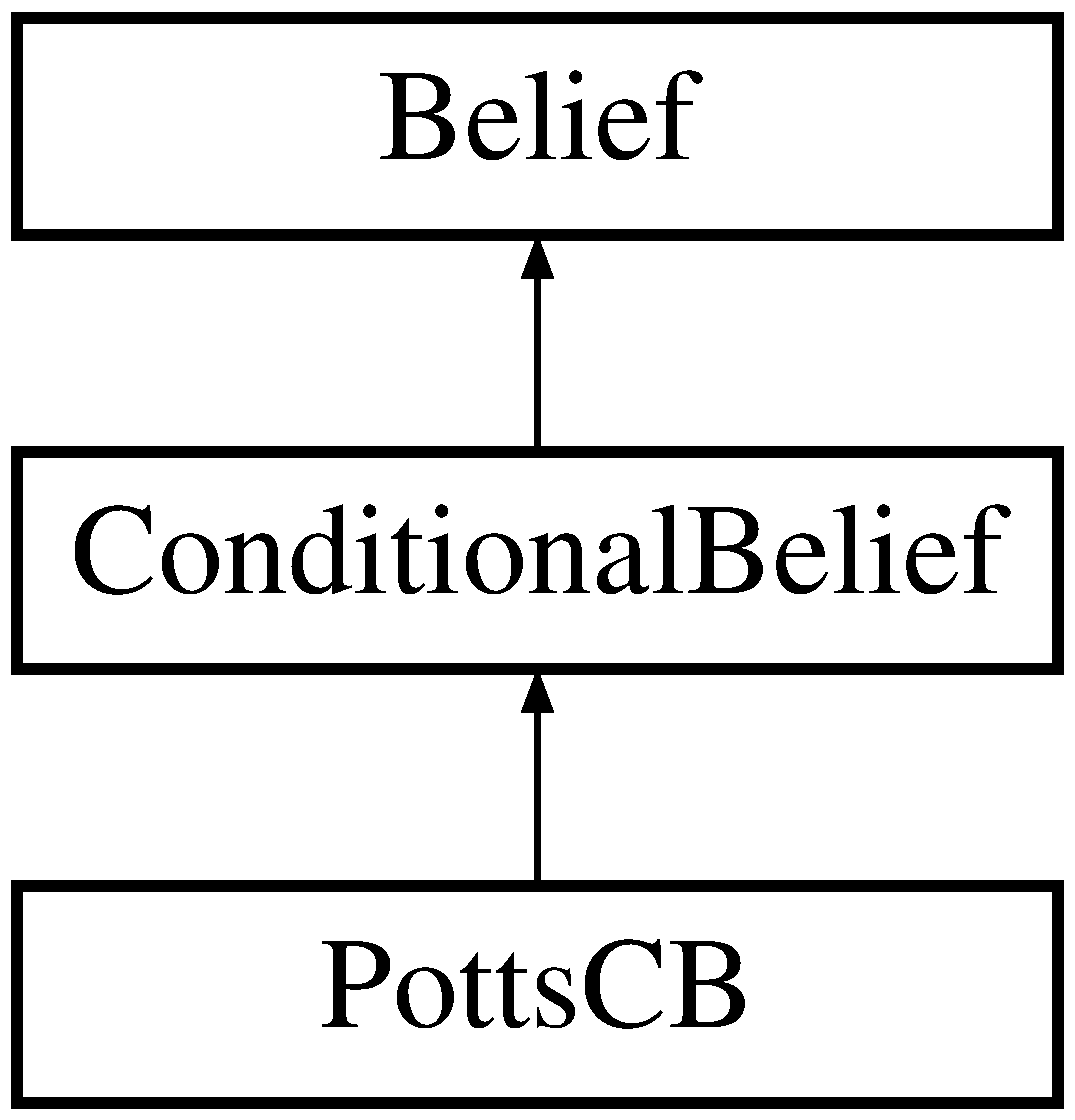
\includegraphics[height=3cm]{classConditionalBelief}
\end{center}
\end{figure}
\subsection*{Public Member Functions}
\begin{CompactItemize}
\item 
void {\bf clear} ()
\item 
std::map$<$ {\bf StatePtr}, {\bf Belief}, {\bf StatePtrCmp} $>$ $\ast$ {\bf getCbMpPtr} ()
\item 
{\bf BeliefPtr} {\bf getBeliefForState} ({\bf StatePtr} sptr)
\item 
void {\bf setPr} ({\bf StatePtr} sC, {\bf StatePtr} sN, {\bf LD} \_\-cbp, {\bf LD} \_\-origp=-1.0)
\item 
{\bf LD} {\bf getPr} ({\bf StatePtr} sC, {\bf StatePtr} sN)
\begin{CompactList}\small\item\em returns the probability p(sN $|$ sC) or BELIEF\_\-NOT\_\-FOUND \item\end{CompactList}\item 
{\bf LD} {\bf getAllocPr} ({\bf StatePtr} sC)
\begin{CompactList}\small\item\em get the allocation corresponding to belief starting at sC or BELIEF\_\-NOT\_\-FOUND \item\end{CompactList}\item 
{\bf LD} {\bf getTotalAlloc} ()
\begin{CompactList}\small\item\em the total allocatio present \item\end{CompactList}\end{CompactItemize}
\subsection*{Private Attributes}
\begin{CompactItemize}
\item 
std::map$<$ {\bf StatePtr}, {\bf Belief}, {\bf StatePtrCmp} $>$ {\bf cbMp}
\end{CompactItemize}
\subsection*{Friends}
\begin{CompactItemize}
\item 
ostream \& {\bf operator$<$$<$} (ostream \&os, {\bf ConditionalBelief} \&b)
\end{CompactItemize}


\subsection{Detailed Description}
class that stores the conditional beliefs 



\subsection{Member Function Documentation}
\index{ConditionalBelief@{ConditionalBelief}!clear@{clear}}
\index{clear@{clear}!ConditionalBelief@{ConditionalBelief}}
\subsubsection{\setlength{\rightskip}{0pt plus 5cm}void ConditionalBelief::clear ()\hspace{0.3cm}{\tt  [inline]}}\label{classConditionalBelief_c1323d280c05b3b6a245c0871d419abf}




Reimplemented from {\bf Belief} \doxyref{}{p.}{classBelief_5447bc76328b28b4c0683262fc70911e}.\index{ConditionalBelief@{ConditionalBelief}!getCbMpPtr@{getCbMpPtr}}
\index{getCbMpPtr@{getCbMpPtr}!ConditionalBelief@{ConditionalBelief}}
\subsubsection{\setlength{\rightskip}{0pt plus 5cm}std::map$<${\bf StatePtr}, {\bf Belief}, {\bf StatePtrCmp}$>$$\ast$ ConditionalBelief::getCbMpPtr ()\hspace{0.3cm}{\tt  [inline]}}\label{classConditionalBelief_098347b1d8147ff8ce889eed434d8499}


\index{ConditionalBelief@{ConditionalBelief}!getBeliefForState@{getBeliefForState}}
\index{getBeliefForState@{getBeliefForState}!ConditionalBelief@{ConditionalBelief}}
\subsubsection{\setlength{\rightskip}{0pt plus 5cm}{\bf BeliefPtr} ConditionalBelief::getBeliefForState ({\bf StatePtr} {\em sptr})\hspace{0.3cm}{\tt  [inline]}}\label{classConditionalBelief_87dd91c7f764927069d4ba4328d3ae4d}


\index{ConditionalBelief@{ConditionalBelief}!setPr@{setPr}}
\index{setPr@{setPr}!ConditionalBelief@{ConditionalBelief}}
\subsubsection{\setlength{\rightskip}{0pt plus 5cm}void ConditionalBelief::setPr ({\bf StatePtr} {\em sC}, {\bf StatePtr} {\em sN}, {\bf LD} {\em \_\-cbp}, {\bf LD} {\em \_\-origp} = {\tt -1.0})}\label{classConditionalBelief_d4074569aedf433c0b829cbd6ff68835}


sets the probability of finding P(next state $|$ current state) P(sN $|$ sC) = \_\-cbp P(sC) = \_\-origp \index{ConditionalBelief@{ConditionalBelief}!getPr@{getPr}}
\index{getPr@{getPr}!ConditionalBelief@{ConditionalBelief}}
\subsubsection{\setlength{\rightskip}{0pt plus 5cm}{\bf LD} ConditionalBelief::getPr ({\bf StatePtr} {\em sC}, {\bf StatePtr} {\em sN})}\label{classConditionalBelief_66ced9bc695d3503e06a02ca95207a21}


returns the probability p(sN $|$ sC) or BELIEF\_\-NOT\_\-FOUND 



Reimplemented in {\bf PottsCB} \doxyref{}{p.}{classPottsCB_cac254c4f74d94caa1ba23343e01b96b}.\index{ConditionalBelief@{ConditionalBelief}!getAllocPr@{getAllocPr}}
\index{getAllocPr@{getAllocPr}!ConditionalBelief@{ConditionalBelief}}
\subsubsection{\setlength{\rightskip}{0pt plus 5cm}{\bf LD} ConditionalBelief::getAllocPr ({\bf StatePtr} {\em sC})}\label{classConditionalBelief_c041ff20cbd4925228d6901b0d71cc99}


get the allocation corresponding to belief starting at sC or BELIEF\_\-NOT\_\-FOUND 

\index{ConditionalBelief@{ConditionalBelief}!getTotalAlloc@{getTotalAlloc}}
\index{getTotalAlloc@{getTotalAlloc}!ConditionalBelief@{ConditionalBelief}}
\subsubsection{\setlength{\rightskip}{0pt plus 5cm}{\bf LD} ConditionalBelief::getTotalAlloc ()}\label{classConditionalBelief_87033ffe78b6ac8f6a2ca498b30a1c54}


the total allocatio present 



\subsection{Friends And Related Function Documentation}
\index{ConditionalBelief@{ConditionalBelief}!operator<<@{operator$<$$<$}}
\index{operator<<@{operator$<$$<$}!ConditionalBelief@{ConditionalBelief}}
\subsubsection{\setlength{\rightskip}{0pt plus 5cm}ostream\& operator$<$$<$ (ostream \& {\em os}, {\bf ConditionalBelief} \& {\em b})\hspace{0.3cm}{\tt  [friend]}}\label{classConditionalBelief_b1ba4b45412665954a8fc0df4bad8c1f}




\subsection{Member Data Documentation}
\index{ConditionalBelief@{ConditionalBelief}!cbMp@{cbMp}}
\index{cbMp@{cbMp}!ConditionalBelief@{ConditionalBelief}}
\subsubsection{\setlength{\rightskip}{0pt plus 5cm}std::map$<${\bf StatePtr}, {\bf Belief}, {\bf StatePtrCmp}$>$ {\bf ConditionalBelief::cbMp}\hspace{0.3cm}{\tt  [private]}}\label{classConditionalBelief_f447de6620faf8c62a0bdb8224507b83}




The documentation for this class was generated from the following files:\begin{CompactItemize}
\item 
inc/{\bf belief.h}\item 
src/{\bf belief.cpp}\end{CompactItemize}

\section{DynNode Class Reference}
\label{classDynNode}\index{DynNode@{DynNode}}
node having conditional forward time belief information  


{\tt \#include $<$node.h$>$}

Inheritance diagram for DynNode::\begin{figure}[H]
\begin{center}
\leavevmode
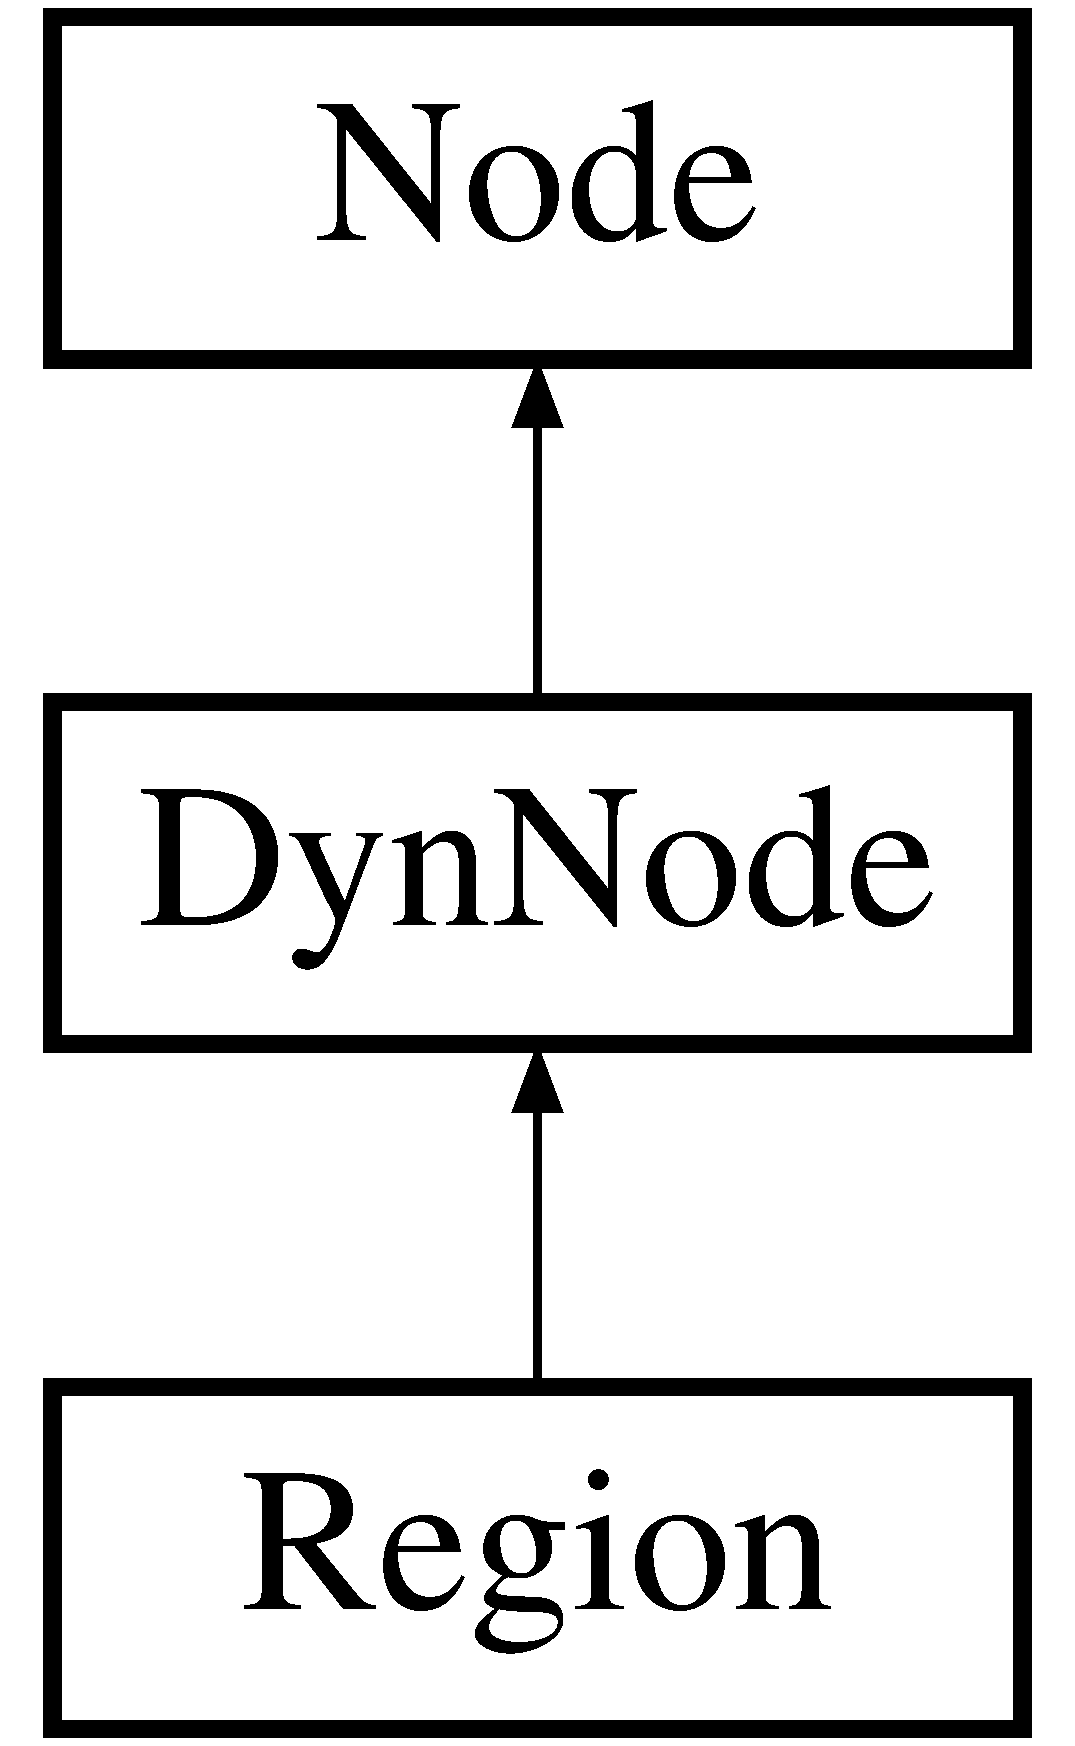
\includegraphics[height=3cm]{classDynNode}
\end{center}
\end{figure}
\subsection*{Public Member Functions}
\begin{CompactItemize}
\item 
{\bf DynNode} ()
\item 
void {\bf setConditionalBelief} ({\bf ConditionalBelief} $\ast$c)
\item 
{\bf DynNode} (string s, int {\bf numVar}, {\bf Belief} $\ast$bp=0, {\bf ConditionalBelief} $\ast$cbp=0, int \_\-type=-1)
\item 
{\bf ConditionalBelief} $\ast$ {\bf getConditionalBeliefPtr} ()
\item 
{\bf $\sim$DynNode} ()
\end{CompactItemize}
\subsection*{Private Attributes}
\begin{CompactItemize}
\item 
{\bf ConditionalBelief} $\ast$ {\bf cPtr}
\begin{CompactList}\small\item\em set of conditional beliefs about next state given current state \item\end{CompactList}\end{CompactItemize}
\subsection*{Friends}
\begin{CompactItemize}
\item 
ostream \& {\bf operator$<$$<$} (ostream \&os, {\bf DynNode} \&dn)
\end{CompactItemize}


\subsection{Detailed Description}
node having conditional forward time belief information 



\subsection{Constructor \& Destructor Documentation}
\index{DynNode@{DynNode}!DynNode@{DynNode}}
\index{DynNode@{DynNode}!DynNode@{DynNode}}
\subsubsection{\setlength{\rightskip}{0pt plus 5cm}DynNode::DynNode ()\hspace{0.3cm}{\tt  [inline]}}\label{classDynNode_f6e18d6646c290d1cc617e7f97837607}


\index{DynNode@{DynNode}!DynNode@{DynNode}}
\index{DynNode@{DynNode}!DynNode@{DynNode}}
\subsubsection{\setlength{\rightskip}{0pt plus 5cm}DynNode::DynNode (string {\em s}, int {\em numVar}, {\bf Belief} $\ast$ {\em bp} = {\tt 0}, {\bf ConditionalBelief} $\ast$ {\em cbp} = {\tt 0}, int {\em \_\-type} = {\tt -1})}\label{classDynNode_06541a46e4f4fc4db612917774e02a85}


\index{DynNode@{DynNode}!~DynNode@{$\sim$DynNode}}
\index{~DynNode@{$\sim$DynNode}!DynNode@{DynNode}}
\subsubsection{\setlength{\rightskip}{0pt plus 5cm}DynNode::$\sim$DynNode ()\hspace{0.3cm}{\tt  [inline]}}\label{classDynNode_be9a7aa589d8a07b52449724a9ca6240}




\subsection{Member Function Documentation}
\index{DynNode@{DynNode}!setConditionalBelief@{setConditionalBelief}}
\index{setConditionalBelief@{setConditionalBelief}!DynNode@{DynNode}}
\subsubsection{\setlength{\rightskip}{0pt plus 5cm}void DynNode::setConditionalBelief ({\bf ConditionalBelief} $\ast$ {\em c})\hspace{0.3cm}{\tt  [inline]}}\label{classDynNode_902d5999f06d232efba16c77b7366809}


\index{DynNode@{DynNode}!getConditionalBeliefPtr@{getConditionalBeliefPtr}}
\index{getConditionalBeliefPtr@{getConditionalBeliefPtr}!DynNode@{DynNode}}
\subsubsection{\setlength{\rightskip}{0pt plus 5cm}{\bf ConditionalBelief}$\ast$ DynNode::getConditionalBeliefPtr ()\hspace{0.3cm}{\tt  [inline]}}\label{classDynNode_adf2e00588988f9705de42c4c2930918}




\subsection{Friends And Related Function Documentation}
\index{DynNode@{DynNode}!operator<<@{operator$<$$<$}}
\index{operator<<@{operator$<$$<$}!DynNode@{DynNode}}
\subsubsection{\setlength{\rightskip}{0pt plus 5cm}ostream\& operator$<$$<$ (ostream \& {\em os}, {\bf DynNode} \& {\em dn})\hspace{0.3cm}{\tt  [friend]}}\label{classDynNode_ce217a788f52579d20aeabc6ef30650e}




\subsection{Member Data Documentation}
\index{DynNode@{DynNode}!cPtr@{cPtr}}
\index{cPtr@{cPtr}!DynNode@{DynNode}}
\subsubsection{\setlength{\rightskip}{0pt plus 5cm}{\bf ConditionalBelief}$\ast$ {\bf DynNode::cPtr}\hspace{0.3cm}{\tt  [private]}}\label{classDynNode_03326c806301531f149a01c9291245a9}


set of conditional beliefs about next state given current state 



The documentation for this class was generated from the following files:\begin{CompactItemize}
\item 
inc/{\bf node.h}\item 
src/{\bf node.cpp}\end{CompactItemize}

\section{EdgeList Class Reference}
\label{classEdgeList}\index{EdgeList@{EdgeList}}
{\tt \#include $<$myedge.h$>$}

\subsection*{Public Member Functions}
\begin{CompactItemize}
\item 
{\bf EdgeList} ()
\item 
void {\bf addEdge} ({\bf MyEdge} e)
\item 
int {\bf getSize} ()
\item 
vector$<$ {\bf MyEdge} $>$::iterator {\bf begin} ()
\item 
vector$<$ {\bf MyEdge} $>$::iterator {\bf end} ()
\end{CompactItemize}
\subsection*{Private Attributes}
\begin{CompactItemize}
\item 
vector$<$ {\bf MyEdge} $>$ {\bf edgeList}
\end{CompactItemize}


\subsection{Constructor \& Destructor Documentation}
\index{EdgeList@{EdgeList}!EdgeList@{EdgeList}}
\index{EdgeList@{EdgeList}!EdgeList@{EdgeList}}
\subsubsection{\setlength{\rightskip}{0pt plus 5cm}EdgeList::EdgeList ()}\label{classEdgeList_ae4da15044dbea245b4b3b7f2876b3f6}




\subsection{Member Function Documentation}
\index{EdgeList@{EdgeList}!addEdge@{addEdge}}
\index{addEdge@{addEdge}!EdgeList@{EdgeList}}
\subsubsection{\setlength{\rightskip}{0pt plus 5cm}void EdgeList::addEdge ({\bf MyEdge} {\em e})\hspace{0.3cm}{\tt  [inline]}}\label{classEdgeList_fb734ef2756a8c48cd9a89111580091a}


\index{EdgeList@{EdgeList}!getSize@{getSize}}
\index{getSize@{getSize}!EdgeList@{EdgeList}}
\subsubsection{\setlength{\rightskip}{0pt plus 5cm}int EdgeList::getSize ()\hspace{0.3cm}{\tt  [inline]}}\label{classEdgeList_f9abf777950110154da92cdf0c44cc1a}


\index{EdgeList@{EdgeList}!begin@{begin}}
\index{begin@{begin}!EdgeList@{EdgeList}}
\subsubsection{\setlength{\rightskip}{0pt plus 5cm}vector$<${\bf MyEdge}$>$::iterator EdgeList::begin ()\hspace{0.3cm}{\tt  [inline]}}\label{classEdgeList_a1c1228a6afaf8d89a42ee82b1e977cd}


\index{EdgeList@{EdgeList}!end@{end}}
\index{end@{end}!EdgeList@{EdgeList}}
\subsubsection{\setlength{\rightskip}{0pt plus 5cm}vector$<${\bf MyEdge}$>$::iterator EdgeList::end ()\hspace{0.3cm}{\tt  [inline]}}\label{classEdgeList_f0e89346b62e539d638a8656780bfeee}




\subsection{Member Data Documentation}
\index{EdgeList@{EdgeList}!edgeList@{edgeList}}
\index{edgeList@{edgeList}!EdgeList@{EdgeList}}
\subsubsection{\setlength{\rightskip}{0pt plus 5cm}vector$<${\bf MyEdge}$>$ {\bf EdgeList::edgeList}\hspace{0.3cm}{\tt  [private]}}\label{classEdgeList_22d4d9791737cdb8d0c44476e572c622}




The documentation for this class was generated from the following file:\begin{CompactItemize}
\item 
inc/{\bf myedge.h}\end{CompactItemize}

\section{EdgeProperty Struct Reference}
\label{structEdgeProperty}\index{EdgeProperty@{EdgeProperty}}
{\tt \#include $<$EdgeProperty.h$>$}

\subsection*{Public Attributes}
\begin{CompactItemize}
\item 
double {\bf msg} [2]
\end{CompactItemize}


\subsection{Member Data Documentation}
\index{EdgeProperty@{EdgeProperty}!msg@{msg}}
\index{msg@{msg}!EdgeProperty@{EdgeProperty}}
\subsubsection{\setlength{\rightskip}{0pt plus 5cm}double {\bf EdgeProperty::msg}[2]}\label{structEdgeProperty_07dfcb88013debef49aa1aaf6bcba611}




The documentation for this struct was generated from the following file:\begin{CompactItemize}
\item 
inc/{\bf EdgeProperty.h}\end{CompactItemize}

\section{FactorGraph Class Reference}
\label{classFactorGraph}\index{FactorGraph@{FactorGraph}}
{\tt \#include $<$mygraph.h$>$}

Inheritance diagram for FactorGraph::\begin{figure}[H]
\begin{center}
\leavevmode
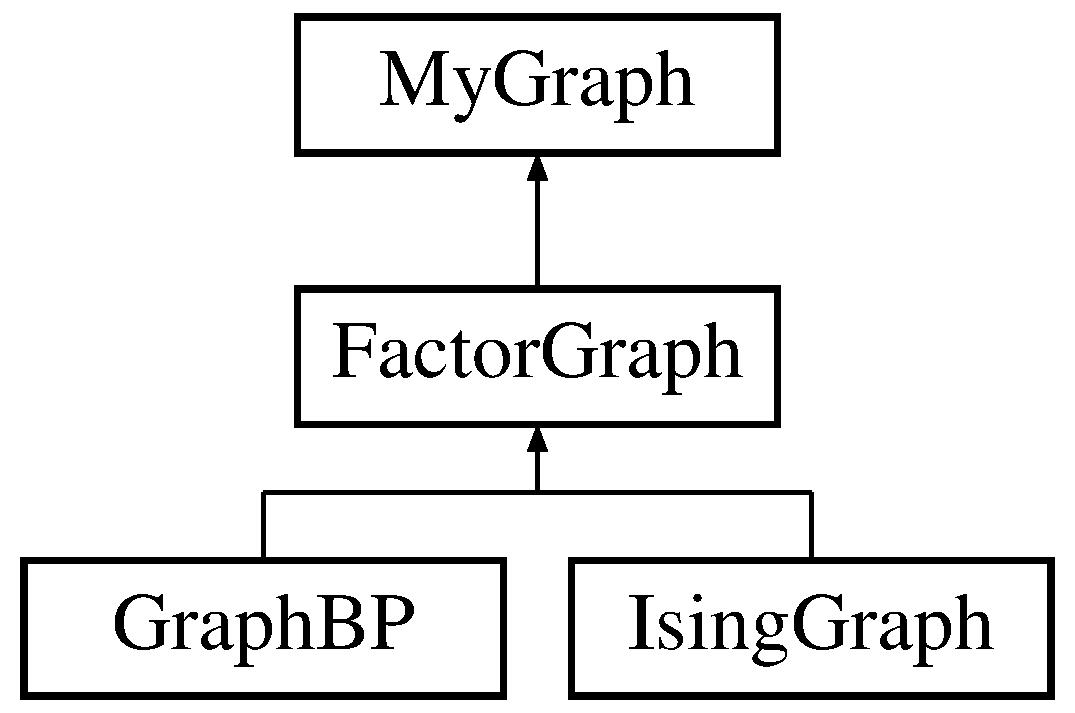
\includegraphics[height=3cm]{classFactorGraph}
\end{center}
\end{figure}
\subsection*{Public Member Functions}
\begin{CompactItemize}
\item 
bool {\bf bp\_\-iter} (bool ch)
\item 
int {\bf getStPtrIdx} ({\bf StatePtr} sp)
\item 
{\bf FactorGraph} ()
\item 
{\bf LD} {\bf getTrueZ} ()
\item 
{\bf LD} {\bf getTrueP} ({\bf StatePtr} s)
\item 
{\bf StatePtr} {\bf getFactorStatePtr} ({\bf StatePtr} sComplete, string fctrNodeId)
\item 
bool {\bf isFactor} (const {\bf NodePtr} np)
\item 
vector$<$ {\bf INT} $>$ {\bf getIthStVec} (int i, int N, vector$<$ {\bf INT} $>$ vals)
\item 
{\bf LD} {\bf updateN} ({\bf NodePtr} np, {\bf NodePtr} nc)
\begin{CompactList}\small\item\em updates the child to parent message \item\end{CompactList}\item 
{\bf LD} {\bf updateM} ({\bf NodePtr} np, {\bf NodePtr} nc)
\begin{CompactList}\small\item\em updates the parent to child message \item\end{CompactList}\item 
void {\bf updateMN} ({\bf NodePtr} np, {\bf NodePtr} nc)
\begin{CompactList}\small\item\em updates the belief at variable \item\end{CompactList}\item 
bool {\bf updateB} ({\bf NodePtr} nv)
\begin{CompactList}\small\item\em updates the belief at variable \item\end{CompactList}\item 
pair$<$ {\bf EdgePtr}, {\bf EdgePtr} $>$ {\bf addEdge} ({\bf NodePtr} ns, {\bf NodePtr} nt, bool checkExisting=false)
\begin{CompactList}\small\item\em additionally initializes the msgMp for each edge \item\end{CompactList}\item 
void {\bf bp\_\-synch} (bool ch)
\item 
{\bf LD} {\bf getMarginalProb} (vector$<$ pair$<$ string, int $>$ $>$ VVP)
\begin{CompactList}\small\item\em computes the marginal probability for given state \item\end{CompactList}\end{CompactItemize}
\subsection*{Public Attributes}
\begin{CompactItemize}
\item 
bool {\bf dirtyF}
\item 
{\bf LD} {\bf Fapprox}
\end{CompactItemize}
\subsection*{Private Attributes}
\begin{CompactItemize}
\item 
bool {\bf dirtyZ}
\item 
{\bf LD} {\bf trueZ}
\item 
{\bf LD} {\bf theta}
\item 
map$<$ long long, {\bf LD} $>$ {\bf trueProbMp}
\end{CompactItemize}


\subsection{Detailed Description}
Graph structure corresponding to factor graphs\begin{itemize}
\item supports BP algorithm\item constrains factor node id to F\_\-(list of var\_\-ids separated by \_\-) eg, F\_\-X0.0\_\-X0.1\item constrains variable node id to X(nodeInt) eg, X0.0 \end{itemize}




\subsection{Constructor \& Destructor Documentation}
\index{FactorGraph@{FactorGraph}!FactorGraph@{FactorGraph}}
\index{FactorGraph@{FactorGraph}!FactorGraph@{FactorGraph}}
\subsubsection{\setlength{\rightskip}{0pt plus 5cm}FactorGraph::FactorGraph ()\hspace{0.3cm}{\tt  [inline]}}\label{classFactorGraph_c4072e735fd541d0c47a4783eaf5d212}




\subsection{Member Function Documentation}
\index{FactorGraph@{FactorGraph}!bp_iter@{bp\_\-iter}}
\index{bp_iter@{bp\_\-iter}!FactorGraph@{FactorGraph}}
\subsubsection{\setlength{\rightskip}{0pt plus 5cm}bool FactorGraph::bp\_\-iter (bool {\em ch})}\label{classFactorGraph_9f696a79697b96d09816a082939917a0}


\index{FactorGraph@{FactorGraph}!getStPtrIdx@{getStPtrIdx}}
\index{getStPtrIdx@{getStPtrIdx}!FactorGraph@{FactorGraph}}
\subsubsection{\setlength{\rightskip}{0pt plus 5cm}int FactorGraph::getStPtrIdx ({\bf StatePtr} {\em sp})\hspace{0.3cm}{\tt  [inline]}}\label{classFactorGraph_8664914707345bca9df900859b927e20}


\index{FactorGraph@{FactorGraph}!getTrueZ@{getTrueZ}}
\index{getTrueZ@{getTrueZ}!FactorGraph@{FactorGraph}}
\subsubsection{\setlength{\rightskip}{0pt plus 5cm}{\bf LD} FactorGraph::getTrueZ ()}\label{classFactorGraph_86259c82f067fb5a3bbce8af85da7829}


\index{FactorGraph@{FactorGraph}!getTrueP@{getTrueP}}
\index{getTrueP@{getTrueP}!FactorGraph@{FactorGraph}}
\subsubsection{\setlength{\rightskip}{0pt plus 5cm}{\bf LD} FactorGraph::getTrueP ({\bf StatePtr} {\em s})}\label{classFactorGraph_9bedbc5284f2eda9cf52debb34f8e551}


\index{FactorGraph@{FactorGraph}!getFactorStatePtr@{getFactorStatePtr}}
\index{getFactorStatePtr@{getFactorStatePtr}!FactorGraph@{FactorGraph}}
\subsubsection{\setlength{\rightskip}{0pt plus 5cm}{\bf StatePtr} FactorGraph::getFactorStatePtr ({\bf StatePtr} {\em sComplete}, string {\em fctrNodeId})}\label{classFactorGraph_9b030982969b64af589358a6b9fa6519}


\index{FactorGraph@{FactorGraph}!isFactor@{isFactor}}
\index{isFactor@{isFactor}!FactorGraph@{FactorGraph}}
\subsubsection{\setlength{\rightskip}{0pt plus 5cm}bool FactorGraph::isFactor (const {\bf NodePtr} {\em np})\hspace{0.3cm}{\tt  [inline]}}\label{classFactorGraph_b31b7ea37fd273a4ba48697de63aa506}


\index{FactorGraph@{FactorGraph}!getIthStVec@{getIthStVec}}
\index{getIthStVec@{getIthStVec}!FactorGraph@{FactorGraph}}
\subsubsection{\setlength{\rightskip}{0pt plus 5cm}vector$<$ {\bf INT} $>$ FactorGraph::getIthStVec (int {\em i}, int {\em N}, vector$<$ {\bf INT} $>$ {\em vals})}\label{classFactorGraph_88b4c31e3f3a41df1ab100d645c288f5}


\index{FactorGraph@{FactorGraph}!updateN@{updateN}}
\index{updateN@{updateN}!FactorGraph@{FactorGraph}}
\subsubsection{\setlength{\rightskip}{0pt plus 5cm}{\bf LD} FactorGraph::updateN ({\bf NodePtr} {\em np}, {\bf NodePtr} {\em nc})}\label{classFactorGraph_50fe3b70c2cf57b3ff7c885def2d0119}


updates the child to parent message 



Reimplemented in {\bf GraphBP} \doxyref{}{p.}{classGraphBP_9748b687eb66ce93a4c875457a3816ce}.\index{FactorGraph@{FactorGraph}!updateM@{updateM}}
\index{updateM@{updateM}!FactorGraph@{FactorGraph}}
\subsubsection{\setlength{\rightskip}{0pt plus 5cm}{\bf LD} FactorGraph::updateM ({\bf NodePtr} {\em np}, {\bf NodePtr} {\em nc})}\label{classFactorGraph_78f6edbe28e6a2006ca2eaeea55f6966}


updates the parent to child message 



Reimplemented in {\bf GraphBP} \doxyref{}{p.}{classGraphBP_fad15c72784d57fb7aa87454ad5874d6}.\index{FactorGraph@{FactorGraph}!updateMN@{updateMN}}
\index{updateMN@{updateMN}!FactorGraph@{FactorGraph}}
\subsubsection{\setlength{\rightskip}{0pt plus 5cm}void FactorGraph::updateMN ({\bf NodePtr} {\em np}, {\bf NodePtr} {\em nc})\hspace{0.3cm}{\tt  [inline]}}\label{classFactorGraph_86cae9cf7324ac52ec3f684d165d6205}


updates the belief at variable 

\index{FactorGraph@{FactorGraph}!updateB@{updateB}}
\index{updateB@{updateB}!FactorGraph@{FactorGraph}}
\subsubsection{\setlength{\rightskip}{0pt plus 5cm}bool FactorGraph::updateB ({\bf NodePtr} {\em nv})}\label{classFactorGraph_3b96cd13133160cb7d578a77e9267873}


updates the belief at variable 

\index{FactorGraph@{FactorGraph}!addEdge@{addEdge}}
\index{addEdge@{addEdge}!FactorGraph@{FactorGraph}}
\subsubsection{\setlength{\rightskip}{0pt plus 5cm}pair$<$ {\bf EdgePtr}, {\bf EdgePtr} $>$ FactorGraph::addEdge ({\bf NodePtr} {\em ns}, {\bf NodePtr} {\em nt}, bool {\em checkExisting} = {\tt false})}\label{classFactorGraph_11f894856e571bc9f93f07346a6d2c16}


additionally initializes the msgMp for each edge 

Adds an edge to the graph does not check for edge already present condition\begin{itemize}
\item Additionally initializes the msgMp of each edge with value 1 \end{itemize}
\index{FactorGraph@{FactorGraph}!bp_synch@{bp\_\-synch}}
\index{bp_synch@{bp\_\-synch}!FactorGraph@{FactorGraph}}
\subsubsection{\setlength{\rightskip}{0pt plus 5cm}void FactorGraph::bp\_\-synch (bool {\em ch})}\label{classFactorGraph_9cfafa8bd3ae2047576d26fb0e29c082}




Reimplemented in {\bf IsingGraph} \doxyref{}{p.}{classIsingGraph_599d326ae60126c24a92476b4c0affe4}.\index{FactorGraph@{FactorGraph}!getMarginalProb@{getMarginalProb}}
\index{getMarginalProb@{getMarginalProb}!FactorGraph@{FactorGraph}}
\subsubsection{\setlength{\rightskip}{0pt plus 5cm}{\bf LD} FactorGraph::getMarginalProb (vector$<$ pair$<$ string, int $>$ $>$ {\em VVP})}\label{classFactorGraph_7299bae2f29cc833bf481a81a85db126}


computes the marginal probability for given state 



\subsection{Member Data Documentation}
\index{FactorGraph@{FactorGraph}!dirtyZ@{dirtyZ}}
\index{dirtyZ@{dirtyZ}!FactorGraph@{FactorGraph}}
\subsubsection{\setlength{\rightskip}{0pt plus 5cm}bool {\bf FactorGraph::dirtyZ}\hspace{0.3cm}{\tt  [private]}}\label{classFactorGraph_c4f8ad5793c4e67bd83efe263288902e}


\index{FactorGraph@{FactorGraph}!trueZ@{trueZ}}
\index{trueZ@{trueZ}!FactorGraph@{FactorGraph}}
\subsubsection{\setlength{\rightskip}{0pt plus 5cm}{\bf LD} {\bf FactorGraph::trueZ}\hspace{0.3cm}{\tt  [private]}}\label{classFactorGraph_d2181ac812abb9175e2d9b3ac4e8a258}


\index{FactorGraph@{FactorGraph}!theta@{theta}}
\index{theta@{theta}!FactorGraph@{FactorGraph}}
\subsubsection{\setlength{\rightskip}{0pt plus 5cm}{\bf LD} {\bf FactorGraph::theta}\hspace{0.3cm}{\tt  [private]}}\label{classFactorGraph_123b5fa5417769f3bb9b5f9ccae3fb4d}


\index{FactorGraph@{FactorGraph}!trueProbMp@{trueProbMp}}
\index{trueProbMp@{trueProbMp}!FactorGraph@{FactorGraph}}
\subsubsection{\setlength{\rightskip}{0pt plus 5cm}map$<$long long, {\bf LD}$>$ {\bf FactorGraph::trueProbMp}\hspace{0.3cm}{\tt  [private]}}\label{classFactorGraph_2f5d5f43a60c9cfe2bf69333f27c0bcc}


\index{FactorGraph@{FactorGraph}!dirtyF@{dirtyF}}
\index{dirtyF@{dirtyF}!FactorGraph@{FactorGraph}}
\subsubsection{\setlength{\rightskip}{0pt plus 5cm}bool {\bf FactorGraph::dirtyF}}\label{classFactorGraph_62eea8f836e0d395335cde963106569e}


\index{FactorGraph@{FactorGraph}!Fapprox@{Fapprox}}
\index{Fapprox@{Fapprox}!FactorGraph@{FactorGraph}}
\subsubsection{\setlength{\rightskip}{0pt plus 5cm}{\bf LD} {\bf FactorGraph::Fapprox}}\label{classFactorGraph_779f33abc5cbaf14eb040404c2cc10ab}




The documentation for this class was generated from the following files:\begin{CompactItemize}
\item 
inc/{\bf mygraph.h}\item 
src/{\bf mygraph.cpp}\end{CompactItemize}

\section{GraphBP Class Reference}
\label{classGraphBP}\index{GraphBP@{GraphBP}}
{\tt \#include $<$GraphBP.h$>$}

Inheritance diagram for GraphBP::\begin{figure}[H]
\begin{center}
\leavevmode
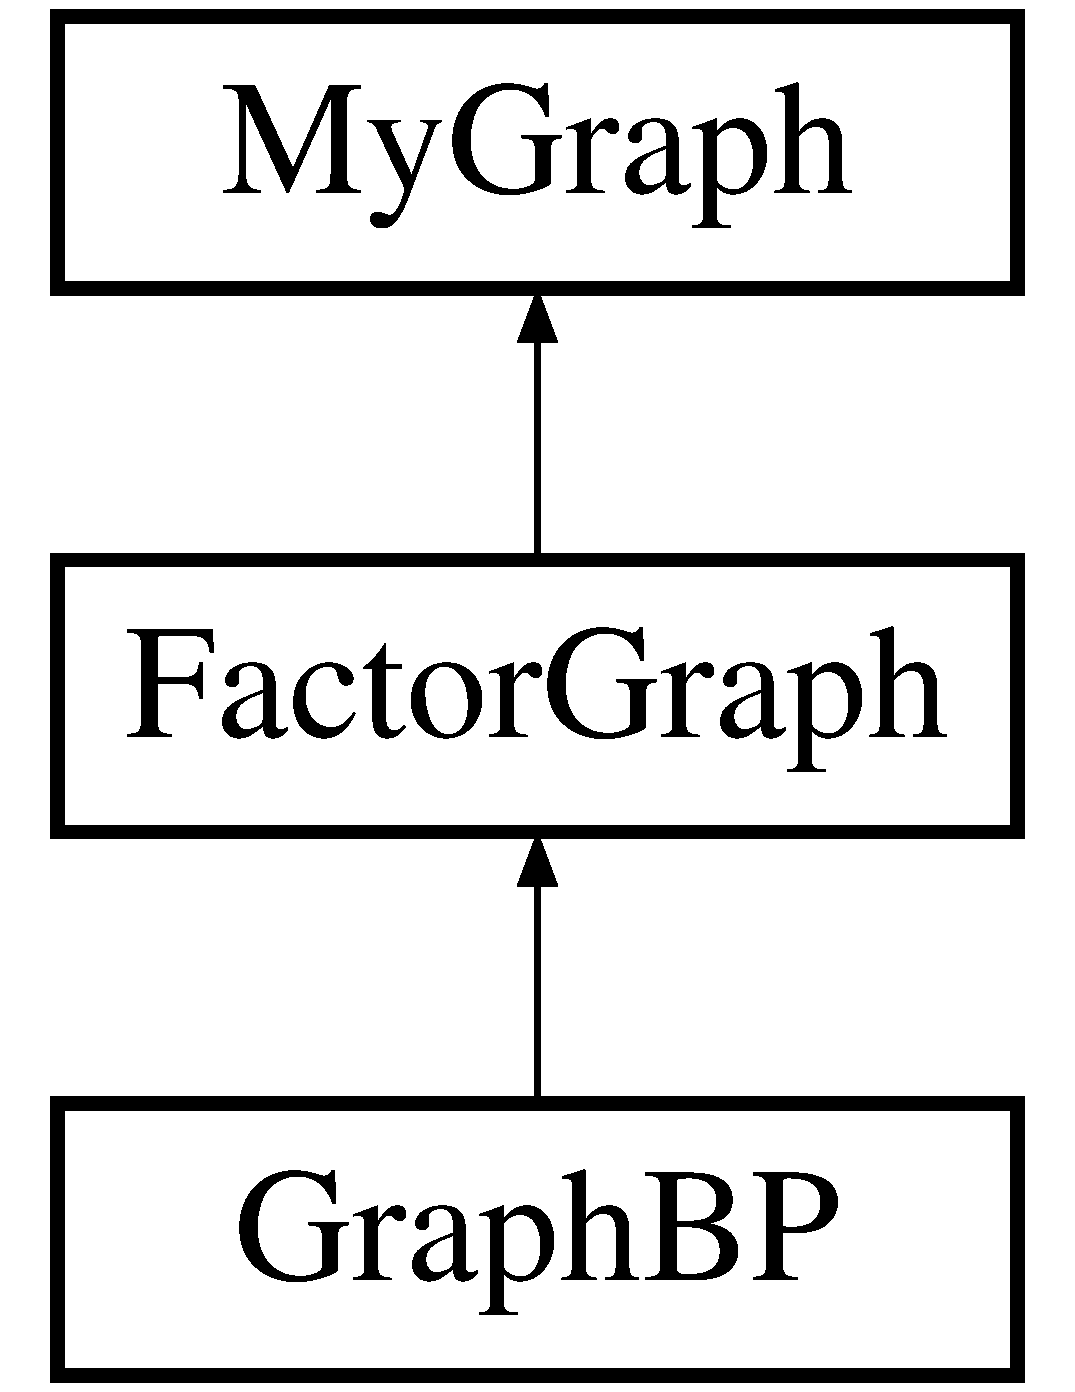
\includegraphics[height=3cm]{classGraphBP}
\end{center}
\end{figure}
\subsection*{Public Member Functions}
\begin{CompactItemize}
\item 
{\bf GraphBP} ({\bf PottsModel} $\ast$\_\-model)
\item 
pair$<$ {\bf EdgePtr}, {\bf EdgePtr} $>$ {\bf addEdge} (const {\bf NodePtr} \&n1, {\bf NodePtr} const \&n2, bool isParent, bool checkExisting=false)
\item 
pair$<$ {\bf EdgePtr}, {\bf EdgePtr} $>$ {\bf findEdge} ({\bf NodePtr} nps, {\bf NodePtr} npt)
\item 
{\bf LD} {\bf updateM} ({\bf NodePtr} np, {\bf NodePtr} nc)
\begin{CompactList}\small\item\em updates the parent to child message \item\end{CompactList}\item 
{\bf LD} {\bf updateN} ({\bf NodePtr} np, {\bf NodePtr} nc)
\begin{CompactList}\small\item\em updates the child to parent message \item\end{CompactList}\end{CompactItemize}
\subsection*{Private Attributes}
\begin{CompactItemize}
\item 
{\bf PottsModel} $\ast$ {\bf model}
\end{CompactItemize}


\subsection{Constructor \& Destructor Documentation}
\index{GraphBP@{GraphBP}!GraphBP@{GraphBP}}
\index{GraphBP@{GraphBP}!GraphBP@{GraphBP}}
\subsubsection{\setlength{\rightskip}{0pt plus 5cm}GraphBP::GraphBP ({\bf PottsModel} $\ast$ {\em \_\-model})\hspace{0.3cm}{\tt  [inline]}}\label{classGraphBP_b859f66495455d66ac79681572e0e0cc}




\subsection{Member Function Documentation}
\index{GraphBP@{GraphBP}!addEdge@{addEdge}}
\index{addEdge@{addEdge}!GraphBP@{GraphBP}}
\subsubsection{\setlength{\rightskip}{0pt plus 5cm}pair$<$ {\bf EdgePtr}, {\bf EdgePtr} $>$ GraphBP::addEdge (const {\bf NodePtr} \& {\em n1}, {\bf NodePtr} const \& {\em n2}, bool {\em isParent}, bool {\em checkExisting} = {\tt false})}\label{classGraphBP_0c0ad66ea90889ffbd10ab073def4c9c}


\index{GraphBP@{GraphBP}!findEdge@{findEdge}}
\index{findEdge@{findEdge}!GraphBP@{GraphBP}}
\subsubsection{\setlength{\rightskip}{0pt plus 5cm}pair$<$ {\bf EdgePtr}, {\bf EdgePtr} $>$ GraphBP::findEdge ({\bf NodePtr} {\em nps}, {\bf NodePtr} {\em npt})}\label{classGraphBP_3bd3c5f1258fd15987ad585941afeac7}




Reimplemented from {\bf MyGraph} \doxyref{}{p.}{classMyGraph_32d78b2a4559ac47fdbbf6da9cb52e60}.\index{GraphBP@{GraphBP}!updateM@{updateM}}
\index{updateM@{updateM}!GraphBP@{GraphBP}}
\subsubsection{\setlength{\rightskip}{0pt plus 5cm}{\bf LD} GraphBP::updateM ({\bf NodePtr} {\em np}, {\bf NodePtr} {\em nc})}\label{classGraphBP_fad15c72784d57fb7aa87454ad5874d6}


updates the parent to child message 



Reimplemented from {\bf FactorGraph} \doxyref{}{p.}{classFactorGraph_78f6edbe28e6a2006ca2eaeea55f6966}.\index{GraphBP@{GraphBP}!updateN@{updateN}}
\index{updateN@{updateN}!GraphBP@{GraphBP}}
\subsubsection{\setlength{\rightskip}{0pt plus 5cm}{\bf LD} GraphBP::updateN ({\bf NodePtr} {\em np}, {\bf NodePtr} {\em nc})}\label{classGraphBP_9748b687eb66ce93a4c875457a3816ce}


updates the child to parent message 



Reimplemented from {\bf FactorGraph} \doxyref{}{p.}{classFactorGraph_50fe3b70c2cf57b3ff7c885def2d0119}.

\subsection{Member Data Documentation}
\index{GraphBP@{GraphBP}!model@{model}}
\index{model@{model}!GraphBP@{GraphBP}}
\subsubsection{\setlength{\rightskip}{0pt plus 5cm}{\bf PottsModel}$\ast$ {\bf GraphBP::model}\hspace{0.3cm}{\tt  [private]}}\label{classGraphBP_a6f3666f26602e0df6704cb64b21cccd}




The documentation for this class was generated from the following files:\begin{CompactItemize}
\item 
inc/{\bf GraphBP.h}\item 
src/{\bf GraphBP.cpp}\end{CompactItemize}

\section{GraphGBP Class Reference}
\label{classGraphGBP}\index{GraphGBP@{GraphGBP}}
{\tt \#include $<$GraphGBP.h$>$}

Inheritance diagram for GraphGBP::\begin{figure}[H]
\begin{center}
\leavevmode
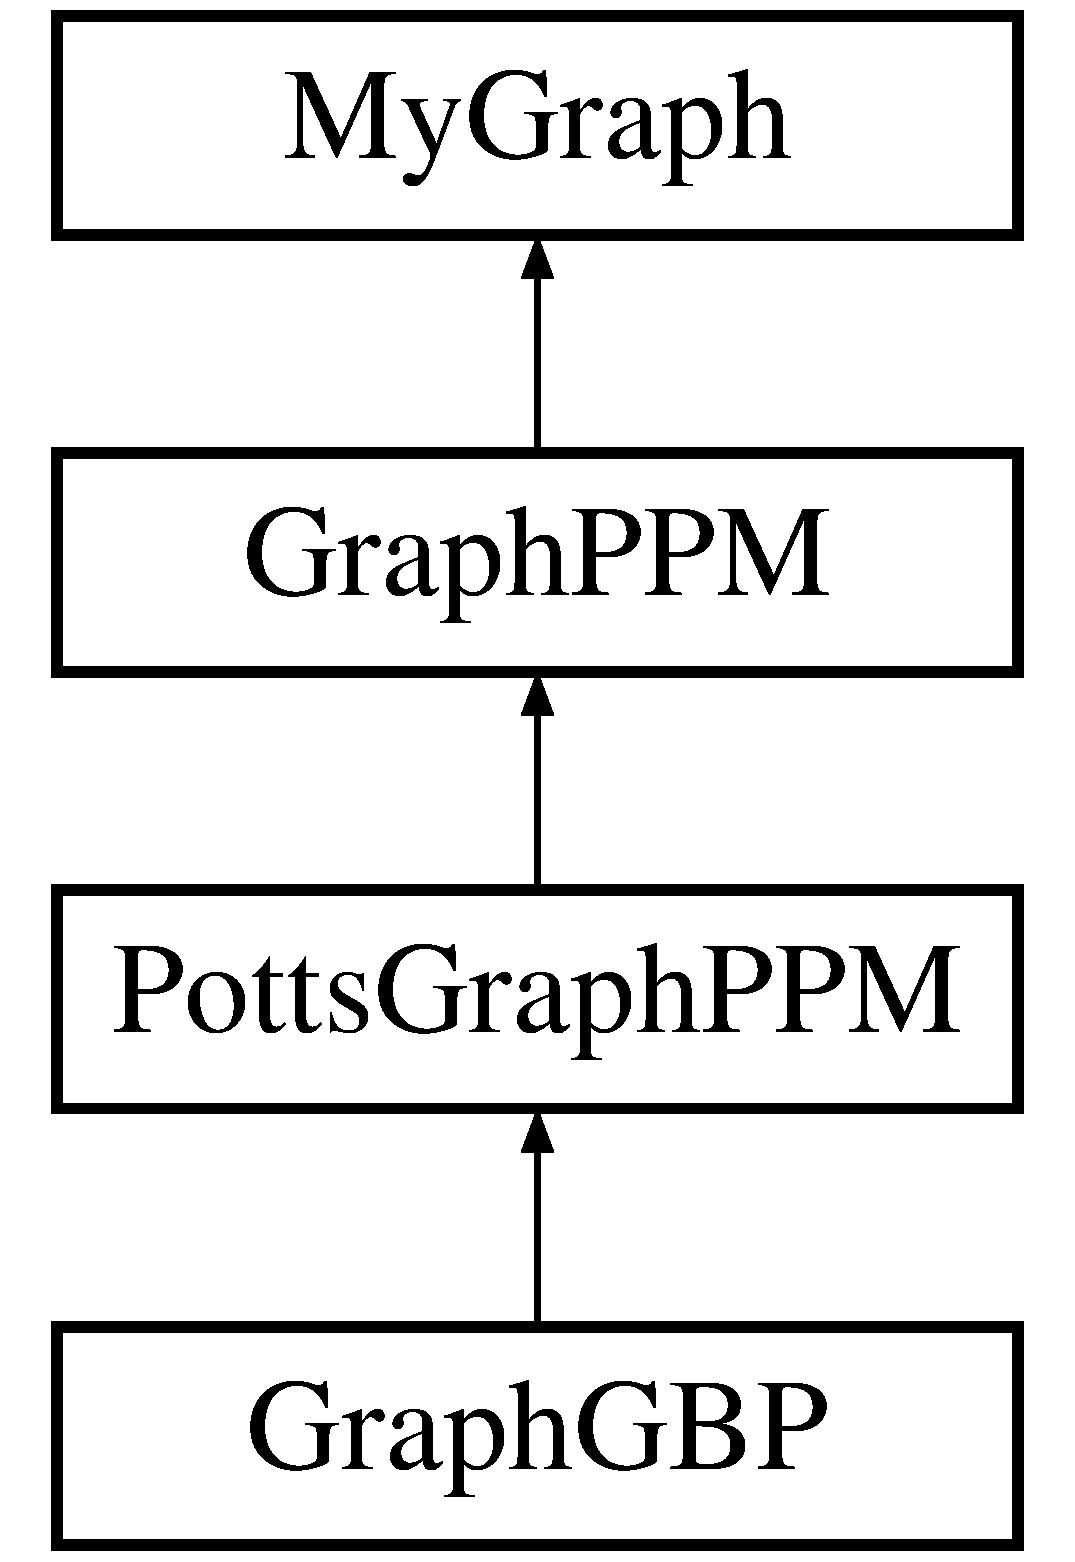
\includegraphics[height=4cm]{classGraphGBP}
\end{center}
\end{figure}
\subsection*{Public Member Functions}
\begin{CompactItemize}
\item 
void {\bf construct\_\-graph} (bool isNodeInitProbRandom, {\bf LD} theta, {\bf LD} {\bf delta\_\-t})
\begin{CompactList}\small\item\em constructs the potts graph and initializes pHat for each node \item\end{CompactList}\item 
void {\bf step\_\-init} ()
\begin{CompactList}\small\item\em initializes all the messages to 1.0 \item\end{CompactList}\item 
void {\bf step\_\-updateJointB} ()
\begin{CompactList}\small\item\em updates the joint belief vectors and stores in \doxyref{RegionPPM::bJointRev}{p.}{classRegionPPM_ae56fc025e98f6e03a8714c0c1b7d59b} \item\end{CompactList}\item 
void {\bf step\_\-updateMpc} ()
\begin{CompactList}\small\item\em updates all child-$>$parent messages \item\end{CompactList}\item 
{\bf GraphGBP} ({\bf PottsModel} $\ast$\_\-M, int \_\-rx, int \_\-ry, int \_\-cx, int \_\-cy)
\begin{CompactList}\small\item\em the constructs that allows construction of \doxyref{PottsModel}{p.}{structPottsModel} based graphs using \doxyref{PottsGraphPPM}{p.}{classPottsGraphPPM} code \item\end{CompactList}\end{CompactItemize}
\subsection*{Protected Member Functions}
\begin{CompactItemize}
\item 
{\bf LD} {\bf lambdaAlphaToParent} ({\bf RegionPPM} $\ast$alpha, {\bf StatePtr} currentState, {\bf StatePtr} nextState)
\begin{CompactList}\small\item\em returns the prod\_\-\{parent\} parent-$>$ region contribution \{DENOMINATOR\} \item\end{CompactList}\item 
{\bf LD} {\bf lambdaChildToAlpha} ({\bf RegionPPM} $\ast$alpha, {\bf StatePtr} currentState, {\bf StatePtr} nextState)
\begin{CompactList}\small\item\em returns the prod\_\-\{child\} child -$>$ region contribution \{NUMERATOR\} \item\end{CompactList}\item 
{\bf LD} {\bf getMalphaUpdate} ({\bf NodePtr} vn)
\begin{CompactList}\small\item\em updates the $m_\alpha$ for given region $\alpha$ \item\end{CompactList}\item 
{\bf LD} {\bf getBeliefUpdate} ({\bf NodePtr} vn, {\bf StatePtr} cs, {\bf StatePtr} ns)
\begin{CompactList}\small\item\em computes the joint belief for given node $\alpha$ \item\end{CompactList}\item 
{\bf LD} {\bf getMpcUpdate} ({\bf NodePtr} vp, {\bf NodePtr} vc, {\bf StatePtr} jointSt)
\begin{CompactList}\small\item\em Computes the parent-$>$child message update. \item\end{CompactList}\end{CompactItemize}


\subsection{Detailed Description}
This class re-implements GBP message passing algorithm as applied to time 



\subsection{Constructor \& Destructor Documentation}
\index{GraphGBP@{GraphGBP}!GraphGBP@{GraphGBP}}
\index{GraphGBP@{GraphGBP}!GraphGBP@{GraphGBP}}
\subsubsection{\setlength{\rightskip}{0pt plus 5cm}GraphGBP::GraphGBP ({\bf PottsModel} $\ast$ {\em \_\-M}, int {\em \_\-rx}, int {\em \_\-ry}, int {\em \_\-cx}, int {\em \_\-cy})\hspace{0.3cm}{\tt  [inline]}}\label{classGraphGBP_d44f8c0bfa981daa70c62f7e5f5ded91}


the constructs that allows construction of \doxyref{PottsModel}{p.}{structPottsModel} based graphs using \doxyref{PottsGraphPPM}{p.}{classPottsGraphPPM} code 



\subsection{Member Function Documentation}
\index{GraphGBP@{GraphGBP}!lambdaAlphaToParent@{lambdaAlphaToParent}}
\index{lambdaAlphaToParent@{lambdaAlphaToParent}!GraphGBP@{GraphGBP}}
\subsubsection{\setlength{\rightskip}{0pt plus 5cm}{\bf LD} GraphGBP::lambdaAlphaToParent ({\bf RegionPPM} $\ast$ {\em vn}, {\bf StatePtr} {\em cs}, {\bf StatePtr} {\em ns})\hspace{0.3cm}{\tt  [protected]}}\label{classGraphGBP_2629b2c90228b37d4e98b58cfbe87609}


returns the prod\_\-\{parent\} parent-$>$ region contribution \{DENOMINATOR\} 

Computes the message contributions from node from its parents \begin{itemize}
\item vn: node ptr $\alpha$ \item cs: node current state $ \vec{x}_\alpha^t$ \item ns: node next state $ \vec{x}_\alpha^{t+\delta t} $ \begin{Desc}
\item[Returns:]$\prod_{\{\gamma:\alpha\subset\gamma\} } m_{\alpha\to\gamma}(\vec{x}^{t,\delta t}_\alpha)$ \end{Desc}
\end{itemize}
\index{GraphGBP@{GraphGBP}!lambdaChildToAlpha@{lambdaChildToAlpha}}
\index{lambdaChildToAlpha@{lambdaChildToAlpha}!GraphGBP@{GraphGBP}}
\subsubsection{\setlength{\rightskip}{0pt plus 5cm}{\bf LD} GraphGBP::lambdaChildToAlpha ({\bf RegionPPM} $\ast$ {\em vn}, {\bf StatePtr} {\em cs}, {\bf StatePtr} {\em nextState})\hspace{0.3cm}{\tt  [protected]}}\label{classGraphGBP_6e801af580679c05387a6bbc6aa376bc}


returns the prod\_\-\{child\} child -$>$ region contribution \{NUMERATOR\} 

Computes all children contribution for given node \begin{itemize}
\item vn: node ptr $\alpha$ \item cs: current node state $ \vec{x}_\alpha^t$ \item ns: next node state $ \vec{x}_\alpha^{t+\delta t} $ \begin{Desc}
\item[Returns:]$\prod_{\{\beta:\beta\subset\alpha\} } m_{\beta\to\alpha}(\vec{x}^{t,\delta t}_\beta)$ \end{Desc}
\end{itemize}
\index{GraphGBP@{GraphGBP}!getMalphaUpdate@{getMalphaUpdate}}
\index{getMalphaUpdate@{getMalphaUpdate}!GraphGBP@{GraphGBP}}
\subsubsection{\setlength{\rightskip}{0pt plus 5cm}{\bf LD} GraphGBP::getMalphaUpdate ({\bf NodePtr} {\em vn})\hspace{0.3cm}{\tt  [protected]}}\label{classGraphGBP_c40e28b82a06839873e5839466adfc5f}


updates the $m_\alpha$ for given region $\alpha$ 

NOTE: uses bJointRev as update scheme $b_\alpha (x^{t+\delta t}, x^{t})$ \begin{itemize}
\item vn the region $\alpha$ to be updated \end{itemize}
\index{GraphGBP@{GraphGBP}!getBeliefUpdate@{getBeliefUpdate}}
\index{getBeliefUpdate@{getBeliefUpdate}!GraphGBP@{GraphGBP}}
\subsubsection{\setlength{\rightskip}{0pt plus 5cm}{\bf LD} GraphGBP::getBeliefUpdate ({\bf NodePtr} {\em vn}, {\bf StatePtr} {\em cs}, {\bf StatePtr} {\em ns})\hspace{0.3cm}{\tt  [protected]}}\label{classGraphGBP_a0b147e78db8df90768e13e35f501b40}


computes the joint belief for given node $\alpha$ 

Computes the belief for region $\alpha$ \begin{itemize}
\item vn region $\alpha$ \item cs current state $\vec{x}_\alpha^{t}$ \item ns next state $\vec{x}_\alpha^{t}$ \begin{Desc}
\item[Returns:]$b_\alpha(x_\alpha^t)\times\frac{\lambda^{t+\delta t | t}(x_\alpha^{t,\delta t})}{e\times m_\alpha^{(i)} }\times \Big\{\frac{\lambda_{child\to\alpha}(x_\alpha^{t,\delta t})}{\lambda_{\alpha\to parent}(x_\alpha^{t,\delta t})}\Big\}^{1/c_\alpha}$ \end{Desc}
\end{itemize}
\index{GraphGBP@{GraphGBP}!getMpcUpdate@{getMpcUpdate}}
\index{getMpcUpdate@{getMpcUpdate}!GraphGBP@{GraphGBP}}
\subsubsection{\setlength{\rightskip}{0pt plus 5cm}{\bf LD} GraphGBP::getMpcUpdate ({\bf NodePtr} {\em vp}, {\bf NodePtr} {\em vc}, {\bf StatePtr} {\em jointSt})\hspace{0.3cm}{\tt  [protected]}}\label{classGraphGBP_11b6c7b6e6b0110642d5c9ef9023867c}


Computes the parent-$>$child message update. 

NOTE: Assumes \doxyref{RegionPPM::bJointRev}{p.}{classRegionPPM_ae56fc025e98f6e03a8714c0c1b7d59b} as $b_\alpha (x^{t+\delta t}, x^t)$ \begin{itemize}
\item vp parent node $\alpha$ \item vc child node $\beta$ \item jointSt child joint state $x_\beta^{t,\delta t}$ \begin{Desc}
\item[Returns:]\[ m_{\beta\to\alpha}^{(i+1)}(x_\beta^{t,\delta t}) = m_{\beta\to\alpha}^{(i)}(x_\beta^{t,\delta t})\times \Big\{\frac{b_\beta^{(i)}(x_\beta^{t, \delta t})}{\sum_{x_\alpha\backslash\beta^{t,\delta t}} b_\alpha^{(i)}(x_\alpha^{t, \delta t})}\Big\}^{\frac{c_\alpha c_\beta}{c_\alpha + c_\beta}}\] \end{Desc}
\end{itemize}
\index{GraphGBP@{GraphGBP}!construct_graph@{construct\_\-graph}}
\index{construct_graph@{construct\_\-graph}!GraphGBP@{GraphGBP}}
\subsubsection{\setlength{\rightskip}{0pt plus 5cm}void GraphGBP::construct\_\-graph (bool {\em isNodeInitProbRandom}, {\bf LD} {\em theta}, {\bf LD} {\em delta\_\-t})}\label{classGraphGBP_ca847b7010619629dcebe4123ab2be94}


constructs the potts graph and initializes pHat for each node 

initializes the potts graph structure (adds nodes/edges) and updates the pHat vector for each node \index{GraphGBP@{GraphGBP}!step_init@{step\_\-init}}
\index{step_init@{step\_\-init}!GraphGBP@{GraphGBP}}
\subsubsection{\setlength{\rightskip}{0pt plus 5cm}void GraphGBP::step\_\-init ()}\label{classGraphGBP_a219d020431022451f3b18ee434892a9}


initializes all the messages to 1.0 

\index{GraphGBP@{GraphGBP}!step_updateJointB@{step\_\-updateJointB}}
\index{step_updateJointB@{step\_\-updateJointB}!GraphGBP@{GraphGBP}}
\subsubsection{\setlength{\rightskip}{0pt plus 5cm}void GraphGBP::step\_\-updateJointB ()}\label{classGraphGBP_098b976e1c573a65b1e45a8ec19a0306}


updates the joint belief vectors and stores in \doxyref{RegionPPM::bJointRev}{p.}{classRegionPPM_ae56fc025e98f6e03a8714c0c1b7d59b} 

\index{GraphGBP@{GraphGBP}!step_updateMpc@{step\_\-updateMpc}}
\index{step_updateMpc@{step\_\-updateMpc}!GraphGBP@{GraphGBP}}
\subsubsection{\setlength{\rightskip}{0pt plus 5cm}void GraphGBP::step\_\-updateMpc ()}\label{classGraphGBP_7d56c8d1681e1c718d37101a04ff8a68}


updates all child-$>$parent messages 

NOTE: Assumes \doxyref{RegionPPM::bJointRev}{p.}{classRegionPPM_ae56fc025e98f6e03a8714c0c1b7d59b} correctly initialized 

The documentation for this class was generated from the following files:\begin{CompactItemize}
\item 
inc/{\bf GraphGBP.h}\item 
src/{\bf GraphGBP.cpp}\end{CompactItemize}

\section{GraphMVI Class Reference}
\label{classGraphMVI}\index{GraphMVI@{GraphMVI}}
{\tt \#include $<$MVI.h$>$}

Inheritance diagram for GraphMVI::\begin{figure}[H]
\begin{center}
\leavevmode
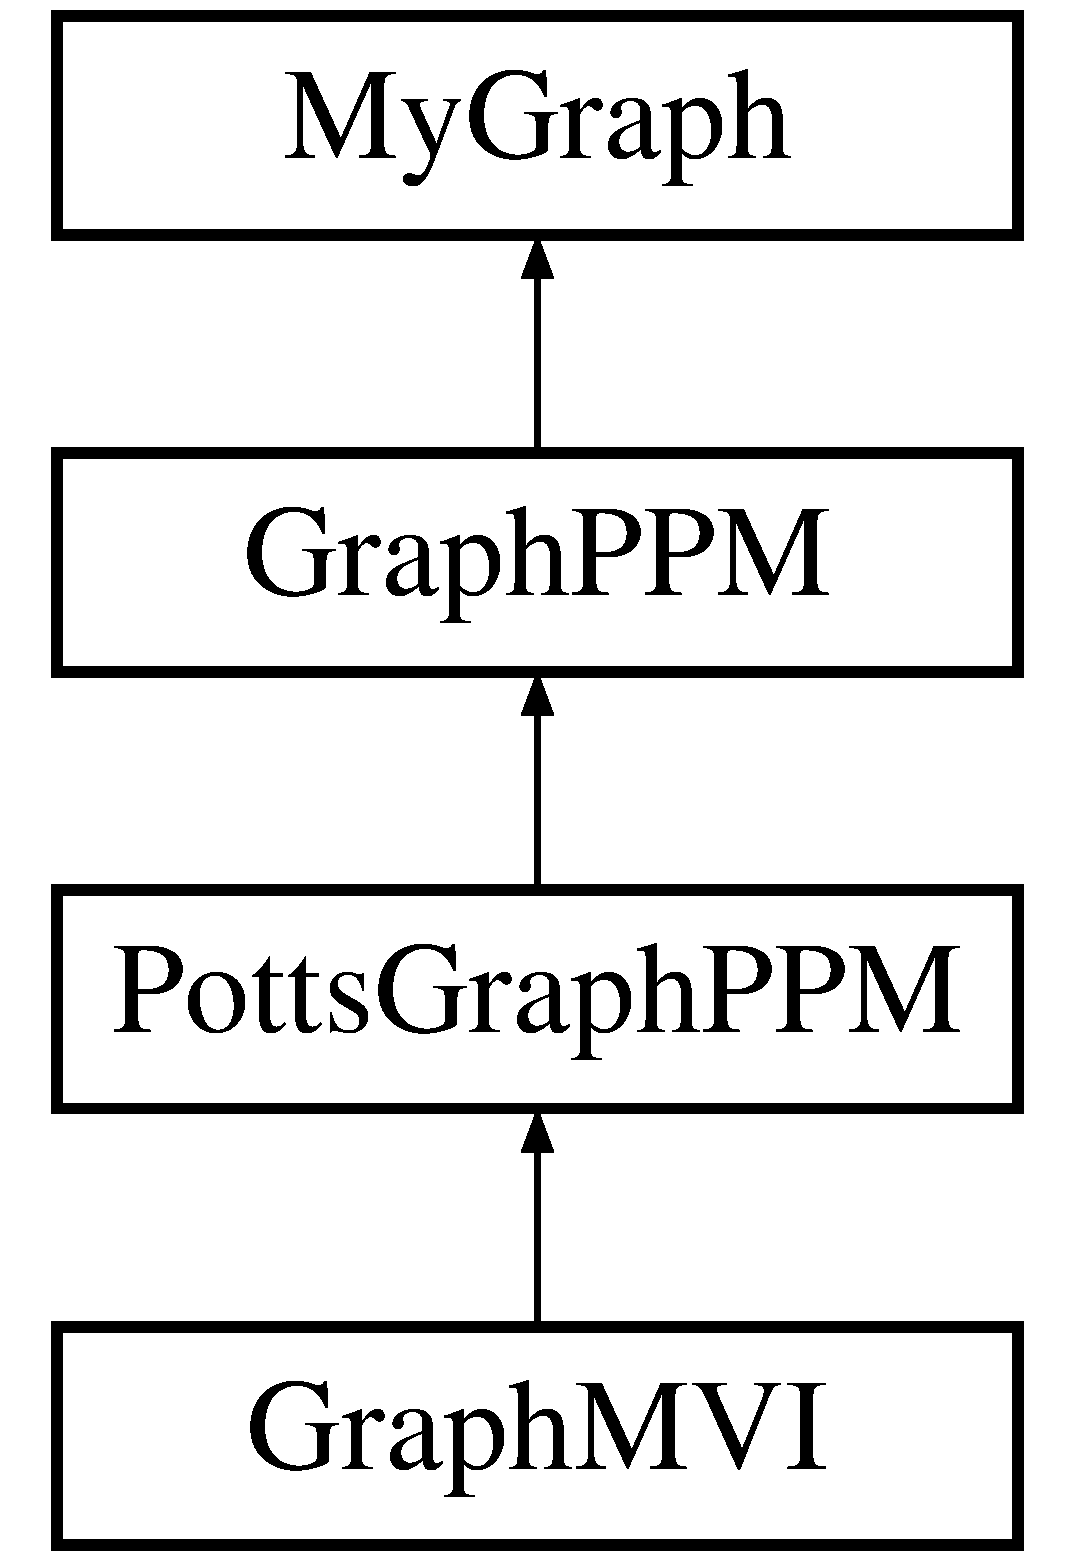
\includegraphics[height=4cm]{classGraphMVI}
\end{center}
\end{figure}
\subsection*{Public Member Functions}
\begin{CompactItemize}
\item 
{\bf LD} {\bf get\_\-p\_\-t} (int i, int j, {\bf INT} xi, {\bf INT} xo)
\item 
{\bf LD} {\bf getStatePr} ({\bf VideoNode} $\ast$vn, {\bf StatePtr} sp)
\item 
{\bf GraphMVI} ({\bf LD} S, {\bf LD} T, {\bf ModelMVI} $\ast$\_\-M, int \_\-rx=2, int \_\-ry=2, int \_\-cx=1, int \_\-cy=1)
\item 
void {\bf update\_\-evidence} (vector$<$ vector$<$ {\bf INT} $>$ $>$ \_\-evidence)
\item 
vector$<$ vector$<$ {\bf INT} $>$ $>$ {\bf map\_\-estimate} ()
\item 
vector$<$ vector$<$ {\bf INT} $>$ $>$ {\bf mmse\_\-estimate} ()
\item 
{\bf LD} {\bf get\_\-p\_\-hat} ({\bf VideoNode} $\ast$vn, {\bf StatePtr} si, {\bf StatePtr} so, {\bf LD} theta, {\bf LD} dt)
\item 
void {\bf initCondP} ({\bf VideoNode} $\ast$vn, {\bf LD} theta, {\bf LD} dt)
\item 
{\bf LD} {\bf updateTime} ({\bf LD} dt)
\item 
void {\bf initAllNodesOrigP} (bool rndm=false)
\end{CompactItemize}
\subsection*{Private Attributes}
\begin{CompactItemize}
\item 
{\bf LD} {\bf theta\_\-r}
\item 
{\bf LD} {\bf theta\_\-t}
\item 
{\bf LD} {\bf epsilon\_\-r}
\item 
{\bf LD} {\bf epsilon\_\-t}
\item 
{\bf LD} {\bf epsilon\_\-zero}
\item 
vector$<$ vector$<$ {\bf INT} $>$ $>$ {\bf evidence}
\item 
int {\bf C}
\item 
int {\bf N1}
\item 
int {\bf N2}
\item 
{\bf StatePtr} {\bf ST} [2]
\item 
{\bf StatePtr} {\bf SC}
\end{CompactItemize}


\subsection{Constructor \& Destructor Documentation}
\index{GraphMVI@{GraphMVI}!GraphMVI@{GraphMVI}}
\index{GraphMVI@{GraphMVI}!GraphMVI@{GraphMVI}}
\subsubsection{\setlength{\rightskip}{0pt plus 5cm}GraphMVI::GraphMVI ({\bf LD} {\em S}, {\bf LD} {\em T}, {\bf ModelMVI} $\ast$ {\em \_\-M}, int {\em \_\-rx} = {\tt 2}, int {\em \_\-ry} = {\tt 2}, int {\em \_\-cx} = {\tt 1}, int {\em \_\-cy} = {\tt 1})\hspace{0.3cm}{\tt  [inline]}}\label{classGraphMVI_d5b8b05a142fecc8ae10b5b2d39f563a}




\subsection{Member Function Documentation}
\index{GraphMVI@{GraphMVI}!get_p_t@{get\_\-p\_\-t}}
\index{get_p_t@{get\_\-p\_\-t}!GraphMVI@{GraphMVI}}
\subsubsection{\setlength{\rightskip}{0pt plus 5cm}{\bf LD} GraphMVI::get\_\-p\_\-t (int {\em i}, int {\em j}, {\bf INT} {\em xi}, {\bf INT} {\em xo})}\label{classGraphMVI_a767afbe4ff9fe4286790d7f78d63847}


\index{GraphMVI@{GraphMVI}!getStatePr@{getStatePr}}
\index{getStatePr@{getStatePr}!GraphMVI@{GraphMVI}}
\subsubsection{\setlength{\rightskip}{0pt plus 5cm}{\bf LD} GraphMVI::getStatePr ({\bf VideoNode} $\ast$ {\em vn}, {\bf StatePtr} {\em sp})\hspace{0.3cm}{\tt  [inline]}}\label{classGraphMVI_8751683935447989fb988382955dbc02}




Reimplemented from {\bf PottsGraphPPM} \doxyref{}{p.}{classPottsGraphPPM_03ceec5a5ddb5b33d1b1acb2926265b9}.\index{GraphMVI@{GraphMVI}!update_evidence@{update\_\-evidence}}
\index{update_evidence@{update\_\-evidence}!GraphMVI@{GraphMVI}}
\subsubsection{\setlength{\rightskip}{0pt plus 5cm}void GraphMVI::update\_\-evidence (vector$<$ vector$<$ {\bf INT} $>$ $>$ {\em \_\-evidence})\hspace{0.3cm}{\tt  [inline]}}\label{classGraphMVI_316b9b81078bd65bb17c9b779bc3bba3}


\index{GraphMVI@{GraphMVI}!map_estimate@{map\_\-estimate}}
\index{map_estimate@{map\_\-estimate}!GraphMVI@{GraphMVI}}
\subsubsection{\setlength{\rightskip}{0pt plus 5cm}vector$<$ vector$<$ {\bf INT} $>$ $>$ GraphMVI::map\_\-estimate ()}\label{classGraphMVI_d3340d9ddcac2170592fa7d5816f48f8}


\index{GraphMVI@{GraphMVI}!mmse_estimate@{mmse\_\-estimate}}
\index{mmse_estimate@{mmse\_\-estimate}!GraphMVI@{GraphMVI}}
\subsubsection{\setlength{\rightskip}{0pt plus 5cm}vector$<$ vector$<$ {\bf INT} $>$ $>$ GraphMVI::mmse\_\-estimate ()}\label{classGraphMVI_dde7afa5bda9d24e70b45fba142a2c68}


\index{GraphMVI@{GraphMVI}!get_p_hat@{get\_\-p\_\-hat}}
\index{get_p_hat@{get\_\-p\_\-hat}!GraphMVI@{GraphMVI}}
\subsubsection{\setlength{\rightskip}{0pt plus 5cm}{\bf LD} GraphMVI::get\_\-p\_\-hat ({\bf VideoNode} $\ast$ {\em vn}, {\bf StatePtr} {\em si}, {\bf StatePtr} {\em so}, {\bf LD} {\em theta}, {\bf LD} {\em dt})}\label{classGraphMVI_f2a1f00572448ffe7568d0c927bfcc51}




Reimplemented from {\bf PottsGraphPPM} \doxyref{}{p.}{classPottsGraphPPM_b735fb1d57301afad4cdc14ffd5a6252}.\index{GraphMVI@{GraphMVI}!initCondP@{initCondP}}
\index{initCondP@{initCondP}!GraphMVI@{GraphMVI}}
\subsubsection{\setlength{\rightskip}{0pt plus 5cm}void GraphMVI::initCondP ({\bf VideoNode} $\ast$ {\em vn}, {\bf LD} {\em theta}, {\bf LD} {\em dt})}\label{classGraphMVI_5137366e48b2928a20236e8851ae5e4b}




Reimplemented from {\bf PottsGraphPPM} \doxyref{}{p.}{classPottsGraphPPM_276673597baefb6b317b96efe23815fa}.\index{GraphMVI@{GraphMVI}!updateTime@{updateTime}}
\index{updateTime@{updateTime}!GraphMVI@{GraphMVI}}
\subsubsection{\setlength{\rightskip}{0pt plus 5cm}{\bf LD} GraphMVI::updateTime ({\bf LD} {\em dt})}\label{classGraphMVI_25b13c96f42a85b5ed3d7e6068e1659c}




Reimplemented from {\bf PottsGraphPPM} \doxyref{}{p.}{classPottsGraphPPM_9cac6ffa0063ec4e5a3102f93bd2da92}.\index{GraphMVI@{GraphMVI}!initAllNodesOrigP@{initAllNodesOrigP}}
\index{initAllNodesOrigP@{initAllNodesOrigP}!GraphMVI@{GraphMVI}}
\subsubsection{\setlength{\rightskip}{0pt plus 5cm}void GraphMVI::initAllNodesOrigP (bool {\em rndm} = {\tt false})}\label{classGraphMVI_1033e03be9c66b7ff356c7bb0e8fe083}




Reimplemented from {\bf PottsGraphPPM} \doxyref{}{p.}{classPottsGraphPPM_db429e7e4eac1a4d69f641403735cb20}.

\subsection{Member Data Documentation}
\index{GraphMVI@{GraphMVI}!theta_r@{theta\_\-r}}
\index{theta_r@{theta\_\-r}!GraphMVI@{GraphMVI}}
\subsubsection{\setlength{\rightskip}{0pt plus 5cm}{\bf LD} {\bf GraphMVI::theta\_\-r}\hspace{0.3cm}{\tt  [private]}}\label{classGraphMVI_72546502639b8985a7eed3326efc51ab}


\index{GraphMVI@{GraphMVI}!theta_t@{theta\_\-t}}
\index{theta_t@{theta\_\-t}!GraphMVI@{GraphMVI}}
\subsubsection{\setlength{\rightskip}{0pt plus 5cm}{\bf LD} {\bf GraphMVI::theta\_\-t}\hspace{0.3cm}{\tt  [private]}}\label{classGraphMVI_503ebff4b068dab18993f4fa0c6c8c74}


\index{GraphMVI@{GraphMVI}!epsilon_r@{epsilon\_\-r}}
\index{epsilon_r@{epsilon\_\-r}!GraphMVI@{GraphMVI}}
\subsubsection{\setlength{\rightskip}{0pt plus 5cm}{\bf LD} {\bf GraphMVI::epsilon\_\-r}\hspace{0.3cm}{\tt  [private]}}\label{classGraphMVI_540ee4df899efdef389e444720bfbe42}


\index{GraphMVI@{GraphMVI}!epsilon_t@{epsilon\_\-t}}
\index{epsilon_t@{epsilon\_\-t}!GraphMVI@{GraphMVI}}
\subsubsection{\setlength{\rightskip}{0pt plus 5cm}{\bf LD} {\bf GraphMVI::epsilon\_\-t}\hspace{0.3cm}{\tt  [private]}}\label{classGraphMVI_48a29ed771ce345f053b901869d30b50}


\index{GraphMVI@{GraphMVI}!epsilon_zero@{epsilon\_\-zero}}
\index{epsilon_zero@{epsilon\_\-zero}!GraphMVI@{GraphMVI}}
\subsubsection{\setlength{\rightskip}{0pt plus 5cm}{\bf LD} {\bf GraphMVI::epsilon\_\-zero}\hspace{0.3cm}{\tt  [private]}}\label{classGraphMVI_fe25b2ab52847613d5337ebc8732f753}


\index{GraphMVI@{GraphMVI}!evidence@{evidence}}
\index{evidence@{evidence}!GraphMVI@{GraphMVI}}
\subsubsection{\setlength{\rightskip}{0pt plus 5cm}vector$<$vector$<${\bf INT}$>$ $>$ {\bf GraphMVI::evidence}\hspace{0.3cm}{\tt  [private]}}\label{classGraphMVI_20fd7ea85ce95b60c14f6211faec4b89}


\index{GraphMVI@{GraphMVI}!C@{C}}
\index{C@{C}!GraphMVI@{GraphMVI}}
\subsubsection{\setlength{\rightskip}{0pt plus 5cm}int {\bf GraphMVI::C}\hspace{0.3cm}{\tt  [private]}}\label{classGraphMVI_3e1fab43a7c8648774b4ea32734e32ec}


\index{GraphMVI@{GraphMVI}!N1@{N1}}
\index{N1@{N1}!GraphMVI@{GraphMVI}}
\subsubsection{\setlength{\rightskip}{0pt plus 5cm}int {\bf GraphMVI::N1}\hspace{0.3cm}{\tt  [private]}}\label{classGraphMVI_5a96b3447f47f5f9fd3468edc63de8e4}


\index{GraphMVI@{GraphMVI}!N2@{N2}}
\index{N2@{N2}!GraphMVI@{GraphMVI}}
\subsubsection{\setlength{\rightskip}{0pt plus 5cm}int {\bf GraphMVI::N2}\hspace{0.3cm}{\tt  [private]}}\label{classGraphMVI_55cb4e937c09f5da834a8088dfd93720}


\index{GraphMVI@{GraphMVI}!ST@{ST}}
\index{ST@{ST}!GraphMVI@{GraphMVI}}
\subsubsection{\setlength{\rightskip}{0pt plus 5cm}{\bf StatePtr} {\bf GraphMVI::ST}[2]\hspace{0.3cm}{\tt  [private]}}\label{classGraphMVI_b0260ff565bfdbd01f8a689a4554605a}


\index{GraphMVI@{GraphMVI}!SC@{SC}}
\index{SC@{SC}!GraphMVI@{GraphMVI}}
\subsubsection{\setlength{\rightskip}{0pt plus 5cm}{\bf StatePtr} {\bf GraphMVI::SC}\hspace{0.3cm}{\tt  [private]}}\label{classGraphMVI_42de04cbb4ccaf383c3deff1a005d1e9}




The documentation for this class was generated from the following files:\begin{CompactItemize}
\item 
inc/{\bf MVI.h}\item 
src/{\bf MVI.cpp}\end{CompactItemize}

\section{GraphPPM Class Reference}
\label{classGraphPPM}\index{GraphPPM@{GraphPPM}}
{\tt \#include $<$GraphPPM.h$>$}

Inheritance diagram for GraphPPM::\begin{figure}[H]
\begin{center}
\leavevmode
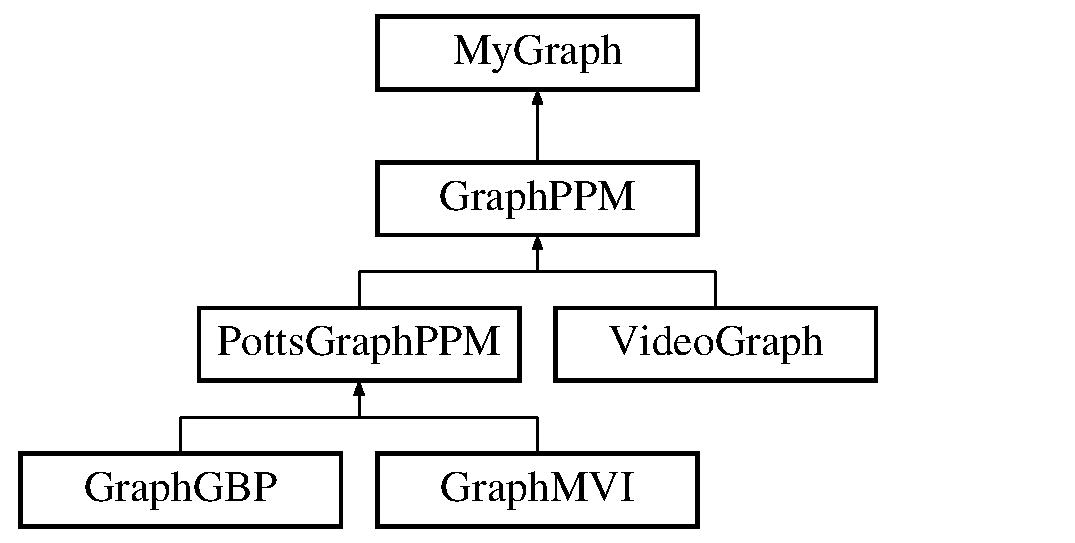
\includegraphics[height=4cm]{classGraphPPM}
\end{center}
\end{figure}
\subsection*{Public Member Functions}
\begin{CompactItemize}
\item 
{\bf StatePtr} {\bf getJointState} ({\bf StatePtr} currSt, {\bf StatePtr} nextSt)
\begin{CompactList}\small\item\em initialize all messages \item\end{CompactList}\item 
void {\bf PPM\_\-inner\_\-loop} ()
\item 
void {\bf PPM\_\-step3} ()
\item 
void {\bf PPM\_\-step4a} ()
\item 
void {\bf PPM\_\-step4b} ()
\item 
void {\bf PPM\_\-step5a} ()
\item 
void {\bf PPM\_\-step5b} ()
\item 
void {\bf PPM\_\-step5c} ()
\item 
virtual {\bf StatePtr} {\bf getChildStatePtr} ({\bf NodePtr} vp, {\bf NodePtr} vc, {\bf StatePtr} parState)=0
\item 
void {\bf updateNodesInfo} ()
\item 
string {\bf get\_\-status} ()
\item 
void {\bf PPM\_\-LN} ({\bf LD} thetaLN=1.0)
\begin{CompactList}\small\item\em does the log normalization on the messages \item\end{CompactList}\end{CompactItemize}
\subsection*{Public Attributes}
\begin{CompactItemize}
\item 
{\bf LD} {\bf SR}
\item 
{\bf LD} {\bf minMsg}
\item 
{\bf LD} {\bf maxMsg}
\item 
{\bf LD} {\bf avgDiffFromPars}
\item 
{\bf LD} {\bf avgChngInBlfs}
\item 
{\bf LD} {\bf maxChngInBlfs}
\item 
{\bf LD} {\bf maxDevFromPars}
\item 
{\bf LD} {\bf avgMaxCaseDevFromPars}
\item 
{\bf LD} {\bf avgMaxCaseChngInBlfs}
\end{CompactItemize}
\subsection*{Private Member Functions}
\begin{CompactItemize}
\item 
{\bf LD} {\bf getMargPr\_\-5c} ({\bf RegionPPM} $\ast$vp, {\bf RegionPPM} $\ast$vc, {\bf StatePtr} cStOld, {\bf StatePtr} cStNew)
\end{CompactItemize}


\subsection{Detailed Description}
Graph that implements PPM with partial state space 



\subsection{Member Function Documentation}
\index{GraphPPM@{GraphPPM}!getMargPr_5c@{getMargPr\_\-5c}}
\index{getMargPr_5c@{getMargPr\_\-5c}!GraphPPM@{GraphPPM}}
\subsubsection{\setlength{\rightskip}{0pt plus 5cm}{\bf LD} GraphPPM::getMargPr\_\-5c ({\bf RegionPPM} $\ast$ {\em vp}, {\bf RegionPPM} $\ast$ {\em vc}, {\bf StatePtr} {\em cStOld}, {\bf StatePtr} {\em cStNew})\hspace{0.3cm}{\tt  [private]}}\label{classGraphPPM_b8a6e0a32d1c766f330a4b586dffda03}


\index{GraphPPM@{GraphPPM}!getJointState@{getJointState}}
\index{getJointState@{getJointState}!GraphPPM@{GraphPPM}}
\subsubsection{\setlength{\rightskip}{0pt plus 5cm}{\bf StatePtr} GraphPPM::getJointState ({\bf StatePtr} {\em currSt}, {\bf StatePtr} {\em nextSt})\hspace{0.3cm}{\tt  [inline]}}\label{classGraphPPM_988f1c3b64f4edef454303e21c73897f}


initialize all messages 

\index{GraphPPM@{GraphPPM}!PPM_inner_loop@{PPM\_\-inner\_\-loop}}
\index{PPM_inner_loop@{PPM\_\-inner\_\-loop}!GraphPPM@{GraphPPM}}
\subsubsection{\setlength{\rightskip}{0pt plus 5cm}void GraphPPM::PPM\_\-inner\_\-loop ()}\label{classGraphPPM_af11be7c070e2bf7004b26c4f83a46c4}


\index{GraphPPM@{GraphPPM}!PPM_step3@{PPM\_\-step3}}
\index{PPM_step3@{PPM\_\-step3}!GraphPPM@{GraphPPM}}
\subsubsection{\setlength{\rightskip}{0pt plus 5cm}void GraphPPM::PPM\_\-step3 ()}\label{classGraphPPM_948e40d894af5e3dbe6c74261ad7dce0}


Initializes child-$>$parent messages (child-$>$BidirEdgeList.second) to 1.0 for all nodes. Note: PPM/GBP child-$>$parent algorithm does not use forward messages from parent-$>$child. \index{GraphPPM@{GraphPPM}!PPM_step4a@{PPM\_\-step4a}}
\index{PPM_step4a@{PPM\_\-step4a}!GraphPPM@{GraphPPM}}
\subsubsection{\setlength{\rightskip}{0pt plus 5cm}void GraphPPM::PPM\_\-step4a ()}\label{classGraphPPM_a18d082afd8695ff634e96c9df275252}


\index{GraphPPM@{GraphPPM}!PPM_step4b@{PPM\_\-step4b}}
\index{PPM_step4b@{PPM\_\-step4b}!GraphPPM@{GraphPPM}}
\subsubsection{\setlength{\rightskip}{0pt plus 5cm}void GraphPPM::PPM\_\-step4b ()}\label{classGraphPPM_662bcc5d8e432d5275c1397c08393704}


\index{GraphPPM@{GraphPPM}!PPM_step5a@{PPM\_\-step5a}}
\index{PPM_step5a@{PPM\_\-step5a}!GraphPPM@{GraphPPM}}
\subsubsection{\setlength{\rightskip}{0pt plus 5cm}void GraphPPM::PPM\_\-step5a ()}\label{classGraphPPM_beb37a3d5d63d04a0df4843a158207bc}


\index{GraphPPM@{GraphPPM}!PPM_step5b@{PPM\_\-step5b}}
\index{PPM_step5b@{PPM\_\-step5b}!GraphPPM@{GraphPPM}}
\subsubsection{\setlength{\rightskip}{0pt plus 5cm}void GraphPPM::PPM\_\-step5b ()}\label{classGraphPPM_7f8b5da78e79027f06093f304f9adac7}


\index{GraphPPM@{GraphPPM}!PPM_step5c@{PPM\_\-step5c}}
\index{PPM_step5c@{PPM\_\-step5c}!GraphPPM@{GraphPPM}}
\subsubsection{\setlength{\rightskip}{0pt plus 5cm}void GraphPPM::PPM\_\-step5c ()}\label{classGraphPPM_0a3e53cd03010beaee032d73ce4de071}


\index{GraphPPM@{GraphPPM}!getChildStatePtr@{getChildStatePtr}}
\index{getChildStatePtr@{getChildStatePtr}!GraphPPM@{GraphPPM}}
\subsubsection{\setlength{\rightskip}{0pt plus 5cm}virtual {\bf StatePtr} GraphPPM::getChildStatePtr ({\bf NodePtr} {\em vp}, {\bf NodePtr} {\em vc}, {\bf StatePtr} {\em parState})\hspace{0.3cm}{\tt  [pure virtual]}}\label{classGraphPPM_b245aae058d0b252df985651c8fcc2eb}




Implemented in {\bf PottsGraphPPM} \doxyref{}{p.}{classPottsGraphPPM_7422e923b897b8799ab7de73e3f10088}, and {\bf VideoGraph} \doxyref{}{p.}{classVideoGraph_9e6275280e01ab9b37b52e7cf92ddd2d}.\index{GraphPPM@{GraphPPM}!updateNodesInfo@{updateNodesInfo}}
\index{updateNodesInfo@{updateNodesInfo}!GraphPPM@{GraphPPM}}
\subsubsection{\setlength{\rightskip}{0pt plus 5cm}void GraphPPM::updateNodesInfo ()}\label{classGraphPPM_63bd812c334b282a1dbba62519672ebe}


\index{GraphPPM@{GraphPPM}!get_status@{get\_\-status}}
\index{get_status@{get\_\-status}!GraphPPM@{GraphPPM}}
\subsubsection{\setlength{\rightskip}{0pt plus 5cm}string GraphPPM::get\_\-status ()}\label{classGraphPPM_0dff6791d6fc383414dfe3dd52162c98}


\index{GraphPPM@{GraphPPM}!PPM_LN@{PPM\_\-LN}}
\index{PPM_LN@{PPM\_\-LN}!GraphPPM@{GraphPPM}}
\subsubsection{\setlength{\rightskip}{0pt plus 5cm}void GraphPPM::PPM\_\-LN ({\bf LD} {\em thetaLN} = {\tt 1.0})}\label{classGraphPPM_0460a9fa53963d976f7c724ad95570e2}


does the log normalization on the messages 



\subsection{Member Data Documentation}
\index{GraphPPM@{GraphPPM}!SR@{SR}}
\index{SR@{SR}!GraphPPM@{GraphPPM}}
\subsubsection{\setlength{\rightskip}{0pt plus 5cm}{\bf LD} {\bf GraphPPM::SR}}\label{classGraphPPM_40944c27ce4ffc3125be88dbc541285c}


\index{GraphPPM@{GraphPPM}!minMsg@{minMsg}}
\index{minMsg@{minMsg}!GraphPPM@{GraphPPM}}
\subsubsection{\setlength{\rightskip}{0pt plus 5cm}{\bf LD} {\bf GraphPPM::minMsg}}\label{classGraphPPM_06945ee22fa9aa7d63a471749b5f4a79}


\index{GraphPPM@{GraphPPM}!maxMsg@{maxMsg}}
\index{maxMsg@{maxMsg}!GraphPPM@{GraphPPM}}
\subsubsection{\setlength{\rightskip}{0pt plus 5cm}{\bf LD} {\bf GraphPPM::maxMsg}}\label{classGraphPPM_a0a25a7a902cce9602754fe8a4b1c79f}


\index{GraphPPM@{GraphPPM}!avgDiffFromPars@{avgDiffFromPars}}
\index{avgDiffFromPars@{avgDiffFromPars}!GraphPPM@{GraphPPM}}
\subsubsection{\setlength{\rightskip}{0pt plus 5cm}{\bf LD} {\bf GraphPPM::avgDiffFromPars}}\label{classGraphPPM_c9f9872b503ee29b1f4558525d47d4d3}


\index{GraphPPM@{GraphPPM}!avgChngInBlfs@{avgChngInBlfs}}
\index{avgChngInBlfs@{avgChngInBlfs}!GraphPPM@{GraphPPM}}
\subsubsection{\setlength{\rightskip}{0pt plus 5cm}{\bf LD} {\bf GraphPPM::avgChngInBlfs}}\label{classGraphPPM_f6cdf67c40cc18f2bdd90b6ec27ea325}


\index{GraphPPM@{GraphPPM}!maxChngInBlfs@{maxChngInBlfs}}
\index{maxChngInBlfs@{maxChngInBlfs}!GraphPPM@{GraphPPM}}
\subsubsection{\setlength{\rightskip}{0pt plus 5cm}{\bf LD} {\bf GraphPPM::maxChngInBlfs}}\label{classGraphPPM_43819d4c1be286f4076b90dd107088f5}


\index{GraphPPM@{GraphPPM}!maxDevFromPars@{maxDevFromPars}}
\index{maxDevFromPars@{maxDevFromPars}!GraphPPM@{GraphPPM}}
\subsubsection{\setlength{\rightskip}{0pt plus 5cm}{\bf LD} {\bf GraphPPM::maxDevFromPars}}\label{classGraphPPM_49b0a168ed985205a4eb9f3977a688b1}


\index{GraphPPM@{GraphPPM}!avgMaxCaseDevFromPars@{avgMaxCaseDevFromPars}}
\index{avgMaxCaseDevFromPars@{avgMaxCaseDevFromPars}!GraphPPM@{GraphPPM}}
\subsubsection{\setlength{\rightskip}{0pt plus 5cm}{\bf LD} {\bf GraphPPM::avgMaxCaseDevFromPars}}\label{classGraphPPM_e0eaf165a890a107506715b5511c4d6e}


\index{GraphPPM@{GraphPPM}!avgMaxCaseChngInBlfs@{avgMaxCaseChngInBlfs}}
\index{avgMaxCaseChngInBlfs@{avgMaxCaseChngInBlfs}!GraphPPM@{GraphPPM}}
\subsubsection{\setlength{\rightskip}{0pt plus 5cm}{\bf LD} {\bf GraphPPM::avgMaxCaseChngInBlfs}}\label{classGraphPPM_4bdc1edbb20d079ac83cff42540989bb}




The documentation for this class was generated from the following files:\begin{CompactItemize}
\item 
inc/{\bf GraphPPM.h}\item 
src/{\bf GraphPPM.cpp}\end{CompactItemize}

\section{GraphProperty Struct Reference}
\label{structGraphProperty}\index{GraphProperty@{GraphProperty}}
{\tt \#include $<$bpgraph.h$>$}

\subsection*{Public Attributes}
\begin{CompactItemize}
\item 
string {\bf name}
\item 
int {\bf numVal}
\end{CompactItemize}


\subsection{Member Data Documentation}
\index{GraphProperty@{GraphProperty}!name@{name}}
\index{name@{name}!GraphProperty@{GraphProperty}}
\subsubsection{\setlength{\rightskip}{0pt plus 5cm}string {\bf GraphProperty::name}}\label{structGraphProperty_be7e304528e5cfc9b0a49f75c12d1bed}


\index{GraphProperty@{GraphProperty}!numVal@{numVal}}
\index{numVal@{numVal}!GraphProperty@{GraphProperty}}
\subsubsection{\setlength{\rightskip}{0pt plus 5cm}int {\bf GraphProperty::numVal}}\label{structGraphProperty_429b5800a147bc2f897ed9e03f87a5a8}




The documentation for this struct was generated from the following file:\begin{CompactItemize}
\item 
inc/{\bf bpgraph.h}\end{CompactItemize}

\section{Image$<$ T $>$ Class Template Reference}
\label{classImage}\index{Image@{Image}}
{\tt \#include $<$Image.h$>$}

\subsection*{Public Member Functions}
\begin{CompactItemize}
\item 
IplImage $\ast$ {\bf getImg} ()
\item 
{\bf Image} (IplImage $\ast$img=0)
\item 
{\bf $\sim$Image} ()
\item 
void {\bf operator=} (IplImage $\ast$img)
\item 
T $\ast$ {\bf operator[$\,$]} (const int rowIndx)
\end{CompactItemize}
\subsection*{Private Attributes}
\begin{CompactItemize}
\item 
IplImage $\ast$ {\bf imgp}
\end{CompactItemize}
\subsubsection*{template$<$class T$>$ class Image$<$ T $>$}



\subsection{Constructor \& Destructor Documentation}
\index{Image@{Image}!Image@{Image}}
\index{Image@{Image}!Image@{Image}}
\subsubsection{\setlength{\rightskip}{0pt plus 5cm}template$<$class T$>$ {\bf Image}$<$ T $>$::{\bf Image} (IplImage$<$ T $>$ $\ast$ {\em img} = {\tt 0})\hspace{0.3cm}{\tt  [inline]}}\label{classImage_6a042da5d014fa4082b2180bd933524b}


\index{Image@{Image}!~Image@{$\sim$Image}}
\index{~Image@{$\sim$Image}!Image@{Image}}
\subsubsection{\setlength{\rightskip}{0pt plus 5cm}template$<$class T$>$ {\bf Image}$<$ T $>$::$\sim${\bf Image} ()\hspace{0.3cm}{\tt  [inline]}}\label{classImage_d1df692cd9f89c1357ee8e7df5c62e8c}




\subsection{Member Function Documentation}
\index{Image@{Image}!getImg@{getImg}}
\index{getImg@{getImg}!Image@{Image}}
\subsubsection{\setlength{\rightskip}{0pt plus 5cm}template$<$class T$>$ IplImage$\ast$ {\bf Image}$<$ T $>$::getImg ()\hspace{0.3cm}{\tt  [inline]}}\label{classImage_81a7181e7536735b1f476e87d1cd05c3}


\index{Image@{Image}!operator=@{operator=}}
\index{operator=@{operator=}!Image@{Image}}
\subsubsection{\setlength{\rightskip}{0pt plus 5cm}template$<$class T$>$ void {\bf Image}$<$ T $>$::operator= (IplImage$<$ T $>$ $\ast$ {\em img})\hspace{0.3cm}{\tt  [inline]}}\label{classImage_66f423c6b0f483bdccd2876e27da8026}


\index{Image@{Image}!operator[]@{operator[]}}
\index{operator[]@{operator[]}!Image@{Image}}
\subsubsection{\setlength{\rightskip}{0pt plus 5cm}template$<$class T$>$ T$\ast$ {\bf Image}$<$ T $>$::operator[$\,$] (const int {\em rowIndx})\hspace{0.3cm}{\tt  [inline]}}\label{classImage_7cf6c17a13bed6acca321388a000af0f}




\subsection{Member Data Documentation}
\index{Image@{Image}!imgp@{imgp}}
\index{imgp@{imgp}!Image@{Image}}
\subsubsection{\setlength{\rightskip}{0pt plus 5cm}template$<$class T$>$ IplImage$\ast$ {\bf Image}$<$ T $>$::{\bf imgp}\hspace{0.3cm}{\tt  [private]}}\label{classImage_4a7cb0665cfa3b1aeb23b305eaa96abf}




The documentation for this class was generated from the following file:\begin{CompactItemize}
\item 
inc/{\bf Image.h}\end{CompactItemize}

\section{IsingGraph Class Reference}
\label{classIsingGraph}\index{IsingGraph@{IsingGraph}}
{\tt \#include $<$ising.h$>$}

Inheritance diagram for IsingGraph::\begin{figure}[H]
\begin{center}
\leavevmode
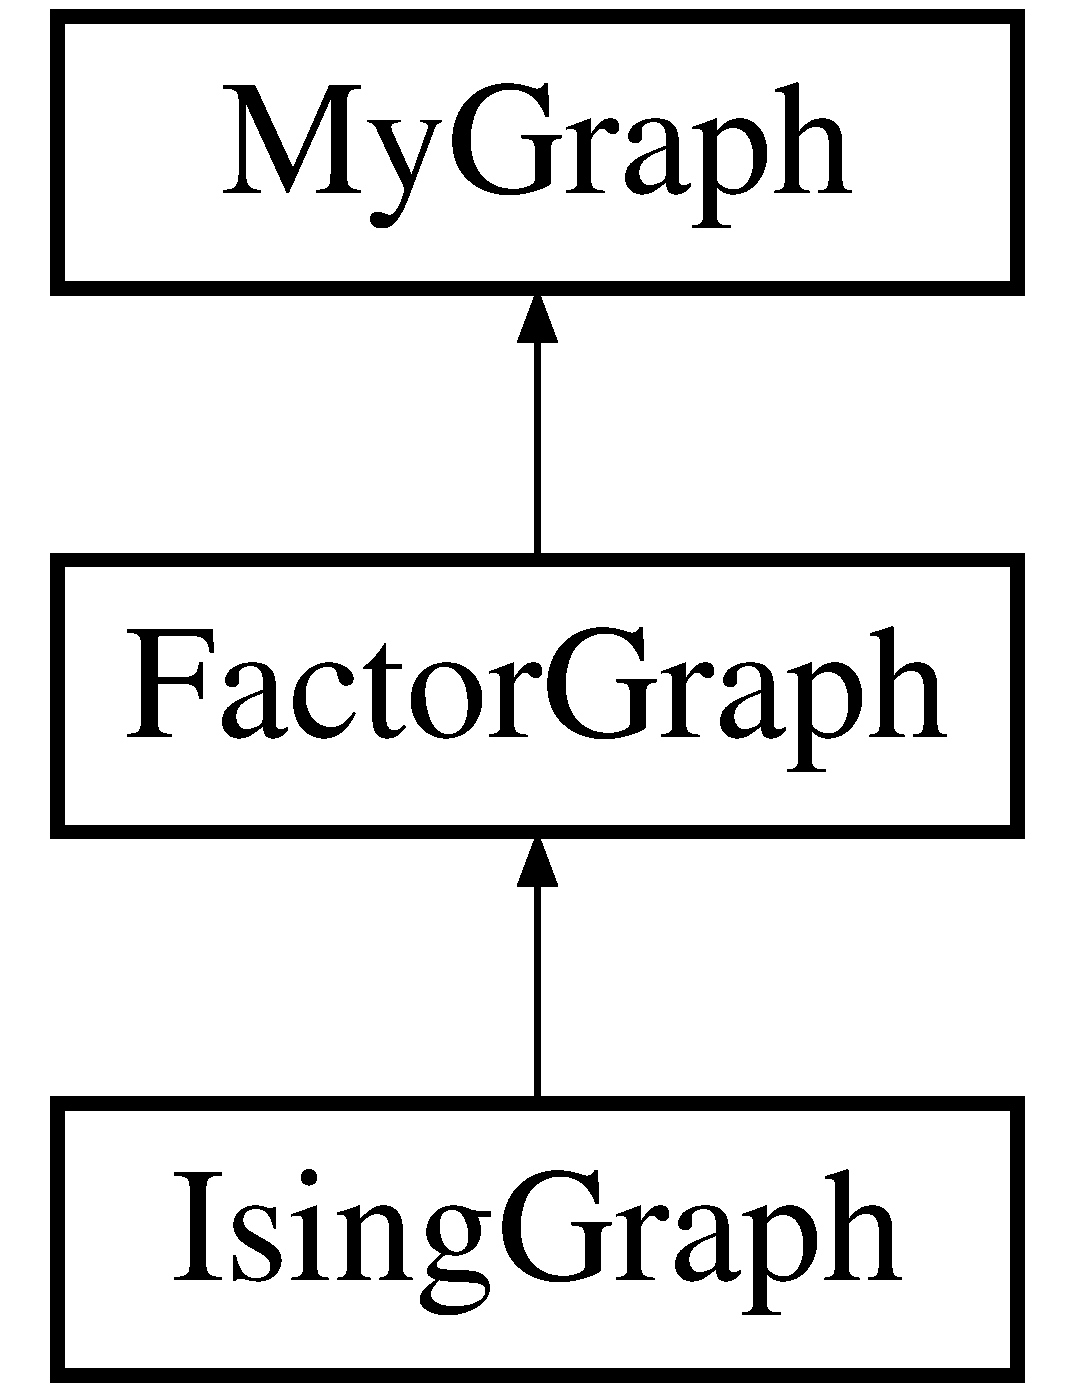
\includegraphics[height=3cm]{classIsingGraph}
\end{center}
\end{figure}
\subsection*{Public Member Functions}
\begin{CompactItemize}
\item 
{\bf IsingGraph} (int {\bf N1}, int {\bf N2}, int seed=0, {\bf LD} {\bf H\_\-sigma}=1.0, {\bf LD} {\bf J\_\-sigma}=1.0)
\item 
bool {\bf isValid} (int r, int c)
\item 
void {\bf addSpinNodes} ()
\item 
void {\bf addPairs} ()
\item 
pair$<$ int, int $>$ {\bf getGraphSize} () const
\item 
void {\bf addEdge} ({\bf NodePtr} nps, {\bf NodePtr} npt)
\item 
{\bf LD} {\bf getNodeEntropy} ({\bf NodePtr} np)
\item 
{\bf LD} {\bf getNodeEnthalpy} ({\bf NodePtr} np)
\item 
{\bf LD} {\bf getF} ()
\item 
void {\bf bp\_\-synch} (bool ch)
\item 
{\bf $\sim$IsingGraph} ()
\end{CompactItemize}
\subsection*{Private Attributes}
\begin{CompactItemize}
\item 
int {\bf N1}
\item 
int {\bf N2}
\item 
map$<$ string, {\bf LD} $>$ {\bf hMap}
\item 
map$<$ string, {\bf LD} $>$ {\bf jMap}
\item 
map$<$ string, {\bf NodePtr} $>$ {\bf npMap}
\item 
gsl\_\-rng $\ast$ {\bf myRNG}
\item 
{\bf LD} {\bf H\_\-sigma}
\item 
{\bf LD} {\bf J\_\-sigma}
\end{CompactItemize}


\subsection{Detailed Description}
Graph having the linear Ising Model Structure ( nearest neighbour interactions only ) 



\subsection{Constructor \& Destructor Documentation}
\index{IsingGraph@{IsingGraph}!IsingGraph@{IsingGraph}}
\index{IsingGraph@{IsingGraph}!IsingGraph@{IsingGraph}}
\subsubsection{\setlength{\rightskip}{0pt plus 5cm}IsingGraph::IsingGraph (int {\em N1}, int {\em N2}, int {\em seed} = {\tt 0}, {\bf LD} {\em H\_\-sigma} = {\tt 1.0}, {\bf LD} {\em J\_\-sigma} = {\tt 1.0})}\label{classIsingGraph_c244f2e67180a46a5788da77c9f9a286}


Factor graph having gaussian i.i.d. weights with nearest neighbour interactions \index{IsingGraph@{IsingGraph}!~IsingGraph@{$\sim$IsingGraph}}
\index{~IsingGraph@{$\sim$IsingGraph}!IsingGraph@{IsingGraph}}
\subsubsection{\setlength{\rightskip}{0pt plus 5cm}IsingGraph::$\sim$IsingGraph ()\hspace{0.3cm}{\tt  [inline]}}\label{classIsingGraph_e7836a9854550f380bd0c5e3a994553f}




\subsection{Member Function Documentation}
\index{IsingGraph@{IsingGraph}!isValid@{isValid}}
\index{isValid@{isValid}!IsingGraph@{IsingGraph}}
\subsubsection{\setlength{\rightskip}{0pt plus 5cm}bool IsingGraph::isValid (int {\em r}, int {\em c})}\label{classIsingGraph_65ba743b999525c4f612166d80eaced3}


\index{IsingGraph@{IsingGraph}!addSpinNodes@{addSpinNodes}}
\index{addSpinNodes@{addSpinNodes}!IsingGraph@{IsingGraph}}
\subsubsection{\setlength{\rightskip}{0pt plus 5cm}void IsingGraph::addSpinNodes ()}\label{classIsingGraph_93e844c83bf81a6418ef742569d9f11c}


Adds the spin nodes to the required graph \index{IsingGraph@{IsingGraph}!addPairs@{addPairs}}
\index{addPairs@{addPairs}!IsingGraph@{IsingGraph}}
\subsubsection{\setlength{\rightskip}{0pt plus 5cm}void IsingGraph::addPairs ()}\label{classIsingGraph_46547bdf2f5234778468ac88a7443580}


Adds the nearest neighbour interactions \index{IsingGraph@{IsingGraph}!getGraphSize@{getGraphSize}}
\index{getGraphSize@{getGraphSize}!IsingGraph@{IsingGraph}}
\subsubsection{\setlength{\rightskip}{0pt plus 5cm}pair$<$int, int$>$ IsingGraph::getGraphSize () const\hspace{0.3cm}{\tt  [inline]}}\label{classIsingGraph_40b3174a69e0b1172cd9850e9f8093a6}


\index{IsingGraph@{IsingGraph}!addEdge@{addEdge}}
\index{addEdge@{addEdge}!IsingGraph@{IsingGraph}}
\subsubsection{\setlength{\rightskip}{0pt plus 5cm}void IsingGraph::addEdge ({\bf NodePtr} {\em nps}, {\bf NodePtr} {\em npt})\hspace{0.3cm}{\tt  [inline]}}\label{classIsingGraph_fc4326bf52c5a53374659f85ba7d6f91}


\index{IsingGraph@{IsingGraph}!getNodeEntropy@{getNodeEntropy}}
\index{getNodeEntropy@{getNodeEntropy}!IsingGraph@{IsingGraph}}
\subsubsection{\setlength{\rightskip}{0pt plus 5cm}{\bf LD} IsingGraph::getNodeEntropy ({\bf NodePtr} {\em np})}\label{classIsingGraph_b85002a49e47589c9ac0d2a73efbee47}


\index{IsingGraph@{IsingGraph}!getNodeEnthalpy@{getNodeEnthalpy}}
\index{getNodeEnthalpy@{getNodeEnthalpy}!IsingGraph@{IsingGraph}}
\subsubsection{\setlength{\rightskip}{0pt plus 5cm}{\bf LD} IsingGraph::getNodeEnthalpy ({\bf NodePtr} {\em np})}\label{classIsingGraph_dc7e94d530a53e05a8ca653ee0bfde0d}


\index{IsingGraph@{IsingGraph}!getF@{getF}}
\index{getF@{getF}!IsingGraph@{IsingGraph}}
\subsubsection{\setlength{\rightskip}{0pt plus 5cm}{\bf LD} IsingGraph::getF ()}\label{classIsingGraph_435ad8bc1e11c8973b714bd3f958c54d}


\index{IsingGraph@{IsingGraph}!bp_synch@{bp\_\-synch}}
\index{bp_synch@{bp\_\-synch}!IsingGraph@{IsingGraph}}
\subsubsection{\setlength{\rightskip}{0pt plus 5cm}void IsingGraph::bp\_\-synch (bool {\em ch})}\label{classIsingGraph_599d326ae60126c24a92476b4c0affe4}




Reimplemented from {\bf FactorGraph} \doxyref{}{p.}{classFactorGraph_9cfafa8bd3ae2047576d26fb0e29c082}.

\subsection{Member Data Documentation}
\index{IsingGraph@{IsingGraph}!N1@{N1}}
\index{N1@{N1}!IsingGraph@{IsingGraph}}
\subsubsection{\setlength{\rightskip}{0pt plus 5cm}int {\bf IsingGraph::N1}\hspace{0.3cm}{\tt  [private]}}\label{classIsingGraph_609061217401524bf61e717e0ea0eebf}


\index{IsingGraph@{IsingGraph}!N2@{N2}}
\index{N2@{N2}!IsingGraph@{IsingGraph}}
\subsubsection{\setlength{\rightskip}{0pt plus 5cm}int {\bf IsingGraph::N2}\hspace{0.3cm}{\tt  [private]}}\label{classIsingGraph_7cca5baaa9d679d9406295d2f4f80cf2}


\index{IsingGraph@{IsingGraph}!hMap@{hMap}}
\index{hMap@{hMap}!IsingGraph@{IsingGraph}}
\subsubsection{\setlength{\rightskip}{0pt plus 5cm}map$<$string, {\bf LD}$>$ {\bf IsingGraph::hMap}\hspace{0.3cm}{\tt  [private]}}\label{classIsingGraph_fb247b0726431543ce64481469f4bfab}


\index{IsingGraph@{IsingGraph}!jMap@{jMap}}
\index{jMap@{jMap}!IsingGraph@{IsingGraph}}
\subsubsection{\setlength{\rightskip}{0pt plus 5cm}map$<$string, {\bf LD}$>$ {\bf IsingGraph::jMap}\hspace{0.3cm}{\tt  [private]}}\label{classIsingGraph_dd1ed6617104038eda33077ff80d0303}


\index{IsingGraph@{IsingGraph}!npMap@{npMap}}
\index{npMap@{npMap}!IsingGraph@{IsingGraph}}
\subsubsection{\setlength{\rightskip}{0pt plus 5cm}map$<$string, {\bf NodePtr}$>$ {\bf IsingGraph::npMap}\hspace{0.3cm}{\tt  [private]}}\label{classIsingGraph_86dbd5914541de872bdf2a3330b3a7b9}


\index{IsingGraph@{IsingGraph}!myRNG@{myRNG}}
\index{myRNG@{myRNG}!IsingGraph@{IsingGraph}}
\subsubsection{\setlength{\rightskip}{0pt plus 5cm}gsl\_\-rng$\ast$ {\bf IsingGraph::myRNG}\hspace{0.3cm}{\tt  [private]}}\label{classIsingGraph_235f82cd078f80ce3238bccf9b4cec75}


\index{IsingGraph@{IsingGraph}!H_sigma@{H\_\-sigma}}
\index{H_sigma@{H\_\-sigma}!IsingGraph@{IsingGraph}}
\subsubsection{\setlength{\rightskip}{0pt plus 5cm}{\bf LD} {\bf IsingGraph::H\_\-sigma}\hspace{0.3cm}{\tt  [private]}}\label{classIsingGraph_c925dc4b7f200714708c0efd5d45c874}


\index{IsingGraph@{IsingGraph}!J_sigma@{J\_\-sigma}}
\index{J_sigma@{J\_\-sigma}!IsingGraph@{IsingGraph}}
\subsubsection{\setlength{\rightskip}{0pt plus 5cm}{\bf LD} {\bf IsingGraph::J\_\-sigma}\hspace{0.3cm}{\tt  [private]}}\label{classIsingGraph_a679ca3a5702d36970ae0f18785697e3}




The documentation for this class was generated from the following files:\begin{CompactItemize}
\item 
inc/{\bf ising.h}\item 
src/{\bf ising.cpp}\end{CompactItemize}

\section{IsingRegionGraph Class Reference}
\label{classIsingRegionGraph}\index{IsingRegionGraph@{IsingRegionGraph}}
{\tt \#include $<$ising.h$>$}

Inheritance diagram for IsingRegionGraph::\begin{figure}[H]
\begin{center}
\leavevmode
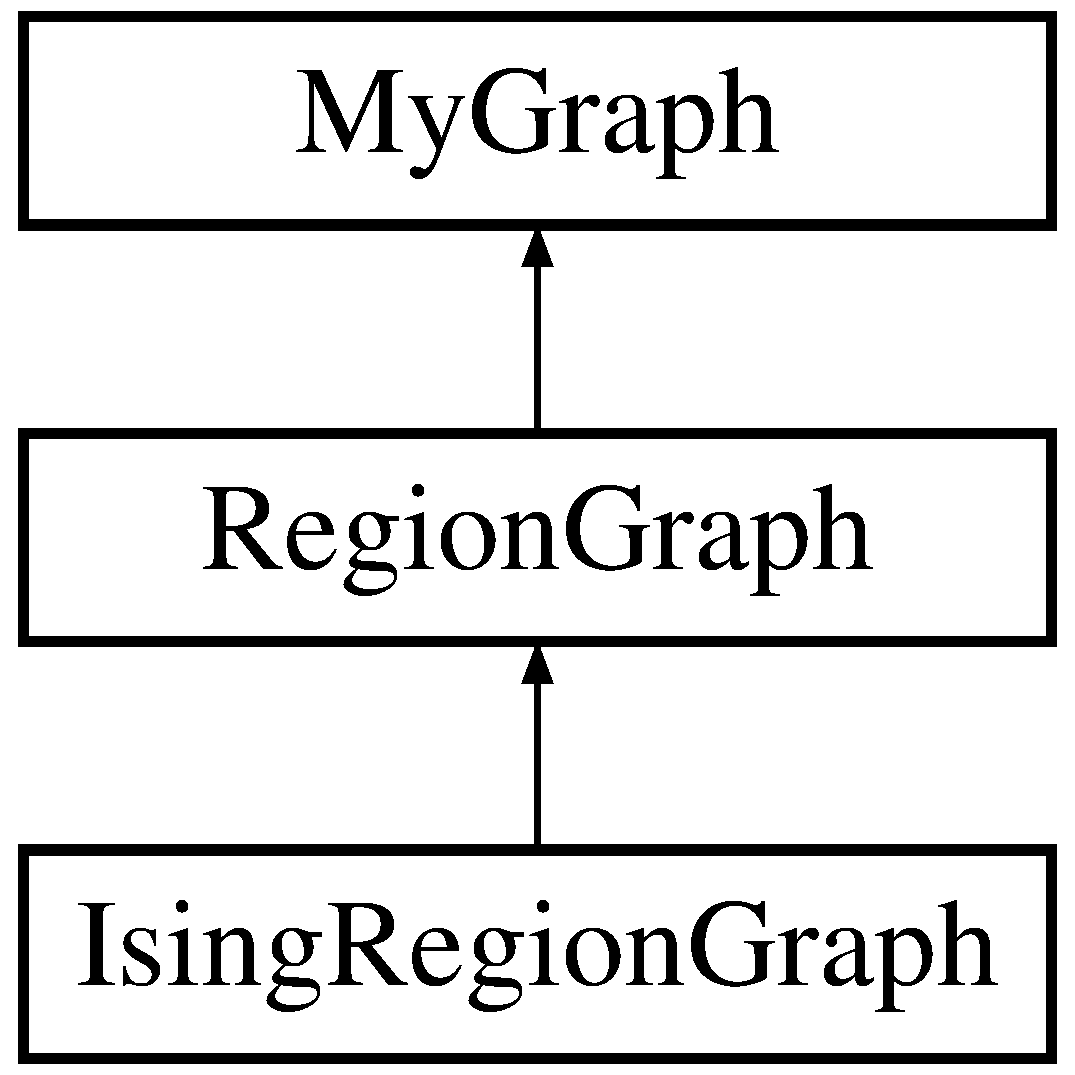
\includegraphics[height=3cm]{classIsingRegionGraph}
\end{center}
\end{figure}
\subsection*{Public Member Functions}
\begin{CompactItemize}
\item 
{\bf IsingRegionGraph} ({\bf IsingGraphPtr} graph, int \_\-rx, int \_\-ry, int \_\-cx, int \_\-cy, {\bf LD} {\bf theta}={\bf SPIN\_\-FLIP\_\-RATE}, {\bf LD} {\bf delta\_\-t}={\bf DELTA\_\-T})
\item 
bool {\bf isValid} (int r, int c)
\item 
{\bf Cluster} {\bf genMaximalRegion} (int x, int y)
\item 
void {\bf genSubRegions} ()
\item 
void {\bf initEdgeMsgs} (pair$<$ {\bf EdgePtr}, {\bf EdgePtr} $>$ ep)
\begin{CompactList}\small\item\em initialize the messages as given \item\end{CompactList}\item 
{\bf LD} {\bf getPrntM} (const {\bf RegionPtr} \&rp, const {\bf StatePtr} \&sp)
\item 
{\bf LD} {\bf getChldM} (const {\bf RegionPtr} \&rp, const {\bf StatePtr} \&sp0, const {\bf StatePtr} \&spT)
\item 
{\bf LD} {\bf getPrntM} (const {\bf RegionPtr} \&rp, const {\bf StatePtr} \&sp0, const {\bf StatePtr} \&spT)
\item 
{\bf ConditionalBeliefPtr} {\bf getCondBlfForRegn} ({\bf Region} $\ast$np)
\begin{CompactList}\small\item\em this gives the conditional P(x\_\-0 $|$ x\_\-dt) for the region \item\end{CompactList}\item 
void {\bf initBeliefs} ({\bf RegionPtr} \&rp)
\item 
void {\bf updateZ} ({\bf RegionPtr} \&rp)
\item 
{\bf LD} {\bf updateB\_\-t\_\-0} ({\bf RegionPtr} \&rp)
\begin{CompactList}\small\item\em returns the maximum change relative \item\end{CompactList}\item 
{\bf LD} {\bf updateB\_\-t} ({\bf RegionPtr} \&rp)
\item 
{\bf LD} {\bf getMsgCtoP} ({\bf EdgePtr} e, {\bf StatePtr} s0, {\bf StatePtr} sT)
\item 
bool {\bf bp\_\-ppm} ({\bf LD} \_\-th={\bf SPIN\_\-FLIP\_\-RATE}, {\bf LD} \_\-delta\_\-t={\bf DELTA\_\-T})
\item 
pair$<$ {\bf LD}, {\bf LD} $>$ {\bf update\_\-edges} ({\bf LD} cFactor=1.0)
\item 
{\bf LD} {\bf getMargPr} (const {\bf RegionPtr} \&rp, string var)
\item 
{\bf LD} {\bf getF} ()
\item 
bool {\bf renormalizeMessages} (pair$<$ {\bf LD}, {\bf LD} $>$ maxMinMsgPair, {\bf LD} lmt=1.0)
\item 
bool {\bf ppm\_\-iter} ({\bf LD} \_\-th, {\bf LD} \_\-delta\_\-t, {\bf LD} $\ast$minMsg, {\bf LD} $\ast$maxMsg, {\bf LD} $\ast$maxDev, {\bf LD} $\ast$avgDev, map$<$ string, vector$<$ {\bf LD} $>$ $>$ $\ast$nextBlfMpPtr=0, {\bf LD} lmt=1.0)
\end{CompactItemize}
\subsection*{Private Attributes}
\begin{CompactItemize}
\item 
{\bf IsingGraphPtr} {\bf graphPtr}
\begin{CompactList}\small\item\em original ising graph \item\end{CompactList}\item 
int {\bf rx}
\begin{CompactList}\small\item\em biggest region width \item\end{CompactList}\item 
int {\bf ry}
\begin{CompactList}\small\item\em biggest region size \item\end{CompactList}\item 
int {\bf cx}
\begin{CompactList}\small\item\em how much x-overlap between current and next region \item\end{CompactList}\item 
int {\bf cy}
\begin{CompactList}\small\item\em how much y-overlap between current and next region \item\end{CompactList}\item 
int {\bf N1}
\begin{CompactList}\small\item\em how many rows \item\end{CompactList}\item 
int {\bf N2}
\begin{CompactList}\small\item\em how many columns \item\end{CompactList}\item 
map$<$ {\bf Cluster}, int, {\bf ClusterCmp} $>$ {\bf clusters}
\begin{CompactList}\small\item\em the clustering given by genMaximalRegions along with counting numbers \item\end{CompactList}\item 
{\bf LD} {\bf theta}
\begin{CompactList}\small\item\em spin flip rate \item\end{CompactList}\item 
{\bf LD} {\bf delta\_\-t}
\begin{CompactList}\small\item\em the time of simulation \item\end{CompactList}\item 
int {\bf iterNum}
\begin{CompactList}\small\item\em iteration count \item\end{CompactList}\end{CompactItemize}


\subsection{Constructor \& Destructor Documentation}
\index{IsingRegionGraph@{IsingRegionGraph}!IsingRegionGraph@{IsingRegionGraph}}
\index{IsingRegionGraph@{IsingRegionGraph}!IsingRegionGraph@{IsingRegionGraph}}
\subsubsection{\setlength{\rightskip}{0pt plus 5cm}IsingRegionGraph::IsingRegionGraph ({\bf IsingGraphPtr} {\em graph}, int {\em \_\-rx}, int {\em \_\-ry}, int {\em \_\-cx}, int {\em \_\-cy}, {\bf LD} {\em \_\-theta} = {\tt {\bf SPIN\_\-FLIP\_\-RATE}}, {\bf LD} {\em \_\-delta\_\-t} = {\tt {\bf DELTA\_\-T}})}\label{classIsingRegionGraph_c76abee7ef1427e1cfb4c0180087a9eb}


\doxyref{Region}{p.}{classRegion} graph based on the underlying ising graph 

\subsection{Member Function Documentation}
\index{IsingRegionGraph@{IsingRegionGraph}!isValid@{isValid}}
\index{isValid@{isValid}!IsingRegionGraph@{IsingRegionGraph}}
\subsubsection{\setlength{\rightskip}{0pt plus 5cm}bool IsingRegionGraph::isValid (int {\em r}, int {\em c})\hspace{0.3cm}{\tt  [inline]}}\label{classIsingRegionGraph_171908138a5f81b830d576721dc6b03a}


\index{IsingRegionGraph@{IsingRegionGraph}!genMaximalRegion@{genMaximalRegion}}
\index{genMaximalRegion@{genMaximalRegion}!IsingRegionGraph@{IsingRegionGraph}}
\subsubsection{\setlength{\rightskip}{0pt plus 5cm}{\bf Cluster} IsingRegionGraph::genMaximalRegion (int {\em x}, int {\em y})}\label{classIsingRegionGraph_6f60c52fa606b8b36236c91c2b66e36a}


Generate the maximal regions \index{IsingRegionGraph@{IsingRegionGraph}!genSubRegions@{genSubRegions}}
\index{genSubRegions@{genSubRegions}!IsingRegionGraph@{IsingRegionGraph}}
\subsubsection{\setlength{\rightskip}{0pt plus 5cm}void IsingRegionGraph::genSubRegions ()}\label{classIsingRegionGraph_233891cd079d1535ca9635f04f52b62b}


\index{IsingRegionGraph@{IsingRegionGraph}!initEdgeMsgs@{initEdgeMsgs}}
\index{initEdgeMsgs@{initEdgeMsgs}!IsingRegionGraph@{IsingRegionGraph}}
\subsubsection{\setlength{\rightskip}{0pt plus 5cm}void IsingRegionGraph::initEdgeMsgs (pair$<$ {\bf EdgePtr}, {\bf EdgePtr} $>$ {\em ep})}\label{classIsingRegionGraph_e4996023cc225d3ae71afbff4ef4da6b}


initialize the messages as given 

\index{IsingRegionGraph@{IsingRegionGraph}!getPrntM@{getPrntM}}
\index{getPrntM@{getPrntM}!IsingRegionGraph@{IsingRegionGraph}}
\subsubsection{\setlength{\rightskip}{0pt plus 5cm}{\bf LD} IsingRegionGraph::getPrntM (const {\bf RegionPtr} \& {\em rp}, const {\bf StatePtr} \& {\em sp})}\label{classIsingRegionGraph_fa42d579cb9caad880c225187c1e2ab8}


\index{IsingRegionGraph@{IsingRegionGraph}!getChldM@{getChldM}}
\index{getChldM@{getChldM}!IsingRegionGraph@{IsingRegionGraph}}
\subsubsection{\setlength{\rightskip}{0pt plus 5cm}{\bf LD} IsingRegionGraph::getChldM (const {\bf RegionPtr} \& {\em rp}, const {\bf StatePtr} \& {\em sp0}, const {\bf StatePtr} \& {\em spT})}\label{classIsingRegionGraph_92d4116cbbe3dedd600d0913dd46c646}


\index{IsingRegionGraph@{IsingRegionGraph}!getPrntM@{getPrntM}}
\index{getPrntM@{getPrntM}!IsingRegionGraph@{IsingRegionGraph}}
\subsubsection{\setlength{\rightskip}{0pt plus 5cm}{\bf LD} IsingRegionGraph::getPrntM (const {\bf RegionPtr} \& {\em rp}, const {\bf StatePtr} \& {\em sp0}, const {\bf StatePtr} \& {\em spT})}\label{classIsingRegionGraph_1ba8e199f9eaaf291a5ec5e3972ec2fb}


\index{IsingRegionGraph@{IsingRegionGraph}!getCondBlfForRegn@{getCondBlfForRegn}}
\index{getCondBlfForRegn@{getCondBlfForRegn}!IsingRegionGraph@{IsingRegionGraph}}
\subsubsection{\setlength{\rightskip}{0pt plus 5cm}{\bf ConditionalBeliefPtr} IsingRegionGraph::getCondBlfForRegn ({\bf Region} $\ast$ {\em np})}\label{classIsingRegionGraph_bcd3adcf36b489e20cba3c52806bd84b}


this gives the conditional P(x\_\-0 $|$ x\_\-dt) for the region 

\index{IsingRegionGraph@{IsingRegionGraph}!initBeliefs@{initBeliefs}}
\index{initBeliefs@{initBeliefs}!IsingRegionGraph@{IsingRegionGraph}}
\subsubsection{\setlength{\rightskip}{0pt plus 5cm}void IsingRegionGraph::initBeliefs ({\bf RegionPtr} \& {\em rp})}\label{classIsingRegionGraph_04dc9a6b8f484c0c66a085b3bcc482c0}


\index{IsingRegionGraph@{IsingRegionGraph}!updateZ@{updateZ}}
\index{updateZ@{updateZ}!IsingRegionGraph@{IsingRegionGraph}}
\subsubsection{\setlength{\rightskip}{0pt plus 5cm}void IsingRegionGraph::updateZ ({\bf RegionPtr} \& {\em rp})}\label{classIsingRegionGraph_367a0175852f4ba650080455a2a8decd}


\index{IsingRegionGraph@{IsingRegionGraph}!updateB_t_0@{updateB\_\-t\_\-0}}
\index{updateB_t_0@{updateB\_\-t\_\-0}!IsingRegionGraph@{IsingRegionGraph}}
\subsubsection{\setlength{\rightskip}{0pt plus 5cm}{\bf LD} IsingRegionGraph::updateB\_\-t\_\-0 ({\bf RegionPtr} \& {\em rp})}\label{classIsingRegionGraph_81248762014c897d84f8664d40324a07}


returns the maximum change relative 

\index{IsingRegionGraph@{IsingRegionGraph}!updateB_t@{updateB\_\-t}}
\index{updateB_t@{updateB\_\-t}!IsingRegionGraph@{IsingRegionGraph}}
\subsubsection{\setlength{\rightskip}{0pt plus 5cm}{\bf LD} IsingRegionGraph::updateB\_\-t ({\bf RegionPtr} \& {\em rp})\hspace{0.3cm}{\tt  [inline]}}\label{classIsingRegionGraph_8587913d2830f3a3bf07f4577fd06be0}


\index{IsingRegionGraph@{IsingRegionGraph}!getMsgCtoP@{getMsgCtoP}}
\index{getMsgCtoP@{getMsgCtoP}!IsingRegionGraph@{IsingRegionGraph}}
\subsubsection{\setlength{\rightskip}{0pt plus 5cm}{\bf LD} IsingRegionGraph::getMsgCtoP ({\bf EdgePtr} {\em e}, {\bf StatePtr} {\em s0}, {\bf StatePtr} {\em sT})}\label{classIsingRegionGraph_28d286abd1085a1c815e9f6e43277a0b}


\index{IsingRegionGraph@{IsingRegionGraph}!bp_ppm@{bp\_\-ppm}}
\index{bp_ppm@{bp\_\-ppm}!IsingRegionGraph@{IsingRegionGraph}}
\subsubsection{\setlength{\rightskip}{0pt plus 5cm}bool IsingRegionGraph::bp\_\-ppm ({\bf LD} {\em \_\-th} = {\tt {\bf SPIN\_\-FLIP\_\-RATE}}, {\bf LD} {\em \_\-delta\_\-t} = {\tt {\bf DELTA\_\-T}})}\label{classIsingRegionGraph_0d6c04b81a9026af9aa8aba9ba38e43b}


\index{IsingRegionGraph@{IsingRegionGraph}!update_edges@{update\_\-edges}}
\index{update_edges@{update\_\-edges}!IsingRegionGraph@{IsingRegionGraph}}
\subsubsection{\setlength{\rightskip}{0pt plus 5cm}pair$<$ {\bf LD}, {\bf LD} $>$ IsingRegionGraph::update\_\-edges ({\bf LD} {\em cFactor} = {\tt 1.0})}\label{classIsingRegionGraph_d085863bdad4c66f8abb20ba0e52be58}


\index{IsingRegionGraph@{IsingRegionGraph}!getMargPr@{getMargPr}}
\index{getMargPr@{getMargPr}!IsingRegionGraph@{IsingRegionGraph}}
\subsubsection{\setlength{\rightskip}{0pt plus 5cm}{\bf LD} IsingRegionGraph::getMargPr (const {\bf RegionPtr} \& {\em rp}, string {\em var})}\label{classIsingRegionGraph_e6846f3dd2551218ad41149be6672e43}


\index{IsingRegionGraph@{IsingRegionGraph}!getF@{getF}}
\index{getF@{getF}!IsingRegionGraph@{IsingRegionGraph}}
\subsubsection{\setlength{\rightskip}{0pt plus 5cm}{\bf LD} IsingRegionGraph::getF ()}\label{classIsingRegionGraph_7dc186f4bd321af087fb6b99b3e80b59}


\index{IsingRegionGraph@{IsingRegionGraph}!renormalizeMessages@{renormalizeMessages}}
\index{renormalizeMessages@{renormalizeMessages}!IsingRegionGraph@{IsingRegionGraph}}
\subsubsection{\setlength{\rightskip}{0pt plus 5cm}bool IsingRegionGraph::renormalizeMessages (pair$<$ {\bf LD}, {\bf LD} $>$ {\em maxMinMsgPair}, {\bf LD} {\em lmt} = {\tt 1.0})}\label{classIsingRegionGraph_95e68069fee6452b609dd2797853e0df}


\index{IsingRegionGraph@{IsingRegionGraph}!ppm_iter@{ppm\_\-iter}}
\index{ppm_iter@{ppm\_\-iter}!IsingRegionGraph@{IsingRegionGraph}}
\subsubsection{\setlength{\rightskip}{0pt plus 5cm}bool IsingRegionGraph::ppm\_\-iter ({\bf LD} {\em \_\-th}, {\bf LD} {\em \_\-delta\_\-t}, {\bf LD} $\ast$ {\em minMsg}, {\bf LD} $\ast$ {\em maxMsg}, {\bf LD} $\ast$ {\em maxDev}, {\bf LD} $\ast$ {\em avgDev}, map$<$ string, vector$<$ {\bf LD} $>$ $>$ $\ast$ {\em nextBlfMpPtr} = {\tt 0}, {\bf LD} {\em lmt} = {\tt 1.0})}\label{classIsingRegionGraph_cb517e32f07bbf17ff637df24eaab54b}




\subsection{Member Data Documentation}
\index{IsingRegionGraph@{IsingRegionGraph}!graphPtr@{graphPtr}}
\index{graphPtr@{graphPtr}!IsingRegionGraph@{IsingRegionGraph}}
\subsubsection{\setlength{\rightskip}{0pt plus 5cm}{\bf IsingGraphPtr} {\bf IsingRegionGraph::graphPtr}\hspace{0.3cm}{\tt  [private]}}\label{classIsingRegionGraph_66bffb3f21f7597e2dfa5027eae7d7e8}


original ising graph 



Reimplemented from {\bf RegionGraph} \doxyref{}{p.}{classRegionGraph_7dad8406a69860b74ab83e3153cf57ac}.\index{IsingRegionGraph@{IsingRegionGraph}!rx@{rx}}
\index{rx@{rx}!IsingRegionGraph@{IsingRegionGraph}}
\subsubsection{\setlength{\rightskip}{0pt plus 5cm}int {\bf IsingRegionGraph::rx}\hspace{0.3cm}{\tt  [private]}}\label{classIsingRegionGraph_966c1b2fa298435ffb293650e899f6d7}


biggest region width 

\index{IsingRegionGraph@{IsingRegionGraph}!ry@{ry}}
\index{ry@{ry}!IsingRegionGraph@{IsingRegionGraph}}
\subsubsection{\setlength{\rightskip}{0pt plus 5cm}int {\bf IsingRegionGraph::ry}\hspace{0.3cm}{\tt  [private]}}\label{classIsingRegionGraph_350ad0f15dbbbb4246fdfb0f43f3b397}


biggest region size 

\index{IsingRegionGraph@{IsingRegionGraph}!cx@{cx}}
\index{cx@{cx}!IsingRegionGraph@{IsingRegionGraph}}
\subsubsection{\setlength{\rightskip}{0pt plus 5cm}int {\bf IsingRegionGraph::cx}\hspace{0.3cm}{\tt  [private]}}\label{classIsingRegionGraph_8ca48f88be4e6654875574fd08d1fb26}


how much x-overlap between current and next region 

\index{IsingRegionGraph@{IsingRegionGraph}!cy@{cy}}
\index{cy@{cy}!IsingRegionGraph@{IsingRegionGraph}}
\subsubsection{\setlength{\rightskip}{0pt plus 5cm}int {\bf IsingRegionGraph::cy}\hspace{0.3cm}{\tt  [private]}}\label{classIsingRegionGraph_34b3917e86813a7677ed3d20fd99bd24}


how much y-overlap between current and next region 

\index{IsingRegionGraph@{IsingRegionGraph}!N1@{N1}}
\index{N1@{N1}!IsingRegionGraph@{IsingRegionGraph}}
\subsubsection{\setlength{\rightskip}{0pt plus 5cm}int {\bf IsingRegionGraph::N1}\hspace{0.3cm}{\tt  [private]}}\label{classIsingRegionGraph_1a0d0c44550a4ec10c4b6b6a343ee96c}


how many rows 

\index{IsingRegionGraph@{IsingRegionGraph}!N2@{N2}}
\index{N2@{N2}!IsingRegionGraph@{IsingRegionGraph}}
\subsubsection{\setlength{\rightskip}{0pt plus 5cm}int {\bf IsingRegionGraph::N2}\hspace{0.3cm}{\tt  [private]}}\label{classIsingRegionGraph_3c584fb5f3686133a777a864bdfcbf5c}


how many columns 

\index{IsingRegionGraph@{IsingRegionGraph}!clusters@{clusters}}
\index{clusters@{clusters}!IsingRegionGraph@{IsingRegionGraph}}
\subsubsection{\setlength{\rightskip}{0pt plus 5cm}map$<${\bf Cluster}, int, {\bf ClusterCmp}$>$ {\bf IsingRegionGraph::clusters}\hspace{0.3cm}{\tt  [private]}}\label{classIsingRegionGraph_50a06c5da423fe62fe9f492f2f3e4c06}


the clustering given by genMaximalRegions along with counting numbers 

\index{IsingRegionGraph@{IsingRegionGraph}!theta@{theta}}
\index{theta@{theta}!IsingRegionGraph@{IsingRegionGraph}}
\subsubsection{\setlength{\rightskip}{0pt plus 5cm}{\bf LD} {\bf IsingRegionGraph::theta}\hspace{0.3cm}{\tt  [private]}}\label{classIsingRegionGraph_6365d9f865232ccdb18c1cb6e604943e}


spin flip rate 

\index{IsingRegionGraph@{IsingRegionGraph}!delta_t@{delta\_\-t}}
\index{delta_t@{delta\_\-t}!IsingRegionGraph@{IsingRegionGraph}}
\subsubsection{\setlength{\rightskip}{0pt plus 5cm}{\bf LD} {\bf IsingRegionGraph::delta\_\-t}\hspace{0.3cm}{\tt  [private]}}\label{classIsingRegionGraph_751c6177f82d866e4b617e99e2fdff9b}


the time of simulation 

\index{IsingRegionGraph@{IsingRegionGraph}!iterNum@{iterNum}}
\index{iterNum@{iterNum}!IsingRegionGraph@{IsingRegionGraph}}
\subsubsection{\setlength{\rightskip}{0pt plus 5cm}int {\bf IsingRegionGraph::iterNum}\hspace{0.3cm}{\tt  [private]}}\label{classIsingRegionGraph_119748dee2fe786616d77cb4ab2e1535}


iteration count 



The documentation for this class was generated from the following files:\begin{CompactItemize}
\item 
inc/{\bf ising.h}\item 
src/{\bf ising.cpp}\end{CompactItemize}

\section{ModelMVI Class Reference}
\label{classModelMVI}\index{ModelMVI@{ModelMVI}}
{\tt \#include $<$MVI.h$>$}

Inheritance diagram for ModelMVI::\begin{figure}[H]
\begin{center}
\leavevmode
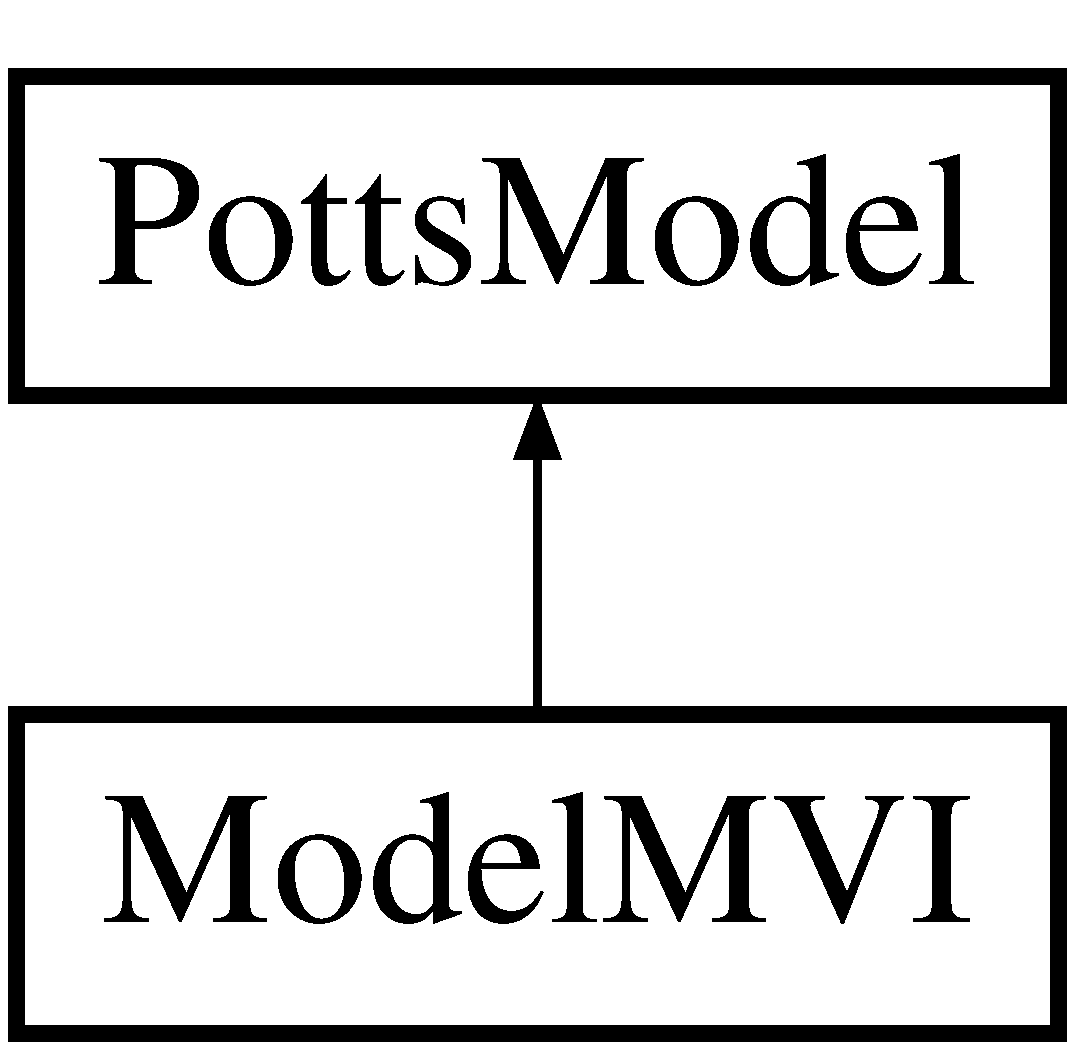
\includegraphics[height=2cm]{classModelMVI}
\end{center}
\end{figure}
\subsection*{Public Member Functions}
\begin{CompactItemize}
\item 
{\bf ModelMVI} (int {\bf N1}, int {\bf N2}, int {\bf Q})
\item 
{\bf LD} {\bf getP} (string fid, {\bf StatePtr} sC)
\end{CompactItemize}


\subsection{Constructor \& Destructor Documentation}
\index{ModelMVI@{ModelMVI}!ModelMVI@{ModelMVI}}
\index{ModelMVI@{ModelMVI}!ModelMVI@{ModelMVI}}
\subsubsection{\setlength{\rightskip}{0pt plus 5cm}ModelMVI::ModelMVI (int {\em N1}, int {\em N2}, int {\em Q})\hspace{0.3cm}{\tt  [inline]}}\label{classModelMVI_23b4348c8e6bb3ac8a30451666e4bcb3}




\subsection{Member Function Documentation}
\index{ModelMVI@{ModelMVI}!getP@{getP}}
\index{getP@{getP}!ModelMVI@{ModelMVI}}
\subsubsection{\setlength{\rightskip}{0pt plus 5cm}{\bf LD} ModelMVI::getP (string {\em fid}, {\bf StatePtr} {\em sC})\hspace{0.3cm}{\tt  [inline]}}\label{classModelMVI_c65577d0b71f762361c063d82e84e478}




Reimplemented from {\bf PottsModel} \doxyref{}{p.}{structPottsModel_ccd5dfd6de009b38b8689be20d04c55f}.

The documentation for this class was generated from the following file:\begin{CompactItemize}
\item 
inc/{\bf MVI.h}\end{CompactItemize}

\section{MVI Class Reference}
\label{classMVI}\index{MVI@{MVI}}
{\tt \#include $<$MVI.h$>$}

\subsection*{Public Member Functions}
\begin{CompactItemize}
\item 
{\bf MVI} (string \_\-fname, int \_\-Q\_\-potts=4, {\bf LD} \_\-TR=0.7, {\bf LD} \_\-TT=0.7)
\item 
void {\bf init} ()
\item 
int {\bf run} (bool ppm=true, int numLow=0)
\end{CompactItemize}
\subsection*{Private Attributes}
\begin{CompactItemize}
\item 
int {\bf N1}
\item 
int {\bf N2}
\item 
int {\bf Q\_\-potts}
\item 
{\bf LD} {\bf TR}
\item 
{\bf LD} {\bf TT}
\item 
string {\bf fname}
\item 
{\bf VR} $\ast$ {\bf vr}
\item 
{\bf GraphMVI} $\ast$ {\bf graph}
\item 
{\bf ModelMVI} $\ast$ {\bf model}
\end{CompactItemize}


\subsection{Constructor \& Destructor Documentation}
\index{MVI@{MVI}!MVI@{MVI}}
\index{MVI@{MVI}!MVI@{MVI}}
\subsubsection{\setlength{\rightskip}{0pt plus 5cm}MVI::MVI (string {\em \_\-fname}, int {\em \_\-Q\_\-potts} = {\tt 4}, {\bf LD} {\em \_\-TR} = {\tt 0.7}, {\bf LD} {\em \_\-TT} = {\tt 0.7})\hspace{0.3cm}{\tt  [inline]}}\label{classMVI_16d5d4ef417c5a8c29d36aab7522301f}




\subsection{Member Function Documentation}
\index{MVI@{MVI}!init@{init}}
\index{init@{init}!MVI@{MVI}}
\subsubsection{\setlength{\rightskip}{0pt plus 5cm}void MVI::init ()}\label{classMVI_fbf8f75717db65cc9f8e0d7ce51e2534}


\index{MVI@{MVI}!run@{run}}
\index{run@{run}!MVI@{MVI}}
\subsubsection{\setlength{\rightskip}{0pt plus 5cm}int MVI::run (bool {\em ppm} = {\tt true}, int {\em numLow} = {\tt 0})}\label{classMVI_dcd50473c7f80b742cd7001dcb85e89b}




\subsection{Member Data Documentation}
\index{MVI@{MVI}!N1@{N1}}
\index{N1@{N1}!MVI@{MVI}}
\subsubsection{\setlength{\rightskip}{0pt plus 5cm}int {\bf MVI::N1}\hspace{0.3cm}{\tt  [private]}}\label{classMVI_fc91264ae571653d735c76761a3f00ef}


\index{MVI@{MVI}!N2@{N2}}
\index{N2@{N2}!MVI@{MVI}}
\subsubsection{\setlength{\rightskip}{0pt plus 5cm}int {\bf MVI::N2}\hspace{0.3cm}{\tt  [private]}}\label{classMVI_7d978b290f957a8de231ab3876b564c1}


\index{MVI@{MVI}!Q_potts@{Q\_\-potts}}
\index{Q_potts@{Q\_\-potts}!MVI@{MVI}}
\subsubsection{\setlength{\rightskip}{0pt plus 5cm}int {\bf MVI::Q\_\-potts}\hspace{0.3cm}{\tt  [private]}}\label{classMVI_fc77b5ea4a4e4e911f9e75da72219dd2}


\index{MVI@{MVI}!TR@{TR}}
\index{TR@{TR}!MVI@{MVI}}
\subsubsection{\setlength{\rightskip}{0pt plus 5cm}{\bf LD} {\bf MVI::TR}\hspace{0.3cm}{\tt  [private]}}\label{classMVI_ed3c60c55124dcc33cd2c7f8a9eb4b68}


\index{MVI@{MVI}!TT@{TT}}
\index{TT@{TT}!MVI@{MVI}}
\subsubsection{\setlength{\rightskip}{0pt plus 5cm}{\bf LD} {\bf MVI::TT}\hspace{0.3cm}{\tt  [private]}}\label{classMVI_3d425fad2d288ddcfc1123cec728ca45}


\index{MVI@{MVI}!fname@{fname}}
\index{fname@{fname}!MVI@{MVI}}
\subsubsection{\setlength{\rightskip}{0pt plus 5cm}string {\bf MVI::fname}\hspace{0.3cm}{\tt  [private]}}\label{classMVI_03b414b2878a3bd9f404b9eb6ca4d9c0}


\index{MVI@{MVI}!vr@{vr}}
\index{vr@{vr}!MVI@{MVI}}
\subsubsection{\setlength{\rightskip}{0pt plus 5cm}{\bf VR}$\ast$ {\bf MVI::vr}\hspace{0.3cm}{\tt  [private]}}\label{classMVI_eb6c1bf8a6f2fc713574ff2e351bff58}


\index{MVI@{MVI}!graph@{graph}}
\index{graph@{graph}!MVI@{MVI}}
\subsubsection{\setlength{\rightskip}{0pt plus 5cm}{\bf GraphMVI}$\ast$ {\bf MVI::graph}\hspace{0.3cm}{\tt  [private]}}\label{classMVI_2d1b3fefaa2dcc0dbdb059f739479fd7}


\index{MVI@{MVI}!model@{model}}
\index{model@{model}!MVI@{MVI}}
\subsubsection{\setlength{\rightskip}{0pt plus 5cm}{\bf ModelMVI}$\ast$ {\bf MVI::model}\hspace{0.3cm}{\tt  [private]}}\label{classMVI_d7e7496b16b254e6044d4fd04efd2c9c}




The documentation for this class was generated from the following files:\begin{CompactItemize}
\item 
inc/{\bf MVI.h}\item 
src/{\bf MVI.cpp}\end{CompactItemize}

\section{MyEdge Struct Reference}
\label{structMyEdge}\index{MyEdge@{MyEdge}}
{\tt \#include $<$myedge.h$>$}

\subsection*{Public Member Functions}
\begin{CompactItemize}
\item 
{\bf MyEdge} ({\bf NodePtr} n1, {\bf NodePtr} n2)
\item 
{\bf LD} {\bf getMsg} ({\bf StatePtr} val)
\item 
void {\bf setMsg} ({\bf StatePtr} val, {\bf LD} d)
\end{CompactItemize}
\subsection*{Public Attributes}
\begin{CompactItemize}
\item 
{\bf NodePtr} {\bf ends} [2]
\item 
map$<$ {\bf StatePtr}, {\bf LD}, {\bf StatePtrCmp} $>$ {\bf msgMp}
\end{CompactItemize}
\subsection*{Friends}
\begin{CompactItemize}
\item 
ostream \& {\bf operator$<$$<$} (ostream \&os, {\bf MyEdge} \&e)
\end{CompactItemize}


\subsection{Constructor \& Destructor Documentation}
\index{MyEdge@{MyEdge}!MyEdge@{MyEdge}}
\index{MyEdge@{MyEdge}!MyEdge@{MyEdge}}
\subsubsection{\setlength{\rightskip}{0pt plus 5cm}MyEdge::MyEdge ({\bf NodePtr} {\em n1}, {\bf NodePtr} {\em n2})\hspace{0.3cm}{\tt  [inline]}}\label{structMyEdge_b7915fe8b92575e5828d658f3b362310}




\subsection{Member Function Documentation}
\index{MyEdge@{MyEdge}!getMsg@{getMsg}}
\index{getMsg@{getMsg}!MyEdge@{MyEdge}}
\subsubsection{\setlength{\rightskip}{0pt plus 5cm}{\bf LD} MyEdge::getMsg ({\bf StatePtr} {\em val})\hspace{0.3cm}{\tt  [inline]}}\label{structMyEdge_9e32cab50a3f3bfc2e362f2f1943af4a}


\index{MyEdge@{MyEdge}!setMsg@{setMsg}}
\index{setMsg@{setMsg}!MyEdge@{MyEdge}}
\subsubsection{\setlength{\rightskip}{0pt plus 5cm}void MyEdge::setMsg ({\bf StatePtr} {\em val}, {\bf LD} {\em d})\hspace{0.3cm}{\tt  [inline]}}\label{structMyEdge_e0889d6843138a8782cb8b70516a8301}




\subsection{Friends And Related Function Documentation}
\index{MyEdge@{MyEdge}!operator<<@{operator$<$$<$}}
\index{operator<<@{operator$<$$<$}!MyEdge@{MyEdge}}
\subsubsection{\setlength{\rightskip}{0pt plus 5cm}ostream\& operator$<$$<$ (ostream \& {\em os}, {\bf MyEdge} \& {\em e})\hspace{0.3cm}{\tt  [friend]}}\label{structMyEdge_62df515d472be9c0e91bd9f5350a7675}




\subsection{Member Data Documentation}
\index{MyEdge@{MyEdge}!ends@{ends}}
\index{ends@{ends}!MyEdge@{MyEdge}}
\subsubsection{\setlength{\rightskip}{0pt plus 5cm}{\bf NodePtr} {\bf MyEdge::ends}[2]}\label{structMyEdge_b6fb1f7eaa15a3136087c8551f9ce8d6}


\index{MyEdge@{MyEdge}!msgMp@{msgMp}}
\index{msgMp@{msgMp}!MyEdge@{MyEdge}}
\subsubsection{\setlength{\rightskip}{0pt plus 5cm}map$<${\bf StatePtr}, {\bf LD}, {\bf StatePtrCmp}$>$ {\bf MyEdge::msgMp}}\label{structMyEdge_2d2cab4963ddfcadd6cc05ab225b8ff2}




The documentation for this struct was generated from the following file:\begin{CompactItemize}
\item 
inc/{\bf myedge.h}\end{CompactItemize}

\section{MyGraph Class Reference}
\label{classMyGraph}\index{MyGraph@{MyGraph}}
{\tt \#include $<$mygraph.h$>$}

Inheritance diagram for MyGraph::\begin{figure}[H]
\begin{center}
\leavevmode
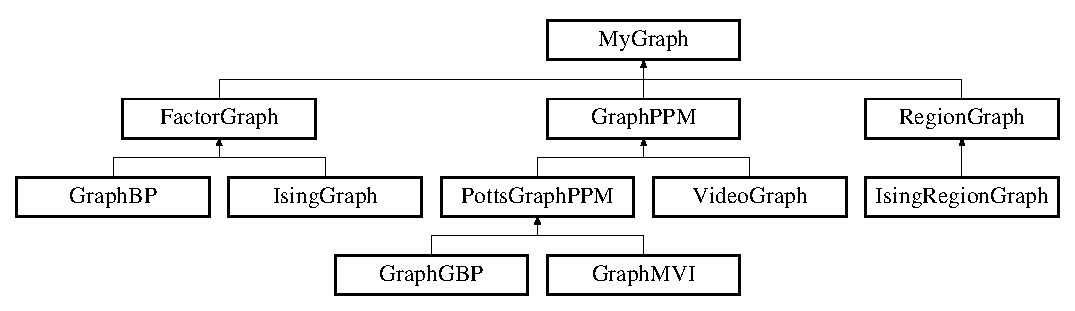
\includegraphics[height=3.73333cm]{classMyGraph}
\end{center}
\end{figure}
\subsection*{Public Member Functions}
\begin{CompactItemize}
\item 
pair$<$ {\bf StatePtr}, {\bf StatePtr} $>$ {\bf getChildFromMsgState} ({\bf StatePtr} sptr)
\begin{CompactList}\small\item\em returns the pair $<$currentState, nextState$>$ based on the jointState \item\end{CompactList}\item 
{\bf StatePtr} {\bf getStatePtr} (vector$<$ {\bf INT} $>$ vals)
\item 
{\bf StatePtr} {\bf getStatePtr} ({\bf INT} v)
\item 
{\bf MyGraph} ()
\item 
int {\bf getDegree} ({\bf NodePtr} np)
\item 
pair$<$ {\bf EdgePtr}, {\bf EdgePtr} $>$ {\bf addEdge} (const {\bf NodePtr} \&nps, const {\bf NodePtr} \&npt, bool checkExisting=false)
\item 
pair$<$ {\bf EdgePtr}, {\bf EdgePtr} $>$ {\bf findEdge} ({\bf NodePtr} nps, {\bf NodePtr} npt)
\item 
{\bf NodePtr} {\bf addNode} ({\bf NodePtr} np)
\item 
void {\bf setVarVals} (vector$<$ {\bf INT} $>$ v)
\item 
vector$<$ {\bf INT} $>$ {\bf getVarVals} () const
\item 
void {\bf setVarIds} (vector$<$ string $>$ v)
\item 
vector$<$ string $>$ {\bf getVarIds} () const
\item 
void {\bf updateMsg} ({\bf NodePtr} parent, {\bf NodePtr} child, {\bf StatePtr} num, {\bf LD} value, bool forwardMsg=true)
\item 
vector$<$ {\bf NodePtr} $>$ {\bf getParents} ({\bf NodePtr} node)
\begin{CompactList}\small\item\em returns the list of parents of a node \item\end{CompactList}\item 
vector$<$ {\bf NodePtr} $>$ {\bf getChildren} ({\bf NodePtr} node)
\begin{CompactList}\small\item\em returns the list of children of a node \item\end{CompactList}\item 
{\bf LD} {\bf getMsg} ({\bf NodePtr} parent, {\bf NodePtr} child, {\bf StatePtr} jointState, bool forwardMsg=true)
\item 
{\bf NodePtr} {\bf getNode} (string nid)
\item 
{\bf NodePtr} {\bf getNode} ({\bf NodePtr} np)
\item 
{\bf $\sim$MyGraph} ()
\end{CompactItemize}
\subsection*{Public Attributes}
\begin{CompactItemize}
\item 
map$<$ {\bf StatePtr}, int, {\bf StatePtrCmp} $>$ {\bf sMp}
\item 
int {\bf numEdges}
\item 
map$<$ {\bf NodePtr}, {\bf BidirEdgeList}, {\bf NodeCmp} $>$ {\bf adj\_\-map}
\begin{CompactList}\small\item\em list of associated edges which begin at the current node \item\end{CompactList}\end{CompactItemize}
\subsection*{Private Attributes}
\begin{CompactItemize}
\item 
int {\bf numNodes}
\item 
vector$<$ {\bf INT} $>$ {\bf values}
\item 
vector$<$ string $>$ {\bf vars}
\end{CompactItemize}
\subsection*{Friends}
\begin{CompactItemize}
\item 
ostream \& {\bf operator$<$$<$} (ostream \&os, {\bf MyGraph} \&g)
\end{CompactItemize}


\subsection{Detailed Description}
Generic graph data structure allowing both factor and region graphs 



\subsection{Constructor \& Destructor Documentation}
\index{MyGraph@{MyGraph}!MyGraph@{MyGraph}}
\index{MyGraph@{MyGraph}!MyGraph@{MyGraph}}
\subsubsection{\setlength{\rightskip}{0pt plus 5cm}MyGraph::MyGraph ()\hspace{0.3cm}{\tt  [inline]}}\label{classMyGraph_378078b7bfaae9fa6c075ea45f96db39}


\index{MyGraph@{MyGraph}!~MyGraph@{$\sim$MyGraph}}
\index{~MyGraph@{$\sim$MyGraph}!MyGraph@{MyGraph}}
\subsubsection{\setlength{\rightskip}{0pt plus 5cm}MyGraph::$\sim$MyGraph ()\hspace{0.3cm}{\tt  [inline]}}\label{classMyGraph_9e1b27e5bbac175f9b176496cf43077e}




\subsection{Member Function Documentation}
\index{MyGraph@{MyGraph}!getChildFromMsgState@{getChildFromMsgState}}
\index{getChildFromMsgState@{getChildFromMsgState}!MyGraph@{MyGraph}}
\subsubsection{\setlength{\rightskip}{0pt plus 5cm}pair$<$ {\bf StatePtr}, {\bf StatePtr} $>$ MyGraph::getChildFromMsgState ({\bf StatePtr} {\em sptr})}\label{classMyGraph_853609f476db378c05ec2e01ecdce67c}


returns the pair $<$currentState, nextState$>$ based on the jointState 

\index{MyGraph@{MyGraph}!getStatePtr@{getStatePtr}}
\index{getStatePtr@{getStatePtr}!MyGraph@{MyGraph}}
\subsubsection{\setlength{\rightskip}{0pt plus 5cm}{\bf StatePtr} MyGraph::getStatePtr (vector$<$ {\bf INT} $>$ {\em vals})}\label{classMyGraph_52cac4e3af1470d96bf40a866696f55a}


\index{MyGraph@{MyGraph}!getStatePtr@{getStatePtr}}
\index{getStatePtr@{getStatePtr}!MyGraph@{MyGraph}}
\subsubsection{\setlength{\rightskip}{0pt plus 5cm}{\bf StatePtr} MyGraph::getStatePtr ({\bf INT} {\em v})\hspace{0.3cm}{\tt  [inline]}}\label{classMyGraph_d8449ba4cae5feb716d30a6c636d820d}


\index{MyGraph@{MyGraph}!getDegree@{getDegree}}
\index{getDegree@{getDegree}!MyGraph@{MyGraph}}
\subsubsection{\setlength{\rightskip}{0pt plus 5cm}int MyGraph::getDegree ({\bf NodePtr} {\em np})\hspace{0.3cm}{\tt  [inline]}}\label{classMyGraph_c371980c2e555a6a12b2cd173fa2e574}


\index{MyGraph@{MyGraph}!addEdge@{addEdge}}
\index{addEdge@{addEdge}!MyGraph@{MyGraph}}
\subsubsection{\setlength{\rightskip}{0pt plus 5cm}pair$<$ {\bf EdgePtr}, {\bf EdgePtr} $>$ MyGraph::addEdge (const {\bf NodePtr} \& {\em ns}, const {\bf NodePtr} \& {\em nt}, bool {\em checkExisting} = {\tt false})}\label{classMyGraph_5c79ff22917fea92062dfcc54e1903c7}


Adds an edge to the graph does not check for edge already present condition \index{MyGraph@{MyGraph}!findEdge@{findEdge}}
\index{findEdge@{findEdge}!MyGraph@{MyGraph}}
\subsubsection{\setlength{\rightskip}{0pt plus 5cm}pair$<$ {\bf EdgePtr}, {\bf EdgePtr} $>$ MyGraph::findEdge ({\bf NodePtr} {\em nps}, {\bf NodePtr} {\em npt})}\label{classMyGraph_32d78b2a4559ac47fdbbf6da9cb52e60}




Reimplemented in {\bf GraphBP} \doxyref{}{p.}{classGraphBP_3bd3c5f1258fd15987ad585941afeac7}.\index{MyGraph@{MyGraph}!addNode@{addNode}}
\index{addNode@{addNode}!MyGraph@{MyGraph}}
\subsubsection{\setlength{\rightskip}{0pt plus 5cm}{\bf NodePtr} MyGraph::addNode ({\bf NodePtr} {\em n})}\label{classMyGraph_bcfadf75892dbfbbcd7cd2e477284b9d}


Adds node ( checks against duplicate node insertion ) \index{MyGraph@{MyGraph}!setVarVals@{setVarVals}}
\index{setVarVals@{setVarVals}!MyGraph@{MyGraph}}
\subsubsection{\setlength{\rightskip}{0pt plus 5cm}void MyGraph::setVarVals (vector$<$ {\bf INT} $>$ {\em v})\hspace{0.3cm}{\tt  [inline]}}\label{classMyGraph_e4365fc5f59489d2208ab386ea652c4e}


\index{MyGraph@{MyGraph}!getVarVals@{getVarVals}}
\index{getVarVals@{getVarVals}!MyGraph@{MyGraph}}
\subsubsection{\setlength{\rightskip}{0pt plus 5cm}vector$<${\bf INT}$>$ MyGraph::getVarVals () const\hspace{0.3cm}{\tt  [inline]}}\label{classMyGraph_c907a62a31b174904a347c3f20e678bf}


\index{MyGraph@{MyGraph}!setVarIds@{setVarIds}}
\index{setVarIds@{setVarIds}!MyGraph@{MyGraph}}
\subsubsection{\setlength{\rightskip}{0pt plus 5cm}void MyGraph::setVarIds (vector$<$ string $>$ {\em v})\hspace{0.3cm}{\tt  [inline]}}\label{classMyGraph_a4ce2589ba84e2390680e5e2c5fc229c}


\index{MyGraph@{MyGraph}!getVarIds@{getVarIds}}
\index{getVarIds@{getVarIds}!MyGraph@{MyGraph}}
\subsubsection{\setlength{\rightskip}{0pt plus 5cm}vector$<$string$>$ MyGraph::getVarIds () const\hspace{0.3cm}{\tt  [inline]}}\label{classMyGraph_039e8e8593529903999a3db562c7752e}


\index{MyGraph@{MyGraph}!updateMsg@{updateMsg}}
\index{updateMsg@{updateMsg}!MyGraph@{MyGraph}}
\subsubsection{\setlength{\rightskip}{0pt plus 5cm}void MyGraph::updateMsg ({\bf NodePtr} {\em parent}, {\bf NodePtr} {\em child}, {\bf StatePtr} {\em num}, {\bf LD} {\em value}, bool {\em mode} = {\tt true})}\label{classMyGraph_4e320ddae08efcc84a90cc2528cd4854}


Update the message between parent to child mode = true : parent-$>$child mode = false : child -$>$ parent \index{MyGraph@{MyGraph}!getParents@{getParents}}
\index{getParents@{getParents}!MyGraph@{MyGraph}}
\subsubsection{\setlength{\rightskip}{0pt plus 5cm}vector$<$ {\bf NodePtr} $>$ MyGraph::getParents ({\bf NodePtr} {\em node})}\label{classMyGraph_181529c83512a1508d7d9101099558eb}


returns the list of parents of a node 

\index{MyGraph@{MyGraph}!getChildren@{getChildren}}
\index{getChildren@{getChildren}!MyGraph@{MyGraph}}
\subsubsection{\setlength{\rightskip}{0pt plus 5cm}vector$<$ {\bf NodePtr} $>$ MyGraph::getChildren ({\bf NodePtr} {\em node})}\label{classMyGraph_d39d642a0a13e17f23e1664431eb2a53}


returns the list of children of a node 

\index{MyGraph@{MyGraph}!getMsg@{getMsg}}
\index{getMsg@{getMsg}!MyGraph@{MyGraph}}
\subsubsection{\setlength{\rightskip}{0pt plus 5cm}{\bf LD} MyGraph::getMsg ({\bf NodePtr} {\em parent}, {\bf NodePtr} {\em child}, {\bf StatePtr} {\em jointState}, bool {\em forwardMsg} = {\tt true})}\label{classMyGraph_fdd1d5ae3f48824b81f99caa2a3bab24}


function that returns the message from child-$>$parent when childToParentMsg is true else returns parent-$>$child reverse edge message. jointState gives the child joint state \index{MyGraph@{MyGraph}!getNode@{getNode}}
\index{getNode@{getNode}!MyGraph@{MyGraph}}
\subsubsection{\setlength{\rightskip}{0pt plus 5cm}{\bf NodePtr} MyGraph::getNode (string {\em nid})}\label{classMyGraph_a33f1cea4db8654338c2b80c6070300c}


Wrapper to provide node search using node id \index{MyGraph@{MyGraph}!getNode@{getNode}}
\index{getNode@{getNode}!MyGraph@{MyGraph}}
\subsubsection{\setlength{\rightskip}{0pt plus 5cm}{\bf NodePtr} MyGraph::getNode ({\bf NodePtr} {\em np})}\label{classMyGraph_d4b642a13f3059935f9062ccc4c4ea47}


Returns ptr to the node having same id ( or 0, if not found) 

\subsection{Friends And Related Function Documentation}
\index{MyGraph@{MyGraph}!operator<<@{operator$<$$<$}}
\index{operator<<@{operator$<$$<$}!MyGraph@{MyGraph}}
\subsubsection{\setlength{\rightskip}{0pt plus 5cm}ostream\& operator$<$$<$ (ostream \& {\em os}, {\bf MyGraph} \& {\em g})\hspace{0.3cm}{\tt  [friend]}}\label{classMyGraph_3af94f0cb62fa6cc8ee09ab5128e1c6d}




\subsection{Member Data Documentation}
\index{MyGraph@{MyGraph}!numNodes@{numNodes}}
\index{numNodes@{numNodes}!MyGraph@{MyGraph}}
\subsubsection{\setlength{\rightskip}{0pt plus 5cm}int {\bf MyGraph::numNodes}\hspace{0.3cm}{\tt  [private]}}\label{classMyGraph_27ddf096131b14509c8a029dd00dce1c}


\index{MyGraph@{MyGraph}!values@{values}}
\index{values@{values}!MyGraph@{MyGraph}}
\subsubsection{\setlength{\rightskip}{0pt plus 5cm}vector$<${\bf INT}$>$ {\bf MyGraph::values}\hspace{0.3cm}{\tt  [private]}}\label{classMyGraph_a312bad85545b5c3de5c7797b9319f5f}


\index{MyGraph@{MyGraph}!vars@{vars}}
\index{vars@{vars}!MyGraph@{MyGraph}}
\subsubsection{\setlength{\rightskip}{0pt plus 5cm}vector$<$string$>$ {\bf MyGraph::vars}\hspace{0.3cm}{\tt  [private]}}\label{classMyGraph_1fae46fe6edc27f0f8ebb3293adeb3a6}


\index{MyGraph@{MyGraph}!sMp@{sMp}}
\index{sMp@{sMp}!MyGraph@{MyGraph}}
\subsubsection{\setlength{\rightskip}{0pt plus 5cm}map$<${\bf StatePtr}, int, {\bf StatePtrCmp}$>$ {\bf MyGraph::sMp}}\label{classMyGraph_8dd02c6d0b301f8c9d154379bcb00205}


\index{MyGraph@{MyGraph}!numEdges@{numEdges}}
\index{numEdges@{numEdges}!MyGraph@{MyGraph}}
\subsubsection{\setlength{\rightskip}{0pt plus 5cm}int {\bf MyGraph::numEdges}}\label{classMyGraph_fd3de6d9c1a8f0ff3711fc2851e17a42}


\index{MyGraph@{MyGraph}!adj_map@{adj\_\-map}}
\index{adj_map@{adj\_\-map}!MyGraph@{MyGraph}}
\subsubsection{\setlength{\rightskip}{0pt plus 5cm}map$<${\bf NodePtr}, {\bf BidirEdgeList}, {\bf NodeCmp}$>$ {\bf MyGraph::adj\_\-map}}\label{classMyGraph_6232deabfa3077997a0943ff90bf837b}


list of associated edges which begin at the current node 



The documentation for this class was generated from the following files:\begin{CompactItemize}
\item 
inc/{\bf mygraph.h}\item 
src/{\bf mygraph.cpp}\end{CompactItemize}

\section{Node Class Reference}
\label{classNode}\index{Node@{Node}}
{\tt \#include $<$node.h$>$}

Inheritance diagram for Node::\begin{figure}[H]
\begin{center}
\leavevmode
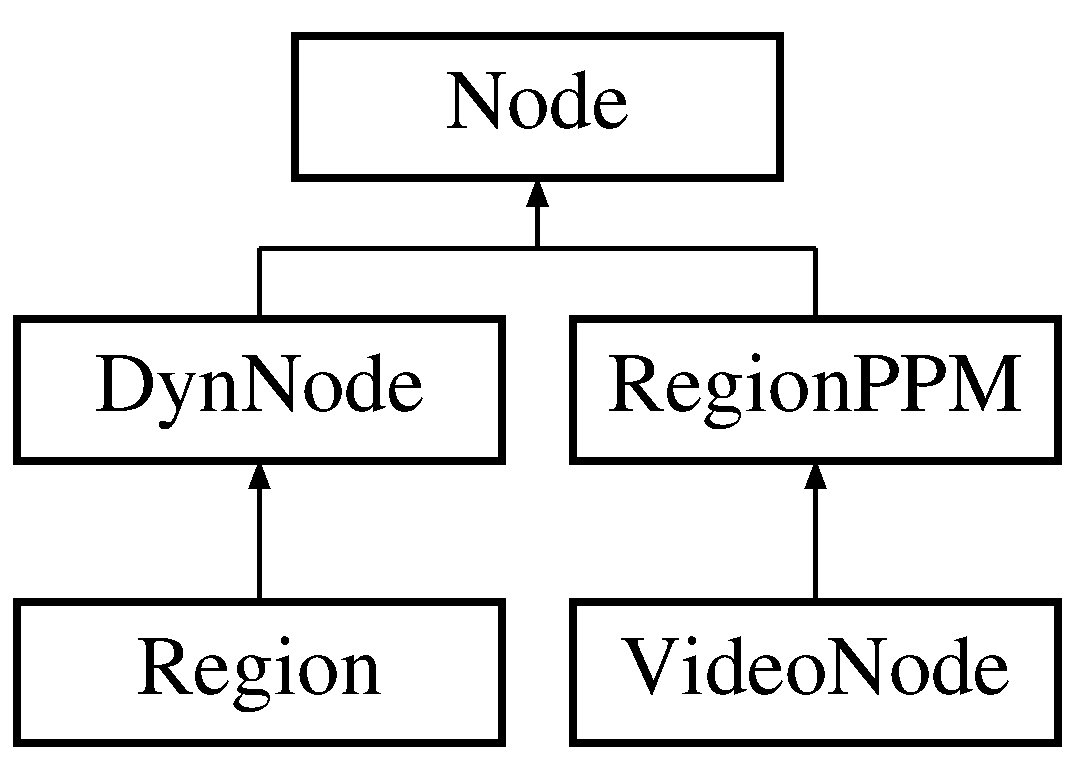
\includegraphics[height=3cm]{classNode}
\end{center}
\end{figure}
\subsection*{Public Member Functions}
\begin{CompactItemize}
\item 
int {\bf getColor} () const
\item 
void {\bf setColor} (int \_\-col)
\item 
{\bf Node} ()
\item 
void {\bf setNodeNumVar} (int \_\-n)
\item 
void {\bf setNodeId} (string \_\-s)
\item 
void {\bf setBelief} ({\bf Belief} $\ast$b)
\item 
{\bf Node} (string s, int {\bf numVar}, {\bf Belief} $\ast$bp=0, int \_\-type=-1)
\item 
int {\bf getNodeNumVar} () const
\item 
string {\bf getNodeId} () const
\item 
{\bf Belief} $\ast$ {\bf getBeliefPtr} ()
\item 
{\bf $\sim$Node} ()
\end{CompactItemize}
\subsection*{Private Attributes}
\begin{CompactItemize}
\item 
int {\bf numVar}
\begin{CompactList}\small\item\em the number of variables at this node \item\end{CompactList}\item 
string {\bf id}
\begin{CompactList}\small\item\em the unique string identifier for this node \item\end{CompactList}\item 
{\bf Belief} $\ast$ {\bf bPtr}
\begin{CompactList}\small\item\em set of beliefs about current state \item\end{CompactList}\item 
{\bf NodeType} {\bf type}
\begin{CompactList}\small\item\em the type of node \item\end{CompactList}\item 
int {\bf color}
\begin{CompactList}\small\item\em used in graph algorithms \item\end{CompactList}\end{CompactItemize}
\subsection*{Friends}
\begin{CompactItemize}
\item 
ostream \& {\bf operator$<$$<$} (ostream \&os, {\bf Node} \&n)
\end{CompactItemize}


\subsection{Detailed Description}
The node class has the following convention regarding naming of the nodes Variable nodes are named as VXXXX ( where XXXX represent numeric code) for example, V012 Factor nodes are named as F\_\-VXXX\_\-VXX ( F representing its a factor ) and VXXX represent the 



\subsection{Constructor \& Destructor Documentation}
\index{Node@{Node}!Node@{Node}}
\index{Node@{Node}!Node@{Node}}
\subsubsection{\setlength{\rightskip}{0pt plus 5cm}Node::Node ()\hspace{0.3cm}{\tt  [inline]}}\label{classNode_74f89688a500bb12a891b0c521284ae1}


\index{Node@{Node}!Node@{Node}}
\index{Node@{Node}!Node@{Node}}
\subsubsection{\setlength{\rightskip}{0pt plus 5cm}Node::Node (string {\em s}, int {\em numVar}, {\bf Belief} $\ast$ {\em bp} = {\tt 0}, int {\em \_\-type} = {\tt -1})}\label{classNode_4ad7f425f80a8769a08aa91f2aa4a542}


\index{Node@{Node}!~Node@{$\sim$Node}}
\index{~Node@{$\sim$Node}!Node@{Node}}
\subsubsection{\setlength{\rightskip}{0pt plus 5cm}Node::$\sim$Node ()\hspace{0.3cm}{\tt  [inline]}}\label{classNode_261e6a1e75de946e7feacb3007165435}




\subsection{Member Function Documentation}
\index{Node@{Node}!getColor@{getColor}}
\index{getColor@{getColor}!Node@{Node}}
\subsubsection{\setlength{\rightskip}{0pt plus 5cm}int Node::getColor () const\hspace{0.3cm}{\tt  [inline]}}\label{classNode_1abe470a6d6918e996c11392cc9c0c20}


\index{Node@{Node}!setColor@{setColor}}
\index{setColor@{setColor}!Node@{Node}}
\subsubsection{\setlength{\rightskip}{0pt plus 5cm}void Node::setColor (int {\em \_\-col})\hspace{0.3cm}{\tt  [inline]}}\label{classNode_85dad9bdc7f7f9564fe432099567b2a6}


\index{Node@{Node}!setNodeNumVar@{setNodeNumVar}}
\index{setNodeNumVar@{setNodeNumVar}!Node@{Node}}
\subsubsection{\setlength{\rightskip}{0pt plus 5cm}void Node::setNodeNumVar (int {\em \_\-n})\hspace{0.3cm}{\tt  [inline]}}\label{classNode_e5c45d621acfbee49dd0b70d10ca3f87}


\index{Node@{Node}!setNodeId@{setNodeId}}
\index{setNodeId@{setNodeId}!Node@{Node}}
\subsubsection{\setlength{\rightskip}{0pt plus 5cm}void Node::setNodeId (string {\em \_\-s})\hspace{0.3cm}{\tt  [inline]}}\label{classNode_9352e0f15cc3ddae82082a59be82d5c2}


\index{Node@{Node}!setBelief@{setBelief}}
\index{setBelief@{setBelief}!Node@{Node}}
\subsubsection{\setlength{\rightskip}{0pt plus 5cm}void Node::setBelief ({\bf Belief} $\ast$ {\em b})\hspace{0.3cm}{\tt  [inline]}}\label{classNode_04293dd9093d19f40f71b2dd67472a59}


\index{Node@{Node}!getNodeNumVar@{getNodeNumVar}}
\index{getNodeNumVar@{getNodeNumVar}!Node@{Node}}
\subsubsection{\setlength{\rightskip}{0pt plus 5cm}int Node::getNodeNumVar () const\hspace{0.3cm}{\tt  [inline]}}\label{classNode_8502fcc64beead4af76420747a22c8ed}


\index{Node@{Node}!getNodeId@{getNodeId}}
\index{getNodeId@{getNodeId}!Node@{Node}}
\subsubsection{\setlength{\rightskip}{0pt plus 5cm}string Node::getNodeId () const\hspace{0.3cm}{\tt  [inline]}}\label{classNode_980889cfdd8c000e8b17f3b968306d58}


\index{Node@{Node}!getBeliefPtr@{getBeliefPtr}}
\index{getBeliefPtr@{getBeliefPtr}!Node@{Node}}
\subsubsection{\setlength{\rightskip}{0pt plus 5cm}{\bf Belief}$\ast$ Node::getBeliefPtr ()\hspace{0.3cm}{\tt  [inline]}}\label{classNode_f7a5e8b045a32c6468ca6d4f3a9233c7}




\subsection{Friends And Related Function Documentation}
\index{Node@{Node}!operator<<@{operator$<$$<$}}
\index{operator<<@{operator$<$$<$}!Node@{Node}}
\subsubsection{\setlength{\rightskip}{0pt plus 5cm}ostream\& operator$<$$<$ (ostream \& {\em os}, {\bf Node} \& {\em n})\hspace{0.3cm}{\tt  [friend]}}\label{classNode_c32ccdb39e5e9cd9f0b919638e049adc}




\subsection{Member Data Documentation}
\index{Node@{Node}!numVar@{numVar}}
\index{numVar@{numVar}!Node@{Node}}
\subsubsection{\setlength{\rightskip}{0pt plus 5cm}int {\bf Node::numVar}\hspace{0.3cm}{\tt  [private]}}\label{classNode_109775531a437cf6f1fa6aa040c8623c}


the number of variables at this node 

\index{Node@{Node}!id@{id}}
\index{id@{id}!Node@{Node}}
\subsubsection{\setlength{\rightskip}{0pt plus 5cm}string {\bf Node::id}\hspace{0.3cm}{\tt  [private]}}\label{classNode_0ac7414e34292f7dfd7f532a69691ca3}


the unique string identifier for this node 

\index{Node@{Node}!bPtr@{bPtr}}
\index{bPtr@{bPtr}!Node@{Node}}
\subsubsection{\setlength{\rightskip}{0pt plus 5cm}{\bf Belief}$\ast$ {\bf Node::bPtr}\hspace{0.3cm}{\tt  [private]}}\label{classNode_fda100bd5a828728ebedff2251861bdf}


set of beliefs about current state 

\index{Node@{Node}!type@{type}}
\index{type@{type}!Node@{Node}}
\subsubsection{\setlength{\rightskip}{0pt plus 5cm}{\bf NodeType} {\bf Node::type}\hspace{0.3cm}{\tt  [private]}}\label{classNode_a791b7bd8347f36b91a1679703a21f91}


the type of node 

\index{Node@{Node}!color@{color}}
\index{color@{color}!Node@{Node}}
\subsubsection{\setlength{\rightskip}{0pt plus 5cm}int {\bf Node::color}\hspace{0.3cm}{\tt  [private]}}\label{classNode_3e6768b832475e9cdaa24be52382115d}


used in graph algorithms 



The documentation for this class was generated from the following files:\begin{CompactItemize}
\item 
inc/{\bf node.h}\item 
src/{\bf node.cpp}\end{CompactItemize}

\section{NodeCmp Struct Reference}
\label{structNodeCmp}\index{NodeCmp@{NodeCmp}}
{\tt \#include $<$node.h$>$}

\subsection*{Public Member Functions}
\begin{CompactItemize}
\item 
bool {\bf operator()} (const {\bf NodePtr} \&n1, const {\bf NodePtr} \&n2) const
\end{CompactItemize}


\subsection{Member Function Documentation}
\index{NodeCmp@{NodeCmp}!operator()@{operator()}}
\index{operator()@{operator()}!NodeCmp@{NodeCmp}}
\subsubsection{\setlength{\rightskip}{0pt plus 5cm}bool NodeCmp::operator() (const {\bf NodePtr} \& {\em n1}, const {\bf NodePtr} \& {\em n2}) const\hspace{0.3cm}{\tt  [inline]}}\label{structNodeCmp_359d377be009f27e3c16464820045ee1}




The documentation for this struct was generated from the following file:\begin{CompactItemize}
\item 
inc/{\bf node.h}\end{CompactItemize}

\section{PottsCB Class Reference}
\label{classPottsCB}\index{PottsCB@{PottsCB}}
{\tt \#include $<$PottsCB.h$>$}

Inheritance diagram for PottsCB::\begin{figure}[H]
\begin{center}
\leavevmode
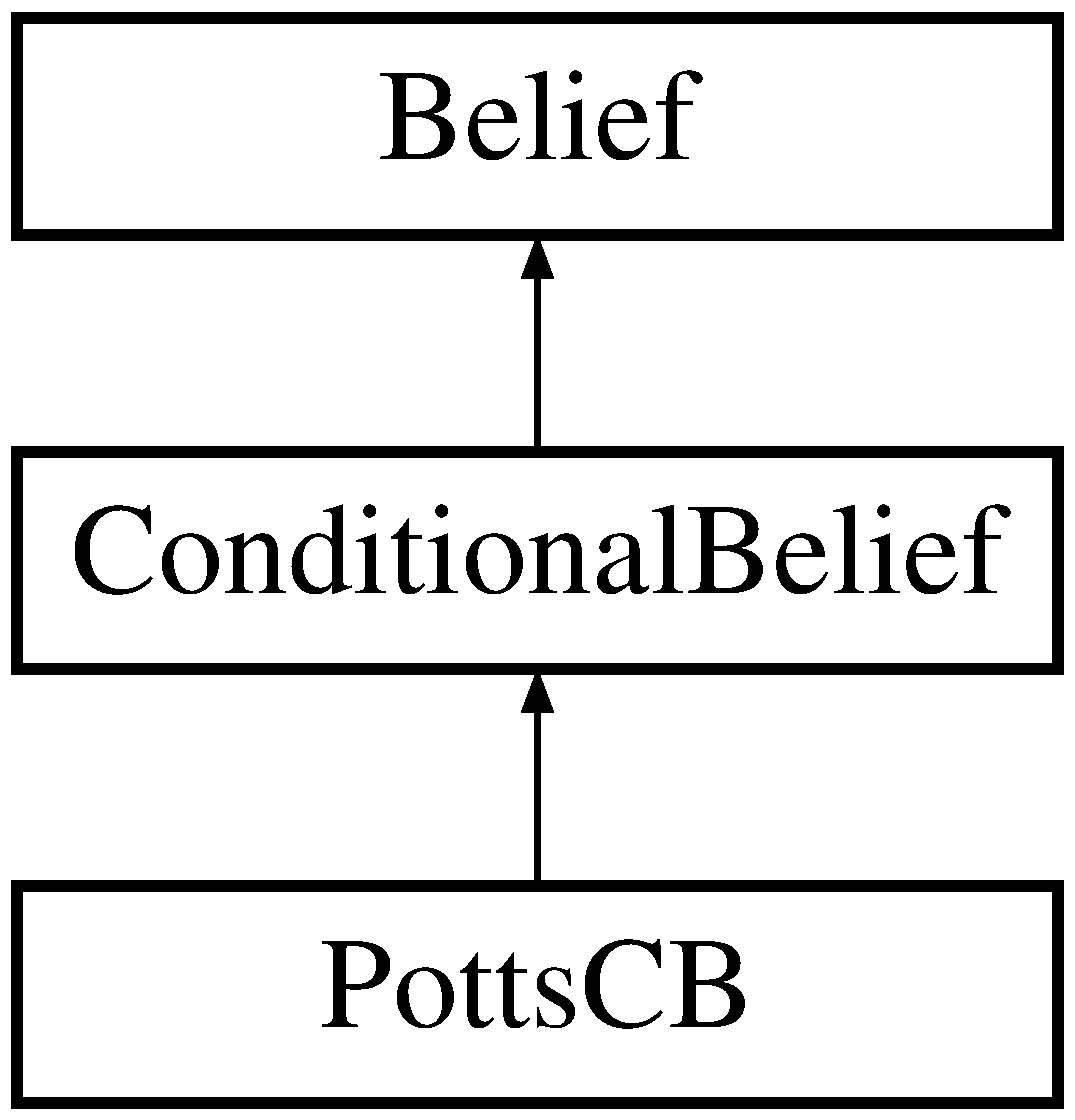
\includegraphics[height=3cm]{classPottsCB}
\end{center}
\end{figure}
\subsection*{Public Member Functions}
\begin{CompactItemize}
\item 
{\bf PottsCB} ({\bf PottsGraphPPM} $\ast$\_\-graph, {\bf VideoNode} $\ast$\_\-node)
\item 
{\bf LD} {\bf getPr} ({\bf StatePtr} s1, {\bf StatePtr} s2)
\begin{CompactList}\small\item\em returns the probability p(sN $|$ sC) or BELIEF\_\-NOT\_\-FOUND \item\end{CompactList}\end{CompactItemize}
\subsection*{Static Public Member Functions}
\begin{CompactItemize}
\item 
static void {\bf setTheta} ({\bf LD} \_\-theta)
\item 
static void {\bf setDt} ({\bf LD} \_\-dt)
\item 
static {\bf LD} {\bf getTheta} ()
\item 
static {\bf LD} {\bf getDt} ()
\end{CompactItemize}
\subsection*{Private Attributes}
\begin{CompactItemize}
\item 
{\bf ConditionalBelief} $\ast$ {\bf cglobal}
\item 
{\bf VideoNode} $\ast$ {\bf node}
\item 
{\bf PottsGraphPPM} $\ast$ {\bf graph}
\end{CompactItemize}
\subsection*{Static Private Attributes}
\begin{CompactItemize}
\item 
static {\bf LD} {\bf theta} = 0.5
\item 
static {\bf LD} {\bf dt} = 1.0
\end{CompactItemize}


\subsection{Constructor \& Destructor Documentation}
\index{PottsCB@{PottsCB}!PottsCB@{PottsCB}}
\index{PottsCB@{PottsCB}!PottsCB@{PottsCB}}
\subsubsection{\setlength{\rightskip}{0pt plus 5cm}PottsCB::PottsCB ({\bf PottsGraphPPM} $\ast$ {\em \_\-graph}, {\bf VideoNode} $\ast$ {\em \_\-node})\hspace{0.3cm}{\tt  [inline]}}\label{classPottsCB_0fff4e248302331be0b38564235d83b1}




\subsection{Member Function Documentation}
\index{PottsCB@{PottsCB}!setTheta@{setTheta}}
\index{setTheta@{setTheta}!PottsCB@{PottsCB}}
\subsubsection{\setlength{\rightskip}{0pt plus 5cm}static void PottsCB::setTheta ({\bf LD} {\em \_\-theta})\hspace{0.3cm}{\tt  [inline, static]}}\label{classPottsCB_b482436f068a16eb7f7d0de838b28815}


\index{PottsCB@{PottsCB}!setDt@{setDt}}
\index{setDt@{setDt}!PottsCB@{PottsCB}}
\subsubsection{\setlength{\rightskip}{0pt plus 5cm}static void PottsCB::setDt ({\bf LD} {\em \_\-dt})\hspace{0.3cm}{\tt  [inline, static]}}\label{classPottsCB_8bec85a1bf2c7f1ba4de6dc944bae647}


\index{PottsCB@{PottsCB}!getTheta@{getTheta}}
\index{getTheta@{getTheta}!PottsCB@{PottsCB}}
\subsubsection{\setlength{\rightskip}{0pt plus 5cm}static {\bf LD} PottsCB::getTheta ()\hspace{0.3cm}{\tt  [inline, static]}}\label{classPottsCB_2d41992ff2e6516c344e501550501cd6}


\index{PottsCB@{PottsCB}!getDt@{getDt}}
\index{getDt@{getDt}!PottsCB@{PottsCB}}
\subsubsection{\setlength{\rightskip}{0pt plus 5cm}static {\bf LD} PottsCB::getDt ()\hspace{0.3cm}{\tt  [inline, static]}}\label{classPottsCB_2d3de42946f700c9ea430a8c37cec9a1}


\index{PottsCB@{PottsCB}!getPr@{getPr}}
\index{getPr@{getPr}!PottsCB@{PottsCB}}
\subsubsection{\setlength{\rightskip}{0pt plus 5cm}{\bf LD} PottsCB::getPr ({\bf StatePtr} {\em sC}, {\bf StatePtr} {\em sN})}\label{classPottsCB_cac254c4f74d94caa1ba23343e01b96b}


returns the probability p(sN $|$ sC) or BELIEF\_\-NOT\_\-FOUND 



Reimplemented from {\bf ConditionalBelief} \doxyref{}{p.}{classConditionalBelief_66ced9bc695d3503e06a02ca95207a21}.

\subsection{Member Data Documentation}
\index{PottsCB@{PottsCB}!cglobal@{cglobal}}
\index{cglobal@{cglobal}!PottsCB@{PottsCB}}
\subsubsection{\setlength{\rightskip}{0pt plus 5cm}{\bf ConditionalBelief}$\ast$ {\bf PottsCB::cglobal}\hspace{0.3cm}{\tt  [private]}}\label{classPottsCB_8a715f9dcc4f2e3272bfb0ec39723a26}


\index{PottsCB@{PottsCB}!node@{node}}
\index{node@{node}!PottsCB@{PottsCB}}
\subsubsection{\setlength{\rightskip}{0pt plus 5cm}{\bf VideoNode}$\ast$ {\bf PottsCB::node}\hspace{0.3cm}{\tt  [private]}}\label{classPottsCB_8bda4193bb8a73ce8426f47b26e6cc3b}


\index{PottsCB@{PottsCB}!graph@{graph}}
\index{graph@{graph}!PottsCB@{PottsCB}}
\subsubsection{\setlength{\rightskip}{0pt plus 5cm}{\bf PottsGraphPPM}$\ast$ {\bf PottsCB::graph}\hspace{0.3cm}{\tt  [private]}}\label{classPottsCB_24db84e3bc0272263622910fef0b5187}


\index{PottsCB@{PottsCB}!theta@{theta}}
\index{theta@{theta}!PottsCB@{PottsCB}}
\subsubsection{\setlength{\rightskip}{0pt plus 5cm}{\bf LD} {\bf PottsCB::theta} = 0.5\hspace{0.3cm}{\tt  [static, private]}}\label{classPottsCB_79d24daa20329a81ab26e16a3ae99a0e}


\index{PottsCB@{PottsCB}!dt@{dt}}
\index{dt@{dt}!PottsCB@{PottsCB}}
\subsubsection{\setlength{\rightskip}{0pt plus 5cm}{\bf LD} {\bf PottsCB::dt} = 1.0\hspace{0.3cm}{\tt  [static, private]}}\label{classPottsCB_4c46b6eae4fe985f7e8f8d0ad0716582}




The documentation for this class was generated from the following files:\begin{CompactItemize}
\item 
inc/{\bf PottsCB.h}\item 
src/{\bf PottsCB.cpp}\end{CompactItemize}

\section{PottsGraphPPM Class Reference}
\label{classPottsGraphPPM}\index{PottsGraphPPM@{PottsGraphPPM}}
{\tt \#include $<$PottsGraph.h$>$}

Inheritance diagram for PottsGraphPPM::\begin{figure}[H]
\begin{center}
\leavevmode
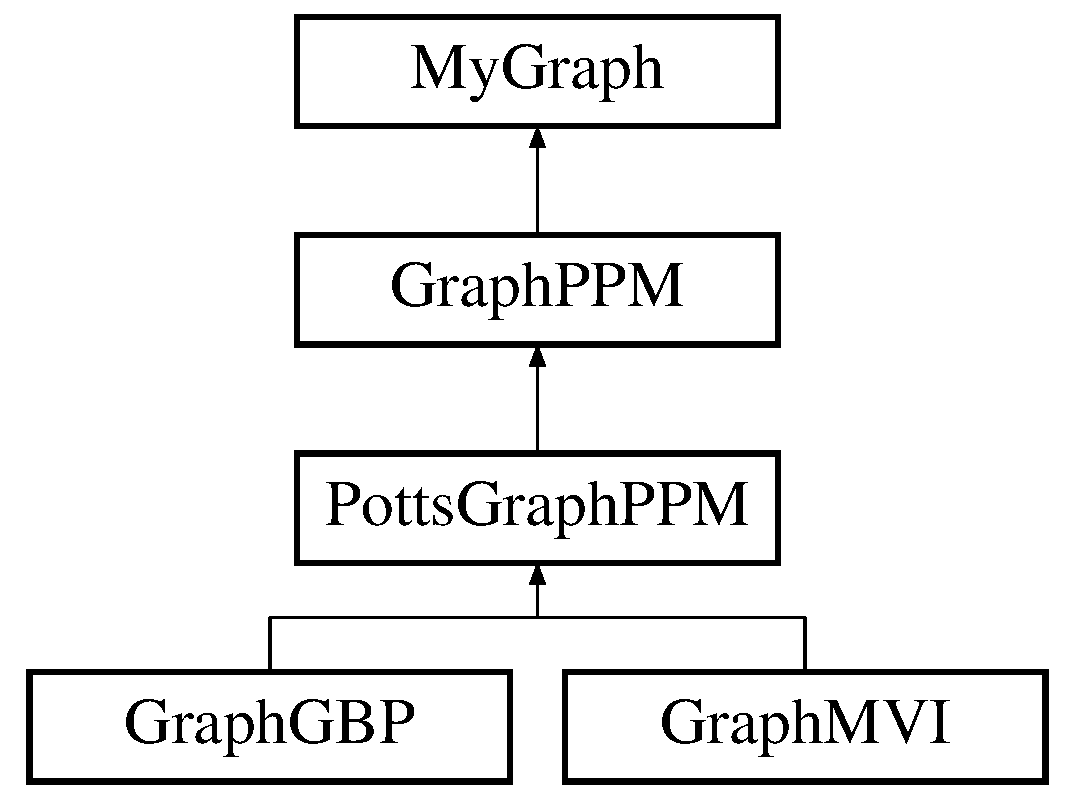
\includegraphics[height=4cm]{classPottsGraphPPM}
\end{center}
\end{figure}
\subsection*{Public Member Functions}
\begin{CompactItemize}
\item 
{\bf PottsGraphPPM} ({\bf PottsModel} $\ast$\_\-M, int \_\-rx, int \_\-ry, int \_\-cx, int \_\-cy)
\item 
void {\bf genSubRegions} ()
\item 
{\bf VideoNode} $\ast$ {\bf addNode} ({\bf VideoNode} $\ast$)
\item 
vector$<$ {\bf INT} $>$ {\bf getIthStVec} (int idx, int N)
\item 
void {\bf initOrigP} ({\bf VideoNode} $\ast$vn, bool rndm=true)
\item 
void {\bf PPM\_\-step2} ({\bf LD} theta, {\bf LD} {\bf delta\_\-t})
\begin{CompactList}\small\item\em Initializes the single belief and conditional belief values;. \item\end{CompactList}\item 
{\bf LD} {\bf getStatePr} ({\bf VideoNode} $\ast$vn, {\bf StatePtr} sp)
\item 
{\bf LD} {\bf get\_\-p\_\-hat} ({\bf VideoNode} $\ast$vn, {\bf StatePtr} si, {\bf StatePtr} so, {\bf LD} theta, {\bf LD} dt)
\item 
void {\bf initCondP} ({\bf VideoNode} $\ast$vn, {\bf LD} theta, {\bf LD} dt)
\item 
{\bf StatePtr} {\bf getChildStatePtr} ({\bf NodePtr} vp, {\bf NodePtr} vc, {\bf StatePtr} parState)
\item 
void {\bf PPM\_\-algo} ({\bf LD} theta, {\bf LD} dt)
\item 
void {\bf PPM\_\-algo2} ({\bf LD} theta, {\bf LD} dt)
\item 
{\bf LD} {\bf getHR} ()
\item 
void {\bf initFG} ()
\item 
{\bf LD} {\bf getVarMargPr} ({\bf VideoNode} $\ast$, int x, int y, int val)
\item 
{\bf LD} {\bf updateTime} ({\bf LD} dt)
\item 
bool {\bf stoppingCriterion} (int iter, {\bf LD} PD\_\-thres=0.05, {\bf LD} blf\_\-thres=0.05, int iter\_\-thres=4)
\item 
vector$<$ vector$<$ {\bf INT} $>$ $>$ {\bf greedyDecision} ()
\item 
void {\bf singleIter} ({\bf LD} theta\_\-ppm, {\bf LD} dt\_\-ppm)
\item 
void {\bf initAllNodesOrigP} (bool rndm)
\item 
bool {\bf isValid} (int x, int y)
\item 
void {\bf genBETHE} ()
\item 
vector$<$ {\bf LD} $>$ {\bf getNormGraphBlfs} ()
\item 
{\bf LD} {\bf getGraphStBlf} (int i)
\item 
void {\bf writeModelFile} (FILE $\ast$modelFile)
\begin{CompactList}\small\item\em generates the ampl model file \item\end{CompactList}\item 
void {\bf getAMPL} (string modelFileName, string dataFileName, string amplFileName)
\begin{CompactList}\small\item\em generates the ampl files for simulating a single ppm iteration \item\end{CompactList}\end{CompactItemize}
\subsection*{Public Attributes}
\begin{CompactItemize}
\item 
{\bf PottsModel} $\ast$ {\bf model}
\item 
int {\bf rx}
\item 
int {\bf ry}
\item 
int {\bf cx}
\item 
int {\bf cy}
\item 
{\bf FactorGraph} $\ast$ {\bf fg}
\item 
{\bf LD} {\bf currTime}
\item 
{\bf LD} {\bf currDt}
\end{CompactItemize}


\subsection{Constructor \& Destructor Documentation}
\index{PottsGraphPPM@{PottsGraphPPM}!PottsGraphPPM@{PottsGraphPPM}}
\index{PottsGraphPPM@{PottsGraphPPM}!PottsGraphPPM@{PottsGraphPPM}}
\subsubsection{\setlength{\rightskip}{0pt plus 5cm}PottsGraphPPM::PottsGraphPPM ({\bf PottsModel} $\ast$ {\em \_\-M}, int {\em \_\-rx}, int {\em \_\-ry}, int {\em \_\-cx}, int {\em \_\-cy})\hspace{0.3cm}{\tt  [inline]}}\label{classPottsGraphPPM_f8be4c8855c9ead438b42f9712c26918}




\subsection{Member Function Documentation}
\index{PottsGraphPPM@{PottsGraphPPM}!genSubRegions@{genSubRegions}}
\index{genSubRegions@{genSubRegions}!PottsGraphPPM@{PottsGraphPPM}}
\subsubsection{\setlength{\rightskip}{0pt plus 5cm}void PottsGraphPPM::genSubRegions ()}\label{classPottsGraphPPM_dda218702c5f95f527a1f0a723a2fcc8}


Modified genSubRegions - uses cluster counting approach \index{PottsGraphPPM@{PottsGraphPPM}!addNode@{addNode}}
\index{addNode@{addNode}!PottsGraphPPM@{PottsGraphPPM}}
\subsubsection{\setlength{\rightskip}{0pt plus 5cm}{\bf VideoNode} $\ast$ PottsGraphPPM::addNode ({\bf VideoNode} $\ast$)}\label{classPottsGraphPPM_46e22df9510aabf6dfd41c41d051569f}


\index{PottsGraphPPM@{PottsGraphPPM}!getIthStVec@{getIthStVec}}
\index{getIthStVec@{getIthStVec}!PottsGraphPPM@{PottsGraphPPM}}
\subsubsection{\setlength{\rightskip}{0pt plus 5cm}vector$<$ {\bf INT} $>$ PottsGraphPPM::getIthStVec (int {\em idx}, int {\em N})}\label{classPottsGraphPPM_fe5c2e29ab0e74699bb76c357bc8322b}


\index{PottsGraphPPM@{PottsGraphPPM}!initOrigP@{initOrigP}}
\index{initOrigP@{initOrigP}!PottsGraphPPM@{PottsGraphPPM}}
\subsubsection{\setlength{\rightskip}{0pt plus 5cm}void PottsGraphPPM::initOrigP ({\bf VideoNode} $\ast$ {\em vn}, bool {\em rndm} = {\tt true})}\label{classPottsGraphPPM_5479d7486144080079066f3e234c43ef}


\index{PottsGraphPPM@{PottsGraphPPM}!PPM_step2@{PPM\_\-step2}}
\index{PPM_step2@{PPM\_\-step2}!PottsGraphPPM@{PottsGraphPPM}}
\subsubsection{\setlength{\rightskip}{0pt plus 5cm}void PottsGraphPPM::PPM\_\-step2 ({\bf LD} {\em theta}, {\bf LD} {\em delta\_\-t})}\label{classPottsGraphPPM_f1f826adcd1466bf659b9dc34f08b7cf}


Initializes the single belief and conditional belief values;. 

\index{PottsGraphPPM@{PottsGraphPPM}!getStatePr@{getStatePr}}
\index{getStatePr@{getStatePr}!PottsGraphPPM@{PottsGraphPPM}}
\subsubsection{\setlength{\rightskip}{0pt plus 5cm}{\bf LD} PottsGraphPPM::getStatePr ({\bf VideoNode} $\ast$ {\em vn}, {\bf StatePtr} {\em sp})}\label{classPottsGraphPPM_03ceec5a5ddb5b33d1b1acb2926265b9}




Reimplemented in {\bf GraphMVI} \doxyref{}{p.}{classGraphMVI_8751683935447989fb988382955dbc02}.\index{PottsGraphPPM@{PottsGraphPPM}!get_p_hat@{get\_\-p\_\-hat}}
\index{get_p_hat@{get\_\-p\_\-hat}!PottsGraphPPM@{PottsGraphPPM}}
\subsubsection{\setlength{\rightskip}{0pt plus 5cm}{\bf LD} PottsGraphPPM::get\_\-p\_\-hat ({\bf VideoNode} $\ast$ {\em vn}, {\bf StatePtr} {\em si}, {\bf StatePtr} {\em so}, {\bf LD} {\em theta}, {\bf LD} {\em dt})}\label{classPottsGraphPPM_b735fb1d57301afad4cdc14ffd5a6252}




Reimplemented in {\bf GraphMVI} \doxyref{}{p.}{classGraphMVI_f2a1f00572448ffe7568d0c927bfcc51}.\index{PottsGraphPPM@{PottsGraphPPM}!initCondP@{initCondP}}
\index{initCondP@{initCondP}!PottsGraphPPM@{PottsGraphPPM}}
\subsubsection{\setlength{\rightskip}{0pt plus 5cm}void PottsGraphPPM::initCondP ({\bf VideoNode} $\ast$ {\em vn}, {\bf LD} {\em theta}, {\bf LD} {\em dt})}\label{classPottsGraphPPM_276673597baefb6b317b96efe23815fa}




Reimplemented in {\bf GraphMVI} \doxyref{}{p.}{classGraphMVI_5137366e48b2928a20236e8851ae5e4b}.\index{PottsGraphPPM@{PottsGraphPPM}!getChildStatePtr@{getChildStatePtr}}
\index{getChildStatePtr@{getChildStatePtr}!PottsGraphPPM@{PottsGraphPPM}}
\subsubsection{\setlength{\rightskip}{0pt plus 5cm}{\bf StatePtr} PottsGraphPPM::getChildStatePtr ({\bf NodePtr} {\em vp}, {\bf NodePtr} {\em vc}, {\bf StatePtr} {\em parState})\hspace{0.3cm}{\tt  [virtual]}}\label{classPottsGraphPPM_7422e923b897b8799ab7de73e3f10088}




Implements {\bf GraphPPM} \doxyref{}{p.}{classGraphPPM_b245aae058d0b252df985651c8fcc2eb}.\index{PottsGraphPPM@{PottsGraphPPM}!PPM_algo@{PPM\_\-algo}}
\index{PPM_algo@{PPM\_\-algo}!PottsGraphPPM@{PottsGraphPPM}}
\subsubsection{\setlength{\rightskip}{0pt plus 5cm}void PottsGraphPPM::PPM\_\-algo ({\bf LD} {\em theta}, {\bf LD} {\em dt})}\label{classPottsGraphPPM_e644a21cf2bd710deec76248b4edfec0}


\index{PottsGraphPPM@{PottsGraphPPM}!PPM_algo2@{PPM\_\-algo2}}
\index{PPM_algo2@{PPM\_\-algo2}!PottsGraphPPM@{PottsGraphPPM}}
\subsubsection{\setlength{\rightskip}{0pt plus 5cm}void PottsGraphPPM::PPM\_\-algo2 ({\bf LD} {\em theta}, {\bf LD} {\em dt})}\label{classPottsGraphPPM_4fb4b1ae6c5b1eeb493b16d7ed50de54}


\index{PottsGraphPPM@{PottsGraphPPM}!getHR@{getHR}}
\index{getHR@{getHR}!PottsGraphPPM@{PottsGraphPPM}}
\subsubsection{\setlength{\rightskip}{0pt plus 5cm}{\bf LD} PottsGraphPPM::getHR ()}\label{classPottsGraphPPM_82288c12c224d84cf5e4fb52a0397662}


\index{PottsGraphPPM@{PottsGraphPPM}!initFG@{initFG}}
\index{initFG@{initFG}!PottsGraphPPM@{PottsGraphPPM}}
\subsubsection{\setlength{\rightskip}{0pt plus 5cm}void PottsGraphPPM::initFG ()}\label{classPottsGraphPPM_ee7a610393b59ce394d296f4e7a60e90}


\index{PottsGraphPPM@{PottsGraphPPM}!getVarMargPr@{getVarMargPr}}
\index{getVarMargPr@{getVarMargPr}!PottsGraphPPM@{PottsGraphPPM}}
\subsubsection{\setlength{\rightskip}{0pt plus 5cm}{\bf LD} PottsGraphPPM::getVarMargPr ({\bf VideoNode} $\ast$, int {\em x}, int {\em y}, int {\em val})}\label{classPottsGraphPPM_ed04ade9cfbdc8284fad3fa93e402572}


\index{PottsGraphPPM@{PottsGraphPPM}!updateTime@{updateTime}}
\index{updateTime@{updateTime}!PottsGraphPPM@{PottsGraphPPM}}
\subsubsection{\setlength{\rightskip}{0pt plus 5cm}{\bf LD} PottsGraphPPM::updateTime ({\bf LD} {\em dt})}\label{classPottsGraphPPM_9cac6ffa0063ec4e5a3102f93bd2da92}




Reimplemented in {\bf GraphMVI} \doxyref{}{p.}{classGraphMVI_25b13c96f42a85b5ed3d7e6068e1659c}.\index{PottsGraphPPM@{PottsGraphPPM}!stoppingCriterion@{stoppingCriterion}}
\index{stoppingCriterion@{stoppingCriterion}!PottsGraphPPM@{PottsGraphPPM}}
\subsubsection{\setlength{\rightskip}{0pt plus 5cm}bool PottsGraphPPM::stoppingCriterion (int {\em iter}, {\bf LD} {\em PD\_\-thres} = {\tt 0.05}, {\bf LD} {\em blf\_\-thres} = {\tt 0.05}, int {\em iter\_\-thres} = {\tt 4})}\label{classPottsGraphPPM_f9ea81fe41e9aec45ba35af11070cd9a}


\index{PottsGraphPPM@{PottsGraphPPM}!greedyDecision@{greedyDecision}}
\index{greedyDecision@{greedyDecision}!PottsGraphPPM@{PottsGraphPPM}}
\subsubsection{\setlength{\rightskip}{0pt plus 5cm}vector$<$ vector$<$ {\bf INT} $>$ $>$ PottsGraphPPM::greedyDecision ()}\label{classPottsGraphPPM_ca61fb275a93940417ad98020d6f9114}


\index{PottsGraphPPM@{PottsGraphPPM}!singleIter@{singleIter}}
\index{singleIter@{singleIter}!PottsGraphPPM@{PottsGraphPPM}}
\subsubsection{\setlength{\rightskip}{0pt plus 5cm}void PottsGraphPPM::singleIter ({\bf LD} {\em theta\_\-ppm}, {\bf LD} {\em dt\_\-ppm})}\label{classPottsGraphPPM_3da7d2a78fc1d560131719162406b6e0}


\index{PottsGraphPPM@{PottsGraphPPM}!initAllNodesOrigP@{initAllNodesOrigP}}
\index{initAllNodesOrigP@{initAllNodesOrigP}!PottsGraphPPM@{PottsGraphPPM}}
\subsubsection{\setlength{\rightskip}{0pt plus 5cm}void PottsGraphPPM::initAllNodesOrigP (bool {\em rndm})}\label{classPottsGraphPPM_db429e7e4eac1a4d69f641403735cb20}




Reimplemented in {\bf GraphMVI} \doxyref{}{p.}{classGraphMVI_1033e03be9c66b7ff356c7bb0e8fe083}.\index{PottsGraphPPM@{PottsGraphPPM}!isValid@{isValid}}
\index{isValid@{isValid}!PottsGraphPPM@{PottsGraphPPM}}
\subsubsection{\setlength{\rightskip}{0pt plus 5cm}bool PottsGraphPPM::isValid (int {\em x}, int {\em y})}\label{classPottsGraphPPM_9c953796371a26e9284b33b607ddaa3a}


\index{PottsGraphPPM@{PottsGraphPPM}!genBETHE@{genBETHE}}
\index{genBETHE@{genBETHE}!PottsGraphPPM@{PottsGraphPPM}}
\subsubsection{\setlength{\rightskip}{0pt plus 5cm}void PottsGraphPPM::genBETHE ()}\label{classPottsGraphPPM_237da04ddb08a9bd6e6eba6ce8ad37f4}


\index{PottsGraphPPM@{PottsGraphPPM}!getNormGraphBlfs@{getNormGraphBlfs}}
\index{getNormGraphBlfs@{getNormGraphBlfs}!PottsGraphPPM@{PottsGraphPPM}}
\subsubsection{\setlength{\rightskip}{0pt plus 5cm}vector$<$ {\bf LD} $>$ PottsGraphPPM::getNormGraphBlfs ()}\label{classPottsGraphPPM_45b72b847bc40680ee02394242ef129b}


Returns the normalized beliefs as a product of region beliefs with appropriate normalization \index{PottsGraphPPM@{PottsGraphPPM}!getGraphStBlf@{getGraphStBlf}}
\index{getGraphStBlf@{getGraphStBlf}!PottsGraphPPM@{PottsGraphPPM}}
\subsubsection{\setlength{\rightskip}{0pt plus 5cm}{\bf LD} PottsGraphPPM::getGraphStBlf (int {\em i})}\label{classPottsGraphPPM_9f806329c39a15d743dbc2081c505090}


\index{PottsGraphPPM@{PottsGraphPPM}!writeModelFile@{writeModelFile}}
\index{writeModelFile@{writeModelFile}!PottsGraphPPM@{PottsGraphPPM}}
\subsubsection{\setlength{\rightskip}{0pt plus 5cm}void PottsGraphPPM::writeModelFile (FILE $\ast$ {\em modeFile})}\label{classPottsGraphPPM_82a6be96d8bcb0efe1b9efa65ff596ae}


generates the ampl model file 

\begin{itemize}
\item modelFile \end{itemize}
\index{PottsGraphPPM@{PottsGraphPPM}!getAMPL@{getAMPL}}
\index{getAMPL@{getAMPL}!PottsGraphPPM@{PottsGraphPPM}}
\subsubsection{\setlength{\rightskip}{0pt plus 5cm}void PottsGraphPPM::getAMPL (string {\em modelFileName}, string {\em dataFileName}, string {\em commandFileName})}\label{classPottsGraphPPM_788ca1208dd0acc57fffb10861af5c89}


generates the ampl files for simulating a single ppm iteration 

\begin{itemize}
\item modelFileName the AMPL model file generated \item dataFileName the AMPL data file generated \item commandFileName the file containing AMPL execution code \begin{Desc}
\item[Note:]The AMPL code has the following parameters: \par
 params: q, c\_\-alpha(rgn), numVar(rgn), b1\_\-rgn(1..q$^\wedge$n) , p2\_\-rgn(1..q$^\wedge$n) \par
 vars: b2\_\-rgn(1..q$^\wedge$n, 1..q$^\wedge$n) \end{Desc}
\end{itemize}


\subsection{Member Data Documentation}
\index{PottsGraphPPM@{PottsGraphPPM}!model@{model}}
\index{model@{model}!PottsGraphPPM@{PottsGraphPPM}}
\subsubsection{\setlength{\rightskip}{0pt plus 5cm}{\bf PottsModel}$\ast$ {\bf PottsGraphPPM::model}}\label{classPottsGraphPPM_e2575319241eacadb69eb75e18803f22}


\index{PottsGraphPPM@{PottsGraphPPM}!rx@{rx}}
\index{rx@{rx}!PottsGraphPPM@{PottsGraphPPM}}
\subsubsection{\setlength{\rightskip}{0pt plus 5cm}int {\bf PottsGraphPPM::rx}}\label{classPottsGraphPPM_d79c302008f13e7c759e739d578afba2}


\index{PottsGraphPPM@{PottsGraphPPM}!ry@{ry}}
\index{ry@{ry}!PottsGraphPPM@{PottsGraphPPM}}
\subsubsection{\setlength{\rightskip}{0pt plus 5cm}int {\bf PottsGraphPPM::ry}}\label{classPottsGraphPPM_f1e687e6ee33ef5bf2b3e8056b723404}


\index{PottsGraphPPM@{PottsGraphPPM}!cx@{cx}}
\index{cx@{cx}!PottsGraphPPM@{PottsGraphPPM}}
\subsubsection{\setlength{\rightskip}{0pt plus 5cm}int {\bf PottsGraphPPM::cx}}\label{classPottsGraphPPM_4087f2bf0129f3bb68a9eb6469b66560}


\index{PottsGraphPPM@{PottsGraphPPM}!cy@{cy}}
\index{cy@{cy}!PottsGraphPPM@{PottsGraphPPM}}
\subsubsection{\setlength{\rightskip}{0pt plus 5cm}int {\bf PottsGraphPPM::cy}}\label{classPottsGraphPPM_b88eb62241b96af01c31792360fc709b}


\index{PottsGraphPPM@{PottsGraphPPM}!fg@{fg}}
\index{fg@{fg}!PottsGraphPPM@{PottsGraphPPM}}
\subsubsection{\setlength{\rightskip}{0pt plus 5cm}{\bf FactorGraph}$\ast$ {\bf PottsGraphPPM::fg}}\label{classPottsGraphPPM_381af46e5706ce7d18afce26c5fa8e9e}


\index{PottsGraphPPM@{PottsGraphPPM}!currTime@{currTime}}
\index{currTime@{currTime}!PottsGraphPPM@{PottsGraphPPM}}
\subsubsection{\setlength{\rightskip}{0pt plus 5cm}{\bf LD} {\bf PottsGraphPPM::currTime}}\label{classPottsGraphPPM_0b8f10e6fc78d6358eddff02be9ff97a}


\index{PottsGraphPPM@{PottsGraphPPM}!currDt@{currDt}}
\index{currDt@{currDt}!PottsGraphPPM@{PottsGraphPPM}}
\subsubsection{\setlength{\rightskip}{0pt plus 5cm}{\bf LD} {\bf PottsGraphPPM::currDt}}\label{classPottsGraphPPM_29f24f2a7b11476bb017905403c169ce}




The documentation for this class was generated from the following files:\begin{CompactItemize}
\item 
inc/{\bf PottsGraph.h}\item 
src/{\bf PottsGraph.cpp}\end{CompactItemize}

\section{PottsModel Struct Reference}
\label{structPottsModel}\index{PottsModel@{PottsModel}}
{\tt \#include $<$PottsModel.h$>$}

Inheritance diagram for PottsModel::\begin{figure}[H]
\begin{center}
\leavevmode
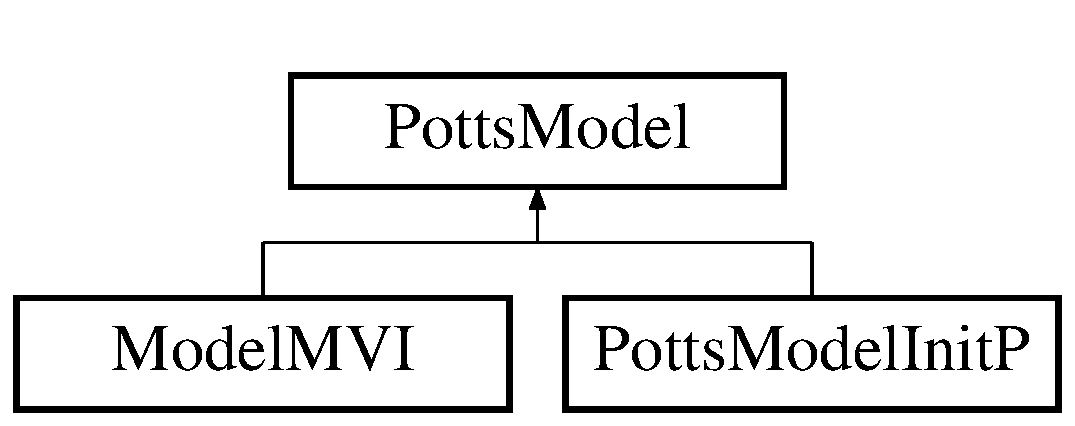
\includegraphics[height=2cm]{structPottsModel}
\end{center}
\end{figure}
\subsection*{Public Member Functions}
\begin{CompactItemize}
\item 
{\bf PottsModel} (int \_\-N1, int \_\-N2, int \_\-Q=2, {\bf LD} \_\-jSigma=0.1, {\bf LD} \_\-hSigma=0.1, int \_\-seed=0)
\item 
void {\bf genNodes} ()
\item 
void {\bf updateBlfPtr} ({\bf BeliefPtr} bNew, int varNum)
\item 
int {\bf GV} (int k)
\item 
bool {\bf isValid} (int r, int c)
\item 
string {\bf getStats} ()
\item 
void {\bf genFactors} ()
\item 
{\bf LD} {\bf getP} (string fid, {\bf StatePtr} sC)
\item 
{\bf LD} {\bf getGlobalP} (int sVal)
\item 
{\bf LD} {\bf getCondP} (int sInit, int sNext, {\bf LD} TD)
\item 
vector$<$ {\bf INT} $>$ {\bf getIthStVec} (int i, int N)
\end{CompactItemize}
\subsection*{Public Attributes}
\begin{CompactItemize}
\item 
int {\bf Q}
\begin{CompactList}\small\item\em the number of possible values each variable can take 1...Q \item\end{CompactList}\item 
{\bf LD} {\bf hSigma}
\begin{CompactList}\small\item\em variance for same node factors \item\end{CompactList}\item 
{\bf LD} {\bf jSigma}
\begin{CompactList}\small\item\em variance for nearest node interactions \item\end{CompactList}\item 
int {\bf N1}
\begin{CompactList}\small\item\em size of the grid \item\end{CompactList}\item 
int {\bf N2}
\item 
int {\bf seed}
\begin{CompactList}\small\item\em the see used for factor generation \item\end{CompactList}\item 
map$<$ string, {\bf BeliefPtr} $>$ {\bf fieldMp}
\begin{CompactList}\small\item\em map containing singular interactions \item\end{CompactList}\item 
gsl\_\-rng $\ast$ {\bf myRNG}
\begin{CompactList}\small\item\em the random number generator \item\end{CompactList}\end{CompactItemize}


\subsection{Constructor \& Destructor Documentation}
\index{PottsModel@{PottsModel}!PottsModel@{PottsModel}}
\index{PottsModel@{PottsModel}!PottsModel@{PottsModel}}
\subsubsection{\setlength{\rightskip}{0pt plus 5cm}PottsModel::PottsModel (int {\em \_\-N1}, int {\em \_\-N2}, int {\em \_\-Q} = {\tt 2}, {\bf LD} {\em \_\-jSigma} = {\tt 0.1}, {\bf LD} {\em \_\-hSigma} = {\tt 0.1}, int {\em \_\-seed} = {\tt 0})\hspace{0.3cm}{\tt  [inline]}}\label{structPottsModel_d500527e03888971fac3845c1ac9a7de}




\subsection{Member Function Documentation}
\index{PottsModel@{PottsModel}!genNodes@{genNodes}}
\index{genNodes@{genNodes}!PottsModel@{PottsModel}}
\subsubsection{\setlength{\rightskip}{0pt plus 5cm}void PottsModel::genNodes ()}\label{structPottsModel_55df917956c272e3ce4a7d9233ecf40b}


\index{PottsModel@{PottsModel}!updateBlfPtr@{updateBlfPtr}}
\index{updateBlfPtr@{updateBlfPtr}!PottsModel@{PottsModel}}
\subsubsection{\setlength{\rightskip}{0pt plus 5cm}void PottsModel::updateBlfPtr ({\bf BeliefPtr} {\em bNew}, int {\em varNum})}\label{structPottsModel_2b2d57c3923af9c22b473f6e9338e969}


\index{PottsModel@{PottsModel}!GV@{GV}}
\index{GV@{GV}!PottsModel@{PottsModel}}
\subsubsection{\setlength{\rightskip}{0pt plus 5cm}int PottsModel::GV (int {\em k})\hspace{0.3cm}{\tt  [inline]}}\label{structPottsModel_5477b77a4b9419c8cdb5a20232a54223}


\index{PottsModel@{PottsModel}!isValid@{isValid}}
\index{isValid@{isValid}!PottsModel@{PottsModel}}
\subsubsection{\setlength{\rightskip}{0pt plus 5cm}bool PottsModel::isValid (int {\em r}, int {\em c})\hspace{0.3cm}{\tt  [inline]}}\label{structPottsModel_96ef879e356b5752fa15507fe816c836}


\index{PottsModel@{PottsModel}!getStats@{getStats}}
\index{getStats@{getStats}!PottsModel@{PottsModel}}
\subsubsection{\setlength{\rightskip}{0pt plus 5cm}string PottsModel::getStats ()}\label{structPottsModel_b47364dbab4dbce1b17ec98c4cbe4984}


\index{PottsModel@{PottsModel}!genFactors@{genFactors}}
\index{genFactors@{genFactors}!PottsModel@{PottsModel}}
\subsubsection{\setlength{\rightskip}{0pt plus 5cm}void PottsModel::genFactors ()}\label{structPottsModel_141ba95ee80197e0d3ae0d8a658b8d07}


\index{PottsModel@{PottsModel}!getP@{getP}}
\index{getP@{getP}!PottsModel@{PottsModel}}
\subsubsection{\setlength{\rightskip}{0pt plus 5cm}{\bf LD} PottsModel::getP (string {\em fid}, {\bf StatePtr} {\em sC})\hspace{0.3cm}{\tt  [inline]}}\label{structPottsModel_ccd5dfd6de009b38b8689be20d04c55f}




Reimplemented in {\bf ModelMVI} \doxyref{}{p.}{classModelMVI_c65577d0b71f762361c063d82e84e478}.\index{PottsModel@{PottsModel}!getGlobalP@{getGlobalP}}
\index{getGlobalP@{getGlobalP}!PottsModel@{PottsModel}}
\subsubsection{\setlength{\rightskip}{0pt plus 5cm}{\bf LD} PottsModel::getGlobalP (int {\em sVal})}\label{structPottsModel_22bc78e573e1eb7d92c3e4a6dd926028}


Returns the proportionality constant - has to be divided by Z(t) to get true probability \index{PottsModel@{PottsModel}!getCondP@{getCondP}}
\index{getCondP@{getCondP}!PottsModel@{PottsModel}}
\subsubsection{\setlength{\rightskip}{0pt plus 5cm}{\bf LD} PottsModel::getCondP (int {\em vInit}, int {\em vNext}, {\bf LD} {\em TD})}\label{structPottsModel_a40d8be472dc2053a045119f3e1a409b}


Returns the P\_\-cond using Kikuchi model \index{PottsModel@{PottsModel}!getIthStVec@{getIthStVec}}
\index{getIthStVec@{getIthStVec}!PottsModel@{PottsModel}}
\subsubsection{\setlength{\rightskip}{0pt plus 5cm}vector$<$ {\bf INT} $>$ PottsModel::getIthStVec (int {\em idx}, int {\em N})}\label{structPottsModel_242908734de9c84adf32148671ff6c85}


Returns the ith state given grid size of N 

\subsection{Member Data Documentation}
\index{PottsModel@{PottsModel}!Q@{Q}}
\index{Q@{Q}!PottsModel@{PottsModel}}
\subsubsection{\setlength{\rightskip}{0pt plus 5cm}int {\bf PottsModel::Q}}\label{structPottsModel_1270472e5682be4105fbbbf44e8173ce}


the number of possible values each variable can take 1...Q 

\index{PottsModel@{PottsModel}!hSigma@{hSigma}}
\index{hSigma@{hSigma}!PottsModel@{PottsModel}}
\subsubsection{\setlength{\rightskip}{0pt plus 5cm}{\bf LD} {\bf PottsModel::hSigma}}\label{structPottsModel_160f94731386c02152b17feba23e0194}


variance for same node factors 

\index{PottsModel@{PottsModel}!jSigma@{jSigma}}
\index{jSigma@{jSigma}!PottsModel@{PottsModel}}
\subsubsection{\setlength{\rightskip}{0pt plus 5cm}{\bf LD} {\bf PottsModel::jSigma}}\label{structPottsModel_c5f84781613bbec83f3dc9a1bae660a3}


variance for nearest node interactions 

\index{PottsModel@{PottsModel}!N1@{N1}}
\index{N1@{N1}!PottsModel@{PottsModel}}
\subsubsection{\setlength{\rightskip}{0pt plus 5cm}int {\bf PottsModel::N1}}\label{structPottsModel_088f56c913125b9858374d4d1aaf744f}


size of the grid 

\index{PottsModel@{PottsModel}!N2@{N2}}
\index{N2@{N2}!PottsModel@{PottsModel}}
\subsubsection{\setlength{\rightskip}{0pt plus 5cm}int {\bf PottsModel::N2}}\label{structPottsModel_dee8cfea7c60a9d460611f5ecbed36c8}


\index{PottsModel@{PottsModel}!seed@{seed}}
\index{seed@{seed}!PottsModel@{PottsModel}}
\subsubsection{\setlength{\rightskip}{0pt plus 5cm}int {\bf PottsModel::seed}}\label{structPottsModel_c7ec124d4d1d82c956b97bf5e592f9ed}


the see used for factor generation 

\index{PottsModel@{PottsModel}!fieldMp@{fieldMp}}
\index{fieldMp@{fieldMp}!PottsModel@{PottsModel}}
\subsubsection{\setlength{\rightskip}{0pt plus 5cm}map$<$string, {\bf BeliefPtr}$>$ {\bf PottsModel::fieldMp}}\label{structPottsModel_610b83e653da7ae2c2c0939037397019}


map containing singular interactions 

\index{PottsModel@{PottsModel}!myRNG@{myRNG}}
\index{myRNG@{myRNG}!PottsModel@{PottsModel}}
\subsubsection{\setlength{\rightskip}{0pt plus 5cm}gsl\_\-rng$\ast$ {\bf PottsModel::myRNG}}\label{structPottsModel_01a7abf9f1d03569a0f2dd639f0e989c}


the random number generator 



The documentation for this struct was generated from the following files:\begin{CompactItemize}
\item 
inc/{\bf PottsModel.h}\item 
src/{\bf PottsModel.cpp}\end{CompactItemize}

\section{PottsModelInitP Struct Reference}
\label{structPottsModelInitP}\index{PottsModelInitP@{PottsModelInitP}}
{\tt \#include $<$PottsModel.h$>$}

Inheritance diagram for PottsModelInitP::\begin{figure}[H]
\begin{center}
\leavevmode
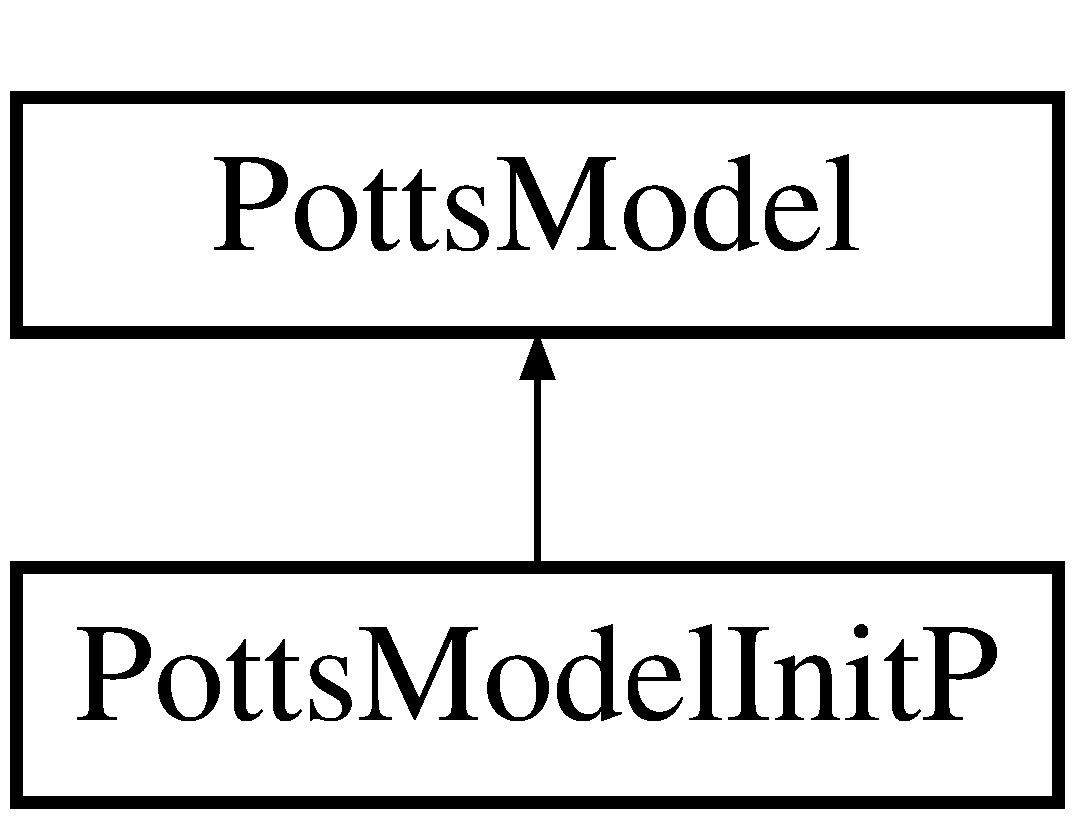
\includegraphics[height=2cm]{structPottsModelInitP}
\end{center}
\end{figure}
\subsection*{Public Member Functions}
\begin{CompactItemize}
\item 
{\bf PottsModelInitP} (int \_\-N1, int \_\-N2, int \_\-Q=2, {\bf LD} \_\-jSigma=0.1, {\bf LD} \_\-hSigma=0.1, int \_\-seed=0)
\item 
void {\bf setInitPseed} (int \_\-s)
\end{CompactItemize}
\subsection*{Public Attributes}
\begin{CompactItemize}
\item 
int {\bf init\_\-p\_\-seed}
\item 
gsl\_\-rng $\ast$ {\bf pRNG}
\end{CompactItemize}


\subsection{Detailed Description}
This class additionally provides the model init b(x\_\-0) which is assumed as factored into singletons - (note) 



\subsection{Constructor \& Destructor Documentation}
\index{PottsModelInitP@{PottsModelInitP}!PottsModelInitP@{PottsModelInitP}}
\index{PottsModelInitP@{PottsModelInitP}!PottsModelInitP@{PottsModelInitP}}
\subsubsection{\setlength{\rightskip}{0pt plus 5cm}PottsModelInitP::PottsModelInitP (int {\em \_\-N1}, int {\em \_\-N2}, int {\em \_\-Q} = {\tt 2}, {\bf LD} {\em \_\-jSigma} = {\tt 0.1}, {\bf LD} {\em \_\-hSigma} = {\tt 0.1}, int {\em \_\-seed} = {\tt 0})\hspace{0.3cm}{\tt  [inline]}}\label{structPottsModelInitP_da6e72d249ce377e013b20535df3461b}




\subsection{Member Function Documentation}
\index{PottsModelInitP@{PottsModelInitP}!setInitPseed@{setInitPseed}}
\index{setInitPseed@{setInitPseed}!PottsModelInitP@{PottsModelInitP}}
\subsubsection{\setlength{\rightskip}{0pt plus 5cm}void PottsModelInitP::setInitPseed (int {\em \_\-s})\hspace{0.3cm}{\tt  [inline]}}\label{structPottsModelInitP_f149dcc6fad10c198c9c41cad879b947}




\subsection{Member Data Documentation}
\index{PottsModelInitP@{PottsModelInitP}!init_p_seed@{init\_\-p\_\-seed}}
\index{init_p_seed@{init\_\-p\_\-seed}!PottsModelInitP@{PottsModelInitP}}
\subsubsection{\setlength{\rightskip}{0pt plus 5cm}int {\bf PottsModelInitP::init\_\-p\_\-seed}}\label{structPottsModelInitP_79d6d88d4ebd7a41e14c98f264049c2e}


\index{PottsModelInitP@{PottsModelInitP}!pRNG@{pRNG}}
\index{pRNG@{pRNG}!PottsModelInitP@{PottsModelInitP}}
\subsubsection{\setlength{\rightskip}{0pt plus 5cm}gsl\_\-rng$\ast$ {\bf PottsModelInitP::pRNG}}\label{structPottsModelInitP_3a7ad4aa95ce6f7fc96b73399aa9b011}




The documentation for this struct was generated from the following file:\begin{CompactItemize}
\item 
inc/{\bf PottsModel.h}\end{CompactItemize}

\section{PRCMP$<$ T, C $>$ Struct Template Reference}
\label{structPRCMP}\index{PRCMP@{PRCMP}}
{\tt \#include $<$main.h$>$}

\subsection*{Public Member Functions}
\begin{CompactItemize}
\item 
bool {\bf operator()} (const pair$<$ T, C $>$ \&p1, const pair$<$ T, C $>$ \&p2) const
\end{CompactItemize}
\subsubsection*{template$<$typename T, typename C$>$ struct PRCMP$<$ T, C $>$}



\subsection{Member Function Documentation}
\index{PRCMP@{PRCMP}!operator()@{operator()}}
\index{operator()@{operator()}!PRCMP@{PRCMP}}
\subsubsection{\setlength{\rightskip}{0pt plus 5cm}template$<$typename T, typename C$>$ bool {\bf PRCMP}$<$ T, C $>$::operator() (const pair$<$ T, C $>$ \& {\em p1}, const pair$<$ T, C $>$ \& {\em p2}) const\hspace{0.3cm}{\tt  [inline]}}\label{structPRCMP_d6ee734553194295afa2732c649f336d}




The documentation for this struct was generated from the following file:\begin{CompactItemize}
\item 
inc/{\bf main.h}\end{CompactItemize}

\section{PRCMP2$<$ T, C $>$ Struct Template Reference}
\label{structPRCMP2}\index{PRCMP2@{PRCMP2}}
{\tt \#include $<$main.h$>$}

\subsection*{Public Member Functions}
\begin{CompactItemize}
\item 
{\bf PRCMP2} (bool \_\-choice=true)
\item 
bool {\bf operator()} (const pair$<$ T, C $>$ \&p1, const pair$<$ T, C $>$ \&p2) const
\end{CompactItemize}
\subsection*{Public Attributes}
\begin{CompactItemize}
\item 
bool {\bf choice}
\end{CompactItemize}
\subsubsection*{template$<$typename T, typename C$>$ struct PRCMP2$<$ T, C $>$}



\subsection{Constructor \& Destructor Documentation}
\index{PRCMP2@{PRCMP2}!PRCMP2@{PRCMP2}}
\index{PRCMP2@{PRCMP2}!PRCMP2@{PRCMP2}}
\subsubsection{\setlength{\rightskip}{0pt plus 5cm}template$<$typename T, typename C$>$ {\bf PRCMP2}$<$ T, C $>$::{\bf PRCMP2} (bool {\em \_\-choice} = {\tt true})\hspace{0.3cm}{\tt  [inline]}}\label{structPRCMP2_d2b672f6725d892ee624caf735d7527b}




\subsection{Member Function Documentation}
\index{PRCMP2@{PRCMP2}!operator()@{operator()}}
\index{operator()@{operator()}!PRCMP2@{PRCMP2}}
\subsubsection{\setlength{\rightskip}{0pt plus 5cm}template$<$typename T, typename C$>$ bool {\bf PRCMP2}$<$ T, C $>$::operator() (const pair$<$ T, C $>$ \& {\em p1}, const pair$<$ T, C $>$ \& {\em p2}) const\hspace{0.3cm}{\tt  [inline]}}\label{structPRCMP2_1e78052b0bdbc6e84380ecccd1240cd1}




\subsection{Member Data Documentation}
\index{PRCMP2@{PRCMP2}!choice@{choice}}
\index{choice@{choice}!PRCMP2@{PRCMP2}}
\subsubsection{\setlength{\rightskip}{0pt plus 5cm}template$<$typename T, typename C$>$ bool {\bf PRCMP2}$<$ T, C $>$::{\bf choice}}\label{structPRCMP2_9032fbaff91306d33791e61d611f6797}




The documentation for this struct was generated from the following file:\begin{CompactItemize}
\item 
inc/{\bf main.h}\end{CompactItemize}

\section{Region Class Reference}
\label{classRegion}\index{Region@{Region}}
{\tt \#include $<$mygraph.h$>$}

Inheritance diagram for Region::\begin{figure}[H]
\begin{center}
\leavevmode
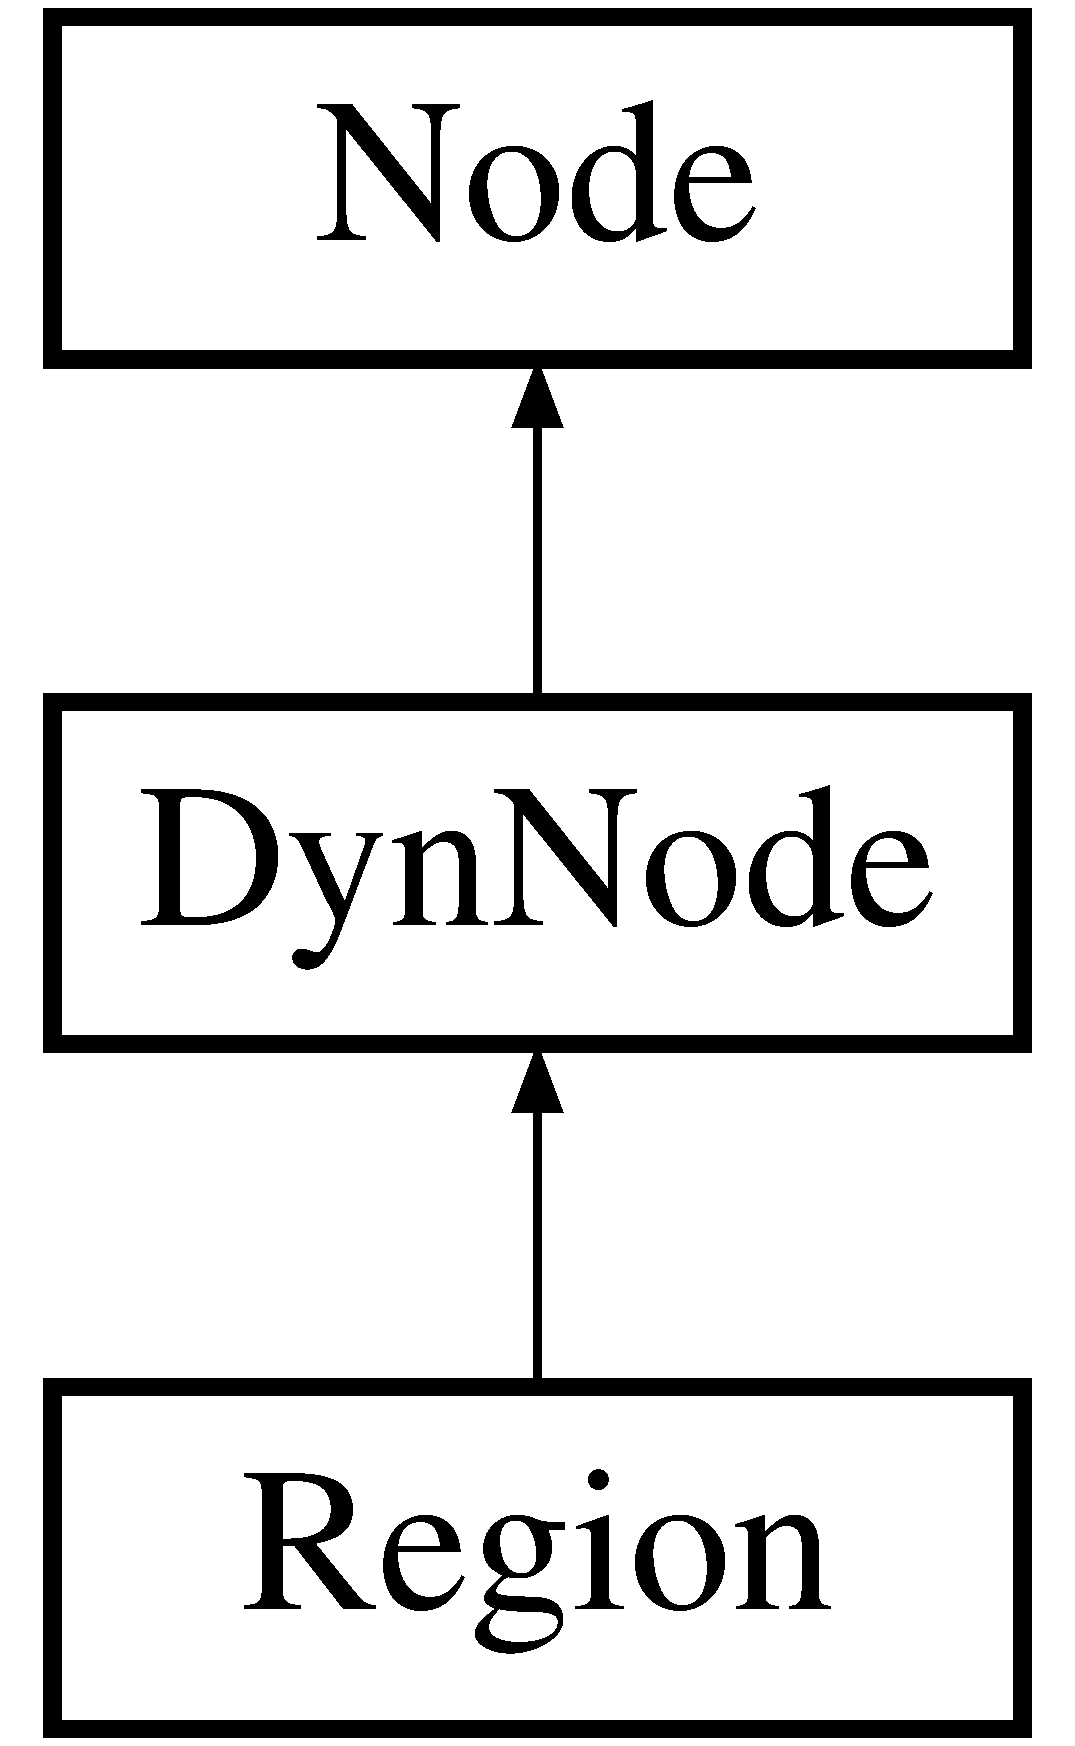
\includegraphics[height=3cm]{classRegion}
\end{center}
\end{figure}
\subsection*{Public Member Functions}
\begin{CompactItemize}
\item 
{\bf Region} ({\bf RegionGraphPtr} \_\-fg, {\bf Cluster} \_\-cl, int \_\-cr, {\bf ConditionalBelief} $\ast$\_\-cb=0)
\item 
{\bf LD} {\bf getStateBlf} (const {\bf StatePtr} sptr) const
\item 
vector$<$ string $>$ {\bf getVarIds} () const
\item 
{\bf LD} {\bf getEntropy} ()
\begin{CompactList}\small\item\em -sum\_\-b b$\ast$log(b) \item\end{CompactList}\item 
{\bf LD} {\bf getEnthalpy} ()
\begin{CompactList}\small\item\em sum\_\-b b$\ast$(-sum\_\-a log f\_\-a) where a is in r \item\end{CompactList}\item 
{\bf LD} {\bf getF} ()
\end{CompactItemize}
\subsection*{Public Attributes}
\begin{CompactItemize}
\item 
int {\bf cr}
\begin{CompactList}\small\item\em counting numbers \item\end{CompactList}\item 
{\bf ConditionalBeliefPtr} {\bf B\_\-t\_\-0}
\begin{CompactList}\small\item\em the K(x0, x\_\-t) factor \item\end{CompactList}\item 
{\bf BeliefPtr} {\bf B\_\-0}
\begin{CompactList}\small\item\em the single ton partition function like function \item\end{CompactList}\item 
{\bf BeliefPtr} {\bf B\_\-t}
\item 
{\bf BeliefPtr} {\bf Z}
\begin{CompactList}\small\item\em the partition function \item\end{CompactList}\end{CompactItemize}
\subsection*{Private Attributes}
\begin{CompactItemize}
\item 
{\bf Cluster} {\bf cl}
\begin{CompactList}\small\item\em the individual factor nodes \item\end{CompactList}\item 
{\bf RegionGraphPtr} {\bf rg}
\item 
{\bf FactorGraphPtr} {\bf fg}
\end{CompactItemize}
\subsection*{Friends}
\begin{CompactItemize}
\item 
ostream \& {\bf operator$<$$<$} (ostream \&os, {\bf Region} \&r)
\end{CompactItemize}


\subsection{Detailed Description}
Implements the region 



\subsection{Constructor \& Destructor Documentation}
\index{Region@{Region}!Region@{Region}}
\index{Region@{Region}!Region@{Region}}
\subsubsection{\setlength{\rightskip}{0pt plus 5cm}Region::Region ({\bf RegionGraphPtr} {\em \_\-fg}, {\bf Cluster} {\em \_\-cl}, int {\em \_\-cr}, {\bf ConditionalBelief} $\ast$ {\em \_\-cb} = {\tt 0})}\label{classRegion_a3c4e2d0fbd5b9337139294ff7db7550}




\subsection{Member Function Documentation}
\index{Region@{Region}!getStateBlf@{getStateBlf}}
\index{getStateBlf@{getStateBlf}!Region@{Region}}
\subsubsection{\setlength{\rightskip}{0pt plus 5cm}{\bf LD} Region::getStateBlf (const {\bf StatePtr} {\em sptr}) const}\label{classRegion_22cb607c718710a6486e7982c1870950}


\index{Region@{Region}!getVarIds@{getVarIds}}
\index{getVarIds@{getVarIds}!Region@{Region}}
\subsubsection{\setlength{\rightskip}{0pt plus 5cm}vector$<$string$>$ Region::getVarIds () const\hspace{0.3cm}{\tt  [inline]}}\label{classRegion_70b5d23ef485e9ead4a2d8ab4e8e6ba7}


\index{Region@{Region}!getEntropy@{getEntropy}}
\index{getEntropy@{getEntropy}!Region@{Region}}
\subsubsection{\setlength{\rightskip}{0pt plus 5cm}{\bf LD} Region::getEntropy ()}\label{classRegion_6b6838f67aac3480cd9d6479159825ff}


-sum\_\-b b$\ast$log(b) 

\index{Region@{Region}!getEnthalpy@{getEnthalpy}}
\index{getEnthalpy@{getEnthalpy}!Region@{Region}}
\subsubsection{\setlength{\rightskip}{0pt plus 5cm}{\bf LD} Region::getEnthalpy ()}\label{classRegion_0251def2aa02034901b428f6677cc189}


sum\_\-b b$\ast$(-sum\_\-a log f\_\-a) where a is in r 

\index{Region@{Region}!getF@{getF}}
\index{getF@{getF}!Region@{Region}}
\subsubsection{\setlength{\rightskip}{0pt plus 5cm}{\bf LD} Region::getF ()\hspace{0.3cm}{\tt  [inline]}}\label{classRegion_6eca271abe95dd05213eccb28eb9946f}




\subsection{Friends And Related Function Documentation}
\index{Region@{Region}!operator<<@{operator$<$$<$}}
\index{operator<<@{operator$<$$<$}!Region@{Region}}
\subsubsection{\setlength{\rightskip}{0pt plus 5cm}ostream\& operator$<$$<$ (ostream \& {\em os}, {\bf Region} \& {\em r})\hspace{0.3cm}{\tt  [friend]}}\label{classRegion_dae0ea77403cfc7bb79908cd822e9594}




\subsection{Member Data Documentation}
\index{Region@{Region}!cl@{cl}}
\index{cl@{cl}!Region@{Region}}
\subsubsection{\setlength{\rightskip}{0pt plus 5cm}{\bf Cluster} {\bf Region::cl}\hspace{0.3cm}{\tt  [private]}}\label{classRegion_3182ec08261913cefdc346e7ffafd87e}


the individual factor nodes 

\index{Region@{Region}!rg@{rg}}
\index{rg@{rg}!Region@{Region}}
\subsubsection{\setlength{\rightskip}{0pt plus 5cm}{\bf RegionGraphPtr} {\bf Region::rg}\hspace{0.3cm}{\tt  [private]}}\label{classRegion_1552a23bb35f95a0a97b85dabf7a0f54}


\index{Region@{Region}!fg@{fg}}
\index{fg@{fg}!Region@{Region}}
\subsubsection{\setlength{\rightskip}{0pt plus 5cm}{\bf FactorGraphPtr} {\bf Region::fg}\hspace{0.3cm}{\tt  [private]}}\label{classRegion_2f1303a9987ee78dceb94ebba241edce}


\index{Region@{Region}!cr@{cr}}
\index{cr@{cr}!Region@{Region}}
\subsubsection{\setlength{\rightskip}{0pt plus 5cm}int {\bf Region::cr}}\label{classRegion_13f0d90fdd83e32cbd04ed554f936498}


counting numbers 

\index{Region@{Region}!B_t_0@{B\_\-t\_\-0}}
\index{B_t_0@{B\_\-t\_\-0}!Region@{Region}}
\subsubsection{\setlength{\rightskip}{0pt plus 5cm}{\bf ConditionalBeliefPtr} {\bf Region::B\_\-t\_\-0}}\label{classRegion_0028b144d2271354d7c20135e71384ec}


the K(x0, x\_\-t) factor 

\index{Region@{Region}!B_0@{B\_\-0}}
\index{B_0@{B\_\-0}!Region@{Region}}
\subsubsection{\setlength{\rightskip}{0pt plus 5cm}{\bf BeliefPtr} {\bf Region::B\_\-0}}\label{classRegion_1cb30594513f666c975a19380c7fd1bc}


the single ton partition function like function 

\index{Region@{Region}!B_t@{B\_\-t}}
\index{B_t@{B\_\-t}!Region@{Region}}
\subsubsection{\setlength{\rightskip}{0pt plus 5cm}{\bf BeliefPtr} {\bf Region::B\_\-t}}\label{classRegion_255fe5857dd92b7add121b73e43f992e}


\index{Region@{Region}!Z@{Z}}
\index{Z@{Z}!Region@{Region}}
\subsubsection{\setlength{\rightskip}{0pt plus 5cm}{\bf BeliefPtr} {\bf Region::Z}}\label{classRegion_ea3091ba12ef97052e61d7b506e072b3}


the partition function 



The documentation for this class was generated from the following files:\begin{CompactItemize}
\item 
inc/{\bf mygraph.h}\item 
src/{\bf mygraph.cpp}\end{CompactItemize}

\section{RegionGraph Class Reference}
\label{classRegionGraph}\index{RegionGraph@{RegionGraph}}
{\tt \#include $<$mygraph.h$>$}

Inheritance diagram for RegionGraph::\begin{figure}[H]
\begin{center}
\leavevmode
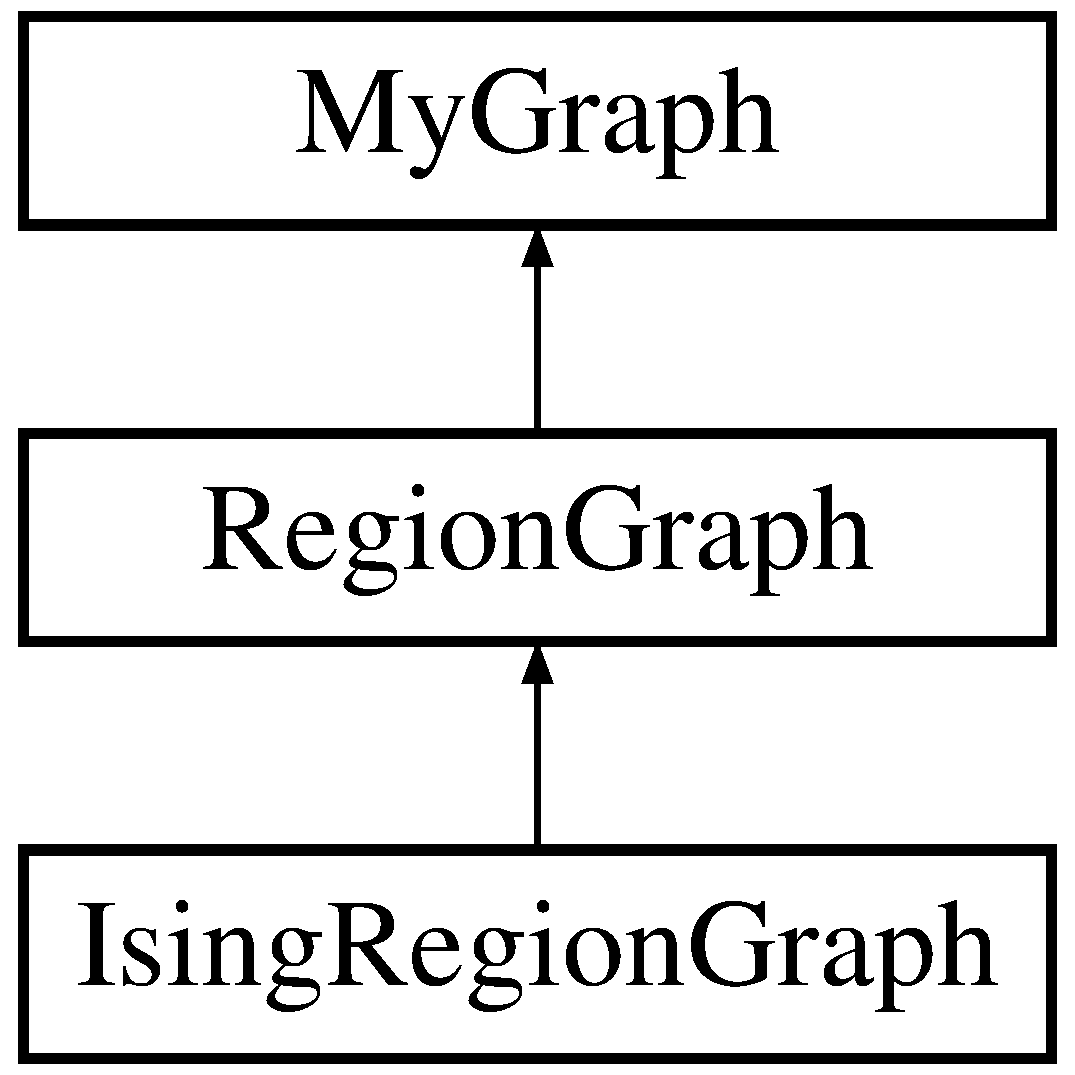
\includegraphics[height=3cm]{classRegionGraph}
\end{center}
\end{figure}
\subsection*{Public Member Functions}
\begin{CompactItemize}
\item 
{\bf RegionGraph} ({\bf FactorGraphPtr} \_\-fg)
\item 
{\bf FactorGraphPtr} {\bf getFactorGraphPtr} () const
\item 
{\bf StatePtr} {\bf getMargState} ({\bf StatePtr} sptr, {\bf RegionPtr} rgn, {\bf RegionPtr} chld)
\item 
{\bf $\sim$RegionGraph} ()
\end{CompactItemize}
\subsection*{Private Attributes}
\begin{CompactItemize}
\item 
{\bf FactorGraphPtr} {\bf graphPtr}
\end{CompactItemize}


\subsection{Detailed Description}
Graph structure for region graph implements the parent-child algorithm 



\subsection{Constructor \& Destructor Documentation}
\index{RegionGraph@{RegionGraph}!RegionGraph@{RegionGraph}}
\index{RegionGraph@{RegionGraph}!RegionGraph@{RegionGraph}}
\subsubsection{\setlength{\rightskip}{0pt plus 5cm}RegionGraph::RegionGraph ({\bf FactorGraphPtr} {\em \_\-fg})\hspace{0.3cm}{\tt  [inline]}}\label{classRegionGraph_82a3769df7050155b325787659d41336}


\index{RegionGraph@{RegionGraph}!~RegionGraph@{$\sim$RegionGraph}}
\index{~RegionGraph@{$\sim$RegionGraph}!RegionGraph@{RegionGraph}}
\subsubsection{\setlength{\rightskip}{0pt plus 5cm}RegionGraph::$\sim$RegionGraph ()\hspace{0.3cm}{\tt  [inline]}}\label{classRegionGraph_11bbe0c593aed3636f0a0aa57fdbc15e}




\subsection{Member Function Documentation}
\index{RegionGraph@{RegionGraph}!getFactorGraphPtr@{getFactorGraphPtr}}
\index{getFactorGraphPtr@{getFactorGraphPtr}!RegionGraph@{RegionGraph}}
\subsubsection{\setlength{\rightskip}{0pt plus 5cm}{\bf FactorGraphPtr} RegionGraph::getFactorGraphPtr () const\hspace{0.3cm}{\tt  [inline]}}\label{classRegionGraph_e432e4c0e4c2372560d913fd6257cd2a}


\index{RegionGraph@{RegionGraph}!getMargState@{getMargState}}
\index{getMargState@{getMargState}!RegionGraph@{RegionGraph}}
\subsubsection{\setlength{\rightskip}{0pt plus 5cm}{\bf StatePtr} RegionGraph::getMargState ({\bf StatePtr} {\em sptr}, {\bf RegionPtr} {\em rgn}, {\bf RegionPtr} {\em chld})}\label{classRegionGraph_6675c0c8ed06130a2b192466edfa271e}




\subsection{Member Data Documentation}
\index{RegionGraph@{RegionGraph}!graphPtr@{graphPtr}}
\index{graphPtr@{graphPtr}!RegionGraph@{RegionGraph}}
\subsubsection{\setlength{\rightskip}{0pt plus 5cm}{\bf FactorGraphPtr} {\bf RegionGraph::graphPtr}\hspace{0.3cm}{\tt  [private]}}\label{classRegionGraph_7dad8406a69860b74ab83e3153cf57ac}




Reimplemented in {\bf IsingRegionGraph} \doxyref{}{p.}{classIsingRegionGraph_66bffb3f21f7597e2dfa5027eae7d7e8}.

The documentation for this class was generated from the following files:\begin{CompactItemize}
\item 
inc/{\bf mygraph.h}\item 
src/{\bf mygraph.cpp}\end{CompactItemize}

\section{RegionPPM Class Reference}
\label{classRegionPPM}\index{RegionPPM@{RegionPPM}}
{\tt \#include $<$RegionPPM.h$>$}

Inheritance diagram for RegionPPM::\begin{figure}[H]
\begin{center}
\leavevmode
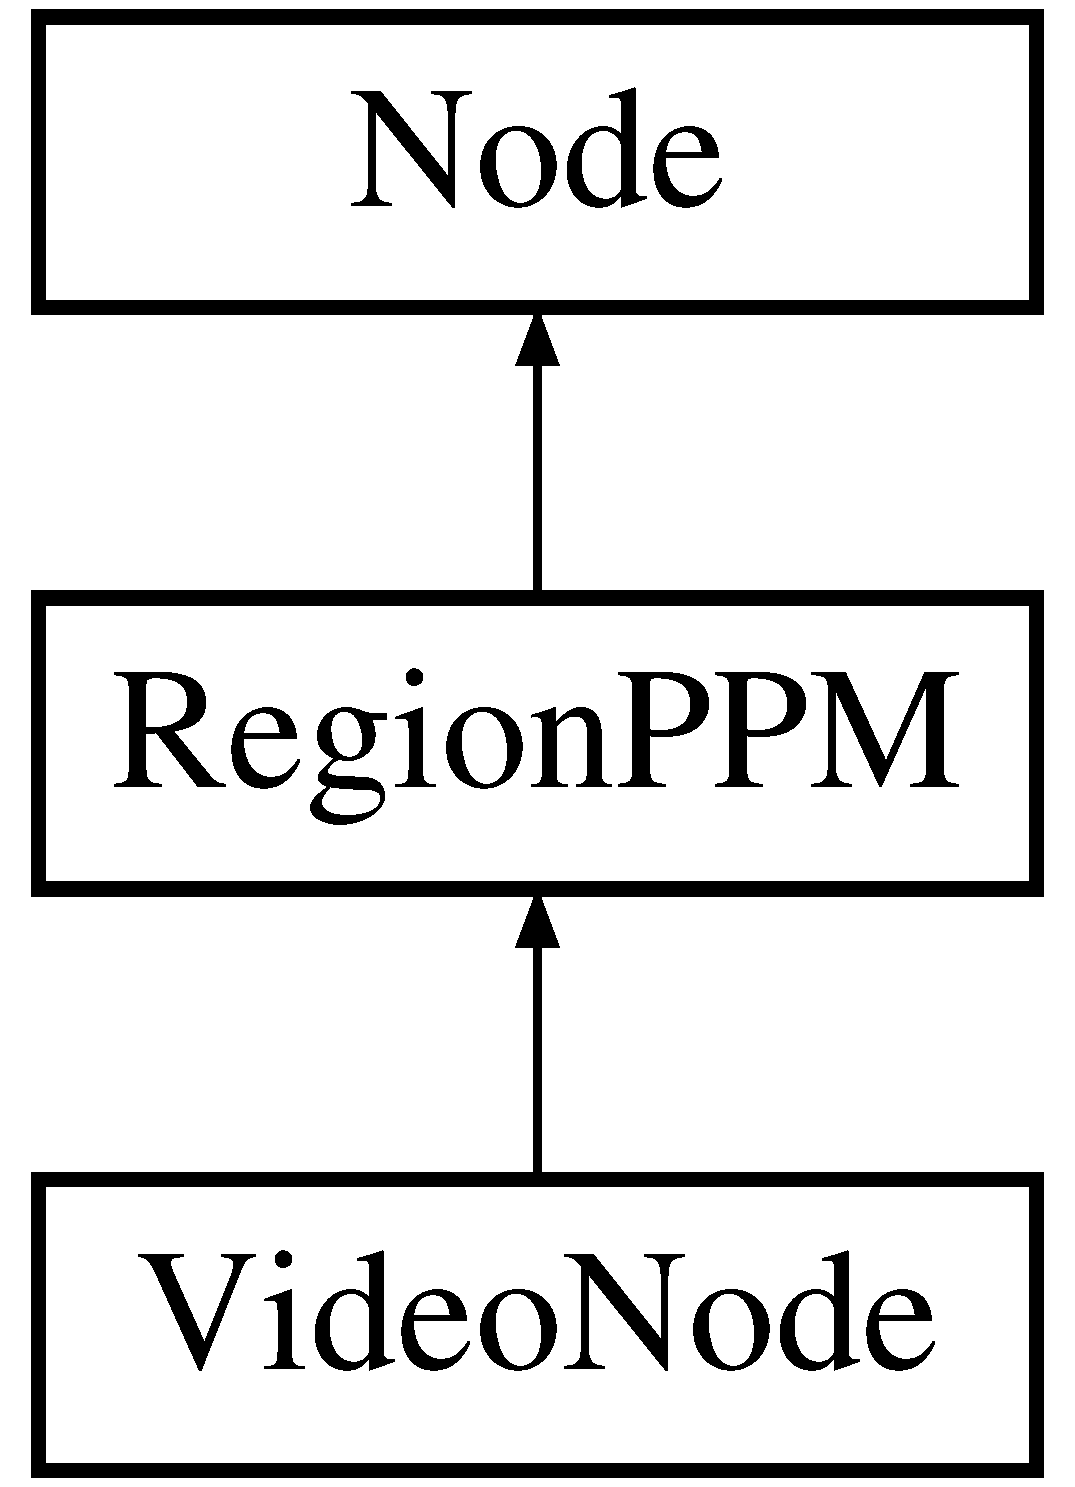
\includegraphics[height=3cm]{classRegionPPM}
\end{center}
\end{figure}
\subsection*{Public Member Functions}
\begin{CompactItemize}
\item 
{\bf RegionPPM} (string s, int {\bf numVar}, {\bf Belief} $\ast$bp=0, int \_\-type=-1)
\item 
void {\bf setCR} (int \_\-cr)
\item 
int {\bf getCR} ()
\item 
void {\bf clear} ()
\item 
{\bf $\sim$RegionPPM} ()
\end{CompactItemize}
\subsection*{Public Attributes}
\begin{CompactItemize}
\item 
{\bf LD} {\bf m\_\-alpha}
\begin{CompactList}\small\item\em single normalizing factor $m_\alpha$ for region $\alpha$ \item\end{CompactList}\item 
{\bf BeliefPtr} {\bf lambdaR}
\begin{CompactList}\small\item\em normalizing factor per initial state used by \doxyref{GraphPPM}{p.}{classGraphPPM} \item\end{CompactList}\item 
{\bf ConditionalBeliefPtr} {\bf pHat}
\begin{CompactList}\small\item\em the conditional evolution model used by \doxyref{GraphGBP}{p.}{classGraphGBP} \& \doxyref{GraphPPM}{p.}{classGraphPPM} \item\end{CompactList}\item 
{\bf ConditionalBeliefPtr} {\bf bJointRev}
\begin{CompactList}\small\item\em new values for $b_\alpha^{t, t+\delta t}$ saved as $t+\delta t, t$ (in reverse) \item\end{CompactList}\item 
{\bf BeliefPtr} {\bf bNew}
\begin{CompactList}\small\item\em the new beliefs which are committed to region beliefs at commit stage \item\end{CompactList}\item 
{\bf BeliefPtr} {\bf bLast}
\begin{CompactList}\small\item\em record holder for last beliefs \item\end{CompactList}\item 
{\bf ConditionalBeliefPtr} {\bf lambdaPar}
\begin{CompactList}\small\item\em Holds all alpha-$>$parent contributions per alpha state, used by \doxyref{GraphPPM}{p.}{classGraphPPM}. \item\end{CompactList}\item 
{\bf ConditionalBeliefPtr} {\bf lambdaChild}
\begin{CompactList}\small\item\em Holds all child-$>$alpha per alpha state (computed using child reduced state messages). \item\end{CompactList}\item 
{\bf LD} {\bf avgDevFromPar}
\begin{CompactList}\small\item\em average(over all states) deviation in belief compared with parent normalized beliefs \item\end{CompactList}\item 
{\bf LD} {\bf avgChngInBlfs}
\begin{CompactList}\small\item\em average(over all states) change in the belief compared with last iteration beliefs \item\end{CompactList}\item 
{\bf LD} {\bf maxChngInBlfs}
\begin{CompactList}\small\item\em maximum deviation in belief compared with parent normalized beliefs \item\end{CompactList}\item 
{\bf LD} {\bf maxDevFromPar}
\begin{CompactList}\small\item\em maximum(over all states) change in the belief compared with last iteration beliefs \item\end{CompactList}\item 
{\bf LD} {\bf SR}
\begin{CompactList}\small\item\em region entropy \item\end{CompactList}\end{CompactItemize}
\subsection*{Private Attributes}
\begin{CompactItemize}
\item 
int {\bf cr}
\end{CompactItemize}


\subsection{Detailed Description}
Modification of \doxyref{GraphPPM.h}{p.}{GraphPPM_8h} to a separate class -used by both \doxyref{GraphPPM}{p.}{classGraphPPM} and \doxyref{GraphGBP}{p.}{classGraphGBP} 



\subsection{Constructor \& Destructor Documentation}
\index{RegionPPM@{RegionPPM}!RegionPPM@{RegionPPM}}
\index{RegionPPM@{RegionPPM}!RegionPPM@{RegionPPM}}
\subsubsection{\setlength{\rightskip}{0pt plus 5cm}RegionPPM::RegionPPM (string {\em s}, int {\em numVar}, {\bf Belief} $\ast$ {\em bp} = {\tt 0}, int {\em \_\-type} = {\tt -1})\hspace{0.3cm}{\tt  [inline]}}\label{classRegionPPM_659495288448a7dc88dcbbe0e9ce0185}


\index{RegionPPM@{RegionPPM}!~RegionPPM@{$\sim$RegionPPM}}
\index{~RegionPPM@{$\sim$RegionPPM}!RegionPPM@{RegionPPM}}
\subsubsection{\setlength{\rightskip}{0pt plus 5cm}RegionPPM::$\sim$RegionPPM ()\hspace{0.3cm}{\tt  [inline]}}\label{classRegionPPM_c49230d225cdff2b0fe9fcf646e5dc77}




\subsection{Member Function Documentation}
\index{RegionPPM@{RegionPPM}!setCR@{setCR}}
\index{setCR@{setCR}!RegionPPM@{RegionPPM}}
\subsubsection{\setlength{\rightskip}{0pt plus 5cm}void RegionPPM::setCR (int {\em \_\-cr})\hspace{0.3cm}{\tt  [inline]}}\label{classRegionPPM_bf2b481562fb2fd4b367a9fdf81c2cb6}


\index{RegionPPM@{RegionPPM}!getCR@{getCR}}
\index{getCR@{getCR}!RegionPPM@{RegionPPM}}
\subsubsection{\setlength{\rightskip}{0pt plus 5cm}int RegionPPM::getCR ()\hspace{0.3cm}{\tt  [inline]}}\label{classRegionPPM_2787a87dbf3ad30e961e8ff413361104}


\index{RegionPPM@{RegionPPM}!clear@{clear}}
\index{clear@{clear}!RegionPPM@{RegionPPM}}
\subsubsection{\setlength{\rightskip}{0pt plus 5cm}void RegionPPM::clear ()\hspace{0.3cm}{\tt  [inline]}}\label{classRegionPPM_660d657bb86f6c374248c0f2f63b38ca}




\subsection{Member Data Documentation}
\index{RegionPPM@{RegionPPM}!cr@{cr}}
\index{cr@{cr}!RegionPPM@{RegionPPM}}
\subsubsection{\setlength{\rightskip}{0pt plus 5cm}int {\bf RegionPPM::cr}\hspace{0.3cm}{\tt  [private]}}\label{classRegionPPM_c21f25cb3cd95ae5717909badbb7014a}




Reimplemented in {\bf VideoNode} \doxyref{}{p.}{classVideoNode_07fc09cceeaf0bfef6690aecdb2a5574}.\index{RegionPPM@{RegionPPM}!m_alpha@{m\_\-alpha}}
\index{m_alpha@{m\_\-alpha}!RegionPPM@{RegionPPM}}
\subsubsection{\setlength{\rightskip}{0pt plus 5cm}{\bf LD} {\bf RegionPPM::m\_\-alpha}}\label{classRegionPPM_130c2c0a956e9d3c552593f5ab3a178f}


single normalizing factor $m_\alpha$ for region $\alpha$ 

\index{RegionPPM@{RegionPPM}!lambdaR@{lambdaR}}
\index{lambdaR@{lambdaR}!RegionPPM@{RegionPPM}}
\subsubsection{\setlength{\rightskip}{0pt plus 5cm}{\bf BeliefPtr} {\bf RegionPPM::lambdaR}}\label{classRegionPPM_14fc4409c5e6da29e3f6d312bab54d8d}


normalizing factor per initial state used by \doxyref{GraphPPM}{p.}{classGraphPPM} 

\index{RegionPPM@{RegionPPM}!pHat@{pHat}}
\index{pHat@{pHat}!RegionPPM@{RegionPPM}}
\subsubsection{\setlength{\rightskip}{0pt plus 5cm}{\bf ConditionalBeliefPtr} {\bf RegionPPM::pHat}}\label{classRegionPPM_106816e785642f479cb77a74d091fa4d}


the conditional evolution model used by \doxyref{GraphGBP}{p.}{classGraphGBP} \& \doxyref{GraphPPM}{p.}{classGraphPPM} 

\index{RegionPPM@{RegionPPM}!bJointRev@{bJointRev}}
\index{bJointRev@{bJointRev}!RegionPPM@{RegionPPM}}
\subsubsection{\setlength{\rightskip}{0pt plus 5cm}{\bf ConditionalBeliefPtr} {\bf RegionPPM::bJointRev}}\label{classRegionPPM_ae56fc025e98f6e03a8714c0c1b7d59b}


new values for $b_\alpha^{t, t+\delta t}$ saved as $t+\delta t, t$ (in reverse) 

\index{RegionPPM@{RegionPPM}!bNew@{bNew}}
\index{bNew@{bNew}!RegionPPM@{RegionPPM}}
\subsubsection{\setlength{\rightskip}{0pt plus 5cm}{\bf BeliefPtr} {\bf RegionPPM::bNew}}\label{classRegionPPM_780ea2790c72badf9582019167327a22}


the new beliefs which are committed to region beliefs at commit stage 

\index{RegionPPM@{RegionPPM}!bLast@{bLast}}
\index{bLast@{bLast}!RegionPPM@{RegionPPM}}
\subsubsection{\setlength{\rightskip}{0pt plus 5cm}{\bf BeliefPtr} {\bf RegionPPM::bLast}}\label{classRegionPPM_727bb4f713b3c059e0c9c106f7603c9c}


record holder for last beliefs 

\index{RegionPPM@{RegionPPM}!lambdaPar@{lambdaPar}}
\index{lambdaPar@{lambdaPar}!RegionPPM@{RegionPPM}}
\subsubsection{\setlength{\rightskip}{0pt plus 5cm}{\bf ConditionalBeliefPtr} {\bf RegionPPM::lambdaPar}}\label{classRegionPPM_cfeeb2e142bfd0389e25dcf16ddb9369}


Holds all alpha-$>$parent contributions per alpha state, used by \doxyref{GraphPPM}{p.}{classGraphPPM}. 

\index{RegionPPM@{RegionPPM}!lambdaChild@{lambdaChild}}
\index{lambdaChild@{lambdaChild}!RegionPPM@{RegionPPM}}
\subsubsection{\setlength{\rightskip}{0pt plus 5cm}{\bf ConditionalBeliefPtr} {\bf RegionPPM::lambdaChild}}\label{classRegionPPM_5c299f6aeafbabe1f3a0f2aa72598a32}


Holds all child-$>$alpha per alpha state (computed using child reduced state messages). 

\index{RegionPPM@{RegionPPM}!avgDevFromPar@{avgDevFromPar}}
\index{avgDevFromPar@{avgDevFromPar}!RegionPPM@{RegionPPM}}
\subsubsection{\setlength{\rightskip}{0pt plus 5cm}{\bf LD} {\bf RegionPPM::avgDevFromPar}}\label{classRegionPPM_48d041918dbd4d3f5cd4510cf9fd1a99}


average(over all states) deviation in belief compared with parent normalized beliefs 

\index{RegionPPM@{RegionPPM}!avgChngInBlfs@{avgChngInBlfs}}
\index{avgChngInBlfs@{avgChngInBlfs}!RegionPPM@{RegionPPM}}
\subsubsection{\setlength{\rightskip}{0pt plus 5cm}{\bf LD} {\bf RegionPPM::avgChngInBlfs}}\label{classRegionPPM_63cca40544ca1627867e540881fd548e}


average(over all states) change in the belief compared with last iteration beliefs 

\index{RegionPPM@{RegionPPM}!maxChngInBlfs@{maxChngInBlfs}}
\index{maxChngInBlfs@{maxChngInBlfs}!RegionPPM@{RegionPPM}}
\subsubsection{\setlength{\rightskip}{0pt plus 5cm}{\bf LD} {\bf RegionPPM::maxChngInBlfs}}\label{classRegionPPM_0154611b5fa4784a633276dcb5222eb4}


maximum deviation in belief compared with parent normalized beliefs 

\index{RegionPPM@{RegionPPM}!maxDevFromPar@{maxDevFromPar}}
\index{maxDevFromPar@{maxDevFromPar}!RegionPPM@{RegionPPM}}
\subsubsection{\setlength{\rightskip}{0pt plus 5cm}{\bf LD} {\bf RegionPPM::maxDevFromPar}}\label{classRegionPPM_0d7aafa2ad48ada73955b3a1250a5c3a}


maximum(over all states) change in the belief compared with last iteration beliefs 

\index{RegionPPM@{RegionPPM}!SR@{SR}}
\index{SR@{SR}!RegionPPM@{RegionPPM}}
\subsubsection{\setlength{\rightskip}{0pt plus 5cm}{\bf LD} {\bf RegionPPM::SR}}\label{classRegionPPM_3c9865b0a3610a4ab72704386dc7b1af}


region entropy 



The documentation for this class was generated from the following file:\begin{CompactItemize}
\item 
inc/{\bf RegionPPM.h}\end{CompactItemize}

\section{RgbPixel Struct Reference}
\label{structRgbPixel}\index{RgbPixel@{RgbPixel}}
{\tt \#include $<$Image.h$>$}

\subsection*{Public Attributes}
\begin{CompactItemize}
\item 
unsigned char {\bf b}
\item 
unsigned char {\bf g}
\item 
unsigned char {\bf r}
\end{CompactItemize}


\subsection{Member Data Documentation}
\index{RgbPixel@{RgbPixel}!b@{b}}
\index{b@{b}!RgbPixel@{RgbPixel}}
\subsubsection{\setlength{\rightskip}{0pt plus 5cm}unsigned char {\bf RgbPixel::b}}\label{structRgbPixel_7328feddcf5c0f6161e142d5e5195f5d}


\index{RgbPixel@{RgbPixel}!g@{g}}
\index{g@{g}!RgbPixel@{RgbPixel}}
\subsubsection{\setlength{\rightskip}{0pt plus 5cm}unsigned char {\bf RgbPixel::g}}\label{structRgbPixel_c2fc04f5b5918f8649e3594829cdb172}


\index{RgbPixel@{RgbPixel}!r@{r}}
\index{r@{r}!RgbPixel@{RgbPixel}}
\subsubsection{\setlength{\rightskip}{0pt plus 5cm}unsigned char {\bf RgbPixel::r}}\label{structRgbPixel_0ab07798c8be7b2bdab0c0346edc640c}




The documentation for this struct was generated from the following file:\begin{CompactItemize}
\item 
inc/{\bf Image.h}\end{CompactItemize}

\section{RgbPixelFloat Struct Reference}
\label{structRgbPixelFloat}\index{RgbPixelFloat@{RgbPixelFloat}}
{\tt \#include $<$Image.h$>$}

\subsection*{Public Attributes}
\begin{CompactItemize}
\item 
float {\bf b}
\item 
float {\bf g}
\item 
float {\bf r}
\end{CompactItemize}


\subsection{Member Data Documentation}
\index{RgbPixelFloat@{RgbPixelFloat}!b@{b}}
\index{b@{b}!RgbPixelFloat@{RgbPixelFloat}}
\subsubsection{\setlength{\rightskip}{0pt plus 5cm}float {\bf RgbPixelFloat::b}}\label{structRgbPixelFloat_97cdd6c61c87fed8ffcc4492c3f5de2d}


\index{RgbPixelFloat@{RgbPixelFloat}!g@{g}}
\index{g@{g}!RgbPixelFloat@{RgbPixelFloat}}
\subsubsection{\setlength{\rightskip}{0pt plus 5cm}float {\bf RgbPixelFloat::g}}\label{structRgbPixelFloat_6f04fa6799f1e67072b3d53aed318d0f}


\index{RgbPixelFloat@{RgbPixelFloat}!r@{r}}
\index{r@{r}!RgbPixelFloat@{RgbPixelFloat}}
\subsubsection{\setlength{\rightskip}{0pt plus 5cm}float {\bf RgbPixelFloat::r}}\label{structRgbPixelFloat_b4fc0f3ef850578208e95a334fa8f3c2}




The documentation for this struct was generated from the following file:\begin{CompactItemize}
\item 
inc/{\bf Image.h}\end{CompactItemize}

\section{SPLD\_\-Cmp Struct Reference}
\label{structSPLD__Cmp}\index{SPLD_Cmp@{SPLD\_\-Cmp}}
{\tt \#include $<$state.h$>$}

\subsection*{Public Member Functions}
\begin{CompactItemize}
\item 
{\bf SPLD\_\-Cmp} (bool ch=true)
\item 
bool {\bf operator()} (const pair$<$ {\bf StatePtr}, {\bf LD} $>$ \&p1, const pair$<$ {\bf StatePtr}, {\bf LD} $>$ \&p2) const
\end{CompactItemize}
\subsection*{Public Attributes}
\begin{CompactItemize}
\item 
bool {\bf choice}
\end{CompactItemize}


\subsection{Constructor \& Destructor Documentation}
\index{SPLD_Cmp@{SPLD\_\-Cmp}!SPLD_Cmp@{SPLD\_\-Cmp}}
\index{SPLD_Cmp@{SPLD\_\-Cmp}!SPLD_Cmp@{SPLD\_\-Cmp}}
\subsubsection{\setlength{\rightskip}{0pt plus 5cm}SPLD\_\-Cmp::SPLD\_\-Cmp (bool {\em ch} = {\tt true})\hspace{0.3cm}{\tt  [inline]}}\label{structSPLD__Cmp_514695faf99dce5d85134029ec6740a1}




\subsection{Member Function Documentation}
\index{SPLD_Cmp@{SPLD\_\-Cmp}!operator()@{operator()}}
\index{operator()@{operator()}!SPLD_Cmp@{SPLD\_\-Cmp}}
\subsubsection{\setlength{\rightskip}{0pt plus 5cm}bool SPLD\_\-Cmp::operator() (const pair$<$ {\bf StatePtr}, {\bf LD} $>$ \& {\em p1}, const pair$<$ {\bf StatePtr}, {\bf LD} $>$ \& {\em p2}) const\hspace{0.3cm}{\tt  [inline]}}\label{structSPLD__Cmp_577102fd5f0c4104da8ecf3d71eb63d9}




\subsection{Member Data Documentation}
\index{SPLD_Cmp@{SPLD\_\-Cmp}!choice@{choice}}
\index{choice@{choice}!SPLD_Cmp@{SPLD\_\-Cmp}}
\subsubsection{\setlength{\rightskip}{0pt plus 5cm}bool {\bf SPLD\_\-Cmp::choice}}\label{structSPLD__Cmp_9566f4b0879a98e641c4b5a0dc93cfd9}




The documentation for this struct was generated from the following file:\begin{CompactItemize}
\item 
inc/{\bf state.h}\end{CompactItemize}

\section{State Class Reference}
\label{classState}\index{State@{State}}
{\tt \#include $<$state.h$>$}

\subsection*{Public Member Functions}
\begin{CompactItemize}
\item 
{\bf State} (int \_\-n, {\bf INT} $\ast$\_\-d)
\item 
{\bf State} (vector$<$ {\bf INT} $>$ v)
\item 
{\bf State} (const {\bf State} \&st2)
\item 
bool {\bf operator==} (const {\bf State} \&s2) const 
\item 
{\bf INT} {\bf getData} (int idx) const
\item 
{\bf State} {\bf operator+} (const {\bf State} \&s2) const 
\item 
{\bf $\sim$State} ()
\item 
{\bf VI} {\bf getVec} ()
\end{CompactItemize}
\subsection*{Static Public Member Functions}
\begin{CompactItemize}
\item 
static {\bf LD} {\bf SSD} ({\bf State} \&s1, {\bf State} \&s2)
\end{CompactItemize}
\subsection*{Public Attributes}
\begin{CompactItemize}
\item 
int {\bf num}
\item 
{\bf INT} $\ast$ {\bf data}
\end{CompactItemize}
\subsection*{Friends}
\begin{CompactItemize}
\item 
ostream \& {\bf operator$<$$<$} (ostream \&os, {\bf State} \&s)
\end{CompactItemize}


\subsection{Constructor \& Destructor Documentation}
\index{State@{State}!State@{State}}
\index{State@{State}!State@{State}}
\subsubsection{\setlength{\rightskip}{0pt plus 5cm}State::State (int {\em \_\-n}, {\bf INT} $\ast$ {\em \_\-d})\hspace{0.3cm}{\tt  [inline]}}\label{classState_0ef5c563f639f788f24afbc7f0f37288}


\index{State@{State}!State@{State}}
\index{State@{State}!State@{State}}
\subsubsection{\setlength{\rightskip}{0pt plus 5cm}State::State (vector$<$ {\bf INT} $>$ {\em v})\hspace{0.3cm}{\tt  [inline]}}\label{classState_c4fc0df913015a99774456669f2bdaa1}


\index{State@{State}!State@{State}}
\index{State@{State}!State@{State}}
\subsubsection{\setlength{\rightskip}{0pt plus 5cm}State::State (const {\bf State} \& {\em st2})\hspace{0.3cm}{\tt  [inline]}}\label{classState_0261bbf902290f544599c70e2951a80c}


\index{State@{State}!~State@{$\sim$State}}
\index{~State@{$\sim$State}!State@{State}}
\subsubsection{\setlength{\rightskip}{0pt plus 5cm}State::$\sim$State ()\hspace{0.3cm}{\tt  [inline]}}\label{classState_4996784dd93206fc1cb99ca51c4725dd}




\subsection{Member Function Documentation}
\index{State@{State}!SSD@{SSD}}
\index{SSD@{SSD}!State@{State}}
\subsubsection{\setlength{\rightskip}{0pt plus 5cm}{\bf LD} State::SSD ({\bf State} \& {\em s1}, {\bf State} \& {\em s2})\hspace{0.3cm}{\tt  [static]}}\label{classState_ee08b1dc453489f8482702edb8300a75}


\index{State@{State}!operator==@{operator==}}
\index{operator==@{operator==}!State@{State}}
\subsubsection{\setlength{\rightskip}{0pt plus 5cm}bool State::operator== (const {\bf State} \& {\em s2}) const\hspace{0.3cm}{\tt  [inline]}}\label{classState_022d012312dbd1c3cb170e752a4cc726}


\index{State@{State}!getData@{getData}}
\index{getData@{getData}!State@{State}}
\subsubsection{\setlength{\rightskip}{0pt plus 5cm}{\bf INT} State::getData (int {\em idx}) const\hspace{0.3cm}{\tt  [inline]}}\label{classState_2b022e8fcebaec720672e42fde918337}


\index{State@{State}!operator+@{operator+}}
\index{operator+@{operator+}!State@{State}}
\subsubsection{\setlength{\rightskip}{0pt plus 5cm}{\bf State} State::operator+ (const {\bf State} \& {\em s2}) const\hspace{0.3cm}{\tt  [inline]}}\label{classState_41cf21cb4c380e045a360b7061f8da73}


\index{State@{State}!getVec@{getVec}}
\index{getVec@{getVec}!State@{State}}
\subsubsection{\setlength{\rightskip}{0pt plus 5cm}{\bf VI} State::getVec ()\hspace{0.3cm}{\tt  [inline]}}\label{classState_a37002bfd280361ce414b6c7ee97ef47}




\subsection{Friends And Related Function Documentation}
\index{State@{State}!operator<<@{operator$<$$<$}}
\index{operator<<@{operator$<$$<$}!State@{State}}
\subsubsection{\setlength{\rightskip}{0pt plus 5cm}ostream\& operator$<$$<$ (ostream \& {\em os}, {\bf State} \& {\em s})\hspace{0.3cm}{\tt  [friend]}}\label{classState_29d139259ad178fd96a89e26b2901cbe}




\subsection{Member Data Documentation}
\index{State@{State}!num@{num}}
\index{num@{num}!State@{State}}
\subsubsection{\setlength{\rightskip}{0pt plus 5cm}int {\bf State::num}}\label{classState_2091da71db2bcf6df658fd16c905c716}


\index{State@{State}!data@{data}}
\index{data@{data}!State@{State}}
\subsubsection{\setlength{\rightskip}{0pt plus 5cm}{\bf INT}$\ast$ {\bf State::data}}\label{classState_0f5a8a0a362d302a11e5ee1396e876b3}




The documentation for this class was generated from the following files:\begin{CompactItemize}
\item 
inc/{\bf state.h}\item 
src/{\bf state.cpp}\end{CompactItemize}

\section{StatePtrCmp Struct Reference}
\label{structStatePtrCmp}\index{StatePtrCmp@{StatePtrCmp}}
{\tt \#include $<$state.h$>$}

\subsection*{Public Member Functions}
\begin{CompactItemize}
\item 
bool {\bf operator()} (const {\bf StatePtr} \&sp1, const {\bf StatePtr} \&sp2) const
\end{CompactItemize}


\subsection{Member Function Documentation}
\index{StatePtrCmp@{StatePtrCmp}!operator()@{operator()}}
\index{operator()@{operator()}!StatePtrCmp@{StatePtrCmp}}
\subsubsection{\setlength{\rightskip}{0pt plus 5cm}bool StatePtrCmp::operator() (const {\bf StatePtr} \& {\em sp1}, const {\bf StatePtr} \& {\em sp2}) const\hspace{0.3cm}{\tt  [inline]}}\label{structStatePtrCmp_d5c4022bf6d89676239513e6e228833f}




The documentation for this struct was generated from the following file:\begin{CompactItemize}
\item 
inc/{\bf state.h}\end{CompactItemize}

\section{StGBP Class Reference}
\label{classStGBP}\index{StGBP@{StGBP}}
{\tt \#include $<$stGBP.h$>$}

\subsection*{Private Attributes}
\begin{CompactItemize}
\item 
{\bf PottsModel} $\ast$ {\bf model}
\begin{CompactList}\small\item\em the model - this is common across the \item\end{CompactList}\end{CompactItemize}


\subsection{Detailed Description}
This class implements the single multiple iteration space-time GBP. 



\subsection{Member Data Documentation}
\index{StGBP@{StGBP}!model@{model}}
\index{model@{model}!StGBP@{StGBP}}
\subsubsection{\setlength{\rightskip}{0pt plus 5cm}{\bf PottsModel}$\ast$ {\bf StGBP::model}\hspace{0.3cm}{\tt  [private]}}\label{classStGBP_918b5cba3de8b98d0fcafc8a357bd922}


the model - this is common across the 



The documentation for this class was generated from the following file:\begin{CompactItemize}
\item 
inc/{\bf stGBP.h}\end{CompactItemize}

\section{Timer Class Reference}
\label{classTimer}\index{Timer@{Timer}}
{\tt \#include $<$main.h$>$}

\subsection*{Public Member Functions}
\begin{CompactItemize}
\item 
{\bf Timer} (int \_\-incr=1, FILE $\ast$\_\-fout=stderr)
\item 
void {\bf tick} ()
\item 
double {\bf getElapsed} ()
\end{CompactItemize}
\subsection*{Private Attributes}
\begin{CompactItemize}
\item 
time\_\-t {\bf tb}
\item 
double {\bf last}
\item 
int {\bf incr}
\item 
FILE $\ast$ {\bf fout}
\end{CompactItemize}


\subsection{Constructor \& Destructor Documentation}
\index{Timer@{Timer}!Timer@{Timer}}
\index{Timer@{Timer}!Timer@{Timer}}
\subsubsection{\setlength{\rightskip}{0pt plus 5cm}Timer::Timer (int {\em \_\-incr} = {\tt 1}, FILE $\ast$ {\em \_\-fout} = {\tt stderr})\hspace{0.3cm}{\tt  [inline]}}\label{classTimer_85dad19b57140a177e64a2b47a08bb3c}




\subsection{Member Function Documentation}
\index{Timer@{Timer}!tick@{tick}}
\index{tick@{tick}!Timer@{Timer}}
\subsubsection{\setlength{\rightskip}{0pt plus 5cm}void Timer::tick ()\hspace{0.3cm}{\tt  [inline]}}\label{classTimer_38076ccaf3684782b008dfeb9a1659e3}


\index{Timer@{Timer}!getElapsed@{getElapsed}}
\index{getElapsed@{getElapsed}!Timer@{Timer}}
\subsubsection{\setlength{\rightskip}{0pt plus 5cm}double Timer::getElapsed ()\hspace{0.3cm}{\tt  [inline]}}\label{classTimer_6d22efbd1f3ae9a3dd975dcfb033db66}




\subsection{Member Data Documentation}
\index{Timer@{Timer}!tb@{tb}}
\index{tb@{tb}!Timer@{Timer}}
\subsubsection{\setlength{\rightskip}{0pt plus 5cm}time\_\-t {\bf Timer::tb}\hspace{0.3cm}{\tt  [private]}}\label{classTimer_3b0d6c90e75035d605965c8117bcd4f8}


\index{Timer@{Timer}!last@{last}}
\index{last@{last}!Timer@{Timer}}
\subsubsection{\setlength{\rightskip}{0pt plus 5cm}double {\bf Timer::last}\hspace{0.3cm}{\tt  [private]}}\label{classTimer_348f0b583fa3b3d5f720e826d07d65fe}


\index{Timer@{Timer}!incr@{incr}}
\index{incr@{incr}!Timer@{Timer}}
\subsubsection{\setlength{\rightskip}{0pt plus 5cm}int {\bf Timer::incr}\hspace{0.3cm}{\tt  [private]}}\label{classTimer_4ae63194f3b00f8295e27e53f9ce883c}


\index{Timer@{Timer}!fout@{fout}}
\index{fout@{fout}!Timer@{Timer}}
\subsubsection{\setlength{\rightskip}{0pt plus 5cm}FILE$\ast$ {\bf Timer::fout}\hspace{0.3cm}{\tt  [private]}}\label{classTimer_79206658889015a54bd4495110f0cc70}




The documentation for this class was generated from the following file:\begin{CompactItemize}
\item 
inc/{\bf main.h}\end{CompactItemize}

\section{Tracker Class Reference}
\label{classTracker}\index{Tracker@{Tracker}}
{\tt \#include $<$Tracker.h$>$}

\subsection*{Public Member Functions}
\begin{CompactItemize}
\item 
{\bf Tracker} ()
\item 
void {\bf initMain} (string videoName, int NL, bool isGray, int {\bf C}, {\bf LD} {\bf theta}, int rx, int ry, int cx, int cy)
\item 
void {\bf initGraph} (int rx, int ry, int cx, int cy)
\item 
void {\bf initVideo} (string videoName, int NL, bool isGray)
\item 
void {\bf run} (int priorNum, int maxNum, int frameJump)
\item 
IplImage $\ast$ {\bf getFrameDiff} (IplImage $\ast$frame1, IplImage $\ast$frame2)
\item 
void {\bf updateModel} (IplImage $\ast$prev\_\-frame, IplImage $\ast$next\_\-frame)
\item 
bool {\bf updateFrame} ()
\item 
IplImage $\ast$ {\bf greedyFillFrame} ()
\item 
void {\bf run\_\-step} ({\bf LD} {\bf theta}, {\bf LD} dt)
\end{CompactItemize}
\subsection*{Private Attributes}
\begin{CompactItemize}
\item 
int {\bf N2}
\item 
int {\bf N1}
\item 
int {\bf counter}
\item 
{\bf PottsModel} $\ast$ {\bf model}
\item 
{\bf PottsGraphPPM} $\ast$ {\bf graph}
\item 
{\bf VideoReader} $\ast$ {\bf vreader}
\item 
int {\bf C}
\item 
{\bf LD} {\bf epsilon}
\item 
{\bf LD} {\bf theta}
\item 
IplImage $\ast$ {\bf last\_\-frame}
\item 
IplImage $\ast$ {\bf curr\_\-frame}
\item 
IplImage $\ast$ {\bf track\_\-frame}
\end{CompactItemize}


\subsection{Constructor \& Destructor Documentation}
\index{Tracker@{Tracker}!Tracker@{Tracker}}
\index{Tracker@{Tracker}!Tracker@{Tracker}}
\subsubsection{\setlength{\rightskip}{0pt plus 5cm}Tracker::Tracker ()}\label{classTracker_6ac188cc1a7bc78c9c23fa35cfa2742d}




\subsection{Member Function Documentation}
\index{Tracker@{Tracker}!initMain@{initMain}}
\index{initMain@{initMain}!Tracker@{Tracker}}
\subsubsection{\setlength{\rightskip}{0pt plus 5cm}void Tracker::initMain (string {\em videoName}, int {\em NL}, bool {\em isGray}, int {\em C}, {\bf LD} {\em theta}, int {\em rx}, int {\em ry}, int {\em cx}, int {\em cy})}\label{classTracker_91e80d80282f05cfd44b4afbf930d115}


\index{Tracker@{Tracker}!initGraph@{initGraph}}
\index{initGraph@{initGraph}!Tracker@{Tracker}}
\subsubsection{\setlength{\rightskip}{0pt plus 5cm}void Tracker::initGraph (int {\em rx}, int {\em ry}, int {\em cx}, int {\em cy})}\label{classTracker_091a2a46637eefac94dc2ce2ce01055a}


\index{Tracker@{Tracker}!initVideo@{initVideo}}
\index{initVideo@{initVideo}!Tracker@{Tracker}}
\subsubsection{\setlength{\rightskip}{0pt plus 5cm}void Tracker::initVideo (string {\em videoName}, int {\em NL}, bool {\em isGray})}\label{classTracker_fed96a3c5ef6f91e1a7414044fb32ccd}


\index{Tracker@{Tracker}!run@{run}}
\index{run@{run}!Tracker@{Tracker}}
\subsubsection{\setlength{\rightskip}{0pt plus 5cm}void Tracker::run (int {\em priorNum}, int {\em maxNum}, int {\em frameJump})}\label{classTracker_c14d6b9659cf4d843d38ac013a33c6ba}


\index{Tracker@{Tracker}!getFrameDiff@{getFrameDiff}}
\index{getFrameDiff@{getFrameDiff}!Tracker@{Tracker}}
\subsubsection{\setlength{\rightskip}{0pt plus 5cm}IplImage$\ast$ Tracker::getFrameDiff (IplImage $\ast$ {\em frame1}, IplImage $\ast$ {\em frame2})}\label{classTracker_67809409f88f4384220c128e9ddbec15}


\index{Tracker@{Tracker}!updateModel@{updateModel}}
\index{updateModel@{updateModel}!Tracker@{Tracker}}
\subsubsection{\setlength{\rightskip}{0pt plus 5cm}void Tracker::updateModel (IplImage $\ast$ {\em prev\_\-frame}, IplImage $\ast$ {\em next\_\-frame})}\label{classTracker_991ce3039007bfc315a8feef77b88ed0}


\index{Tracker@{Tracker}!updateFrame@{updateFrame}}
\index{updateFrame@{updateFrame}!Tracker@{Tracker}}
\subsubsection{\setlength{\rightskip}{0pt plus 5cm}bool Tracker::updateFrame ()}\label{classTracker_658a9c0a99c9c0c69034be9772b23921}


\index{Tracker@{Tracker}!greedyFillFrame@{greedyFillFrame}}
\index{greedyFillFrame@{greedyFillFrame}!Tracker@{Tracker}}
\subsubsection{\setlength{\rightskip}{0pt plus 5cm}IplImage$\ast$ Tracker::greedyFillFrame ()}\label{classTracker_36a43fe254c2b8ca1654a683b4742c03}


\index{Tracker@{Tracker}!run_step@{run\_\-step}}
\index{run_step@{run\_\-step}!Tracker@{Tracker}}
\subsubsection{\setlength{\rightskip}{0pt plus 5cm}void Tracker::run\_\-step ({\bf LD} {\em theta}, {\bf LD} {\em dt})}\label{classTracker_55559aeacda84065f9916520be757d69}




\subsection{Member Data Documentation}
\index{Tracker@{Tracker}!N2@{N2}}
\index{N2@{N2}!Tracker@{Tracker}}
\subsubsection{\setlength{\rightskip}{0pt plus 5cm}int {\bf Tracker::N2}\hspace{0.3cm}{\tt  [private]}}\label{classTracker_bdfc91ac454ad69ebf56db47212b7340}


\index{Tracker@{Tracker}!N1@{N1}}
\index{N1@{N1}!Tracker@{Tracker}}
\subsubsection{\setlength{\rightskip}{0pt plus 5cm}int {\bf Tracker::N1}\hspace{0.3cm}{\tt  [private]}}\label{classTracker_9d9803b3f4b2b99c99f1bfd9773f485a}


\index{Tracker@{Tracker}!counter@{counter}}
\index{counter@{counter}!Tracker@{Tracker}}
\subsubsection{\setlength{\rightskip}{0pt plus 5cm}int {\bf Tracker::counter}\hspace{0.3cm}{\tt  [private]}}\label{classTracker_16299ccf7e86740e3735fdef22584768}


\index{Tracker@{Tracker}!model@{model}}
\index{model@{model}!Tracker@{Tracker}}
\subsubsection{\setlength{\rightskip}{0pt plus 5cm}{\bf PottsModel}$\ast$ {\bf Tracker::model}\hspace{0.3cm}{\tt  [private]}}\label{classTracker_4fe53ca66dbefeb0191e3e62cd0cb8fd}


\index{Tracker@{Tracker}!graph@{graph}}
\index{graph@{graph}!Tracker@{Tracker}}
\subsubsection{\setlength{\rightskip}{0pt plus 5cm}{\bf PottsGraphPPM}$\ast$ {\bf Tracker::graph}\hspace{0.3cm}{\tt  [private]}}\label{classTracker_39b5a4c1cc1563ebded6e6e518e3695e}


\index{Tracker@{Tracker}!vreader@{vreader}}
\index{vreader@{vreader}!Tracker@{Tracker}}
\subsubsection{\setlength{\rightskip}{0pt plus 5cm}{\bf VideoReader}$\ast$ {\bf Tracker::vreader}\hspace{0.3cm}{\tt  [private]}}\label{classTracker_1a82e9125a335e3e17e35cefa07fd69a}


\index{Tracker@{Tracker}!C@{C}}
\index{C@{C}!Tracker@{Tracker}}
\subsubsection{\setlength{\rightskip}{0pt plus 5cm}int {\bf Tracker::C}\hspace{0.3cm}{\tt  [private]}}\label{classTracker_9266d2c86261d7a12f6bdc8a19759d1c}


\index{Tracker@{Tracker}!epsilon@{epsilon}}
\index{epsilon@{epsilon}!Tracker@{Tracker}}
\subsubsection{\setlength{\rightskip}{0pt plus 5cm}{\bf LD} {\bf Tracker::epsilon}\hspace{0.3cm}{\tt  [private]}}\label{classTracker_3202d3b2978e3d93fa3e38bcea47bf53}


\index{Tracker@{Tracker}!theta@{theta}}
\index{theta@{theta}!Tracker@{Tracker}}
\subsubsection{\setlength{\rightskip}{0pt plus 5cm}{\bf LD} {\bf Tracker::theta}\hspace{0.3cm}{\tt  [private]}}\label{classTracker_322d0abb2ceadcc4c1f12cd34c784c4b}


\index{Tracker@{Tracker}!last_frame@{last\_\-frame}}
\index{last_frame@{last\_\-frame}!Tracker@{Tracker}}
\subsubsection{\setlength{\rightskip}{0pt plus 5cm}IplImage$\ast$ {\bf Tracker::last\_\-frame}\hspace{0.3cm}{\tt  [private]}}\label{classTracker_802c67ce47107f3a8f9c922ff73c3a77}


\index{Tracker@{Tracker}!curr_frame@{curr\_\-frame}}
\index{curr_frame@{curr\_\-frame}!Tracker@{Tracker}}
\subsubsection{\setlength{\rightskip}{0pt plus 5cm}IplImage $\ast$ {\bf Tracker::curr\_\-frame}\hspace{0.3cm}{\tt  [private]}}\label{classTracker_8d1930e3f8f798a982568b933b48758b}


\index{Tracker@{Tracker}!track_frame@{track\_\-frame}}
\index{track_frame@{track\_\-frame}!Tracker@{Tracker}}
\subsubsection{\setlength{\rightskip}{0pt plus 5cm}IplImage$\ast$ {\bf Tracker::track\_\-frame}\hspace{0.3cm}{\tt  [private]}}\label{classTracker_aa945cb28a2e7077145d6fc8e882294a}




The documentation for this class was generated from the following files:\begin{CompactItemize}
\item 
inc/{\bf Tracker.h}\item 
src/{\bf Tracker.cpp}\end{CompactItemize}

\section{VCMP$<$ T $>$ Struct Template Reference}
\label{structVCMP}\index{VCMP@{VCMP}}
{\tt \#include $<$main.h$>$}

\subsection*{Public Member Functions}
\begin{CompactItemize}
\item 
bool {\bf operator()} (const vector$<$ T $>$ \&v1, const vector$<$ T $>$ \&v2) const
\item 
bool {\bf operator()} (const vector$<$ T $>$ \&v1, const vector$<$ T $>$ \&v2) const
\end{CompactItemize}
\subsubsection*{template$<$typename T$>$ struct VCMP$<$ T $>$}



\subsection{Member Function Documentation}
\index{VCMP@{VCMP}!operator()@{operator()}}
\index{operator()@{operator()}!VCMP@{VCMP}}
\subsubsection{\setlength{\rightskip}{0pt plus 5cm}template$<$typename T$>$ bool {\bf VCMP}$<$ T $>$::operator() (const vector$<$ T $>$ \& {\em v1}, const vector$<$ T $>$ \& {\em v2}) const\hspace{0.3cm}{\tt  [inline]}}\label{structVCMP_c3f602ac214bcde1e773c9319251a38b}


\index{VCMP@{VCMP}!operator()@{operator()}}
\index{operator()@{operator()}!VCMP@{VCMP}}
\subsubsection{\setlength{\rightskip}{0pt plus 5cm}template$<$typename T$>$ bool {\bf VCMP}$<$ T $>$::operator() (const vector$<$ T $>$ \& {\em v1}, const vector$<$ T $>$ \& {\em v2}) const\hspace{0.3cm}{\tt  [inline]}}\label{structVCMP_c3f602ac214bcde1e773c9319251a38b}




The documentation for this struct was generated from the following files:\begin{CompactItemize}
\item 
inc/{\bf main.h}\item 
test/{\bf VCMP.cpp}\end{CompactItemize}

\section{VideoGraph Class Reference}
\label{classVideoGraph}\index{VideoGraph@{VideoGraph}}
{\tt \#include $<$VideoGraph.h$>$}

Inheritance diagram for VideoGraph::\begin{figure}[H]
\begin{center}
\leavevmode
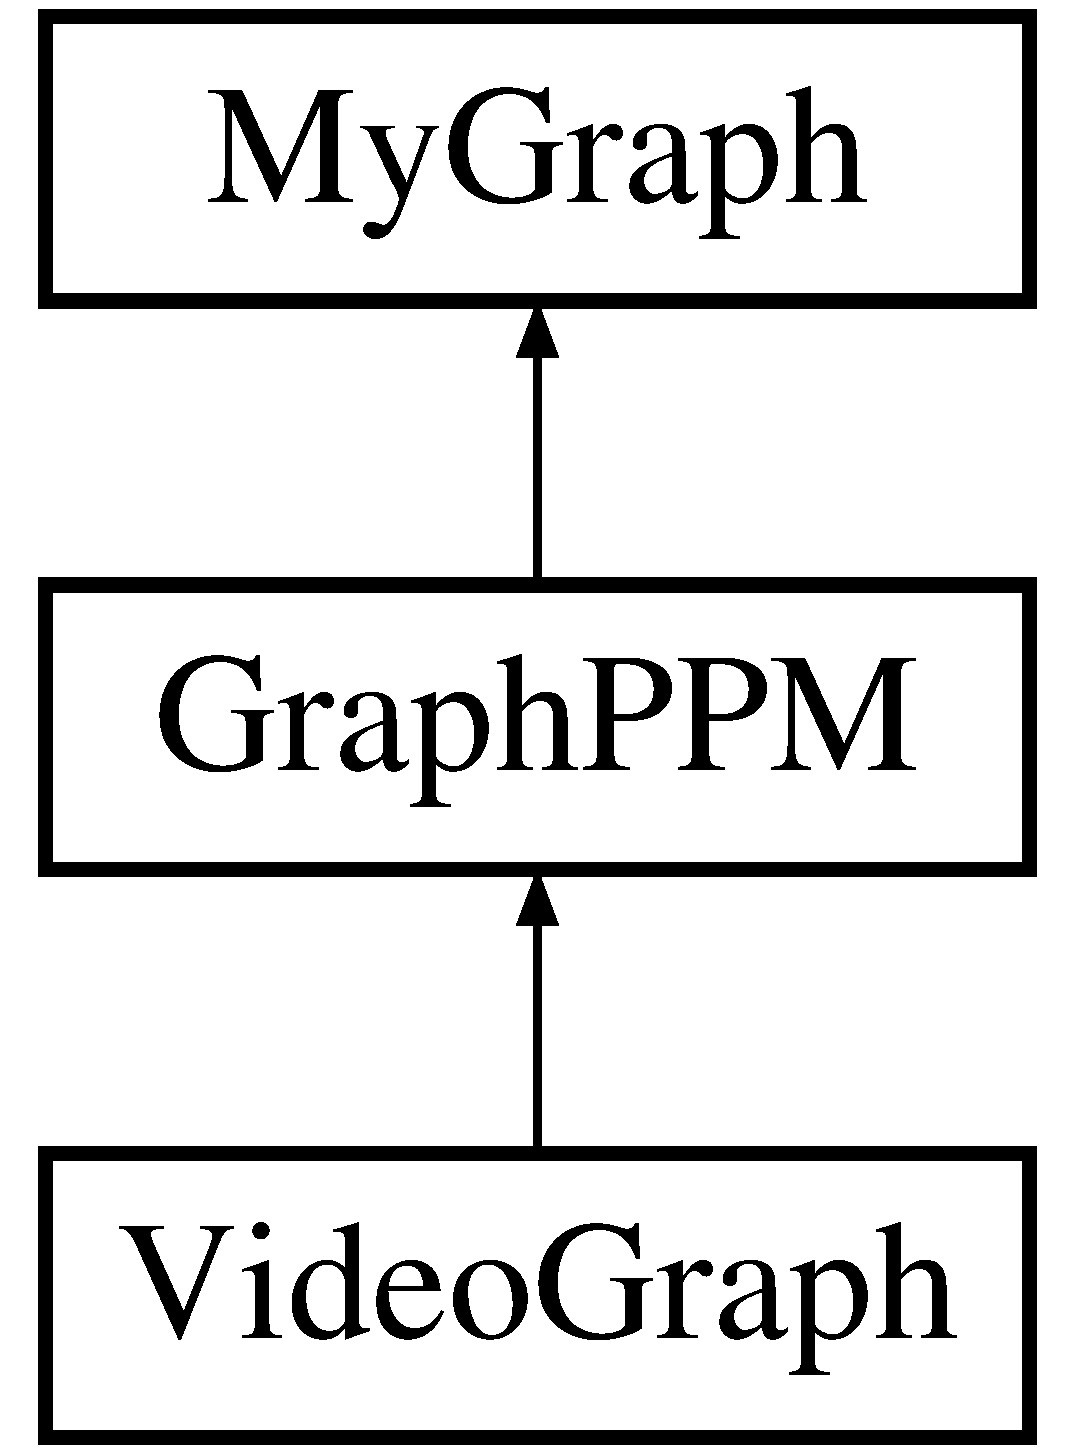
\includegraphics[height=3cm]{classVideoGraph}
\end{center}
\end{figure}
\subsection*{Public Member Functions}
\begin{CompactItemize}
\item 
{\bf BeliefPtr} {\bf getOrigBlfFromMp} (int key)
\item 
{\bf VideoNode} $\ast$ {\bf addNode} ({\bf VideoNode} $\ast$np)
\item 
map$<$ {\bf VI}, {\bf LD}, {\bf VCMP}$<$ {\bf INT} $>$ $>$ {\bf getGaussianNeighbours} ({\bf VI} v, {\bf LD} NH, {\bf LD} T)
\item 
{\bf VideoGraph} ({\bf VideoReader} $\ast$\_\-reader, bool \_\-isGray=true, int numL=4, int \_\-rx=4, int \_\-ry=4, int \_\-cx=2, int \_\-cy=2)
\item 
virtual {\bf $\sim$VideoGraph} ()
\item 
void {\bf updateCondBlfMp} (IplImage $\ast$last\_\-frame, IplImage $\ast$curr\_\-frame, IplImage $\ast$mask\_\-frame)
\item 
int {\bf addCondBlf} (vector$<$ {\bf INT} $>$ pastVals, vector$<$ {\bf INT} $>$ nextVals)
\item 
void {\bf setNodeCondBlf} ({\bf VideoNode} $\ast$vn)
\item 
void {\bf genSubRegions} ()
\begin{CompactList}\small\item\em this function adds the requisite graph structure to the \doxyref{VideoGraph}{p.}{classVideoGraph} \item\end{CompactList}\item 
vector$<$ {\bf VideoNode} $\ast$ $>$ {\bf getMaximalUnfilledRegions} ()
\item 
{\bf StatePtr} {\bf readNodeFromFrame} ({\bf VideoNode} $\ast$vn, IplImage $\ast$frame)
\begin{CompactList}\small\item\em read up the node and get equivalent state pointer \item\end{CompactList}\item 
vector$<$ pair$<$ {\bf StatePtr}, {\bf LD} $>$ $>$ {\bf getNextStateCands} ({\bf VideoNode} $\ast$vn, IplImage $\ast$frame, {\bf LD} T=0.1)
\begin{CompactList}\small\item\em ultimately has to look at gaussian mixture model of the K-NN states \item\end{CompactList}\item 
int {\bf updateNodeBlf} ({\bf VideoNode} $\ast$vn, IplImage $\ast$frame)
\item 
int {\bf updateAllNodes} (IplImage $\ast$frame, IplImage $\ast$mask\_\-frame)
\item 
void {\bf getNextFramePPM} (IplImage $\ast$frame, IplImage $\ast$holes)
\begin{CompactList}\small\item\em holes(grayscale) convention = 255 (hole) ... 0 (no hole) \item\end{CompactList}\item 
{\bf LD} {\bf getNodeMaskPct} ({\bf VideoNode} $\ast$vn, IplImage $\ast$mask\_\-frame)
\item 
void {\bf initMessages} ({\bf VideoNode} $\ast$vnp, {\bf VideoNode} $\ast$vnc, map$<$ {\bf VI}, {\bf LD}, {\bf VCMP}$<$ {\bf INT} $>$ $>$ choices)
\item 
void {\bf updateMessages} ({\bf VideoNode} $\ast$vnp, {\bf VideoNode} $\ast$vnc, map$<$ {\bf VI}, {\bf LD}, {\bf VCMP}$<$ {\bf INT} $>$ $>$ choices)
\item 
void {\bf PPM\_\-step2} (IplImage $\ast$frame, {\bf LD} candT)
\item 
bool {\bf isValid} (int x, int y, int xi=0, int yi=0, int xl=-1, int yl=-1)
\item 
bool {\bf getAbsolutePixel} (string nid, int i, int j, {\bf StatePtr} sptr, vector$<$ {\bf INT} $>$ $\ast$result)
\item 
{\bf StatePtr} {\bf getChildStatePtr} (string parId, string childId, {\bf StatePtr} parState)
\item 
void {\bf updateChildAugments} ({\bf VideoNode} $\ast$vn, {\bf StatePtr} sOld)
\item 
void {\bf updateParentAugments} ({\bf VideoNode} $\ast$vn, {\bf StatePtr} oldState)
\item 
IplImage $\ast$ {\bf inPaint} (IplImage $\ast$input\_\-frame, IplImage $\ast$mask\_\-frame)
\item 
vector$<$ pair$<$ int, int $>$ $>$ {\bf getNodeUnfilledPixels} ({\bf VideoNode} $\ast$vn, IplImage $\ast$mask\_\-frame)
\item 
bool {\bf isMaskedPixel} (int i, int j, IplImage $\ast$mask\_\-frame)
\item 
vector$<$ pair$<$ {\bf StatePtr}, {\bf LD} $>$ $>$ {\bf getMatchingStates} ({\bf VideoNode} $\ast$vn, IplImage $\ast$frame, IplImage $\ast$mask\_\-frame, bool approx=false)
\item 
void {\bf updateMaskStatus} (IplImage $\ast$mask\_\-frame)
\item 
void {\bf fillFrame0} ()
\item 
void {\bf fillFrame1} (bool lookMax=false)
\item 
bool {\bf isPartialMatch} ({\bf StatePtr} s1, {\bf StatePtr} s2, {\bf StatePtr} mask)
\item 
{\bf BeliefPtr} {\bf getApproxBlf} ({\bf VideoNode} $\ast$vn, {\bf StatePtr} sOld)
\item 
vector$<$ pair$<$ {\bf VideoNode} $\ast$, {\bf LD} $>$ $>$ {\bf getIncompleteList} (IplImage $\ast$mask\_\-frame)
\item 
bool {\bf isClose} ({\bf StatePtr} s1, {\bf StatePtr} s2, int NL, {\bf LD} distS)
\item 
vector$<$ pair$<$ {\bf StatePtr}, {\bf LD} $>$ $>$ {\bf getMaximalPixelPr} ({\bf VideoNode} $\ast$vn, int i, int j)
\item 
void {\bf clearAllNodes} ()
\item 
void {\bf clearCondBlfMp} ()
\item 
void {\bf initLocals} ()
\item 
void {\bf getCandidates} (IplImage $\ast$last\_\-frame, IplImage $\ast$input\_\-frame, IplImage $\ast$mask\_\-frame)
\item 
{\bf StatePtr} {\bf getChildStatePtr} ({\bf NodePtr} vp, {\bf NodePtr} vc, {\bf StatePtr} parState)
\end{CompactItemize}
\subsection*{Public Attributes}
\begin{CompactItemize}
\item 
IplImage $\ast$ {\bf inpainted\_\-frame}
\begin{CompactList}\small\item\em the inpainting frame \item\end{CompactList}\item 
IplImage $\ast$ {\bf local\_\-mask}
\item 
IplImage $\ast$ {\bf output\_\-frame}
\begin{CompactList}\small\item\em pointer to reader output frame \item\end{CompactList}\item 
IplImage $\ast$ {\bf true\_\-frame}
\begin{CompactList}\small\item\em pointer to the reader true frame \item\end{CompactList}\end{CompactItemize}
\subsection*{Private Member Functions}
\begin{CompactItemize}
\item 
pair$<$ {\bf StatePtr}, {\bf LD} $>$ {\bf getBestState0} ({\bf VideoNode} $\ast$vn)
\end{CompactItemize}
\subsection*{Private Attributes}
\begin{CompactItemize}
\item 
map$<$ int, {\bf ConditionalBelief} $\ast$ $>$ {\bf blfMp}
\begin{CompactList}\small\item\em the belief maps for number of variables under question \item\end{CompactList}\item 
map$<$ int, {\bf BeliefPtr} $>$ {\bf pOrigMp}
\begin{CompactList}\small\item\em the belief maps for bOrig \item\end{CompactList}\item 
int {\bf numLvls}
\begin{CompactList}\small\item\em the levels \item\end{CompactList}\item 
bool {\bf isGray}
\begin{CompactList}\small\item\em whether is gray or not \item\end{CompactList}\item 
vector$<$ int $>$ {\bf levels}
\begin{CompactList}\small\item\em the levels that will be present in the video (0..255) \item\end{CompactList}\item 
{\bf VideoReader} $\ast$ {\bf reader}
\begin{CompactList}\small\item\em the reader \item\end{CompactList}\item 
int {\bf rx}
\begin{CompactList}\small\item\em biggest region width \item\end{CompactList}\item 
int {\bf ry}
\begin{CompactList}\small\item\em biggest region size \item\end{CompactList}\item 
int {\bf cx}
\begin{CompactList}\small\item\em how much x-overlap between current and next region \item\end{CompactList}\item 
int {\bf cy}
\begin{CompactList}\small\item\em how much y-overlap between current and next region \item\end{CompactList}\item 
int {\bf N1}
\begin{CompactList}\small\item\em how many rows \item\end{CompactList}\item 
int {\bf N2}
\begin{CompactList}\small\item\em how many columns \item\end{CompactList}\item 
int {\bf hits}
\begin{CompactList}\small\item\em the number of cond beliefs that have been duplicated \item\end{CompactList}\item 
int {\bf misses}
\begin{CompactList}\small\item\em the number of frames that have been missed \item\end{CompactList}\item 
{\bf LD} {\bf sigma}
\begin{CompactList}\small\item\em the sigma value for gaussian around the mean value \item\end{CompactList}\item 
{\bf LD} {\bf nearestT}
\item 
{\bf LD} {\bf selectThreshold}
\begin{CompactList}\small\item\em the threshold for max-probability \item\end{CompactList}\item 
int {\bf parAugmentNotFound}
\item 
int {\bf parAugmentFound}
\end{CompactItemize}


\subsection{Constructor \& Destructor Documentation}
\index{VideoGraph@{VideoGraph}!VideoGraph@{VideoGraph}}
\index{VideoGraph@{VideoGraph}!VideoGraph@{VideoGraph}}
\subsubsection{\setlength{\rightskip}{0pt plus 5cm}VideoGraph::VideoGraph ({\bf VideoReader} $\ast$ {\em \_\-reader}, bool {\em \_\-isGray} = {\tt true}, int {\em numL} = {\tt 4}, int {\em \_\-rx} = {\tt 4}, int {\em \_\-ry} = {\tt 4}, int {\em \_\-cx} = {\tt 2}, int {\em \_\-cy} = {\tt 2})}\label{classVideoGraph_c71e577507f20c12ea997c947fb172a0}


\index{VideoGraph@{VideoGraph}!~VideoGraph@{$\sim$VideoGraph}}
\index{~VideoGraph@{$\sim$VideoGraph}!VideoGraph@{VideoGraph}}
\subsubsection{\setlength{\rightskip}{0pt plus 5cm}VideoGraph::$\sim$VideoGraph ()\hspace{0.3cm}{\tt  [virtual]}}\label{classVideoGraph_d70ffc6a39c30301c8091bda6cafa293}




\subsection{Member Function Documentation}
\index{VideoGraph@{VideoGraph}!getBestState0@{getBestState0}}
\index{getBestState0@{getBestState0}!VideoGraph@{VideoGraph}}
\subsubsection{\setlength{\rightskip}{0pt plus 5cm}pair$<$ {\bf StatePtr}, {\bf LD} $>$ VideoGraph::getBestState0 ({\bf VideoNode} $\ast$ {\em vn})\hspace{0.3cm}{\tt  [private]}}\label{classVideoGraph_9531cdfa7ef234edbe14b61a8cfd09a0}


\index{VideoGraph@{VideoGraph}!getOrigBlfFromMp@{getOrigBlfFromMp}}
\index{getOrigBlfFromMp@{getOrigBlfFromMp}!VideoGraph@{VideoGraph}}
\subsubsection{\setlength{\rightskip}{0pt plus 5cm}{\bf BeliefPtr} VideoGraph::getOrigBlfFromMp (int {\em key})\hspace{0.3cm}{\tt  [inline]}}\label{classVideoGraph_1752f6d20f74a0b1d05dc16a9c30c0fa}


\index{VideoGraph@{VideoGraph}!addNode@{addNode}}
\index{addNode@{addNode}!VideoGraph@{VideoGraph}}
\subsubsection{\setlength{\rightskip}{0pt plus 5cm}{\bf VideoNode}$\ast$ VideoGraph::addNode ({\bf VideoNode} $\ast$ {\em np})\hspace{0.3cm}{\tt  [inline]}}\label{classVideoGraph_309cbe38154dffdacad5fa8fa24c8369}


\index{VideoGraph@{VideoGraph}!getGaussianNeighbours@{getGaussianNeighbours}}
\index{getGaussianNeighbours@{getGaussianNeighbours}!VideoGraph@{VideoGraph}}
\subsubsection{\setlength{\rightskip}{0pt plus 5cm}map$<${\bf VI}, {\bf LD}, {\bf VCMP}$<${\bf INT}$>$ $>$ VideoGraph::getGaussianNeighbours ({\bf VI} {\em v}, {\bf LD} {\em NH}, {\bf LD} {\em T})}\label{classVideoGraph_d0c335f75e0460809a78fa356a5f45c1}


\index{VideoGraph@{VideoGraph}!updateCondBlfMp@{updateCondBlfMp}}
\index{updateCondBlfMp@{updateCondBlfMp}!VideoGraph@{VideoGraph}}
\subsubsection{\setlength{\rightskip}{0pt plus 5cm}void VideoGraph::updateCondBlfMp (IplImage $\ast$ {\em last\_\-frame}, IplImage $\ast$ {\em curr\_\-frame}, IplImage $\ast$ {\em mask\_\-frame})}\label{classVideoGraph_b0aa9baed334fae1d815a18b2ed528bb}


\index{VideoGraph@{VideoGraph}!addCondBlf@{addCondBlf}}
\index{addCondBlf@{addCondBlf}!VideoGraph@{VideoGraph}}
\subsubsection{\setlength{\rightskip}{0pt plus 5cm}int VideoGraph::addCondBlf (vector$<$ {\bf INT} $>$ {\em pastVals}, vector$<$ {\bf INT} $>$ {\em nextVals})}\label{classVideoGraph_eb9575760cf698e05928b7245f294f9d}


\index{VideoGraph@{VideoGraph}!setNodeCondBlf@{setNodeCondBlf}}
\index{setNodeCondBlf@{setNodeCondBlf}!VideoGraph@{VideoGraph}}
\subsubsection{\setlength{\rightskip}{0pt plus 5cm}void VideoGraph::setNodeCondBlf ({\bf VideoNode} $\ast$ {\em vn})}\label{classVideoGraph_c6e953524c70a19f8808b0c7d284e165}


\index{VideoGraph@{VideoGraph}!genSubRegions@{genSubRegions}}
\index{genSubRegions@{genSubRegions}!VideoGraph@{VideoGraph}}
\subsubsection{\setlength{\rightskip}{0pt plus 5cm}void VideoGraph::genSubRegions ()}\label{classVideoGraph_af45bb4776b8c55d5110d40624f3ffce}


this function adds the requisite graph structure to the \doxyref{VideoGraph}{p.}{classVideoGraph} 

\index{VideoGraph@{VideoGraph}!getMaximalUnfilledRegions@{getMaximalUnfilledRegions}}
\index{getMaximalUnfilledRegions@{getMaximalUnfilledRegions}!VideoGraph@{VideoGraph}}
\subsubsection{\setlength{\rightskip}{0pt plus 5cm}vector$<${\bf VideoNode}$\ast$$>$ VideoGraph::getMaximalUnfilledRegions ()}\label{classVideoGraph_ec510cbdf647928a51397984f899351d}


\index{VideoGraph@{VideoGraph}!readNodeFromFrame@{readNodeFromFrame}}
\index{readNodeFromFrame@{readNodeFromFrame}!VideoGraph@{VideoGraph}}
\subsubsection{\setlength{\rightskip}{0pt plus 5cm}{\bf StatePtr} VideoGraph::readNodeFromFrame ({\bf VideoNode} $\ast$ {\em vn}, IplImage $\ast$ {\em frame})}\label{classVideoGraph_8e23915b2b4060749f09bfb0784f4777}


read up the node and get equivalent state pointer 

\index{VideoGraph@{VideoGraph}!getNextStateCands@{getNextStateCands}}
\index{getNextStateCands@{getNextStateCands}!VideoGraph@{VideoGraph}}
\subsubsection{\setlength{\rightskip}{0pt plus 5cm}vector$<$ pair$<$ {\bf StatePtr}, {\bf LD} $>$ $>$ VideoGraph::getNextStateCands ({\bf VideoNode} $\ast$ {\em vn}, IplImage $\ast$ {\em frame}, {\bf LD} {\em T} = {\tt 0.1})}\label{classVideoGraph_d23ce958583f4d6e67caf2af67cbd1ec}


ultimately has to look at gaussian mixture model of the K-NN states 

\index{VideoGraph@{VideoGraph}!updateNodeBlf@{updateNodeBlf}}
\index{updateNodeBlf@{updateNodeBlf}!VideoGraph@{VideoGraph}}
\subsubsection{\setlength{\rightskip}{0pt plus 5cm}int VideoGraph::updateNodeBlf ({\bf VideoNode} $\ast$ {\em vn}, IplImage $\ast$ {\em frame})}\label{classVideoGraph_e3600547c757a8855db8d8deccce65ce}


\index{VideoGraph@{VideoGraph}!updateAllNodes@{updateAllNodes}}
\index{updateAllNodes@{updateAllNodes}!VideoGraph@{VideoGraph}}
\subsubsection{\setlength{\rightskip}{0pt plus 5cm}int VideoGraph::updateAllNodes (IplImage $\ast$ {\em frame}, IplImage $\ast$ {\em mask\_\-frame})}\label{classVideoGraph_e1e4fce017fd2437d0f9da0b852965ee}


\index{VideoGraph@{VideoGraph}!getNextFramePPM@{getNextFramePPM}}
\index{getNextFramePPM@{getNextFramePPM}!VideoGraph@{VideoGraph}}
\subsubsection{\setlength{\rightskip}{0pt plus 5cm}void VideoGraph::getNextFramePPM (IplImage $\ast$ {\em frame}, IplImage $\ast$ {\em holes})}\label{classVideoGraph_ae5639a15ce8bdc7cc59f084d8709414}


holes(grayscale) convention = 255 (hole) ... 0 (no hole) 

\index{VideoGraph@{VideoGraph}!getNodeMaskPct@{getNodeMaskPct}}
\index{getNodeMaskPct@{getNodeMaskPct}!VideoGraph@{VideoGraph}}
\subsubsection{\setlength{\rightskip}{0pt plus 5cm}{\bf LD} VideoGraph::getNodeMaskPct ({\bf VideoNode} $\ast$ {\em vn}, IplImage $\ast$ {\em mask\_\-frame})}\label{classVideoGraph_88d5e9d8cc881f0095d4b8cbf6b2d661}


\index{VideoGraph@{VideoGraph}!initMessages@{initMessages}}
\index{initMessages@{initMessages}!VideoGraph@{VideoGraph}}
\subsubsection{\setlength{\rightskip}{0pt plus 5cm}void VideoGraph::initMessages ({\bf VideoNode} $\ast$ {\em vnp}, {\bf VideoNode} $\ast$ {\em vnc}, map$<$ {\bf VI}, {\bf LD}, {\bf VCMP}$<$ {\bf INT} $>$ $>$ {\em choices})}\label{classVideoGraph_dea952dbc2d364b64ebf8a8dc7509eb5}


\index{VideoGraph@{VideoGraph}!updateMessages@{updateMessages}}
\index{updateMessages@{updateMessages}!VideoGraph@{VideoGraph}}
\subsubsection{\setlength{\rightskip}{0pt plus 5cm}void VideoGraph::updateMessages ({\bf VideoNode} $\ast$ {\em vnp}, {\bf VideoNode} $\ast$ {\em vnc}, map$<$ {\bf VI}, {\bf LD}, {\bf VCMP}$<$ {\bf INT} $>$ $>$ {\em choices})}\label{classVideoGraph_6f0480f5aff68515ba810aa20119aa39}


\index{VideoGraph@{VideoGraph}!PPM_step2@{PPM\_\-step2}}
\index{PPM_step2@{PPM\_\-step2}!VideoGraph@{VideoGraph}}
\subsubsection{\setlength{\rightskip}{0pt plus 5cm}void VideoGraph::PPM\_\-step2 (IplImage $\ast$ {\em frame}, {\bf LD} {\em candT})}\label{classVideoGraph_3f59d46d63f993de3f8e17a1a7479f0d}


\index{VideoGraph@{VideoGraph}!isValid@{isValid}}
\index{isValid@{isValid}!VideoGraph@{VideoGraph}}
\subsubsection{\setlength{\rightskip}{0pt plus 5cm}bool VideoGraph::isValid (int {\em x}, int {\em y}, int {\em xi} = {\tt 0}, int {\em yi} = {\tt 0}, int {\em xl} = {\tt -1}, int {\em yl} = {\tt -1})}\label{classVideoGraph_ed75bcece886e9523b75933da823784a}


\index{VideoGraph@{VideoGraph}!getAbsolutePixel@{getAbsolutePixel}}
\index{getAbsolutePixel@{getAbsolutePixel}!VideoGraph@{VideoGraph}}
\subsubsection{\setlength{\rightskip}{0pt plus 5cm}bool VideoGraph::getAbsolutePixel (string {\em nid}, int {\em i}, int {\em j}, {\bf StatePtr} {\em sptr}, vector$<$ {\bf INT} $>$ $\ast$ {\em result})}\label{classVideoGraph_5a0e5265411b87ae2217972c4db5c0cb}


\index{VideoGraph@{VideoGraph}!getChildStatePtr@{getChildStatePtr}}
\index{getChildStatePtr@{getChildStatePtr}!VideoGraph@{VideoGraph}}
\subsubsection{\setlength{\rightskip}{0pt plus 5cm}{\bf StatePtr} VideoGraph::getChildStatePtr (string {\em parId}, string {\em childId}, {\bf StatePtr} {\em parState})}\label{classVideoGraph_ca9ae8e0d5a27cbf4598c60799c04081}


\index{VideoGraph@{VideoGraph}!updateChildAugments@{updateChildAugments}}
\index{updateChildAugments@{updateChildAugments}!VideoGraph@{VideoGraph}}
\subsubsection{\setlength{\rightskip}{0pt plus 5cm}void VideoGraph::updateChildAugments ({\bf VideoNode} $\ast$ {\em vn}, {\bf StatePtr} {\em sOld})}\label{classVideoGraph_f97ae97bea7bcc80523d5144e62be37b}


\index{VideoGraph@{VideoGraph}!updateParentAugments@{updateParentAugments}}
\index{updateParentAugments@{updateParentAugments}!VideoGraph@{VideoGraph}}
\subsubsection{\setlength{\rightskip}{0pt plus 5cm}void VideoGraph::updateParentAugments ({\bf VideoNode} $\ast$ {\em vn}, {\bf StatePtr} {\em oldState})}\label{classVideoGraph_2da7bbfb7037dcb4cb77ddbf512be38f}


\index{VideoGraph@{VideoGraph}!inPaint@{inPaint}}
\index{inPaint@{inPaint}!VideoGraph@{VideoGraph}}
\subsubsection{\setlength{\rightskip}{0pt plus 5cm}IplImage $\ast$ VideoGraph::inPaint (IplImage $\ast$ {\em input\_\-frame}, IplImage $\ast$ {\em mask\_\-frame})}\label{classVideoGraph_288c0f0e3cc4bd415b4be7805c71b414}


\index{VideoGraph@{VideoGraph}!getNodeUnfilledPixels@{getNodeUnfilledPixels}}
\index{getNodeUnfilledPixels@{getNodeUnfilledPixels}!VideoGraph@{VideoGraph}}
\subsubsection{\setlength{\rightskip}{0pt plus 5cm}vector$<$ pair$<$ int, int $>$ $>$ VideoGraph::getNodeUnfilledPixels ({\bf VideoNode} $\ast$ {\em vn}, IplImage $\ast$ {\em mask\_\-frame})}\label{classVideoGraph_9022e09e81c10e1a5fbb4347a9428470}


\index{VideoGraph@{VideoGraph}!isMaskedPixel@{isMaskedPixel}}
\index{isMaskedPixel@{isMaskedPixel}!VideoGraph@{VideoGraph}}
\subsubsection{\setlength{\rightskip}{0pt plus 5cm}bool VideoGraph::isMaskedPixel (int {\em i}, int {\em j}, IplImage $\ast$ {\em mask\_\-frame})}\label{classVideoGraph_2dc39de1bc815856e0beed4f2e9d8081}


\index{VideoGraph@{VideoGraph}!getMatchingStates@{getMatchingStates}}
\index{getMatchingStates@{getMatchingStates}!VideoGraph@{VideoGraph}}
\subsubsection{\setlength{\rightskip}{0pt plus 5cm}vector$<$ pair$<$ {\bf StatePtr}, {\bf LD} $>$ $>$ VideoGraph::getMatchingStates ({\bf VideoNode} $\ast$ {\em vn}, IplImage $\ast$ {\em frame}, IplImage $\ast$ {\em mask\_\-frame}, bool {\em approx} = {\tt false})}\label{classVideoGraph_73caa2bebc4e83e3da0011a822ece849}


\index{VideoGraph@{VideoGraph}!updateMaskStatus@{updateMaskStatus}}
\index{updateMaskStatus@{updateMaskStatus}!VideoGraph@{VideoGraph}}
\subsubsection{\setlength{\rightskip}{0pt plus 5cm}void VideoGraph::updateMaskStatus (IplImage $\ast$ {\em mask\_\-frame})}\label{classVideoGraph_29b757cf3a1454e4348e729778c6735f}


\index{VideoGraph@{VideoGraph}!fillFrame0@{fillFrame0}}
\index{fillFrame0@{fillFrame0}!VideoGraph@{VideoGraph}}
\subsubsection{\setlength{\rightskip}{0pt plus 5cm}void VideoGraph::fillFrame0 ()}\label{classVideoGraph_f179c4fcc35c635738cfef0082a869a1}


\index{VideoGraph@{VideoGraph}!fillFrame1@{fillFrame1}}
\index{fillFrame1@{fillFrame1}!VideoGraph@{VideoGraph}}
\subsubsection{\setlength{\rightskip}{0pt plus 5cm}void VideoGraph::fillFrame1 (bool {\em lookMax} = {\tt false})}\label{classVideoGraph_029b777f551318e3f070c519ce814715}


\index{VideoGraph@{VideoGraph}!isPartialMatch@{isPartialMatch}}
\index{isPartialMatch@{isPartialMatch}!VideoGraph@{VideoGraph}}
\subsubsection{\setlength{\rightskip}{0pt plus 5cm}bool VideoGraph::isPartialMatch ({\bf StatePtr} {\em s1}, {\bf StatePtr} {\em s2}, {\bf StatePtr} {\em mask})}\label{classVideoGraph_6557d18e0d607e426d634f9c5ef5e464}


\index{VideoGraph@{VideoGraph}!getApproxBlf@{getApproxBlf}}
\index{getApproxBlf@{getApproxBlf}!VideoGraph@{VideoGraph}}
\subsubsection{\setlength{\rightskip}{0pt plus 5cm}{\bf BeliefPtr} VideoGraph::getApproxBlf ({\bf VideoNode} $\ast$ {\em vn}, {\bf StatePtr} {\em sOld})}\label{classVideoGraph_6925027f23efb0021fe93bbb1a7b3d23}


\index{VideoGraph@{VideoGraph}!getIncompleteList@{getIncompleteList}}
\index{getIncompleteList@{getIncompleteList}!VideoGraph@{VideoGraph}}
\subsubsection{\setlength{\rightskip}{0pt plus 5cm}vector$<$ pair$<$ {\bf VideoNode} $\ast$, {\bf LD} $>$ $>$ VideoGraph::getIncompleteList (IplImage $\ast$ {\em mask\_\-frame})}\label{classVideoGraph_9a0548bc4181b53fa00b48bb3c671445}


\index{VideoGraph@{VideoGraph}!isClose@{isClose}}
\index{isClose@{isClose}!VideoGraph@{VideoGraph}}
\subsubsection{\setlength{\rightskip}{0pt plus 5cm}bool VideoGraph::isClose ({\bf StatePtr} {\em s1}, {\bf StatePtr} {\em s2}, int {\em NL}, {\bf LD} {\em distS})}\label{classVideoGraph_d09a5dbc367d381dc75a979082852156}


\index{VideoGraph@{VideoGraph}!getMaximalPixelPr@{getMaximalPixelPr}}
\index{getMaximalPixelPr@{getMaximalPixelPr}!VideoGraph@{VideoGraph}}
\subsubsection{\setlength{\rightskip}{0pt plus 5cm}vector$<$ pair$<$ {\bf StatePtr}, {\bf LD} $>$ $>$ VideoGraph::getMaximalPixelPr ({\bf VideoNode} $\ast$ {\em vn}, int {\em i}, int {\em j})}\label{classVideoGraph_da8ec222464e68881ada2e4a62c2a72b}


\index{VideoGraph@{VideoGraph}!clearAllNodes@{clearAllNodes}}
\index{clearAllNodes@{clearAllNodes}!VideoGraph@{VideoGraph}}
\subsubsection{\setlength{\rightskip}{0pt plus 5cm}void VideoGraph::clearAllNodes ()}\label{classVideoGraph_fbc9fe10a385560c993d81bb7fe9ac33}


\index{VideoGraph@{VideoGraph}!clearCondBlfMp@{clearCondBlfMp}}
\index{clearCondBlfMp@{clearCondBlfMp}!VideoGraph@{VideoGraph}}
\subsubsection{\setlength{\rightskip}{0pt plus 5cm}void VideoGraph::clearCondBlfMp ()}\label{classVideoGraph_64fe11928c7c207c9d552eae790cf6b9}


\index{VideoGraph@{VideoGraph}!initLocals@{initLocals}}
\index{initLocals@{initLocals}!VideoGraph@{VideoGraph}}
\subsubsection{\setlength{\rightskip}{0pt plus 5cm}void VideoGraph::initLocals ()}\label{classVideoGraph_cd2142a933ab36b5355a5ba409442e3c}


\index{VideoGraph@{VideoGraph}!getCandidates@{getCandidates}}
\index{getCandidates@{getCandidates}!VideoGraph@{VideoGraph}}
\subsubsection{\setlength{\rightskip}{0pt plus 5cm}void VideoGraph::getCandidates (IplImage $\ast$ {\em last\_\-frame}, IplImage $\ast$ {\em input\_\-frame}, IplImage $\ast$ {\em mask\_\-frame})}\label{classVideoGraph_0cc989668c7c1881ab89c63117621657}


\index{VideoGraph@{VideoGraph}!getChildStatePtr@{getChildStatePtr}}
\index{getChildStatePtr@{getChildStatePtr}!VideoGraph@{VideoGraph}}
\subsubsection{\setlength{\rightskip}{0pt plus 5cm}{\bf StatePtr} VideoGraph::getChildStatePtr ({\bf NodePtr} {\em vp}, {\bf NodePtr} {\em vc}, {\bf StatePtr} {\em parState})\hspace{0.3cm}{\tt  [inline, virtual]}}\label{classVideoGraph_9e6275280e01ab9b37b52e7cf92ddd2d}




Implements {\bf GraphPPM} \doxyref{}{p.}{classGraphPPM_b245aae058d0b252df985651c8fcc2eb}.

\subsection{Member Data Documentation}
\index{VideoGraph@{VideoGraph}!blfMp@{blfMp}}
\index{blfMp@{blfMp}!VideoGraph@{VideoGraph}}
\subsubsection{\setlength{\rightskip}{0pt plus 5cm}map$<$int, {\bf ConditionalBelief}$\ast$ $>$ {\bf VideoGraph::blfMp}\hspace{0.3cm}{\tt  [private]}}\label{classVideoGraph_3a7eb105eb81b07f72042a34df9b6aad}


the belief maps for number of variables under question 

\index{VideoGraph@{VideoGraph}!pOrigMp@{pOrigMp}}
\index{pOrigMp@{pOrigMp}!VideoGraph@{VideoGraph}}
\subsubsection{\setlength{\rightskip}{0pt plus 5cm}map$<$int, {\bf BeliefPtr}$>$ {\bf VideoGraph::pOrigMp}\hspace{0.3cm}{\tt  [private]}}\label{classVideoGraph_392f6c68aa8ea5ceb2349a93241d550b}


the belief maps for bOrig 

\index{VideoGraph@{VideoGraph}!numLvls@{numLvls}}
\index{numLvls@{numLvls}!VideoGraph@{VideoGraph}}
\subsubsection{\setlength{\rightskip}{0pt plus 5cm}int {\bf VideoGraph::numLvls}\hspace{0.3cm}{\tt  [private]}}\label{classVideoGraph_96f834448fa5cf950840d66c41e9cdec}


the levels 

\index{VideoGraph@{VideoGraph}!isGray@{isGray}}
\index{isGray@{isGray}!VideoGraph@{VideoGraph}}
\subsubsection{\setlength{\rightskip}{0pt plus 5cm}bool {\bf VideoGraph::isGray}\hspace{0.3cm}{\tt  [private]}}\label{classVideoGraph_92f68a8f0b1177cae199eeb72e54f6b5}


whether is gray or not 

\index{VideoGraph@{VideoGraph}!levels@{levels}}
\index{levels@{levels}!VideoGraph@{VideoGraph}}
\subsubsection{\setlength{\rightskip}{0pt plus 5cm}vector$<$int$>$ {\bf VideoGraph::levels}\hspace{0.3cm}{\tt  [private]}}\label{classVideoGraph_9488fbaa66e4a81e7612ebd795efe64f}


the levels that will be present in the video (0..255) 

\index{VideoGraph@{VideoGraph}!reader@{reader}}
\index{reader@{reader}!VideoGraph@{VideoGraph}}
\subsubsection{\setlength{\rightskip}{0pt plus 5cm}{\bf VideoReader}$\ast$ {\bf VideoGraph::reader}\hspace{0.3cm}{\tt  [private]}}\label{classVideoGraph_2028023e314c8267759fb62ec448aecc}


the reader 

\index{VideoGraph@{VideoGraph}!rx@{rx}}
\index{rx@{rx}!VideoGraph@{VideoGraph}}
\subsubsection{\setlength{\rightskip}{0pt plus 5cm}int {\bf VideoGraph::rx}\hspace{0.3cm}{\tt  [private]}}\label{classVideoGraph_0a429d2da38708c8fac0077d76718816}


biggest region width 

\index{VideoGraph@{VideoGraph}!ry@{ry}}
\index{ry@{ry}!VideoGraph@{VideoGraph}}
\subsubsection{\setlength{\rightskip}{0pt plus 5cm}int {\bf VideoGraph::ry}\hspace{0.3cm}{\tt  [private]}}\label{classVideoGraph_d6f12308b98c416ffca99c98bc872cb0}


biggest region size 

\index{VideoGraph@{VideoGraph}!cx@{cx}}
\index{cx@{cx}!VideoGraph@{VideoGraph}}
\subsubsection{\setlength{\rightskip}{0pt plus 5cm}int {\bf VideoGraph::cx}\hspace{0.3cm}{\tt  [private]}}\label{classVideoGraph_fb26fafe304c8b01c866dbb2c352a36b}


how much x-overlap between current and next region 

\index{VideoGraph@{VideoGraph}!cy@{cy}}
\index{cy@{cy}!VideoGraph@{VideoGraph}}
\subsubsection{\setlength{\rightskip}{0pt plus 5cm}int {\bf VideoGraph::cy}\hspace{0.3cm}{\tt  [private]}}\label{classVideoGraph_23bf3294f2f920882fec4674718f1f0c}


how much y-overlap between current and next region 

\index{VideoGraph@{VideoGraph}!N1@{N1}}
\index{N1@{N1}!VideoGraph@{VideoGraph}}
\subsubsection{\setlength{\rightskip}{0pt plus 5cm}int {\bf VideoGraph::N1}\hspace{0.3cm}{\tt  [private]}}\label{classVideoGraph_05dd3abfee9967043420aaaff3fce547}


how many rows 

\index{VideoGraph@{VideoGraph}!N2@{N2}}
\index{N2@{N2}!VideoGraph@{VideoGraph}}
\subsubsection{\setlength{\rightskip}{0pt plus 5cm}int {\bf VideoGraph::N2}\hspace{0.3cm}{\tt  [private]}}\label{classVideoGraph_f60f4e2612cc444c8f18030af71dbbc9}


how many columns 

\index{VideoGraph@{VideoGraph}!hits@{hits}}
\index{hits@{hits}!VideoGraph@{VideoGraph}}
\subsubsection{\setlength{\rightskip}{0pt plus 5cm}int {\bf VideoGraph::hits}\hspace{0.3cm}{\tt  [private]}}\label{classVideoGraph_82583b12938e2ef4db4e5cae7a01d856}


the number of cond beliefs that have been duplicated 

\index{VideoGraph@{VideoGraph}!misses@{misses}}
\index{misses@{misses}!VideoGraph@{VideoGraph}}
\subsubsection{\setlength{\rightskip}{0pt plus 5cm}int {\bf VideoGraph::misses}\hspace{0.3cm}{\tt  [private]}}\label{classVideoGraph_de1225cdd9a602dd2e6a726e41e3e965}


the number of frames that have been missed 

\index{VideoGraph@{VideoGraph}!sigma@{sigma}}
\index{sigma@{sigma}!VideoGraph@{VideoGraph}}
\subsubsection{\setlength{\rightskip}{0pt plus 5cm}{\bf LD} {\bf VideoGraph::sigma}\hspace{0.3cm}{\tt  [private]}}\label{classVideoGraph_749c81259aa9c59e85e6e448b1a46dc5}


the sigma value for gaussian around the mean value 

\index{VideoGraph@{VideoGraph}!nearestT@{nearestT}}
\index{nearestT@{nearestT}!VideoGraph@{VideoGraph}}
\subsubsection{\setlength{\rightskip}{0pt plus 5cm}{\bf LD} {\bf VideoGraph::nearestT}\hspace{0.3cm}{\tt  [private]}}\label{classVideoGraph_9893c4483dde840e840da0f88ca21ff1}


\index{VideoGraph@{VideoGraph}!selectThreshold@{selectThreshold}}
\index{selectThreshold@{selectThreshold}!VideoGraph@{VideoGraph}}
\subsubsection{\setlength{\rightskip}{0pt plus 5cm}{\bf LD} {\bf VideoGraph::selectThreshold}\hspace{0.3cm}{\tt  [private]}}\label{classVideoGraph_69059a692b67900f619686b4f48a06f2}


the threshold for max-probability 

\index{VideoGraph@{VideoGraph}!parAugmentNotFound@{parAugmentNotFound}}
\index{parAugmentNotFound@{parAugmentNotFound}!VideoGraph@{VideoGraph}}
\subsubsection{\setlength{\rightskip}{0pt plus 5cm}int {\bf VideoGraph::parAugmentNotFound}\hspace{0.3cm}{\tt  [private]}}\label{classVideoGraph_2f5ae2f9001ec5bbec9c4d997a58cd8a}


\index{VideoGraph@{VideoGraph}!parAugmentFound@{parAugmentFound}}
\index{parAugmentFound@{parAugmentFound}!VideoGraph@{VideoGraph}}
\subsubsection{\setlength{\rightskip}{0pt plus 5cm}int {\bf VideoGraph::parAugmentFound}\hspace{0.3cm}{\tt  [private]}}\label{classVideoGraph_4879c10a87795020cc9175cd276a0d57}


\index{VideoGraph@{VideoGraph}!inpainted_frame@{inpainted\_\-frame}}
\index{inpainted_frame@{inpainted\_\-frame}!VideoGraph@{VideoGraph}}
\subsubsection{\setlength{\rightskip}{0pt plus 5cm}IplImage$\ast$ {\bf VideoGraph::inpainted\_\-frame}}\label{classVideoGraph_9338e96b5267f18ce4291a5af5e8f5f1}


the inpainting frame 

\index{VideoGraph@{VideoGraph}!local_mask@{local\_\-mask}}
\index{local_mask@{local\_\-mask}!VideoGraph@{VideoGraph}}
\subsubsection{\setlength{\rightskip}{0pt plus 5cm}IplImage$\ast$ {\bf VideoGraph::local\_\-mask}}\label{classVideoGraph_abfbba16f9b2f4940abf173ea4ab9f37}


\index{VideoGraph@{VideoGraph}!output_frame@{output\_\-frame}}
\index{output_frame@{output\_\-frame}!VideoGraph@{VideoGraph}}
\subsubsection{\setlength{\rightskip}{0pt plus 5cm}IplImage$\ast$ {\bf VideoGraph::output\_\-frame}}\label{classVideoGraph_708f6ff2e27c5c7a682a58a3deb6d7ae}


pointer to reader output frame 

\index{VideoGraph@{VideoGraph}!true_frame@{true\_\-frame}}
\index{true_frame@{true\_\-frame}!VideoGraph@{VideoGraph}}
\subsubsection{\setlength{\rightskip}{0pt plus 5cm}IplImage$\ast$ {\bf VideoGraph::true\_\-frame}}\label{classVideoGraph_c313b092ed19b2673b48dfb0e5fe5cca}


pointer to the reader true frame 



The documentation for this class was generated from the following files:\begin{CompactItemize}
\item 
inc/{\bf VideoGraph.h}\item 
src/{\bf VideoGraph.cpp}\end{CompactItemize}

\section{VideoNode Class Reference}
\label{classVideoNode}\index{VideoNode@{VideoNode}}
{\tt \#include $<$VideoNode.h$>$}

Inheritance diagram for VideoNode::\begin{figure}[H]
\begin{center}
\leavevmode
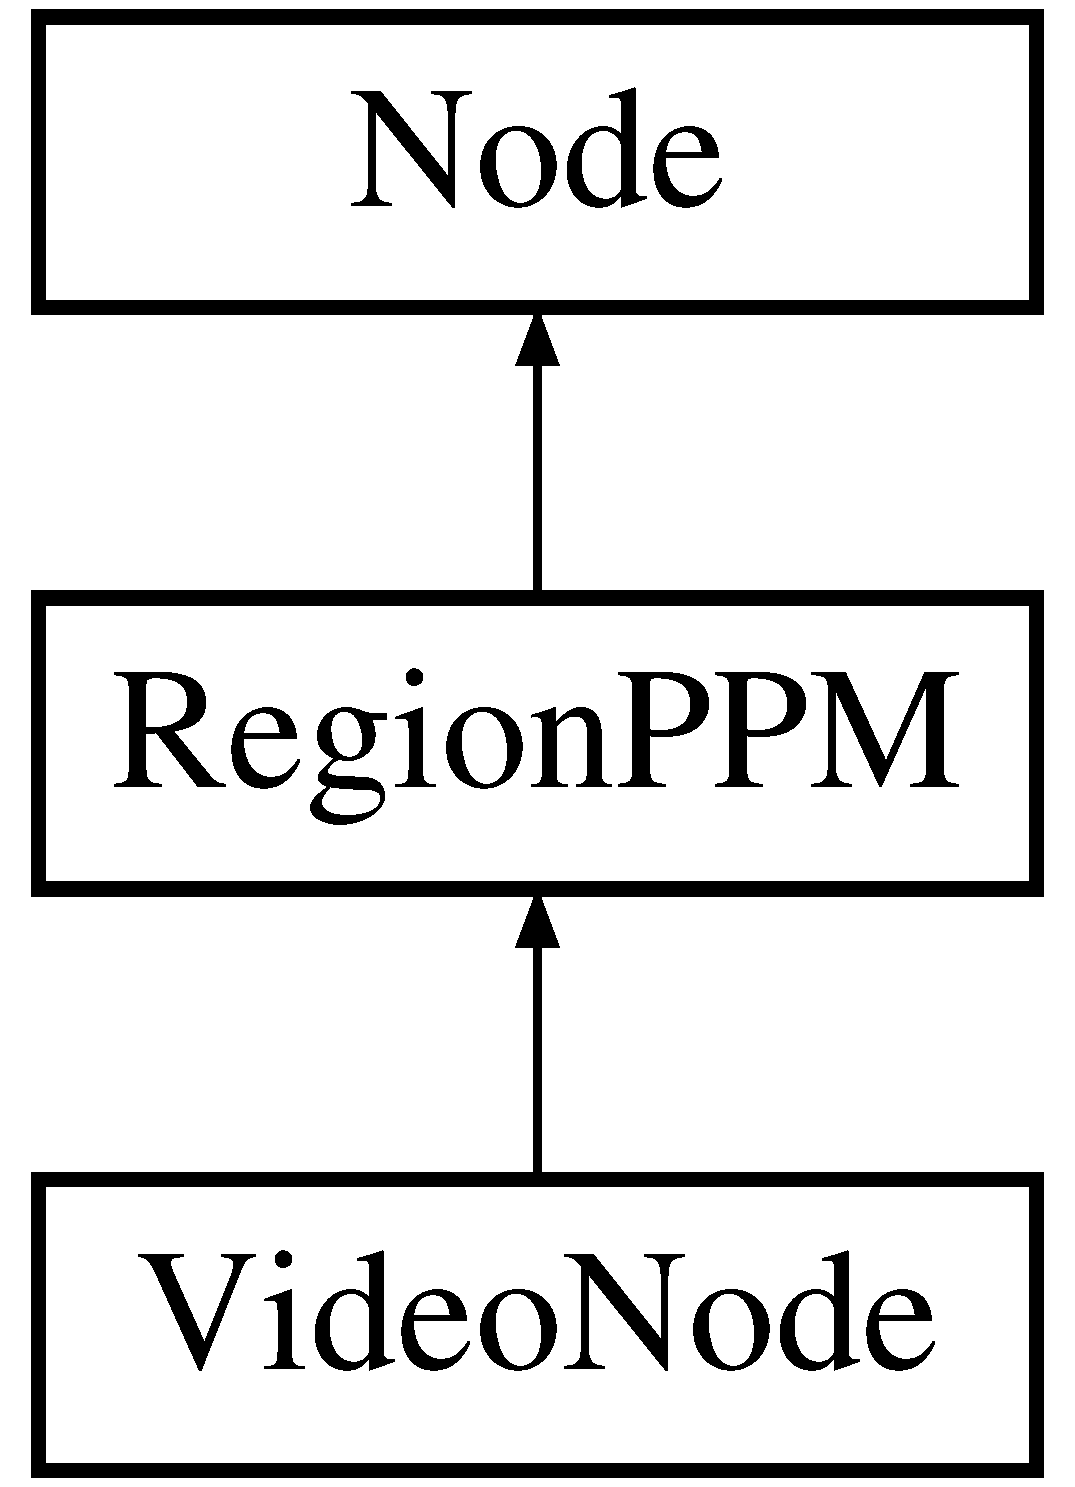
\includegraphics[height=3cm]{classVideoNode}
\end{center}
\end{figure}
\subsection*{Public Member Functions}
\begin{CompactItemize}
\item 
{\bf BeliefPtr} {\bf getGlobalBlfPtr} ()
\item 
void {\bf setGlobalBlfPtr} ({\bf BeliefPtr} bptr)
\item 
void {\bf setOldState} ({\bf StatePtr} s)
\item 
{\bf StatePtr} {\bf getOldState} ()
\item 
bool {\bf addAugmentCand} ({\bf StatePtr} sptr, {\bf LD} {\bf l})
\item 
void {\bf finalizeCands} ({\bf StatePtr} sO)
\item 
void {\bf setNextStateCandMp} (NEXT\_\-CAND\_\-MP mp)
\item 
NEXT\_\-CAND\_\-MP {\bf getNextStateCandMp} ()
\item 
void {\bf setCPTR} ({\bf ConditionalBeliefPtr} \_\-cptr)
\item 
{\bf ConditionalBeliefPtr} {\bf getCPTR} ()
\item 
{\bf VideoNode} (string {\bf id})
\item 
virtual {\bf $\sim$VideoNode} ()
\end{CompactItemize}
\subsection*{Static Public Member Functions}
\begin{CompactItemize}
\item 
static vector$<$ int $>$ {\bf getIntFromId} (string s)
\item 
static bool {\bf isInterior} (int {\bf x}, int {\bf y}, string sBig)
\begin{CompactList}\small\item\em checks whether block is interior \item\end{CompactList}\item 
static bool {\bf isSubset} (string sSmall, string sBig)
\item 
static string {\bf intersection} (string s1, string s2)
\item 
static string {\bf getIdFromInt} (int {\bf x}, int {\bf y}, int {\bf l}, int {\bf w})
\end{CompactItemize}
\subsection*{Public Attributes}
\begin{CompactItemize}
\item 
{\bf BeliefPtr} {\bf localBlfPtr}
\item 
{\bf ConditionalBeliefPtr} {\bf localCondBlfPtr}
\item 
bool {\bf isMasked}
\begin{CompactList}\small\item\em is masked \item\end{CompactList}\item 
map$<$ {\bf StatePtr}, {\bf LD}, {\bf StatePtrCmp} $>$ {\bf nextStateMp}
\item 
map$<$ {\bf StatePtr}, {\bf LD}, {\bf StatePtrCmp} $>$ {\bf augmentsMp}
\end{CompactItemize}
\subsection*{Private Attributes}
\begin{CompactItemize}
\item 
{\bf ConditionalBeliefPtr} {\bf globalCondPtr}
\begin{CompactList}\small\item\em the global conditional belief pointer of appropriate size \item\end{CompactList}\item 
int {\bf cr}
\begin{CompactList}\small\item\em the block counting number \item\end{CompactList}\item 
int {\bf x}
\begin{CompactList}\small\item\em dimensions of the block \item\end{CompactList}\item 
int {\bf y}
\item 
int {\bf l}
\item 
int {\bf w}
\item 
{\bf BeliefPtr} {\bf globalBlfPtr}
\begin{CompactList}\small\item\em the global belief pointer of appropriate size; \item\end{CompactList}\item 
{\bf StatePtr} {\bf sOld}
\begin{CompactList}\small\item\em the original state \item\end{CompactList}\end{CompactItemize}


\subsection{Constructor \& Destructor Documentation}
\index{VideoNode@{VideoNode}!VideoNode@{VideoNode}}
\index{VideoNode@{VideoNode}!VideoNode@{VideoNode}}
\subsubsection{\setlength{\rightskip}{0pt plus 5cm}VideoNode::VideoNode (string {\em id})}\label{classVideoNode_72b54fe609deac90c40acb51b2e68c76}


\index{VideoNode@{VideoNode}!~VideoNode@{$\sim$VideoNode}}
\index{~VideoNode@{$\sim$VideoNode}!VideoNode@{VideoNode}}
\subsubsection{\setlength{\rightskip}{0pt plus 5cm}VideoNode::$\sim$VideoNode ()\hspace{0.3cm}{\tt  [virtual]}}\label{classVideoNode_5ff98f195450b74e879fbc393a8a3cb2}




\subsection{Member Function Documentation}
\index{VideoNode@{VideoNode}!getGlobalBlfPtr@{getGlobalBlfPtr}}
\index{getGlobalBlfPtr@{getGlobalBlfPtr}!VideoNode@{VideoNode}}
\subsubsection{\setlength{\rightskip}{0pt plus 5cm}{\bf BeliefPtr} VideoNode::getGlobalBlfPtr ()\hspace{0.3cm}{\tt  [inline]}}\label{classVideoNode_ded48b3d52c23969ef2a32354fd766e6}


\index{VideoNode@{VideoNode}!setGlobalBlfPtr@{setGlobalBlfPtr}}
\index{setGlobalBlfPtr@{setGlobalBlfPtr}!VideoNode@{VideoNode}}
\subsubsection{\setlength{\rightskip}{0pt plus 5cm}void VideoNode::setGlobalBlfPtr ({\bf BeliefPtr} {\em bptr})\hspace{0.3cm}{\tt  [inline]}}\label{classVideoNode_c704a589284f793f9a3943a515a45dff}


\index{VideoNode@{VideoNode}!setOldState@{setOldState}}
\index{setOldState@{setOldState}!VideoNode@{VideoNode}}
\subsubsection{\setlength{\rightskip}{0pt plus 5cm}void VideoNode::setOldState ({\bf StatePtr} {\em s})\hspace{0.3cm}{\tt  [inline]}}\label{classVideoNode_91e4381a8e730638ede819fa02df95c1}


\index{VideoNode@{VideoNode}!getOldState@{getOldState}}
\index{getOldState@{getOldState}!VideoNode@{VideoNode}}
\subsubsection{\setlength{\rightskip}{0pt plus 5cm}{\bf StatePtr} VideoNode::getOldState ()\hspace{0.3cm}{\tt  [inline]}}\label{classVideoNode_ce263c192348ad89b3cfab4860542742}


\index{VideoNode@{VideoNode}!addAugmentCand@{addAugmentCand}}
\index{addAugmentCand@{addAugmentCand}!VideoNode@{VideoNode}}
\subsubsection{\setlength{\rightskip}{0pt plus 5cm}bool VideoNode::addAugmentCand ({\bf StatePtr} {\em sptr}, {\bf LD} {\em l})\hspace{0.3cm}{\tt  [inline]}}\label{classVideoNode_e3701f6a13fe06322a97c876d95d7688}


\index{VideoNode@{VideoNode}!finalizeCands@{finalizeCands}}
\index{finalizeCands@{finalizeCands}!VideoNode@{VideoNode}}
\subsubsection{\setlength{\rightskip}{0pt plus 5cm}void VideoNode::finalizeCands ({\bf StatePtr} {\em sO})}\label{classVideoNode_11bd4362c71da7fc4846a4e9a4db2b63}


\index{VideoNode@{VideoNode}!setNextStateCandMp@{setNextStateCandMp}}
\index{setNextStateCandMp@{setNextStateCandMp}!VideoNode@{VideoNode}}
\subsubsection{\setlength{\rightskip}{0pt plus 5cm}void VideoNode::setNextStateCandMp (NEXT\_\-CAND\_\-MP {\em mp})\hspace{0.3cm}{\tt  [inline]}}\label{classVideoNode_d2889936b0b6aadb8309d770918e5d2c}


\index{VideoNode@{VideoNode}!getNextStateCandMp@{getNextStateCandMp}}
\index{getNextStateCandMp@{getNextStateCandMp}!VideoNode@{VideoNode}}
\subsubsection{\setlength{\rightskip}{0pt plus 5cm}NEXT\_\-CAND\_\-MP VideoNode::getNextStateCandMp ()\hspace{0.3cm}{\tt  [inline]}}\label{classVideoNode_6914915d89723d02f7d98f2d10fc35a5}


\index{VideoNode@{VideoNode}!setCPTR@{setCPTR}}
\index{setCPTR@{setCPTR}!VideoNode@{VideoNode}}
\subsubsection{\setlength{\rightskip}{0pt plus 5cm}void VideoNode::setCPTR ({\bf ConditionalBeliefPtr} {\em \_\-cptr})\hspace{0.3cm}{\tt  [inline]}}\label{classVideoNode_f10f47881643c17c12dc928a099c7bd7}


\index{VideoNode@{VideoNode}!getCPTR@{getCPTR}}
\index{getCPTR@{getCPTR}!VideoNode@{VideoNode}}
\subsubsection{\setlength{\rightskip}{0pt plus 5cm}{\bf ConditionalBeliefPtr} VideoNode::getCPTR ()\hspace{0.3cm}{\tt  [inline]}}\label{classVideoNode_ed4e0fa3b5b1f969019bc415db657ca6}


\index{VideoNode@{VideoNode}!getIntFromId@{getIntFromId}}
\index{getIntFromId@{getIntFromId}!VideoNode@{VideoNode}}
\subsubsection{\setlength{\rightskip}{0pt plus 5cm}vector$<$ int $>$ VideoNode::getIntFromId (string {\em s})\hspace{0.3cm}{\tt  [static]}}\label{classVideoNode_e02f9db961acbb056812d63f1ac67428}


\index{VideoNode@{VideoNode}!isInterior@{isInterior}}
\index{isInterior@{isInterior}!VideoNode@{VideoNode}}
\subsubsection{\setlength{\rightskip}{0pt plus 5cm}bool VideoNode::isInterior (int {\em x}, int {\em y}, string {\em sBig})\hspace{0.3cm}{\tt  [static]}}\label{classVideoNode_4ff21a96c68156ec5b18afdbd98ea0bc}


checks whether block is interior 

\index{VideoNode@{VideoNode}!isSubset@{isSubset}}
\index{isSubset@{isSubset}!VideoNode@{VideoNode}}
\subsubsection{\setlength{\rightskip}{0pt plus 5cm}bool VideoNode::isSubset (string {\em sSmall}, string {\em sBig})\hspace{0.3cm}{\tt  [static]}}\label{classVideoNode_caa3921526d3d5c4ad4c171ac72241b6}


\index{VideoNode@{VideoNode}!intersection@{intersection}}
\index{intersection@{intersection}!VideoNode@{VideoNode}}
\subsubsection{\setlength{\rightskip}{0pt plus 5cm}string VideoNode::intersection (string {\em s1}, string {\em s2})\hspace{0.3cm}{\tt  [static]}}\label{classVideoNode_2995399e235f91ace15a87dab03adb55}


returns the block that is common between s1 and s2 \index{VideoNode@{VideoNode}!getIdFromInt@{getIdFromInt}}
\index{getIdFromInt@{getIdFromInt}!VideoNode@{VideoNode}}
\subsubsection{\setlength{\rightskip}{0pt plus 5cm}static string VideoNode::getIdFromInt (int {\em x}, int {\em y}, int {\em l}, int {\em w})\hspace{0.3cm}{\tt  [inline, static]}}\label{classVideoNode_9bac8077cc6f931679e524f70870de76}




\subsection{Member Data Documentation}
\index{VideoNode@{VideoNode}!globalCondPtr@{globalCondPtr}}
\index{globalCondPtr@{globalCondPtr}!VideoNode@{VideoNode}}
\subsubsection{\setlength{\rightskip}{0pt plus 5cm}{\bf ConditionalBeliefPtr} {\bf VideoNode::globalCondPtr}\hspace{0.3cm}{\tt  [private]}}\label{classVideoNode_c35636979ade93f63cde7ea655e318e0}


the global conditional belief pointer of appropriate size 

\index{VideoNode@{VideoNode}!cr@{cr}}
\index{cr@{cr}!VideoNode@{VideoNode}}
\subsubsection{\setlength{\rightskip}{0pt plus 5cm}int {\bf VideoNode::cr}\hspace{0.3cm}{\tt  [private]}}\label{classVideoNode_07fc09cceeaf0bfef6690aecdb2a5574}


the block counting number 



Reimplemented from {\bf RegionPPM} \doxyref{}{p.}{classRegionPPM_c21f25cb3cd95ae5717909badbb7014a}.\index{VideoNode@{VideoNode}!x@{x}}
\index{x@{x}!VideoNode@{VideoNode}}
\subsubsection{\setlength{\rightskip}{0pt plus 5cm}int {\bf VideoNode::x}\hspace{0.3cm}{\tt  [private]}}\label{classVideoNode_0bae4457bb6ef95b25ef3007b67eebbf}


dimensions of the block 

\index{VideoNode@{VideoNode}!y@{y}}
\index{y@{y}!VideoNode@{VideoNode}}
\subsubsection{\setlength{\rightskip}{0pt plus 5cm}int {\bf VideoNode::y}\hspace{0.3cm}{\tt  [private]}}\label{classVideoNode_4f91639167db6a1fe2e375a1166fa339}


\index{VideoNode@{VideoNode}!l@{l}}
\index{l@{l}!VideoNode@{VideoNode}}
\subsubsection{\setlength{\rightskip}{0pt plus 5cm}int {\bf VideoNode::l}\hspace{0.3cm}{\tt  [private]}}\label{classVideoNode_897fda12dcd859f64d901bb310aefbaa}


\index{VideoNode@{VideoNode}!w@{w}}
\index{w@{w}!VideoNode@{VideoNode}}
\subsubsection{\setlength{\rightskip}{0pt plus 5cm}int {\bf VideoNode::w}\hspace{0.3cm}{\tt  [private]}}\label{classVideoNode_5653685b4e36e5d617e5b28758844c04}


\index{VideoNode@{VideoNode}!globalBlfPtr@{globalBlfPtr}}
\index{globalBlfPtr@{globalBlfPtr}!VideoNode@{VideoNode}}
\subsubsection{\setlength{\rightskip}{0pt plus 5cm}{\bf BeliefPtr} {\bf VideoNode::globalBlfPtr}\hspace{0.3cm}{\tt  [private]}}\label{classVideoNode_7dea28e600c60808ec170c03a0d9eb7a}


the global belief pointer of appropriate size; 

\index{VideoNode@{VideoNode}!sOld@{sOld}}
\index{sOld@{sOld}!VideoNode@{VideoNode}}
\subsubsection{\setlength{\rightskip}{0pt plus 5cm}{\bf StatePtr} {\bf VideoNode::sOld}\hspace{0.3cm}{\tt  [private]}}\label{classVideoNode_db740a1b91e1ebe70dc1e4a26da0eac2}


the original state 

\index{VideoNode@{VideoNode}!localBlfPtr@{localBlfPtr}}
\index{localBlfPtr@{localBlfPtr}!VideoNode@{VideoNode}}
\subsubsection{\setlength{\rightskip}{0pt plus 5cm}{\bf BeliefPtr} {\bf VideoNode::localBlfPtr}}\label{classVideoNode_cb639d57227bafac088ea375431179fd}


\index{VideoNode@{VideoNode}!localCondBlfPtr@{localCondBlfPtr}}
\index{localCondBlfPtr@{localCondBlfPtr}!VideoNode@{VideoNode}}
\subsubsection{\setlength{\rightskip}{0pt plus 5cm}{\bf ConditionalBeliefPtr} {\bf VideoNode::localCondBlfPtr}}\label{classVideoNode_458fe9e71bd5c36c6b2f04e6213f4d54}


\index{VideoNode@{VideoNode}!isMasked@{isMasked}}
\index{isMasked@{isMasked}!VideoNode@{VideoNode}}
\subsubsection{\setlength{\rightskip}{0pt plus 5cm}bool {\bf VideoNode::isMasked}}\label{classVideoNode_88700ff0b59eef55130a2cff5a87fc76}


is masked 

\index{VideoNode@{VideoNode}!nextStateMp@{nextStateMp}}
\index{nextStateMp@{nextStateMp}!VideoNode@{VideoNode}}
\subsubsection{\setlength{\rightskip}{0pt plus 5cm}map$<${\bf StatePtr}, {\bf LD}, {\bf StatePtrCmp}$>$ {\bf VideoNode::nextStateMp}}\label{classVideoNode_8e74703e49899c0fe083eb1b021a995c}


\index{VideoNode@{VideoNode}!augmentsMp@{augmentsMp}}
\index{augmentsMp@{augmentsMp}!VideoNode@{VideoNode}}
\subsubsection{\setlength{\rightskip}{0pt plus 5cm}map$<${\bf StatePtr}, {\bf LD}, {\bf StatePtrCmp}$>$ {\bf VideoNode::augmentsMp}}\label{classVideoNode_705607f18e7be40337312ced2202c429}




The documentation for this class was generated from the following files:\begin{CompactItemize}
\item 
inc/{\bf VideoNode.h}\item 
src/{\bf VideoNode.cpp}\end{CompactItemize}

\section{VideoReader Class Reference}
\label{classVideoReader}\index{VideoReader@{VideoReader}}
{\tt \#include $<$VideoReader.h$>$}

\subsection*{Public Member Functions}
\begin{CompactItemize}
\item 
void {\bf setGraph} ({\bf VideoGraph} $\ast$\_\-g)
\item 
int {\bf getN1} ()
\item 
int {\bf getN2} ()
\item 
void {\bf setGrayScale} (bool \_\-isGray)
\item 
void {\bf setNumLvls} (int s)
\item 
{\bf VideoReader} (bool \_\-gray=true, int \_\-numLvls=8)
\item 
IplImage $\ast$ {\bf getCurrentFrame} (CvCapture $\ast$currVideo)
\begin{CompactList}\small\item\em returns the current frame \item\end{CompactList}\item 
void {\bf openVideo} (string videoName)
\begin{CompactList}\small\item\em opens a video \item\end{CompactList}\item 
void {\bf runMain} (bool gray=true, int {\bf numLvls}=4, int maxNum=-1, int priorNum=5, int frameJump=1)
\begin{CompactList}\small\item\em the main engine that updates all the three engines \item\end{CompactList}\item 
bool {\bf convertInputFrame} (bool gray=true, int {\bf numLvls}=4)
\begin{CompactList}\small\item\em this function just displays the next frame of the input video until no more to display \item\end{CompactList}\item 
void {\bf updateOutputVideo} ()
\begin{CompactList}\small\item\em this function is recursively called until all the video holes have been filled \item\end{CompactList}\item 
virtual {\bf $\sim$VideoReader} ()
\item 
vector$<$ {\bf INT} $>$ {\bf getDataFromFrame} (IplImage $\ast${\bf frame}, int x, int y, int r, int c)
\begin{CompactList}\small\item\em get the data for block of pixels \item\end{CompactList}\item 
bool {\bf isValidPixel} (IplImage $\ast${\bf frame}, int x, int y)
\begin{CompactList}\small\item\em checks for validity of pixel in frame size \item\end{CompactList}\item 
void {\bf updateLastFrame} (IplImage $\ast${\bf frame}=NULL)
\begin{CompactList}\small\item\em updates the last frame \item\end{CompactList}\item 
void {\bf display} ()
\item 
double {\bf getFrameDifference} (IplImage $\ast${\bf frame1}, IplImage $\ast$frame2, IplImage $\ast$resFrame=NULL, int $\ast$NP=NULL)
\item 
void {\bf initPrevFrames} (int N)
\item 
void {\bf updateMaskFrame} (int x, int y, int l, int w)
\item 
void {\bf updatePrevFrames} (IplImage $\ast${\bf frame}, int N)
\item 
void {\bf overlapFrame} (IplImage $\ast$inpainted, IplImage $\ast$input, IplImage $\ast$res\_\-frame)
\item 
void {\bf runFC} (bool gray, int {\bf numLvls}, int maxNum, int priorNum, int frameJump)
\item 
void {\bf runInPaint} ()
\item 
void {\bf getMissingMask} (IplImage $\ast${\bf mask\_\-frame}, {\bf LD} probMissing)
\item 
void {\bf updateBasedOnPrevFrames} (IplImage $\ast${\bf mask\_\-frame})
\item 
void {\bf runNoisy} (bool gray, int {\bf numLvls}, int maxNum, int priorNum, int frameJump)
\item 
void {\bf updateInputFrame} (IplImage $\ast${\bf input\_\-frame}, IplImage $\ast$curr\_\-mask)
\item 
bool {\bf incrementFrame} (IplImage $\ast$pastFrame, IplImage $\ast$nextFrame)
\item 
void {\bf writeOp} (int count)
\end{CompactItemize}
\subsection*{Public Attributes}
\begin{CompactItemize}
\item 
IplImage $\ast$ {\bf frame}
\begin{CompactList}\small\item\em temporary frames used for conversion \item\end{CompactList}\item 
IplImage $\ast$ {\bf frame1}
\item 
IplImage $\ast$ {\bf frame1\_\-1C}
\item 
IplImage $\ast$ {\bf frame2\_\-GS}
\item 
CvSize {\bf frame\_\-size}
\begin{CompactList}\small\item\em frame size of the video \item\end{CompactList}\item 
IplImage $\ast$ {\bf last\_\-frame}
\begin{CompactList}\small\item\em the last frame \item\end{CompactList}\item 
IplImage $\ast$ {\bf input\_\-frame}
\begin{CompactList}\small\item\em the default pointer to the current frame \item\end{CompactList}\item 
IplImage $\ast$ {\bf output\_\-frame}
\begin{CompactList}\small\item\em pointer to the output frame \item\end{CompactList}\item 
IplImage $\ast$ {\bf mask\_\-frame}
\begin{CompactList}\small\item\em pointer to the mask frame \item\end{CompactList}\item 
CvCapture $\ast$ {\bf input\_\-video}
\begin{CompactList}\small\item\em the default pointer to the current video \item\end{CompactList}\end{CompactItemize}
\subsection*{Private Attributes}
\begin{CompactItemize}
\item 
int {\bf frame\_\-count}
\begin{CompactList}\small\item\em frame count \item\end{CompactList}\item 
bool {\bf grayscale}
\begin{CompactList}\small\item\em whether to do the inference on bw or color \item\end{CompactList}\item 
int {\bf numLvls}
\begin{CompactList}\small\item\em the maximum value each pixel can take 0...maxgrayscale (default 255) \item\end{CompactList}\item 
int {\bf rwidth}
\begin{CompactList}\small\item\em biggest region width \item\end{CompactList}\item 
int {\bf rheight}
\begin{CompactList}\small\item\em biggest region height \item\end{CompactList}\item 
int {\bf xoverlap}
\begin{CompactList}\small\item\em horizontal overlap between adjoining biggest regions \item\end{CompactList}\item 
int {\bf yoverlap}
\begin{CompactList}\small\item\em vertical overlap between adjoining biggest regions \item\end{CompactList}\item 
IplImage $\ast$ {\bf diff\_\-frame}
\begin{CompactList}\small\item\em pointer to the difference frame \item\end{CompactList}\item 
void $\ast$ {\bf last\_\-frame\_\-window\_\-handle}
\item 
void $\ast$ {\bf input\_\-window\_\-handle}
\begin{CompactList}\small\item\em pointer to the default window \item\end{CompactList}\item 
void $\ast$ {\bf output\_\-window\_\-handle}
\begin{CompactList}\small\item\em pointer to the output window \item\end{CompactList}\item 
void $\ast$ {\bf mask\_\-window\_\-handle}
\begin{CompactList}\small\item\em pointer to the mask frame \item\end{CompactList}\item 
long {\bf number\_\-of\_\-frames}
\begin{CompactList}\small\item\em number of frames in the video sequence \item\end{CompactList}\item 
int {\bf frames\_\-per\_\-second}
\begin{CompactList}\small\item\em number of frames per second \item\end{CompactList}\item 
{\bf VideoGraph} $\ast$ {\bf graph}
\begin{CompactList}\small\item\em the graph used for inference \item\end{CompactList}\item 
CvVideoWriter $\ast$ {\bf output\_\-video}
\item 
CvVideoWriter $\ast$ {\bf difference\_\-video}
\item 
vector$<$ IplImage $\ast$ $>$ {\bf prev\_\-frames}
\item 
int {\bf count11}
\end{CompactItemize}


\subsection{Detailed Description}
This class handles all interactions with the video data 



\subsection{Constructor \& Destructor Documentation}
\index{VideoReader@{VideoReader}!VideoReader@{VideoReader}}
\index{VideoReader@{VideoReader}!VideoReader@{VideoReader}}
\subsubsection{\setlength{\rightskip}{0pt plus 5cm}VideoReader::VideoReader (bool {\em \_\-gray} = {\tt true}, int {\em \_\-numLvls} = {\tt 8})}\label{classVideoReader_1c44fe2505e7190ee4421c0c4553d74d}


\index{VideoReader@{VideoReader}!~VideoReader@{$\sim$VideoReader}}
\index{~VideoReader@{$\sim$VideoReader}!VideoReader@{VideoReader}}
\subsubsection{\setlength{\rightskip}{0pt plus 5cm}VideoReader::$\sim$VideoReader ()\hspace{0.3cm}{\tt  [virtual]}}\label{classVideoReader_901bd17be9cb209d23bf9d5b7087b91d}




\subsection{Member Function Documentation}
\index{VideoReader@{VideoReader}!setGraph@{setGraph}}
\index{setGraph@{setGraph}!VideoReader@{VideoReader}}
\subsubsection{\setlength{\rightskip}{0pt plus 5cm}void VideoReader::setGraph ({\bf VideoGraph} $\ast$ {\em \_\-g})\hspace{0.3cm}{\tt  [inline]}}\label{classVideoReader_ebe8e6e685f96dac03656b5ae4ce33eb}


\index{VideoReader@{VideoReader}!getN1@{getN1}}
\index{getN1@{getN1}!VideoReader@{VideoReader}}
\subsubsection{\setlength{\rightskip}{0pt plus 5cm}int VideoReader::getN1 ()\hspace{0.3cm}{\tt  [inline]}}\label{classVideoReader_e4b10f575c7ebea798adc760e050f0fb}


\index{VideoReader@{VideoReader}!getN2@{getN2}}
\index{getN2@{getN2}!VideoReader@{VideoReader}}
\subsubsection{\setlength{\rightskip}{0pt plus 5cm}int VideoReader::getN2 ()\hspace{0.3cm}{\tt  [inline]}}\label{classVideoReader_a05ae0af66423566ab965c337403d955}


\index{VideoReader@{VideoReader}!setGrayScale@{setGrayScale}}
\index{setGrayScale@{setGrayScale}!VideoReader@{VideoReader}}
\subsubsection{\setlength{\rightskip}{0pt plus 5cm}void VideoReader::setGrayScale (bool {\em \_\-isGray})\hspace{0.3cm}{\tt  [inline]}}\label{classVideoReader_797a9ecb59a69145c074b7414af3ef12}


\index{VideoReader@{VideoReader}!setNumLvls@{setNumLvls}}
\index{setNumLvls@{setNumLvls}!VideoReader@{VideoReader}}
\subsubsection{\setlength{\rightskip}{0pt plus 5cm}void VideoReader::setNumLvls (int {\em s})\hspace{0.3cm}{\tt  [inline]}}\label{classVideoReader_0882334d0d49bb404faf5eedf06ffa5c}


\index{VideoReader@{VideoReader}!getCurrentFrame@{getCurrentFrame}}
\index{getCurrentFrame@{getCurrentFrame}!VideoReader@{VideoReader}}
\subsubsection{\setlength{\rightskip}{0pt plus 5cm}IplImage$\ast$ VideoReader::getCurrentFrame (CvCapture $\ast$ {\em currVideo})}\label{classVideoReader_cd5d16555d3bfde02fc99653ca4419cd}


returns the current frame 

\index{VideoReader@{VideoReader}!openVideo@{openVideo}}
\index{openVideo@{openVideo}!VideoReader@{VideoReader}}
\subsubsection{\setlength{\rightskip}{0pt plus 5cm}void VideoReader::openVideo (string {\em videoName})}\label{classVideoReader_adc3521b176c93d1530f46c3a1f1cf3a}


opens a video 

\index{VideoReader@{VideoReader}!runMain@{runMain}}
\index{runMain@{runMain}!VideoReader@{VideoReader}}
\subsubsection{\setlength{\rightskip}{0pt plus 5cm}void VideoReader::runMain (bool {\em gray} = {\tt true}, int {\em numLvls} = {\tt 4}, int {\em maxNum} = {\tt -1}, int {\em priorNum} = {\tt 5}, int {\em frameJump} = {\tt 1})}\label{classVideoReader_7d3f6428ad3227214553385f1b4eb42a}


the main engine that updates all the three engines 

\index{VideoReader@{VideoReader}!convertInputFrame@{convertInputFrame}}
\index{convertInputFrame@{convertInputFrame}!VideoReader@{VideoReader}}
\subsubsection{\setlength{\rightskip}{0pt plus 5cm}bool VideoReader::convertInputFrame (bool {\em gray} = {\tt true}, int {\em numLvls} = {\tt 4})}\label{classVideoReader_58b0f6af53127781dcba478ea6f3608c}


this function just displays the next frame of the input video until no more to display 

\index{VideoReader@{VideoReader}!updateOutputVideo@{updateOutputVideo}}
\index{updateOutputVideo@{updateOutputVideo}!VideoReader@{VideoReader}}
\subsubsection{\setlength{\rightskip}{0pt plus 5cm}void VideoReader::updateOutputVideo ()}\label{classVideoReader_cad516b891d8ad1c792734c76906de3e}


this function is recursively called until all the video holes have been filled 

\index{VideoReader@{VideoReader}!getDataFromFrame@{getDataFromFrame}}
\index{getDataFromFrame@{getDataFromFrame}!VideoReader@{VideoReader}}
\subsubsection{\setlength{\rightskip}{0pt plus 5cm}vector$<$ {\bf INT} $>$ VideoReader::getDataFromFrame (IplImage $\ast$ {\em frame}, int {\em x}, int {\em y}, int {\em r}, int {\em c})}\label{classVideoReader_e458f2b3d47bfc1750092716ce082fb8}


get the data for block of pixels 

\index{VideoReader@{VideoReader}!isValidPixel@{isValidPixel}}
\index{isValidPixel@{isValidPixel}!VideoReader@{VideoReader}}
\subsubsection{\setlength{\rightskip}{0pt plus 5cm}bool VideoReader::isValidPixel (IplImage $\ast$ {\em frame}, int {\em x}, int {\em y})\hspace{0.3cm}{\tt  [inline]}}\label{classVideoReader_c905f0c4bc9325bf319d746ebcdd8ce7}


checks for validity of pixel in frame size 

\index{VideoReader@{VideoReader}!updateLastFrame@{updateLastFrame}}
\index{updateLastFrame@{updateLastFrame}!VideoReader@{VideoReader}}
\subsubsection{\setlength{\rightskip}{0pt plus 5cm}void VideoReader::updateLastFrame (IplImage $\ast$ {\em frame} = {\tt NULL})}\label{classVideoReader_f89a1037188cb805123b56ff56bed90f}


updates the last frame 

\index{VideoReader@{VideoReader}!display@{display}}
\index{display@{display}!VideoReader@{VideoReader}}
\subsubsection{\setlength{\rightskip}{0pt plus 5cm}void VideoReader::display ()}\label{classVideoReader_fc9f0afccdb05c79391718c7f9cce7a2}


\index{VideoReader@{VideoReader}!getFrameDifference@{getFrameDifference}}
\index{getFrameDifference@{getFrameDifference}!VideoReader@{VideoReader}}
\subsubsection{\setlength{\rightskip}{0pt plus 5cm}double VideoReader::getFrameDifference (IplImage $\ast$ {\em frame1}, IplImage $\ast$ {\em frame2}, IplImage $\ast$ {\em resFrame} = {\tt NULL}, int $\ast$ {\em NP} = {\tt NULL})}\label{classVideoReader_08d89437b44ac917fa389a7f1b865f81}


\index{VideoReader@{VideoReader}!initPrevFrames@{initPrevFrames}}
\index{initPrevFrames@{initPrevFrames}!VideoReader@{VideoReader}}
\subsubsection{\setlength{\rightskip}{0pt plus 5cm}void VideoReader::initPrevFrames (int {\em N})}\label{classVideoReader_63c948f1bdafb9aa1440b65f41f43199}


\index{VideoReader@{VideoReader}!updateMaskFrame@{updateMaskFrame}}
\index{updateMaskFrame@{updateMaskFrame}!VideoReader@{VideoReader}}
\subsubsection{\setlength{\rightskip}{0pt plus 5cm}void VideoReader::updateMaskFrame (int {\em x}, int {\em y}, int {\em l}, int {\em w})}\label{classVideoReader_d134c1d615262e4e2c14af19151969e4}


\index{VideoReader@{VideoReader}!updatePrevFrames@{updatePrevFrames}}
\index{updatePrevFrames@{updatePrevFrames}!VideoReader@{VideoReader}}
\subsubsection{\setlength{\rightskip}{0pt plus 5cm}void VideoReader::updatePrevFrames (IplImage $\ast$ {\em frame}, int {\em N})\hspace{0.3cm}{\tt  [inline]}}\label{classVideoReader_b9828f954dbbbe5d7ff5dfba64dfc3b2}


\index{VideoReader@{VideoReader}!overlapFrame@{overlapFrame}}
\index{overlapFrame@{overlapFrame}!VideoReader@{VideoReader}}
\subsubsection{\setlength{\rightskip}{0pt plus 5cm}void VideoReader::overlapFrame (IplImage $\ast$ {\em inpainted}, IplImage $\ast$ {\em input}, IplImage $\ast$ {\em res\_\-frame})}\label{classVideoReader_f3d0da2e6684bc12baba5adb44e6f0c6}


\index{VideoReader@{VideoReader}!runFC@{runFC}}
\index{runFC@{runFC}!VideoReader@{VideoReader}}
\subsubsection{\setlength{\rightskip}{0pt plus 5cm}void VideoReader::runFC (bool {\em gray}, int {\em numLvls}, int {\em maxNum}, int {\em priorNum}, int {\em frameJump})}\label{classVideoReader_db9dca85fe941233dd19136090b95b78}


\index{VideoReader@{VideoReader}!runInPaint@{runInPaint}}
\index{runInPaint@{runInPaint}!VideoReader@{VideoReader}}
\subsubsection{\setlength{\rightskip}{0pt plus 5cm}void VideoReader::runInPaint ()}\label{classVideoReader_29eefb68374172ac39e6f399318cb711}


\index{VideoReader@{VideoReader}!getMissingMask@{getMissingMask}}
\index{getMissingMask@{getMissingMask}!VideoReader@{VideoReader}}
\subsubsection{\setlength{\rightskip}{0pt plus 5cm}void VideoReader::getMissingMask (IplImage $\ast$ {\em mask\_\-frame}, {\bf LD} {\em probMissing})}\label{classVideoReader_75c6a8631b661dbd55caf2fe357ef8f6}


\index{VideoReader@{VideoReader}!updateBasedOnPrevFrames@{updateBasedOnPrevFrames}}
\index{updateBasedOnPrevFrames@{updateBasedOnPrevFrames}!VideoReader@{VideoReader}}
\subsubsection{\setlength{\rightskip}{0pt plus 5cm}void VideoReader::updateBasedOnPrevFrames (IplImage $\ast$ {\em mask\_\-frame})}\label{classVideoReader_ddda11180fc2782c117c30e289d93c2a}


\index{VideoReader@{VideoReader}!runNoisy@{runNoisy}}
\index{runNoisy@{runNoisy}!VideoReader@{VideoReader}}
\subsubsection{\setlength{\rightskip}{0pt plus 5cm}void VideoReader::runNoisy (bool {\em gray}, int {\em numLvls}, int {\em maxNum}, int {\em priorNum}, int {\em frameJump})}\label{classVideoReader_ffbcf0d37d2bb67edd64cb6317bf4e5b}


\index{VideoReader@{VideoReader}!updateInputFrame@{updateInputFrame}}
\index{updateInputFrame@{updateInputFrame}!VideoReader@{VideoReader}}
\subsubsection{\setlength{\rightskip}{0pt plus 5cm}void VideoReader::updateInputFrame (IplImage $\ast$ {\em input\_\-frame}, IplImage $\ast$ {\em curr\_\-mask})}\label{classVideoReader_00913618c64f5057770c195d72f7d45c}


\index{VideoReader@{VideoReader}!incrementFrame@{incrementFrame}}
\index{incrementFrame@{incrementFrame}!VideoReader@{VideoReader}}
\subsubsection{\setlength{\rightskip}{0pt plus 5cm}bool VideoReader::incrementFrame (IplImage $\ast$ {\em pastFrame}, IplImage $\ast$ {\em nextFrame})\hspace{0.3cm}{\tt  [inline]}}\label{classVideoReader_aa784ab08706bbaf9fa6bdfee0730c3d}


\index{VideoReader@{VideoReader}!writeOp@{writeOp}}
\index{writeOp@{writeOp}!VideoReader@{VideoReader}}
\subsubsection{\setlength{\rightskip}{0pt plus 5cm}void VideoReader::writeOp (int {\em count})\hspace{0.3cm}{\tt  [inline]}}\label{classVideoReader_3fc9ed897920438db26fc0763810da2e}




\subsection{Member Data Documentation}
\index{VideoReader@{VideoReader}!frame_count@{frame\_\-count}}
\index{frame_count@{frame\_\-count}!VideoReader@{VideoReader}}
\subsubsection{\setlength{\rightskip}{0pt plus 5cm}int {\bf VideoReader::frame\_\-count}\hspace{0.3cm}{\tt  [private]}}\label{classVideoReader_2c12827293113d4542eaee2e1198a6d8}


frame count 

\index{VideoReader@{VideoReader}!grayscale@{grayscale}}
\index{grayscale@{grayscale}!VideoReader@{VideoReader}}
\subsubsection{\setlength{\rightskip}{0pt plus 5cm}bool {\bf VideoReader::grayscale}\hspace{0.3cm}{\tt  [private]}}\label{classVideoReader_aa47c27733a214e0c7de038d17788e1c}


whether to do the inference on bw or color 

\index{VideoReader@{VideoReader}!numLvls@{numLvls}}
\index{numLvls@{numLvls}!VideoReader@{VideoReader}}
\subsubsection{\setlength{\rightskip}{0pt plus 5cm}int {\bf VideoReader::numLvls}\hspace{0.3cm}{\tt  [private]}}\label{classVideoReader_e94b623322f96beb6113c7d8bcfc4e54}


the maximum value each pixel can take 0...maxgrayscale (default 255) 

\index{VideoReader@{VideoReader}!rwidth@{rwidth}}
\index{rwidth@{rwidth}!VideoReader@{VideoReader}}
\subsubsection{\setlength{\rightskip}{0pt plus 5cm}int {\bf VideoReader::rwidth}\hspace{0.3cm}{\tt  [private]}}\label{classVideoReader_7a4d7b70657ed12d623cacdf63ec5e18}


biggest region width 

\index{VideoReader@{VideoReader}!rheight@{rheight}}
\index{rheight@{rheight}!VideoReader@{VideoReader}}
\subsubsection{\setlength{\rightskip}{0pt plus 5cm}int {\bf VideoReader::rheight}\hspace{0.3cm}{\tt  [private]}}\label{classVideoReader_ba0220e93ecb9d65d50b9418048c0b92}


biggest region height 

\index{VideoReader@{VideoReader}!xoverlap@{xoverlap}}
\index{xoverlap@{xoverlap}!VideoReader@{VideoReader}}
\subsubsection{\setlength{\rightskip}{0pt plus 5cm}int {\bf VideoReader::xoverlap}\hspace{0.3cm}{\tt  [private]}}\label{classVideoReader_38f091bdf64e9a1ff945bcc8c1f27e66}


horizontal overlap between adjoining biggest regions 

\index{VideoReader@{VideoReader}!yoverlap@{yoverlap}}
\index{yoverlap@{yoverlap}!VideoReader@{VideoReader}}
\subsubsection{\setlength{\rightskip}{0pt plus 5cm}int {\bf VideoReader::yoverlap}\hspace{0.3cm}{\tt  [private]}}\label{classVideoReader_67f9b2d416d5c952555500fe3a26787d}


vertical overlap between adjoining biggest regions 

\index{VideoReader@{VideoReader}!diff_frame@{diff\_\-frame}}
\index{diff_frame@{diff\_\-frame}!VideoReader@{VideoReader}}
\subsubsection{\setlength{\rightskip}{0pt plus 5cm}IplImage$\ast$ {\bf VideoReader::diff\_\-frame}\hspace{0.3cm}{\tt  [private]}}\label{classVideoReader_62cb9a99192ff45b5519e585314b6212}


pointer to the difference frame 

\index{VideoReader@{VideoReader}!last_frame_window_handle@{last\_\-frame\_\-window\_\-handle}}
\index{last_frame_window_handle@{last\_\-frame\_\-window\_\-handle}!VideoReader@{VideoReader}}
\subsubsection{\setlength{\rightskip}{0pt plus 5cm}void$\ast$ {\bf VideoReader::last\_\-frame\_\-window\_\-handle}\hspace{0.3cm}{\tt  [private]}}\label{classVideoReader_eb6402ab96673a345643aae7c5b3abc5}


\index{VideoReader@{VideoReader}!input_window_handle@{input\_\-window\_\-handle}}
\index{input_window_handle@{input\_\-window\_\-handle}!VideoReader@{VideoReader}}
\subsubsection{\setlength{\rightskip}{0pt plus 5cm}void$\ast$ {\bf VideoReader::input\_\-window\_\-handle}\hspace{0.3cm}{\tt  [private]}}\label{classVideoReader_24769274f3320dabba3224c9607c6da1}


pointer to the default window 

\index{VideoReader@{VideoReader}!output_window_handle@{output\_\-window\_\-handle}}
\index{output_window_handle@{output\_\-window\_\-handle}!VideoReader@{VideoReader}}
\subsubsection{\setlength{\rightskip}{0pt plus 5cm}void$\ast$ {\bf VideoReader::output\_\-window\_\-handle}\hspace{0.3cm}{\tt  [private]}}\label{classVideoReader_a2cb69893a34b900bc40442a981ed61b}


pointer to the output window 

\index{VideoReader@{VideoReader}!mask_window_handle@{mask\_\-window\_\-handle}}
\index{mask_window_handle@{mask\_\-window\_\-handle}!VideoReader@{VideoReader}}
\subsubsection{\setlength{\rightskip}{0pt plus 5cm}void$\ast$ {\bf VideoReader::mask\_\-window\_\-handle}\hspace{0.3cm}{\tt  [private]}}\label{classVideoReader_4fa55f836e50a194c81649e279c1fbeb}


pointer to the mask frame 

\index{VideoReader@{VideoReader}!number_of_frames@{number\_\-of\_\-frames}}
\index{number_of_frames@{number\_\-of\_\-frames}!VideoReader@{VideoReader}}
\subsubsection{\setlength{\rightskip}{0pt plus 5cm}long {\bf VideoReader::number\_\-of\_\-frames}\hspace{0.3cm}{\tt  [private]}}\label{classVideoReader_752cb843c271143b3d59aab43bd43450}


number of frames in the video sequence 

\index{VideoReader@{VideoReader}!frames_per_second@{frames\_\-per\_\-second}}
\index{frames_per_second@{frames\_\-per\_\-second}!VideoReader@{VideoReader}}
\subsubsection{\setlength{\rightskip}{0pt plus 5cm}int {\bf VideoReader::frames\_\-per\_\-second}\hspace{0.3cm}{\tt  [private]}}\label{classVideoReader_e89897243c54102536a567325d4040cd}


number of frames per second 

\index{VideoReader@{VideoReader}!graph@{graph}}
\index{graph@{graph}!VideoReader@{VideoReader}}
\subsubsection{\setlength{\rightskip}{0pt plus 5cm}{\bf VideoGraph}$\ast$ {\bf VideoReader::graph}\hspace{0.3cm}{\tt  [private]}}\label{classVideoReader_b7426aebaffee2ae3a8ce0d71f54c0c3}


the graph used for inference 

\index{VideoReader@{VideoReader}!output_video@{output\_\-video}}
\index{output_video@{output\_\-video}!VideoReader@{VideoReader}}
\subsubsection{\setlength{\rightskip}{0pt plus 5cm}CvVideoWriter$\ast$ {\bf VideoReader::output\_\-video}\hspace{0.3cm}{\tt  [private]}}\label{classVideoReader_9d47d64ecb8916b0f6ff0e1a5a739bdb}


\index{VideoReader@{VideoReader}!difference_video@{difference\_\-video}}
\index{difference_video@{difference\_\-video}!VideoReader@{VideoReader}}
\subsubsection{\setlength{\rightskip}{0pt plus 5cm}CvVideoWriter$\ast$ {\bf VideoReader::difference\_\-video}\hspace{0.3cm}{\tt  [private]}}\label{classVideoReader_392113c791a3d66dac3300399a0ee019}


\index{VideoReader@{VideoReader}!prev_frames@{prev\_\-frames}}
\index{prev_frames@{prev\_\-frames}!VideoReader@{VideoReader}}
\subsubsection{\setlength{\rightskip}{0pt plus 5cm}vector$<$IplImage$\ast$ $>$ {\bf VideoReader::prev\_\-frames}\hspace{0.3cm}{\tt  [private]}}\label{classVideoReader_a1414506afefa40ead09b23f1c8231f7}


\index{VideoReader@{VideoReader}!count11@{count11}}
\index{count11@{count11}!VideoReader@{VideoReader}}
\subsubsection{\setlength{\rightskip}{0pt plus 5cm}int {\bf VideoReader::count11}\hspace{0.3cm}{\tt  [private]}}\label{classVideoReader_f28603802a7080dcabf96fa987b0f060}


\index{VideoReader@{VideoReader}!frame@{frame}}
\index{frame@{frame}!VideoReader@{VideoReader}}
\subsubsection{\setlength{\rightskip}{0pt plus 5cm}IplImage$\ast$ {\bf VideoReader::frame}}\label{classVideoReader_25dc6b2a90f7d224a4b0da9dd20cdf59}


temporary frames used for conversion 

\index{VideoReader@{VideoReader}!frame1@{frame1}}
\index{frame1@{frame1}!VideoReader@{VideoReader}}
\subsubsection{\setlength{\rightskip}{0pt plus 5cm}IplImage $\ast$ {\bf VideoReader::frame1}}\label{classVideoReader_d5eacfb8ef1bde674e89051fc912bb5d}


\index{VideoReader@{VideoReader}!frame1_1C@{frame1\_\-1C}}
\index{frame1_1C@{frame1\_\-1C}!VideoReader@{VideoReader}}
\subsubsection{\setlength{\rightskip}{0pt plus 5cm}IplImage $\ast$ {\bf VideoReader::frame1\_\-1C}}\label{classVideoReader_36c0029e5c68e5410ca9d8aac56fd2e6}


\index{VideoReader@{VideoReader}!frame2_GS@{frame2\_\-GS}}
\index{frame2_GS@{frame2\_\-GS}!VideoReader@{VideoReader}}
\subsubsection{\setlength{\rightskip}{0pt plus 5cm}IplImage $\ast$ {\bf VideoReader::frame2\_\-GS}}\label{classVideoReader_09758705a51d09e46b1dca5da0857429}


\index{VideoReader@{VideoReader}!frame_size@{frame\_\-size}}
\index{frame_size@{frame\_\-size}!VideoReader@{VideoReader}}
\subsubsection{\setlength{\rightskip}{0pt plus 5cm}CvSize {\bf VideoReader::frame\_\-size}}\label{classVideoReader_9d640bec746cbcc3ca75b68ce715f094}


frame size of the video 

\index{VideoReader@{VideoReader}!last_frame@{last\_\-frame}}
\index{last_frame@{last\_\-frame}!VideoReader@{VideoReader}}
\subsubsection{\setlength{\rightskip}{0pt plus 5cm}IplImage$\ast$ {\bf VideoReader::last\_\-frame}}\label{classVideoReader_f6c23af4235813a9fa1d506a68cec70c}


the last frame 

\index{VideoReader@{VideoReader}!input_frame@{input\_\-frame}}
\index{input_frame@{input\_\-frame}!VideoReader@{VideoReader}}
\subsubsection{\setlength{\rightskip}{0pt plus 5cm}IplImage$\ast$ {\bf VideoReader::input\_\-frame}}\label{classVideoReader_f93a2ca8f23e7b8f95f55a49176305d1}


the default pointer to the current frame 

\index{VideoReader@{VideoReader}!output_frame@{output\_\-frame}}
\index{output_frame@{output\_\-frame}!VideoReader@{VideoReader}}
\subsubsection{\setlength{\rightskip}{0pt plus 5cm}IplImage$\ast$ {\bf VideoReader::output\_\-frame}}\label{classVideoReader_b1d8d47cc477bab514a1b37781402df7}


pointer to the output frame 

\index{VideoReader@{VideoReader}!mask_frame@{mask\_\-frame}}
\index{mask_frame@{mask\_\-frame}!VideoReader@{VideoReader}}
\subsubsection{\setlength{\rightskip}{0pt plus 5cm}IplImage$\ast$ {\bf VideoReader::mask\_\-frame}}\label{classVideoReader_a9816e1cc6e0c29b68722ed942b15bb2}


pointer to the mask frame 

\index{VideoReader@{VideoReader}!input_video@{input\_\-video}}
\index{input_video@{input\_\-video}!VideoReader@{VideoReader}}
\subsubsection{\setlength{\rightskip}{0pt plus 5cm}CvCapture$\ast$ {\bf VideoReader::input\_\-video}}\label{classVideoReader_9e3f3eaa1e28aa3693584284f7240a1d}


the default pointer to the current video 



The documentation for this class was generated from the following files:\begin{CompactItemize}
\item 
inc/{\bf VideoReader.h}\item 
src/{\bf VideoReader.cpp}\end{CompactItemize}

\section{VR Struct Reference}
\label{structVR}\index{VR@{VR}}
{\tt \#include $<$VR.h$>$}

\subsection*{Public Member Functions}
\begin{CompactItemize}
\item 
int {\bf getN1} ()
\item 
int {\bf getN2} ()
\item 
void {\bf open\_\-video} (string)
\item 
void {\bf allocate\_\-frame} (IplImage $\ast$$\ast${\bf frame}, bool {\bf is\_\-grayscale}=true)
\item 
void {\bf convert\_\-frame} (IplImage $\ast$ip\_\-frame, IplImage $\ast$op\_\-frame, int \_\-Q, bool \_\-grayscale=true)
\item 
vector$<$ {\bf INT} $>$ {\bf getDataFromFrame} (IplImage $\ast${\bf frame}, int x, int y, int r, int c)
\item 
void {\bf get\_\-frame} (vector$<$ vector$<$ {\bf INT} $>$ $>$ v, IplImage $\ast$op\_\-frame, int {\bf Q})
\item 
vector$<$ vector$<$ {\bf INT} $>$ $>$ {\bf frame\_\-diff} (IplImage $\ast$frame\_\-A, IplImage $\ast$frame\_\-B, IplImage $\ast${\bf diff\_\-frame})
\item 
void {\bf increment\_\-frame} ()
\item 
void {\bf write\_\-op} ()
\item 
{\bf VR} (int \_\-Q=256, bool grayscale=true)
\item 
{\bf $\sim$VR} ()
\item 
bool {\bf isValidPixel} (IplImage $\ast${\bf frame}, int x, int y)
\item 
int {\bf display} ()
\end{CompactItemize}
\subsection*{Public Attributes}
\begin{CompactItemize}
\item 
IplImage $\ast$ {\bf frame}
\begin{CompactList}\small\item\em temporary frames used for conversion \item\end{CompactList}\item 
IplImage $\ast$ {\bf frame1}
\item 
IplImage $\ast$ {\bf frame1\_\-1C}
\item 
IplImage $\ast$ {\bf frame2\_\-GS}
\item 
IplImage $\ast$ {\bf current\_\-frame}
\item 
IplImage $\ast$ {\bf prev\_\-frame}
\item 
IplImage $\ast$ {\bf diff\_\-frame}
\item 
IplImage $\ast$ {\bf res\_\-frame}
\item 
int {\bf number\_\-of\_\-frames}
\item 
int {\bf frames\_\-per\_\-second}
\item 
int {\bf frame\_\-num}
\item 
int {\bf Q}
\item 
bool {\bf is\_\-grayscale}
\item 
CvSize {\bf frame\_\-size}
\item 
CvCapture $\ast$ {\bf input\_\-video}
\item 
int {\bf depth}
\item 
int {\bf nChannels}
\item 
CvVideoWriter $\ast$ {\bf output\_\-video}
\item 
CvVideoWriter $\ast$ {\bf difference\_\-video}
\end{CompactItemize}


\subsection{Detailed Description}
Class implementation that handles Video I/O 



\subsection{Constructor \& Destructor Documentation}
\index{VR@{VR}!VR@{VR}}
\index{VR@{VR}!VR@{VR}}
\subsubsection{\setlength{\rightskip}{0pt plus 5cm}VR::VR (int {\em \_\-Q} = {\tt 256}, bool {\em grayscale} = {\tt true})\hspace{0.3cm}{\tt  [inline]}}\label{structVR_7a9a4bfc591cd088e075fea6994a3621}


\index{VR@{VR}!~VR@{$\sim$VR}}
\index{~VR@{$\sim$VR}!VR@{VR}}
\subsubsection{\setlength{\rightskip}{0pt plus 5cm}VR::$\sim$VR ()\hspace{0.3cm}{\tt  [inline]}}\label{structVR_2f66c1e5c17a512da3724ceef8916806}




\subsection{Member Function Documentation}
\index{VR@{VR}!getN1@{getN1}}
\index{getN1@{getN1}!VR@{VR}}
\subsubsection{\setlength{\rightskip}{0pt plus 5cm}int VR::getN1 ()\hspace{0.3cm}{\tt  [inline]}}\label{structVR_c573b73470296e0a30fbe9409a8fa2ba}


\index{VR@{VR}!getN2@{getN2}}
\index{getN2@{getN2}!VR@{VR}}
\subsubsection{\setlength{\rightskip}{0pt plus 5cm}int VR::getN2 ()\hspace{0.3cm}{\tt  [inline]}}\label{structVR_fb2e7dde8a4b26be7e8f946b87392767}


\index{VR@{VR}!open_video@{open\_\-video}}
\index{open_video@{open\_\-video}!VR@{VR}}
\subsubsection{\setlength{\rightskip}{0pt plus 5cm}void VR::open\_\-video (string)}\label{structVR_e2afbd979496c342490ff474b4db7e2c}


\index{VR@{VR}!allocate_frame@{allocate\_\-frame}}
\index{allocate_frame@{allocate\_\-frame}!VR@{VR}}
\subsubsection{\setlength{\rightskip}{0pt plus 5cm}void VR::allocate\_\-frame (IplImage $\ast$$\ast$ {\em frame}, bool {\em is\_\-grayscale} = {\tt true})}\label{structVR_26f09ed8b0b97b017cefc99e5f12334f}


\index{VR@{VR}!convert_frame@{convert\_\-frame}}
\index{convert_frame@{convert\_\-frame}!VR@{VR}}
\subsubsection{\setlength{\rightskip}{0pt plus 5cm}void VR::convert\_\-frame (IplImage $\ast$ {\em ip\_\-frame}, IplImage $\ast$ {\em op\_\-frame}, int {\em \_\-Q}, bool {\em \_\-grayscale} = {\tt true})}\label{structVR_de9036961ef32e6d09204af5698ea234}


\index{VR@{VR}!getDataFromFrame@{getDataFromFrame}}
\index{getDataFromFrame@{getDataFromFrame}!VR@{VR}}
\subsubsection{\setlength{\rightskip}{0pt plus 5cm}vector$<$ {\bf INT} $>$ VR::getDataFromFrame (IplImage $\ast$ {\em frame}, int {\em x}, int {\em y}, int {\em r}, int {\em c})}\label{structVR_7d2985f314791bfb591d5f049c56bc4d}


\index{VR@{VR}!get_frame@{get\_\-frame}}
\index{get_frame@{get\_\-frame}!VR@{VR}}
\subsubsection{\setlength{\rightskip}{0pt plus 5cm}void VR::get\_\-frame (vector$<$ vector$<$ {\bf INT} $>$ $>$ {\em v}, IplImage $\ast$ {\em op\_\-frame}, int {\em Q})}\label{structVR_3dee2ea3531054757a5f71c12caf31a1}


\index{VR@{VR}!frame_diff@{frame\_\-diff}}
\index{frame_diff@{frame\_\-diff}!VR@{VR}}
\subsubsection{\setlength{\rightskip}{0pt plus 5cm}vector$<$ vector$<$ {\bf INT} $>$ $>$ VR::frame\_\-diff (IplImage $\ast$ {\em frame\_\-A}, IplImage $\ast$ {\em frame\_\-B}, IplImage $\ast$ {\em diff\_\-frame})}\label{structVR_52dc726c38303716bb893fe5f8dd1af5}


\index{VR@{VR}!increment_frame@{increment\_\-frame}}
\index{increment_frame@{increment\_\-frame}!VR@{VR}}
\subsubsection{\setlength{\rightskip}{0pt plus 5cm}void VR::increment\_\-frame ()}\label{structVR_331d9c73bc85576a385f6c448f4b08f6}


\index{VR@{VR}!write_op@{write\_\-op}}
\index{write_op@{write\_\-op}!VR@{VR}}
\subsubsection{\setlength{\rightskip}{0pt plus 5cm}void VR::write\_\-op ()}\label{structVR_deb908503d2d778cc6f36569ebe8e5e8}


\index{VR@{VR}!isValidPixel@{isValidPixel}}
\index{isValidPixel@{isValidPixel}!VR@{VR}}
\subsubsection{\setlength{\rightskip}{0pt plus 5cm}bool VR::isValidPixel (IplImage $\ast$ {\em frame}, int {\em x}, int {\em y})\hspace{0.3cm}{\tt  [inline]}}\label{structVR_65103f2ef320d705f422221a3308be93}


\index{VR@{VR}!display@{display}}
\index{display@{display}!VR@{VR}}
\subsubsection{\setlength{\rightskip}{0pt plus 5cm}int VR::display ()}\label{structVR_031d562cf0c2918db08c2847f644c1ce}




\subsection{Member Data Documentation}
\index{VR@{VR}!frame@{frame}}
\index{frame@{frame}!VR@{VR}}
\subsubsection{\setlength{\rightskip}{0pt plus 5cm}IplImage$\ast$ {\bf VR::frame}}\label{structVR_cccbcf0b1e36faa7decca41269791c8c}


temporary frames used for conversion 

\index{VR@{VR}!frame1@{frame1}}
\index{frame1@{frame1}!VR@{VR}}
\subsubsection{\setlength{\rightskip}{0pt plus 5cm}IplImage $\ast$ {\bf VR::frame1}}\label{structVR_9b487203a72c655f0d37620f896eda92}


\index{VR@{VR}!frame1_1C@{frame1\_\-1C}}
\index{frame1_1C@{frame1\_\-1C}!VR@{VR}}
\subsubsection{\setlength{\rightskip}{0pt plus 5cm}IplImage $\ast$ {\bf VR::frame1\_\-1C}}\label{structVR_6618cb5e5a2ac4ba03721d6681099667}


\index{VR@{VR}!frame2_GS@{frame2\_\-GS}}
\index{frame2_GS@{frame2\_\-GS}!VR@{VR}}
\subsubsection{\setlength{\rightskip}{0pt plus 5cm}IplImage $\ast$ {\bf VR::frame2\_\-GS}}\label{structVR_e12dbd016193d14aec046903a4d57580}


\index{VR@{VR}!current_frame@{current\_\-frame}}
\index{current_frame@{current\_\-frame}!VR@{VR}}
\subsubsection{\setlength{\rightskip}{0pt plus 5cm}IplImage$\ast$ {\bf VR::current\_\-frame}}\label{structVR_68e6720aa6679bf8ac2c9131ec93492a}


\index{VR@{VR}!prev_frame@{prev\_\-frame}}
\index{prev_frame@{prev\_\-frame}!VR@{VR}}
\subsubsection{\setlength{\rightskip}{0pt plus 5cm}IplImage $\ast$ {\bf VR::prev\_\-frame}}\label{structVR_754257fb79943b4b328136965f62b01d}


\index{VR@{VR}!diff_frame@{diff\_\-frame}}
\index{diff_frame@{diff\_\-frame}!VR@{VR}}
\subsubsection{\setlength{\rightskip}{0pt plus 5cm}IplImage $\ast$ {\bf VR::diff\_\-frame}}\label{structVR_6c5836e61dddff5ccb590b0f6542a38c}


\index{VR@{VR}!res_frame@{res\_\-frame}}
\index{res_frame@{res\_\-frame}!VR@{VR}}
\subsubsection{\setlength{\rightskip}{0pt plus 5cm}IplImage $\ast$ {\bf VR::res\_\-frame}}\label{structVR_52f43a67ae3abd6da64a6cbf65e1e78e}


\index{VR@{VR}!number_of_frames@{number\_\-of\_\-frames}}
\index{number_of_frames@{number\_\-of\_\-frames}!VR@{VR}}
\subsubsection{\setlength{\rightskip}{0pt plus 5cm}int {\bf VR::number\_\-of\_\-frames}}\label{structVR_0b73d971c8c54ceb13aa41f156183afa}


\index{VR@{VR}!frames_per_second@{frames\_\-per\_\-second}}
\index{frames_per_second@{frames\_\-per\_\-second}!VR@{VR}}
\subsubsection{\setlength{\rightskip}{0pt plus 5cm}int {\bf VR::frames\_\-per\_\-second}}\label{structVR_7e691e2154487fb06df7dfd9f9d85a89}


\index{VR@{VR}!frame_num@{frame\_\-num}}
\index{frame_num@{frame\_\-num}!VR@{VR}}
\subsubsection{\setlength{\rightskip}{0pt plus 5cm}int {\bf VR::frame\_\-num}}\label{structVR_d677026dd8cb1a5cea994c062aa9eadd}


\index{VR@{VR}!Q@{Q}}
\index{Q@{Q}!VR@{VR}}
\subsubsection{\setlength{\rightskip}{0pt plus 5cm}int {\bf VR::Q}}\label{structVR_585a1525aea0f97dc1d95f348286fa3d}


\index{VR@{VR}!is_grayscale@{is\_\-grayscale}}
\index{is_grayscale@{is\_\-grayscale}!VR@{VR}}
\subsubsection{\setlength{\rightskip}{0pt plus 5cm}bool {\bf VR::is\_\-grayscale}}\label{structVR_ea33614a8c5fa0550d13c1becde34d3a}


\index{VR@{VR}!frame_size@{frame\_\-size}}
\index{frame_size@{frame\_\-size}!VR@{VR}}
\subsubsection{\setlength{\rightskip}{0pt plus 5cm}CvSize {\bf VR::frame\_\-size}}\label{structVR_0c396d6225c22a18a74318c1a91f42e9}


\index{VR@{VR}!input_video@{input\_\-video}}
\index{input_video@{input\_\-video}!VR@{VR}}
\subsubsection{\setlength{\rightskip}{0pt plus 5cm}CvCapture$\ast$ {\bf VR::input\_\-video}}\label{structVR_727bbcd97175c188c2d3fb31ee617339}


\index{VR@{VR}!depth@{depth}}
\index{depth@{depth}!VR@{VR}}
\subsubsection{\setlength{\rightskip}{0pt plus 5cm}int {\bf VR::depth}}\label{structVR_b062362e184543542e1a41874690428a}


\index{VR@{VR}!nChannels@{nChannels}}
\index{nChannels@{nChannels}!VR@{VR}}
\subsubsection{\setlength{\rightskip}{0pt plus 5cm}int {\bf VR::nChannels}}\label{structVR_390343e9499b7956504998ff9519908a}


\index{VR@{VR}!output_video@{output\_\-video}}
\index{output_video@{output\_\-video}!VR@{VR}}
\subsubsection{\setlength{\rightskip}{0pt plus 5cm}CvVideoWriter$\ast$ {\bf VR::output\_\-video}}\label{structVR_c4de68ceaf06a6e4fe94b0adae0c3ca6}


\index{VR@{VR}!difference_video@{difference\_\-video}}
\index{difference_video@{difference\_\-video}!VR@{VR}}
\subsubsection{\setlength{\rightskip}{0pt plus 5cm}CvVideoWriter$\ast$ {\bf VR::difference\_\-video}}\label{structVR_58db704ea1f1450f987947baadfbbff1}




The documentation for this struct was generated from the following files:\begin{CompactItemize}
\item 
inc/{\bf VR.h}\item 
src/{\bf VR.cpp}\end{CompactItemize}

\chapter{DynBP File Documentation}
\section{inc/belief.h File Reference}
\label{belief_8h}\index{inc/belief.h@{inc/belief.h}}
{\tt \#include $<$iostream$>$}\par
{\tt \#include $<$map$>$}\par
{\tt \#include $<$string$>$}\par
{\tt \#include $<$iomanip$>$}\par
{\tt \#include $<$sstream$>$}\par
{\tt \#include $<$cassert$>$}\par
{\tt \#include \char`\"{}state.h\char`\"{}}\par
{\tt \#include \char`\"{}main.h\char`\"{}}\par
\subsection*{Classes}
\begin{CompactItemize}
\item 
class {\bf Belief}
\begin{CompactList}\small\item\em class that stores all possible the beliefs \item\end{CompactList}\item 
class {\bf ConditionalBelief}
\begin{CompactList}\small\item\em class that stores the conditional beliefs \item\end{CompactList}\end{CompactItemize}
\subsection*{Typedefs}
\begin{CompactItemize}
\item 
typedef {\bf Belief} $\ast$ {\bf BeliefPtr}
\item 
typedef {\bf ConditionalBelief} $\ast$ {\bf ConditionalBeliefPtr}
\end{CompactItemize}
\subsection*{Variables}
\begin{CompactItemize}
\item 
const {\bf LD} {\bf BELIEF\_\-NOT\_\-FOUND} = ({\bf LD})-1.0
\end{CompactItemize}


\subsection{Typedef Documentation}
\index{belief.h@{belief.h}!BeliefPtr@{BeliefPtr}}
\index{BeliefPtr@{BeliefPtr}!belief.h@{belief.h}}
\subsubsection{\setlength{\rightskip}{0pt plus 5cm}typedef {\bf Belief}$\ast$ {\bf BeliefPtr}}\label{belief_8h_5f30d51d0f66d5559f5de1cdd238faaa}


\index{belief.h@{belief.h}!ConditionalBeliefPtr@{ConditionalBeliefPtr}}
\index{ConditionalBeliefPtr@{ConditionalBeliefPtr}!belief.h@{belief.h}}
\subsubsection{\setlength{\rightskip}{0pt plus 5cm}typedef {\bf ConditionalBelief}$\ast$ {\bf ConditionalBeliefPtr}}\label{belief_8h_7766e991bf17e71e7481003b1161d535}




\subsection{Variable Documentation}
\index{belief.h@{belief.h}!BELIEF_NOT_FOUND@{BELIEF\_\-NOT\_\-FOUND}}
\index{BELIEF_NOT_FOUND@{BELIEF\_\-NOT\_\-FOUND}!belief.h@{belief.h}}
\subsubsection{\setlength{\rightskip}{0pt plus 5cm}const {\bf LD} {\bf BELIEF\_\-NOT\_\-FOUND} = ({\bf LD})-1.0}\label{belief_8h_a6e28bfdf79eea8dd057ef3f431069bc}



\section{inc/bpgraph.h File Reference}
\label{bpgraph_8h}\index{inc/bpgraph.h@{inc/bpgraph.h}}
{\tt \#include $<$iostream$>$}\par
{\tt \#include $<$string$>$}\par
{\tt \#include $<$boost/config.hpp$>$}\par
{\tt \#include $<$utility$>$}\par
{\tt \#include $<$algorithm$>$}\par
{\tt \#include $<$vector$>$}\par
{\tt \#include $<$boost/utility.hpp$>$}\par
{\tt \#include $<$boost/graph/graph\_\-traits.hpp$>$}\par
{\tt \#include $<$boost/graph/adjacency\_\-list.hpp$>$}\par
{\tt \#include $<$boost/graph/graphviz.hpp$>$}\par
{\tt \#include \char`\"{}node.h\char`\"{}}\par
\subsection*{Namespaces}
\begin{CompactItemize}
\item 
namespace {\bf boost}
\end{CompactItemize}
\subsection*{Classes}
\begin{CompactItemize}
\item 
struct {\bf GraphProperty}
\item 
class {\bf BPGraph}
\end{CompactItemize}
\subsection*{Typedefs}
\begin{CompactItemize}
\item 
typedef pair$<$ {\bf LD}, {\bf LD} $>$ {\bf EdgeProperty}
\item 
typedef adjacency\_\-list$<$ setS, setS, bidirectionalS, property$<$ vertex\_\-name\_\-t, {\bf Node} $>$, {\bf EdgeProperty}, {\bf GraphProperty} $>$ {\bf Graph}
\end{CompactItemize}


\subsection{Typedef Documentation}
\index{bpgraph.h@{bpgraph.h}!EdgeProperty@{EdgeProperty}}
\index{EdgeProperty@{EdgeProperty}!bpgraph.h@{bpgraph.h}}
\subsubsection{\setlength{\rightskip}{0pt plus 5cm}typedef pair$<${\bf LD}, {\bf LD}$>$ {\bf EdgeProperty}}\label{bpgraph_8h_62157ab7e0bf5e07a66fa4d64f2e6f4f}


\index{bpgraph.h@{bpgraph.h}!Graph@{Graph}}
\index{Graph@{Graph}!bpgraph.h@{bpgraph.h}}
\subsubsection{\setlength{\rightskip}{0pt plus 5cm}typedef adjacency\_\-list$<$setS, setS, bidirectionalS, property$<$vertex\_\-name\_\-t, {\bf Node}$>$, {\bf EdgeProperty}, {\bf GraphProperty}$>$ {\bf Graph}}\label{bpgraph_8h_326580b7bdaefba82c2e9a566c074695}



\section{inc/EdgeProperty.h File Reference}
\label{EdgeProperty_8h}\index{inc/EdgeProperty.h@{inc/EdgeProperty.h}}
\subsection*{Classes}
\begin{CompactItemize}
\item 
struct {\bf EdgeProperty}
\end{CompactItemize}

\section{inc/GraphBP.h File Reference}
\label{GraphBP_8h}\index{inc/GraphBP.h@{inc/GraphBP.h}}
{\tt \#include \char`\"{}mygraph.h\char`\"{}}\par
{\tt \#include \char`\"{}PottsModel.h\char`\"{}}\par
\subsection*{Classes}
\begin{CompactItemize}
\item 
class {\bf GraphBP}
\end{CompactItemize}

\section{inc/GraphGBP.h File Reference}
\label{GraphGBP_8h}\index{inc/GraphGBP.h@{inc/GraphGBP.h}}
{\tt \#include \char`\"{}mygraph.h\char`\"{}}\par
{\tt \#include \char`\"{}RegionPPM.h\char`\"{}}\par
{\tt \#include \char`\"{}PottsGraph.h\char`\"{}}\par
\subsection*{Classes}
\begin{CompactItemize}
\item 
class {\bf GraphGBP}
\end{CompactItemize}

\section{inc/GraphPPM.h File Reference}
\label{GraphPPM_8h}\index{inc/GraphPPM.h@{inc/GraphPPM.h}}
{\tt \#include \char`\"{}mygraph.h\char`\"{}}\par
{\tt \#include \char`\"{}node.h\char`\"{}}\par
{\tt \#include \char`\"{}RegionPPM.h\char`\"{}}\par
\subsection*{Classes}
\begin{CompactItemize}
\item 
class {\bf GraphPPM}
\item 
struct {\bf ANN\_\-Cmp}
\begin{CompactList}\small\item\em class that provides sort based on nearest child match \item\end{CompactList}\end{CompactItemize}

\section{inc/Image.h File Reference}
\label{Image_8h}\index{inc/Image.h@{inc/Image.h}}
{\tt \#include $<$cv.h$>$}\par
{\tt \#include $<$highgui.h$>$}\par
\subsection*{Classes}
\begin{CompactItemize}
\item 
class {\bf Image$<$ T $>$}
\item 
struct {\bf RgbPixel}
\item 
struct {\bf RgbPixelFloat}
\end{CompactItemize}
\subsection*{Typedefs}
\begin{CompactItemize}
\item 
typedef {\bf Image}$<$ {\bf RgbPixel} $>$ {\bf RgbImage}
\item 
typedef {\bf Image}$<$ {\bf RgbPixelFloat} $>$ {\bf RgbImageFloat}
\item 
typedef {\bf Image}$<$ unsigned char $>$ {\bf BwImage}
\item 
typedef {\bf Image}$<$ float $>$ {\bf BwImageFloat}
\end{CompactItemize}


\subsection{Typedef Documentation}
\index{Image.h@{Image.h}!BwImage@{BwImage}}
\index{BwImage@{BwImage}!Image.h@{Image.h}}
\subsubsection{\setlength{\rightskip}{0pt plus 5cm}typedef {\bf Image}$<$unsigned char$>$ {\bf BwImage}}\label{Image_8h_ecd86f1c33e5a3f76422c0ab9f9e38c3}


\index{Image.h@{Image.h}!BwImageFloat@{BwImageFloat}}
\index{BwImageFloat@{BwImageFloat}!Image.h@{Image.h}}
\subsubsection{\setlength{\rightskip}{0pt plus 5cm}typedef {\bf Image}$<$float$>$ {\bf BwImageFloat}}\label{Image_8h_2130f585f4404af8694b42030f09baec}


\index{Image.h@{Image.h}!RgbImage@{RgbImage}}
\index{RgbImage@{RgbImage}!Image.h@{Image.h}}
\subsubsection{\setlength{\rightskip}{0pt plus 5cm}typedef {\bf Image}$<${\bf RgbPixel}$>$ {\bf RgbImage}}\label{Image_8h_a58c095e73674babb97e4166c46df5fd}


\index{Image.h@{Image.h}!RgbImageFloat@{RgbImageFloat}}
\index{RgbImageFloat@{RgbImageFloat}!Image.h@{Image.h}}
\subsubsection{\setlength{\rightskip}{0pt plus 5cm}typedef {\bf Image}$<${\bf RgbPixelFloat}$>$ {\bf RgbImageFloat}}\label{Image_8h_ce2ffffacda9b0a084f3b14f15a1abe2}



\section{inc/ising.h File Reference}
\label{ising_8h}\index{inc/ising.h@{inc/ising.h}}
{\tt \#include $<$fstream$>$}\par
{\tt \#include \char`\"{}mygraph.h\char`\"{}}\par
\subsection*{Classes}
\begin{CompactItemize}
\item 
class {\bf IsingGraph}
\item 
class {\bf IsingRegionGraph}
\end{CompactItemize}
\subsection*{Typedefs}
\begin{CompactItemize}
\item 
typedef {\bf IsingGraph} $\ast$ {\bf IsingGraphPtr}
\end{CompactItemize}


\subsection{Typedef Documentation}
\index{ising.h@{ising.h}!IsingGraphPtr@{IsingGraphPtr}}
\index{IsingGraphPtr@{IsingGraphPtr}!ising.h@{ising.h}}
\subsubsection{\setlength{\rightskip}{0pt plus 5cm}typedef {\bf IsingGraph}$\ast$ {\bf IsingGraphPtr}}\label{ising_8h_575691a09728b025b854c9f1de6c7b29}



\section{inc/main.h File Reference}
\label{main_8h}\index{inc/main.h@{inc/main.h}}
{\tt \#include $<$ctime$>$}\par
{\tt \#include $<$iostream$>$}\par
{\tt \#include $<$string$>$}\par
{\tt \#include $<$vector$>$}\par
{\tt \#include $<$map$>$}\par
{\tt \#include $<$sstream$>$}\par
{\tt \#include $<$fstream$>$}\par
{\tt \#include $<$cassert$>$}\par
{\tt \#include $<$cstdio$>$}\par
{\tt \#include $<$algorithm$>$}\par
\subsection*{Namespaces}
\begin{CompactItemize}
\item 
namespace {\bf MyDef}
\end{CompactItemize}
\subsection*{Classes}
\begin{CompactItemize}
\item 
struct {\bf Cluster}
\item 
struct {\bf ClusterCmp}
\item 
struct {\bf PRCMP2$<$ T, C $>$}
\item 
struct {\bf PRCMP$<$ T, C $>$}
\item 
struct {\bf VCMP$<$ T $>$}
\item 
class {\bf Timer}
\end{CompactItemize}
\subsection*{Defines}
\begin{CompactItemize}
\item 
\#define {\bf fi}(a, b)~for(int i=a; i $<$ b; i++)
\item 
\#define {\bf fj}(a, b)~for(int j=a; j $<$ b; j++)
\item 
\#define {\bf fk}(a, b)~for(int k=a; k $<$ b; k++)
\item 
\#define {\bf foreach}(it, c)~for(typeof((c).begin()) it=(c).begin();it!=(c).end();++it)
\item 
\#define {\bf VS}~vector$<$string$>$
\item 
\#define {\bf VPII}~vector$<$pair$<$int, int$>$ $>$
\item 
\#define {\bf PRINTF}
\item 
\#define {\bf FPRINTF}
\item 
\#define {\bf ASSERT}
\end{CompactItemize}
\subsection*{Typedefs}
\begin{CompactItemize}
\item 
typedef double {\bf LD}
\item 
typedef int {\bf INT}
\item 
typedef vector$<$ {\bf INT} $>$ {\bf VI}
\end{CompactItemize}
\subsection*{Functions}
\begin{CompactItemize}
\item 
long {\bf MyDef::pow} (int {\bf Q}, int N)
\item 
{\footnotesize template$<$typename T$>$ }\\string {\bf getStr} (vector$<$ T $>$ v)
\item 
vector$<$ string $>$ {\bf split} (string ip, char delim)
\begin{CompactList}\small\item\em splits the string based on delimiters \item\end{CompactList}\end{CompactItemize}


\subsection{Define Documentation}
\index{main.h@{main.h}!ASSERT@{ASSERT}}
\index{ASSERT@{ASSERT}!main.h@{main.h}}
\subsubsection{\setlength{\rightskip}{0pt plus 5cm}\#define ASSERT}\label{main_8h_4459b092466ded0e5f9cdb3deb455b35}


\index{main.h@{main.h}!fi@{fi}}
\index{fi@{fi}!main.h@{main.h}}
\subsubsection{\setlength{\rightskip}{0pt plus 5cm}\#define fi(a, b)~for(int i=a; i $<$ b; i++)}\label{main_8h_52a1e7e2d18c42a4a0085150dbced269}


\index{main.h@{main.h}!fj@{fj}}
\index{fj@{fj}!main.h@{main.h}}
\subsubsection{\setlength{\rightskip}{0pt plus 5cm}\#define fj(a, b)~for(int j=a; j $<$ b; j++)}\label{main_8h_325d6bffebbbb57f697dbb5825723b50}


\index{main.h@{main.h}!fk@{fk}}
\index{fk@{fk}!main.h@{main.h}}
\subsubsection{\setlength{\rightskip}{0pt plus 5cm}\#define fk(a, b)~for(int k=a; k $<$ b; k++)}\label{main_8h_7473ac2a083bbb8bd65a2a35e804a8ad}


\index{main.h@{main.h}!foreach@{foreach}}
\index{foreach@{foreach}!main.h@{main.h}}
\subsubsection{\setlength{\rightskip}{0pt plus 5cm}\#define foreach(it, c)~for(typeof((c).begin()) it=(c).begin();it!=(c).end();++it)}\label{main_8h_35602f6dd088ffe8623bee13c68f7ab3}


\index{main.h@{main.h}!FPRINTF@{FPRINTF}}
\index{FPRINTF@{FPRINTF}!main.h@{main.h}}
\subsubsection{\setlength{\rightskip}{0pt plus 5cm}\#define FPRINTF}\label{main_8h_235c4f0261f1ed6dea10b6230e46389f}


\index{main.h@{main.h}!PRINTF@{PRINTF}}
\index{PRINTF@{PRINTF}!main.h@{main.h}}
\subsubsection{\setlength{\rightskip}{0pt plus 5cm}\#define PRINTF}\label{main_8h_565ae697babd4d63f857d81fdd498237}


\index{main.h@{main.h}!VPII@{VPII}}
\index{VPII@{VPII}!main.h@{main.h}}
\subsubsection{\setlength{\rightskip}{0pt plus 5cm}\#define VPII~vector$<$pair$<$int, int$>$ $>$}\label{main_8h_ebd5a596d5f39923524a1cf2ef0546fa}


\index{main.h@{main.h}!VS@{VS}}
\index{VS@{VS}!main.h@{main.h}}
\subsubsection{\setlength{\rightskip}{0pt plus 5cm}\#define VS~vector$<$string$>$}\label{main_8h_525227c8280d4a295cbe86d83d7a7e68}




\subsection{Typedef Documentation}
\index{main.h@{main.h}!INT@{INT}}
\index{INT@{INT}!main.h@{main.h}}
\subsubsection{\setlength{\rightskip}{0pt plus 5cm}typedef int {\bf INT}}\label{main_8h_3ec28c0d79c348fc1518f2f755922cb4}


\index{main.h@{main.h}!LD@{LD}}
\index{LD@{LD}!main.h@{main.h}}
\subsubsection{\setlength{\rightskip}{0pt plus 5cm}typedef double {\bf LD}}\label{main_8h_808e5fe4d919cc8bfdf656373e8d3cf2}


\index{main.h@{main.h}!VI@{VI}}
\index{VI@{VI}!main.h@{main.h}}
\subsubsection{\setlength{\rightskip}{0pt plus 5cm}typedef vector$<${\bf INT}$>$ {\bf VI}}\label{main_8h_c99505ddce0b603a360c5be347a6b26c}




\subsection{Function Documentation}
\index{main.h@{main.h}!getStr@{getStr}}
\index{getStr@{getStr}!main.h@{main.h}}
\subsubsection{\setlength{\rightskip}{0pt plus 5cm}template$<$typename T$>$ string getStr (vector$<$ T $>$ {\em v})\hspace{0.3cm}{\tt  [inline]}}\label{main_8h_dfec805ef787e07c23d5b026b6c36d9f}


\index{main.h@{main.h}!split@{split}}
\index{split@{split}!main.h@{main.h}}
\subsubsection{\setlength{\rightskip}{0pt plus 5cm}vector$<$string$>$ split (string {\em ip}, char {\em delim})}\label{main_8h_230dd59c96e74092da88e044b72baa40}


splits the string based on delimiters 


\section{inc/MVI.h File Reference}
\label{MVI_8h}\index{inc/MVI.h@{inc/MVI.h}}
{\tt \#include \char`\"{}PottsGraph.h\char`\"{}}\par
{\tt \#include \char`\"{}VR.h\char`\"{}}\par
{\tt \#include \char`\"{}Image.h\char`\"{}}\par
{\tt \#include $<$string$>$}\par
{\tt \#include $<$iostream$>$}\par
\subsection*{Classes}
\begin{CompactItemize}
\item 
class {\bf ModelMVI}
\item 
class {\bf GraphMVI}
\item 
class {\bf MVI}
\end{CompactItemize}

\section{inc/myedge.h File Reference}
\label{myedge_8h}\index{inc/myedge.h@{inc/myedge.h}}
{\tt \#include $<$iostream$>$}\par
{\tt \#include $<$string$>$}\par
{\tt \#include $<$vector$>$}\par
{\tt \#include $<$map$>$}\par
{\tt \#include \char`\"{}main.h\char`\"{}}\par
{\tt \#include \char`\"{}node.h\char`\"{}}\par
\subsection*{Classes}
\begin{CompactItemize}
\item 
struct {\bf MyEdge}
\item 
class {\bf EdgeList}
\end{CompactItemize}
\subsection*{Typedefs}
\begin{CompactItemize}
\item 
typedef {\bf MyEdge} $\ast$ {\bf EdgePtr}
\end{CompactItemize}
\subsection*{Variables}
\begin{CompactItemize}
\item 
const {\bf LD} {\bf MSG\_\-NOT\_\-FOUND} = -1.0
\end{CompactItemize}


\subsection{Typedef Documentation}
\index{myedge.h@{myedge.h}!EdgePtr@{EdgePtr}}
\index{EdgePtr@{EdgePtr}!myedge.h@{myedge.h}}
\subsubsection{\setlength{\rightskip}{0pt plus 5cm}typedef {\bf MyEdge}$\ast$ {\bf EdgePtr}}\label{myedge_8h_bbd0a1c7c4c780030aa685ac41818d5a}




\subsection{Variable Documentation}
\index{myedge.h@{myedge.h}!MSG_NOT_FOUND@{MSG\_\-NOT\_\-FOUND}}
\index{MSG_NOT_FOUND@{MSG\_\-NOT\_\-FOUND}!myedge.h@{myedge.h}}
\subsubsection{\setlength{\rightskip}{0pt plus 5cm}const {\bf LD} {\bf MSG\_\-NOT\_\-FOUND} = -1.0}\label{myedge_8h_deca567aba899e2fc12596d990db2153}



\section{inc/mygraph.h File Reference}
\label{mygraph_8h}\index{inc/mygraph.h@{inc/mygraph.h}}
{\tt \#include $<$iostream$>$}\par
{\tt \#include $<$vector$>$}\par
{\tt \#include $<$map$>$}\par
{\tt \#include $<$gsl/gsl\_\-rng.h$>$}\par
{\tt \#include $<$gsl/gsl\_\-randist.h$>$}\par
{\tt \#include \char`\"{}node.h\char`\"{}}\par
{\tt \#include \char`\"{}myedge.h\char`\"{}}\par
{\tt \#include \char`\"{}main.h\char`\"{}}\par
\subsection*{Classes}
\begin{CompactItemize}
\item 
class {\bf MyGraph}
\item 
class {\bf FactorGraph}
\item 
class {\bf Region}
\item 
class {\bf RegionGraph}
\end{CompactItemize}
\subsection*{Typedefs}
\begin{CompactItemize}
\item 
typedef vector$<$ {\bf MyEdge} $>$ {\bf VE}
\item 
typedef pair$<$ vector$<$ {\bf MyEdge} $>$, vector$<$ {\bf MyEdge} $>$ $>$ {\bf BidirEdgeList}
\item 
typedef map$<$ {\bf NodePtr}, {\bf BidirEdgeList}, {\bf NodeCmp} $>$::iterator {\bf ADJ\_\-MAP\_\-ITER}
\item 
typedef {\bf FactorGraph} $\ast$ {\bf FactorGraphPtr}
\item 
typedef {\bf RegionGraph} $\ast$ {\bf RegionGraphPtr}
\item 
typedef {\bf Region} $\ast$ {\bf RegionPtr}
\end{CompactItemize}
\subsection*{Variables}
\begin{CompactItemize}
\item 
const {\bf LD} {\bf SPIN\_\-FLIP\_\-RATE} = 0.5
\item 
const {\bf LD} {\bf DELTA\_\-T} = 1.0
\item 
const {\bf LD} {\bf EPSILON\_\-ZERO} = 1e-9
\begin{CompactList}\small\item\em used to initialize messages in case has value zero \item\end{CompactList}\end{CompactItemize}


\subsection{Typedef Documentation}
\index{mygraph.h@{mygraph.h}!ADJ_MAP_ITER@{ADJ\_\-MAP\_\-ITER}}
\index{ADJ_MAP_ITER@{ADJ\_\-MAP\_\-ITER}!mygraph.h@{mygraph.h}}
\subsubsection{\setlength{\rightskip}{0pt plus 5cm}typedef map$<${\bf NodePtr}, {\bf BidirEdgeList}, {\bf NodeCmp}$>$::iterator {\bf ADJ\_\-MAP\_\-ITER}}\label{mygraph_8h_9bf167a78edb579746f35c9c6cfb64c1}


\index{mygraph.h@{mygraph.h}!BidirEdgeList@{BidirEdgeList}}
\index{BidirEdgeList@{BidirEdgeList}!mygraph.h@{mygraph.h}}
\subsubsection{\setlength{\rightskip}{0pt plus 5cm}typedef pair$<$vector$<${\bf MyEdge}$>$, vector$<${\bf MyEdge}$>$ $>$ {\bf BidirEdgeList}}\label{mygraph_8h_f0ed6bd84f246f1c7cfef15d5b96b1e8}


\index{mygraph.h@{mygraph.h}!FactorGraphPtr@{FactorGraphPtr}}
\index{FactorGraphPtr@{FactorGraphPtr}!mygraph.h@{mygraph.h}}
\subsubsection{\setlength{\rightskip}{0pt plus 5cm}typedef {\bf FactorGraph}$\ast$ {\bf FactorGraphPtr}}\label{mygraph_8h_b3a001dcf74b25787dc91e75ff9eee02}


\index{mygraph.h@{mygraph.h}!RegionGraphPtr@{RegionGraphPtr}}
\index{RegionGraphPtr@{RegionGraphPtr}!mygraph.h@{mygraph.h}}
\subsubsection{\setlength{\rightskip}{0pt plus 5cm}typedef {\bf RegionGraph}$\ast$ {\bf RegionGraphPtr}}\label{mygraph_8h_68f3b4997d5f9b6d8ef098b6b81d8142}


\index{mygraph.h@{mygraph.h}!RegionPtr@{RegionPtr}}
\index{RegionPtr@{RegionPtr}!mygraph.h@{mygraph.h}}
\subsubsection{\setlength{\rightskip}{0pt plus 5cm}typedef {\bf Region}$\ast$ {\bf RegionPtr}}\label{mygraph_8h_891a33f20c931ff7968f2802060b209b}


\index{mygraph.h@{mygraph.h}!VE@{VE}}
\index{VE@{VE}!mygraph.h@{mygraph.h}}
\subsubsection{\setlength{\rightskip}{0pt plus 5cm}typedef vector$<${\bf MyEdge}$>$ {\bf VE}}\label{mygraph_8h_cf639edfac4fe33605e6eb66c5897380}




\subsection{Variable Documentation}
\index{mygraph.h@{mygraph.h}!DELTA_T@{DELTA\_\-T}}
\index{DELTA_T@{DELTA\_\-T}!mygraph.h@{mygraph.h}}
\subsubsection{\setlength{\rightskip}{0pt plus 5cm}const {\bf LD} {\bf DELTA\_\-T} = 1.0}\label{mygraph_8h_401bf47513f50ae6ff9312cff50bccd6}


\index{mygraph.h@{mygraph.h}!EPSILON_ZERO@{EPSILON\_\-ZERO}}
\index{EPSILON_ZERO@{EPSILON\_\-ZERO}!mygraph.h@{mygraph.h}}
\subsubsection{\setlength{\rightskip}{0pt plus 5cm}const {\bf LD} {\bf EPSILON\_\-ZERO} = 1e-9}\label{mygraph_8h_6dc7054ecf7c3bc13d5e4676d3cdf2f2}


used to initialize messages in case has value zero 

\index{mygraph.h@{mygraph.h}!SPIN_FLIP_RATE@{SPIN\_\-FLIP\_\-RATE}}
\index{SPIN_FLIP_RATE@{SPIN\_\-FLIP\_\-RATE}!mygraph.h@{mygraph.h}}
\subsubsection{\setlength{\rightskip}{0pt plus 5cm}const {\bf LD} {\bf SPIN\_\-FLIP\_\-RATE} = 0.5}\label{mygraph_8h_71b0a5b43bf9ff2933040fe3e3e0c65c}



\section{inc/node.h File Reference}
\label{node_8h}\index{inc/node.h@{inc/node.h}}
{\tt \#include \char`\"{}main.h\char`\"{}}\par
{\tt \#include \char`\"{}belief.h\char`\"{}}\par
{\tt \#include $<$cmath$>$}\par
{\tt \#include $<$map$>$}\par
\subsection*{Classes}
\begin{CompactItemize}
\item 
class {\bf Node}
\item 
class {\bf DynNode}
\begin{CompactList}\small\item\em node having conditional forward time belief information \item\end{CompactList}\item 
struct {\bf NodeCmp}
\end{CompactItemize}
\subsection*{Typedefs}
\begin{CompactItemize}
\item 
typedef {\bf Node} $\ast$ {\bf NodePtr}
\item 
typedef {\bf DynNode} $\ast$ {\bf DynNodePtr}
\end{CompactItemize}
\subsection*{Enumerations}
\begin{CompactItemize}
\item 
enum {\bf NodeType} \{ {\bf VARIABLE}, 
{\bf FACTOR}, 
{\bf REGION}
 \}
\begin{CompactList}\small\item\em node types \item\end{CompactList}\end{CompactItemize}


\subsection{Typedef Documentation}
\index{node.h@{node.h}!DynNodePtr@{DynNodePtr}}
\index{DynNodePtr@{DynNodePtr}!node.h@{node.h}}
\subsubsection{\setlength{\rightskip}{0pt plus 5cm}typedef {\bf DynNode}$\ast$ {\bf DynNodePtr}}\label{node_8h_d13c0b1025cf024eaf8455f8dd6a6870}


\index{node.h@{node.h}!NodePtr@{NodePtr}}
\index{NodePtr@{NodePtr}!node.h@{node.h}}
\subsubsection{\setlength{\rightskip}{0pt plus 5cm}typedef {\bf Node}$\ast$ {\bf NodePtr}}\label{node_8h_b8a1c102575e62c710f41f7384afa8eb}




\subsection{Enumeration Type Documentation}
\index{node.h@{node.h}!NodeType@{NodeType}}
\index{NodeType@{NodeType}!node.h@{node.h}}
\subsubsection{\setlength{\rightskip}{0pt plus 5cm}enum {\bf NodeType}}\label{node_8h_4c2ae9946037ced99faf5d86f9c2d53d}


node types 

\begin{Desc}
\item[Enumerator: ]\par
\begin{description}
\index{VARIABLE@{VARIABLE}!node.h@{node.h}}\index{node.h@{node.h}!VARIABLE@{VARIABLE}}\item[{\em 
VARIABLE\label{node_8h_4c2ae9946037ced99faf5d86f9c2d53dcbded3caf3f036b0f915e9593f0c67d2}
}]\index{FACTOR@{FACTOR}!node.h@{node.h}}\index{node.h@{node.h}!FACTOR@{FACTOR}}\item[{\em 
FACTOR\label{node_8h_4c2ae9946037ced99faf5d86f9c2d53d500b1145d8ce7b3a008a7ce6e229fe2d}
}]\index{REGION@{REGION}!node.h@{node.h}}\index{node.h@{node.h}!REGION@{REGION}}\item[{\em 
REGION\label{node_8h_4c2ae9946037ced99faf5d86f9c2d53d0553a0b8b3da967f4fee598fea816d1f}
}]\end{description}
\end{Desc}


\section{inc/PottsCB.h File Reference}
\label{PottsCB_8h}\index{inc/PottsCB.h@{inc/PottsCB.h}}
{\tt \#include \char`\"{}belief.h\char`\"{}}\par
{\tt \#include \char`\"{}VideoNode.h\char`\"{}}\par
{\tt \#include \char`\"{}PottsModel.h\char`\"{}}\par
\subsection*{Classes}
\begin{CompactItemize}
\item 
class {\bf PottsCB}
\end{CompactItemize}

\section{inc/PottsGraph.h File Reference}
\label{PottsGraph_8h}\index{inc/PottsGraph.h@{inc/PottsGraph.h}}
{\tt \#include \char`\"{}main.h\char`\"{}}\par
{\tt \#include $<$cassert$>$}\par
{\tt \#include $<$gsl/gsl\_\-sf\_\-exp.h$>$}\par
{\tt \#include \char`\"{}GraphPPM.h\char`\"{}}\par
{\tt \#include \char`\"{}VideoNode.h\char`\"{}}\par
{\tt \#include \char`\"{}PottsModel.h\char`\"{}}\par
\subsection*{Classes}
\begin{CompactItemize}
\item 
class {\bf PottsGraphPPM}
\end{CompactItemize}

\section{inc/PottsModel.h File Reference}
\label{PottsModel_8h}\index{inc/PottsModel.h@{inc/PottsModel.h}}
{\tt \#include $<$gsl/gsl\_\-rng.h$>$}\par
{\tt \#include $<$gsl/gsl\_\-randist.h$>$}\par
{\tt \#include $<$gsl/gsl\_\-sf\_\-exp.h$>$}\par
{\tt \#include \char`\"{}belief.h\char`\"{}}\par
\subsection*{Classes}
\begin{CompactItemize}
\item 
struct {\bf PottsModel}
\item 
struct {\bf PottsModelInitP}
\end{CompactItemize}

\section{inc/RegionPPM.h File Reference}
\label{RegionPPM_8h}\index{inc/RegionPPM.h@{inc/RegionPPM.h}}
{\tt \#include \char`\"{}mygraph.h\char`\"{}}\par
{\tt \#include \char`\"{}node.h\char`\"{}}\par
\subsection*{Classes}
\begin{CompactItemize}
\item 
class {\bf RegionPPM}
\end{CompactItemize}

\section{inc/state.h File Reference}
\label{state_8h}\index{inc/state.h@{inc/state.h}}
{\tt \#include $<$iostream$>$}\par
{\tt \#include \char`\"{}main.h\char`\"{}}\par
{\tt \#include $<$vector$>$}\par
\subsection*{Classes}
\begin{CompactItemize}
\item 
class {\bf State}
\item 
struct {\bf StatePtrCmp}
\item 
struct {\bf SPLD\_\-Cmp}
\end{CompactItemize}
\subsection*{Typedefs}
\begin{CompactItemize}
\item 
typedef {\bf State} $\ast$ {\bf StatePtr}
\end{CompactItemize}


\subsection{Typedef Documentation}
\index{state.h@{state.h}!StatePtr@{StatePtr}}
\index{StatePtr@{StatePtr}!state.h@{state.h}}
\subsubsection{\setlength{\rightskip}{0pt plus 5cm}typedef {\bf State}$\ast$ {\bf StatePtr}}\label{state_8h_e7759b4b78d3744cd7da62f7aea5ff8f}



\section{inc/stGBP.h File Reference}
\label{stGBP_8h}\index{inc/stGBP.h@{inc/stGBP.h}}
{\tt \#include \char`\"{}PottsModel.h\char`\"{}}\par
\subsection*{Classes}
\begin{CompactItemize}
\item 
class {\bf StGBP}
\end{CompactItemize}

\section{inc/Tracker.h File Reference}
\label{Tracker_8h}\index{inc/Tracker.h@{inc/Tracker.h}}
{\tt \#include \char`\"{}PottsGraph.h\char`\"{}}\par
{\tt \#include \char`\"{}VideoReader.h\char`\"{}}\par
\subsection*{Classes}
\begin{CompactItemize}
\item 
class {\bf Tracker}
\end{CompactItemize}

\section{inc/VideoGraph.h File Reference}
\label{VideoGraph_8h}\index{inc/VideoGraph.h@{inc/VideoGraph.h}}
{\tt \#include $<$stdio.h$>$}\par
{\tt \#include $<$cv.h$>$}\par
{\tt \#include $<$math.h$>$}\par
{\tt \#include $<$highgui.h$>$}\par
{\tt \#include $<$string$>$}\par
{\tt \#include $<$iostream$>$}\par
{\tt \#include \char`\"{}Image.h\char`\"{}}\par
{\tt \#include \char`\"{}state.h\char`\"{}}\par
{\tt \#include \char`\"{}belief.h\char`\"{}}\par
{\tt \#include \char`\"{}mygraph.h\char`\"{}}\par
{\tt \#include \char`\"{}main.h\char`\"{}}\par
{\tt \#include \char`\"{}VideoNode.h\char`\"{}}\par
{\tt \#include \char`\"{}GraphPPM.h\char`\"{}}\par
\subsection*{Classes}
\begin{CompactItemize}
\item 
class {\bf VideoGraph}
\end{CompactItemize}
\subsection*{Typedefs}
\begin{CompactItemize}
\item 
typedef pair$<$ {\bf StatePtr}, {\bf LD} $>$ {\bf SPLD}
\end{CompactItemize}


\subsection{Typedef Documentation}
\index{VideoGraph.h@{VideoGraph.h}!SPLD@{SPLD}}
\index{SPLD@{SPLD}!VideoGraph.h@{VideoGraph.h}}
\subsubsection{\setlength{\rightskip}{0pt plus 5cm}typedef pair$<${\bf StatePtr}, {\bf LD}$>$ {\bf SPLD}}\label{VideoGraph_8h_4ec597fb49521c02d8de14db7575649b}



\section{inc/VideoNode.h File Reference}
\label{VideoNode_8h}\index{inc/VideoNode.h@{inc/VideoNode.h}}
{\tt \#include \char`\"{}node.h\char`\"{}}\par
{\tt \#include \char`\"{}GraphPPM.h\char`\"{}}\par
{\tt \#include $<$string$>$}\par
{\tt \#include $<$sstream$>$}\par
\subsection*{Classes}
\begin{CompactItemize}
\item 
class {\bf VideoNode}
\end{CompactItemize}
\subsection*{Defines}
\begin{CompactItemize}
\item 
\#define {\bf NEXT\_\-CAND\_\-MP}~vector$<$pair$<${\bf StatePtr}, {\bf LD}$>$ $>$
\item 
\#define {\bf CAND\_\-MP\_\-PUSH}~push\_\-back
\end{CompactItemize}


\subsection{Define Documentation}
\index{VideoNode.h@{VideoNode.h}!CAND_MP_PUSH@{CAND\_\-MP\_\-PUSH}}
\index{CAND_MP_PUSH@{CAND\_\-MP\_\-PUSH}!VideoNode.h@{VideoNode.h}}
\subsubsection{\setlength{\rightskip}{0pt plus 5cm}\#define CAND\_\-MP\_\-PUSH~push\_\-back}\label{VideoNode_8h_4b6763675e159e2161997c2bb8187aa7}


\index{VideoNode.h@{VideoNode.h}!NEXT_CAND_MP@{NEXT\_\-CAND\_\-MP}}
\index{NEXT_CAND_MP@{NEXT\_\-CAND\_\-MP}!VideoNode.h@{VideoNode.h}}
\subsubsection{\setlength{\rightskip}{0pt plus 5cm}\#define NEXT\_\-CAND\_\-MP~vector$<$pair$<${\bf StatePtr}, {\bf LD}$>$ $>$}\label{VideoNode_8h_267f91eb364117e4011a22b2a4ef396a}



\section{inc/VideoReader.h File Reference}
\label{VideoReader_8h}\index{inc/VideoReader.h@{inc/VideoReader.h}}
{\tt \#include $<$stdio.h$>$}\par
{\tt \#include $<$cv.h$>$}\par
{\tt \#include $<$math.h$>$}\par
{\tt \#include $<$highgui.h$>$}\par
{\tt \#include $<$string$>$}\par
{\tt \#include $<$iostream$>$}\par
{\tt \#include \char`\"{}Image.h\char`\"{}}\par
{\tt \#include \char`\"{}state.h\char`\"{}}\par
\subsection*{Classes}
\begin{CompactItemize}
\item 
class {\bf VideoReader}
\end{CompactItemize}
\subsection*{Functions}
\begin{CompactItemize}
\item 
void {\bf allocateOnDemand} (IplImage $\ast$$\ast$img, CvSize size, int depth, int channels)
\end{CompactItemize}


\subsection{Function Documentation}
\index{VideoReader.h@{VideoReader.h}!allocateOnDemand@{allocateOnDemand}}
\index{allocateOnDemand@{allocateOnDemand}!VideoReader.h@{VideoReader.h}}
\subsubsection{\setlength{\rightskip}{0pt plus 5cm}void allocateOnDemand (IplImage $\ast$$\ast$ {\em img}, CvSize {\em size}, int {\em depth}, int {\em channels})}\label{VideoReader_8h_66fc830815e9f0a92413aac31cca7c6e}



\section{inc/VR.h File Reference}
\label{VR_8h}\index{inc/VR.h@{inc/VR.h}}
{\tt \#include $<$stdio.h$>$}\par
{\tt \#include $<$cv.h$>$}\par
{\tt \#include $<$math.h$>$}\par
{\tt \#include $<$highgui.h$>$}\par
{\tt \#include $<$string$>$}\par
{\tt \#include $<$iostream$>$}\par
{\tt \#include \char`\"{}Image.h\char`\"{}}\par
{\tt \#include \char`\"{}state.h\char`\"{}}\par
\subsection*{Classes}
\begin{CompactItemize}
\item 
struct {\bf VR}
\end{CompactItemize}

\section{src/belief.cpp File Reference}
\label{belief_8cpp}\index{src/belief.cpp@{src/belief.cpp}}
{\tt \#include \char`\"{}belief.h\char`\"{}}\par
{\tt \#include $<$cmath$>$}\par
\subsection*{Namespaces}
\begin{CompactItemize}
\item 
namespace {\bf std}
\end{CompactItemize}

\section{src/GraphBP.cpp File Reference}
\label{GraphBP_8cpp}\index{src/GraphBP.cpp@{src/GraphBP.cpp}}
{\tt \#include \char`\"{}GraphBP.h\char`\"{}}\par

\section{src/GraphGBP.cpp File Reference}
\label{GraphGBP_8cpp}\index{src/GraphGBP.cpp@{src/GraphGBP.cpp}}
{\tt \#include \char`\"{}GraphGBP.h\char`\"{}}\par

\section{src/GraphPPM.cpp File Reference}
\label{GraphPPM_8cpp}\index{src/GraphPPM.cpp@{src/GraphPPM.cpp}}
{\tt \#include \char`\"{}GraphPPM.h\char`\"{}}\par
{\tt \#include \char`\"{}main.h\char`\"{}}\par

\section{src/ising.cpp File Reference}
\label{ising_8cpp}\index{src/ising.cpp@{src/ising.cpp}}
{\tt \#include \char`\"{}mygraph.h\char`\"{}}\par
{\tt \#include $<$cassert$>$}\par
{\tt \#include $<$gsl/gsl\_\-sf\_\-exp.h$>$}\par
{\tt \#include \char`\"{}ising.h\char`\"{}}\par

\section{src/main.cpp File Reference}
\label{main_8cpp}\index{src/main.cpp@{src/main.cpp}}
{\tt \#include \char`\"{}main.h\char`\"{}}\par
\subsection*{Functions}
\begin{CompactItemize}
\item 
long {\bf MyDef::pow} (int {\bf Q}, int N)
\item 
vector$<$ string $>$ {\bf split} (string ip, char delim)
\begin{CompactList}\small\item\em splits the string based on delimiters \item\end{CompactList}\end{CompactItemize}


\subsection{Function Documentation}
\index{main.cpp@{main.cpp}!split@{split}}
\index{split@{split}!main.cpp@{main.cpp}}
\subsubsection{\setlength{\rightskip}{0pt plus 5cm}vector$<$string$>$ split (string {\em ip}, char {\em delim})}\label{main_8cpp_230dd59c96e74092da88e044b72baa40}


splits the string based on delimiters 


\section{src/MVI.cpp File Reference}
\label{MVI_8cpp}\index{src/MVI.cpp@{src/MVI.cpp}}
{\tt \#include \char`\"{}MVI.h\char`\"{}}\par

\section{src/myedge.cpp File Reference}
\label{myedge_8cpp}\index{src/myedge.cpp@{src/myedge.cpp}}
{\tt \#include \char`\"{}myedge.h\char`\"{}}\par

\section{src/mygraph.cpp File Reference}
\label{mygraph_8cpp}\index{src/mygraph.cpp@{src/mygraph.cpp}}
{\tt \#include \char`\"{}mygraph.h\char`\"{}}\par
{\tt \#include $<$cassert$>$}\par
{\tt \#include $<$vector$>$}\par
{\tt \#include $<$gsl/gsl\_\-sf\_\-exp.h$>$}\par

\section{src/node.cpp File Reference}
\label{node_8cpp}\index{src/node.cpp@{src/node.cpp}}
{\tt \#include \char`\"{}node.h\char`\"{}}\par

\section{src/PottsCB.cpp File Reference}
\label{PottsCB_8cpp}\index{src/PottsCB.cpp@{src/PottsCB.cpp}}
{\tt \#include \char`\"{}PottsCB.h\char`\"{}}\par
{\tt \#include \char`\"{}PottsGraph.h\char`\"{}}\par
{\tt \#include \char`\"{}state.h\char`\"{}}\par
{\tt \#include \char`\"{}VideoNode.h\char`\"{}}\par

\section{src/PottsGraph.cpp File Reference}
\label{PottsGraph_8cpp}\index{src/PottsGraph.cpp@{src/PottsGraph.cpp}}
{\tt \#include \char`\"{}PottsCB.h\char`\"{}}\par
{\tt \#include \char`\"{}PottsGraph.h\char`\"{}}\par
{\tt \#include \char`\"{}PottsModel.h\char`\"{}}\par
{\tt \#include \char`\"{}VideoNode.h\char`\"{}}\par
{\tt \#include $<$cstdio$>$}\par
{\tt \#include $<$gsl/gsl\_\-sf\_\-exp.h$>$}\par

\section{src/PottsModel.cpp File Reference}
\label{PottsModel_8cpp}\index{src/PottsModel.cpp@{src/PottsModel.cpp}}
{\tt \#include \char`\"{}PottsGraph.h\char`\"{}}\par
{\tt \#include \char`\"{}PottsModel.h\char`\"{}}\par
{\tt \#include \char`\"{}VideoNode.h\char`\"{}}\par
{\tt \#include $<$gsl/gsl\_\-sf\_\-exp.h$>$}\par

\section{src/state.cpp File Reference}
\label{state_8cpp}\index{src/state.cpp@{src/state.cpp}}
{\tt \#include $<$cmath$>$}\par
{\tt \#include $<$iostream$>$}\par
{\tt \#include $<$cassert$>$}\par
{\tt \#include \char`\"{}state.h\char`\"{}}\par

\section{src/Tracker.cpp File Reference}
\label{Tracker_8cpp}\index{src/Tracker.cpp@{src/Tracker.cpp}}
{\tt \#include \char`\"{}Tracker.h\char`\"{}}\par

\section{src/VideoGraph.cpp File Reference}
\label{VideoGraph_8cpp}\index{src/VideoGraph.cpp@{src/VideoGraph.cpp}}
{\tt \#include \char`\"{}VideoGraph.h\char`\"{}}\par
{\tt \#include \char`\"{}VideoReader.h\char`\"{}}\par
{\tt \#include $<$cassert$>$}\par
{\tt \#include $<$iostream$>$}\par
{\tt \#include $<$sstream$>$}\par
{\tt \#include $<$cstdio$>$}\par
{\tt \#include $<$set$>$}\par
{\tt \#include $<$algorithm$>$}\par

\section{src/VideoNode.cpp File Reference}
\label{VideoNode_8cpp}\index{src/VideoNode.cpp@{src/VideoNode.cpp}}
{\tt \#include \char`\"{}VideoNode.h\char`\"{}}\par
{\tt \#include $<$string$>$}\par
{\tt \#include $<$vector$>$}\par
{\tt \#include $<$iostream$>$}\par
{\tt \#include $<$sstream$>$}\par
{\tt \#include $<$cmath$>$}\par

\section{src/VideoReader.cpp File Reference}
\label{VideoReader_8cpp}\index{src/VideoReader.cpp@{src/VideoReader.cpp}}
{\tt \#include \char`\"{}VideoReader.h\char`\"{}}\par
{\tt \#include \char`\"{}VideoGraph.h\char`\"{}}\par
{\tt \#include $<$vector$>$}\par
\subsection*{Functions}
\begin{CompactItemize}
\item 
void {\bf allocateOnDemand} (IplImage $\ast$$\ast$img, CvSize size, int depth, int channels)
\end{CompactItemize}


\subsection{Function Documentation}
\index{VideoReader.cpp@{VideoReader.cpp}!allocateOnDemand@{allocateOnDemand}}
\index{allocateOnDemand@{allocateOnDemand}!VideoReader.cpp@{VideoReader.cpp}}
\subsubsection{\setlength{\rightskip}{0pt plus 5cm}void allocateOnDemand (IplImage $\ast$$\ast$ {\em img}, CvSize {\em size}, int {\em depth}, int {\em channels})}\label{VideoReader_8cpp_66fc830815e9f0a92413aac31cca7c6e}



\section{src/VR.cpp File Reference}
\label{VR_8cpp}\index{src/VR.cpp@{src/VR.cpp}}
{\tt \#include \char`\"{}VR.h\char`\"{}}\par

\section{test/imgGen.cpp File Reference}
\label{imgGen_8cpp}\index{test/imgGen.cpp@{test/imgGen.cpp}}
{\tt \#include $<$iostream$>$}\par
{\tt \#include $<$cv.h$>$}\par
{\tt \#include $<$highgui.h$>$}\par
{\tt \#include $<$cmath$>$}\par
{\tt \#include $<$sstream$>$}\par
{\tt \#include $<$fstream$>$}\par
{\tt \#include $<$cstdio$>$}\par
{\tt \#include \char`\"{}Image.h\char`\"{}}\par
\subsection*{Functions}
\begin{CompactItemize}
\item 
int {\bf main} ()
\end{CompactItemize}


\subsection{Function Documentation}
\index{imgGen.cpp@{imgGen.cpp}!main@{main}}
\index{main@{main}!imgGen.cpp@{imgGen.cpp}}
\subsubsection{\setlength{\rightskip}{0pt plus 5cm}int main ()}\label{imgGen_8cpp_446c6b9a1a4dbab517fbb760870458a3}



\section{test/Porig.cpp File Reference}
\label{Porig_8cpp}\index{test/Porig.cpp@{test/Porig.cpp}}
{\tt \#include $<$cmath$>$}\par
{\tt \#include $<$iostream$>$}\par
{\tt \#include $<$string$>$}\par
{\tt \#include $<$vector$>$}\par
{\tt \#include $<$fstream$>$}\par
{\tt \#include $<$sstream$>$}\par
{\tt \#include $<$cstdio$>$}\par
{\tt \#include $<$cstdlib$>$}\par
{\tt \#include $<$pthread.h$>$}\par
{\tt \#include \char`\"{}main.h\char`\"{}}\par
{\tt \#include \char`\"{}GraphPPM.h\char`\"{}}\par
{\tt \#include \char`\"{}PottsModel.h\char`\"{}}\par
{\tt \#include \char`\"{}PottsGraph.h\char`\"{}}\par
\subsection*{Functions}
\begin{CompactItemize}
\item 
void {\bf readme} (string str=\char`\"{}\char`\"{})
\begin{CompactList}\small\item\em this results in the readme file \item\end{CompactList}\item 
string {\bf getFileName} (int {\bf N1}, int {\bf N2}, int seed, {\bf LD} time=0)
\item 
vector$<$ {\bf LD} $>$ {\bf getCondP} (const int \&{\bf N1}, const int \&{\bf N2}, const int \&{\bf Q}, const {\bf LD} \&theta, const {\bf LD} \&{\bf delta\_\-t}, const {\bf LD} \&J, const {\bf LD} \&H)
\item 
vector$<$ {\bf LD} $>$ {\bf computeTrueP} (const int \&{\bf N1}, const int \&{\bf N2}, const int \&{\bf Q}, const int \&seed, const {\bf LD} \&{\bf maxTime}, const vector$<$ {\bf LD} $>$ \&{\bf pCond})
\item 
void $\ast$ {\bf simulate} (void $\ast$i)
\item 
int {\bf main} ()
\end{CompactItemize}
\subsection*{Variables}
\begin{CompactItemize}
\item 
int {\bf N1} = 3
\item 
int {\bf N2} = 3
\item 
int {\bf Q} = 2
\item 
{\bf LD} {\bf maxTime} = 40.0
\item 
pthread\_\-mutex\_\-t {\bf mutex1} = PTHREAD\_\-MUTEX\_\-INITIALIZER
\item 
vector$<$ {\bf LD} $>$ {\bf pCond} = getCondP({\bf N1}, {\bf N2}, {\bf Q}, 0.1, 1.0, 0.1, 0.1)
\item 
{\bf LD} {\bf delta\_\-t} = 1.0
\end{CompactItemize}


\subsection{Function Documentation}
\index{Porig.cpp@{Porig.cpp}!computeTrueP@{computeTrueP}}
\index{computeTrueP@{computeTrueP}!Porig.cpp@{Porig.cpp}}
\subsubsection{\setlength{\rightskip}{0pt plus 5cm}vector$<${\bf LD}$>$ computeTrueP (const int \& {\em N1}, const int \& {\em N2}, const int \& {\em Q}, const int \& {\em seed}, const {\bf LD} \& {\em maxTime}, const vector$<$ {\bf LD} $>$ \& {\em pCond})}\label{Porig_8cpp_21fb5e6aeb14005961d006b4f43d73ca}


Computes the true P \index{Porig.cpp@{Porig.cpp}!getCondP@{getCondP}}
\index{getCondP@{getCondP}!Porig.cpp@{Porig.cpp}}
\subsubsection{\setlength{\rightskip}{0pt plus 5cm}vector$<${\bf LD}$>$ getCondP (const int \& {\em N1}, const int \& {\em N2}, const int \& {\em Q}, const {\bf LD} \& {\em theta}, const {\bf LD} \& {\em delta\_\-t}, const {\bf LD} \& {\em J}, const {\bf LD} \& {\em H})}\label{Porig_8cpp_5baab3b4d2d6c28621f1bc87e91768c9}


\index{Porig.cpp@{Porig.cpp}!getFileName@{getFileName}}
\index{getFileName@{getFileName}!Porig.cpp@{Porig.cpp}}
\subsubsection{\setlength{\rightskip}{0pt plus 5cm}string getFileName (int {\em N1}, int {\em N2}, int {\em seed}, {\bf LD} {\em time} = {\tt 0})}\label{Porig_8cpp_b6e9e8189ff28be11f3ece9480b3ae58}


File Name given the parameters \index{Porig.cpp@{Porig.cpp}!main@{main}}
\index{main@{main}!Porig.cpp@{Porig.cpp}}
\subsubsection{\setlength{\rightskip}{0pt plus 5cm}int main ()}\label{Porig_8cpp_446c6b9a1a4dbab517fbb760870458a3}


\index{Porig.cpp@{Porig.cpp}!readme@{readme}}
\index{readme@{readme}!Porig.cpp@{Porig.cpp}}
\subsubsection{\setlength{\rightskip}{0pt plus 5cm}void readme (string {\em str} = {\tt \char`\"{}\char`\"{}})}\label{Porig_8cpp_6ac3748b150cbbcf9e4bc47863f33b74}


this results in the readme file 

\index{Porig.cpp@{Porig.cpp}!simulate@{simulate}}
\index{simulate@{simulate}!Porig.cpp@{Porig.cpp}}
\subsubsection{\setlength{\rightskip}{0pt plus 5cm}void$\ast$ simulate (void $\ast$ {\em i})}\label{Porig_8cpp_645f4a1f309a654b8f3d97f840ce1e94}




\subsection{Variable Documentation}
\index{Porig.cpp@{Porig.cpp}!delta_t@{delta\_\-t}}
\index{delta_t@{delta\_\-t}!Porig.cpp@{Porig.cpp}}
\subsubsection{\setlength{\rightskip}{0pt plus 5cm}{\bf LD} {\bf delta\_\-t} = 1.0}\label{Porig_8cpp_a3337f14f2d2483ef46f387724e354af}


\index{Porig.cpp@{Porig.cpp}!maxTime@{maxTime}}
\index{maxTime@{maxTime}!Porig.cpp@{Porig.cpp}}
\subsubsection{\setlength{\rightskip}{0pt plus 5cm}{\bf LD} {\bf maxTime} = 40.0}\label{Porig_8cpp_157bd22f242ca86950add89a1f3a9e96}


\index{Porig.cpp@{Porig.cpp}!mutex1@{mutex1}}
\index{mutex1@{mutex1}!Porig.cpp@{Porig.cpp}}
\subsubsection{\setlength{\rightskip}{0pt plus 5cm}pthread\_\-mutex\_\-t {\bf mutex1} = PTHREAD\_\-MUTEX\_\-INITIALIZER}\label{Porig_8cpp_b923000c9ea1e2fe4231ea2ba1b18533}


\index{Porig.cpp@{Porig.cpp}!N1@{N1}}
\index{N1@{N1}!Porig.cpp@{Porig.cpp}}
\subsubsection{\setlength{\rightskip}{0pt plus 5cm}int {\bf N1} = 3}\label{Porig_8cpp_2ab3914715aa73894201a73724e23eaf}


\index{Porig.cpp@{Porig.cpp}!N2@{N2}}
\index{N2@{N2}!Porig.cpp@{Porig.cpp}}
\subsubsection{\setlength{\rightskip}{0pt plus 5cm}int {\bf N2} = 3}\label{Porig_8cpp_eeb0b34c6bb5c0808e6adcb9b24a60f1}


\index{Porig.cpp@{Porig.cpp}!pCond@{pCond}}
\index{pCond@{pCond}!Porig.cpp@{Porig.cpp}}
\subsubsection{\setlength{\rightskip}{0pt plus 5cm}vector$<${\bf LD}$>$ {\bf pCond} = getCondP({\bf N1}, {\bf N2}, {\bf Q}, 0.1, 1.0, 0.1, 0.1)}\label{Porig_8cpp_291b1c1f446e04240a8efd0eba4078c6}


\index{Porig.cpp@{Porig.cpp}!Q@{Q}}
\index{Q@{Q}!Porig.cpp@{Porig.cpp}}
\subsubsection{\setlength{\rightskip}{0pt plus 5cm}int {\bf Q} = 2}\label{Porig_8cpp_cc466dc72258615e76456288d8631a00}



\section{test/pottsMain.cpp File Reference}
\label{pottsMain_8cpp}\index{test/pottsMain.cpp@{test/pottsMain.cpp}}
{\tt \#include $<$iostream$>$}\par
{\tt \#include $<$ctime$>$}\par
{\tt \#include \char`\"{}PottsGraph.h\char`\"{}}\par
{\tt \#include \char`\"{}VideoGraph.h\char`\"{}}\par
\subsection*{Functions}
\begin{CompactItemize}
\item 
int {\bf main} ()
\end{CompactItemize}


\subsection{Function Documentation}
\index{pottsMain.cpp@{pottsMain.cpp}!main@{main}}
\index{main@{main}!pottsMain.cpp@{pottsMain.cpp}}
\subsubsection{\setlength{\rightskip}{0pt plus 5cm}int main ()}\label{pottsMain_8cpp_446c6b9a1a4dbab517fbb760870458a3}



\section{test/testAMPL.cpp File Reference}
\label{testAMPL_8cpp}\index{test/testAMPL.cpp@{test/testAMPL.cpp}}
{\tt \#include $<$cmath$>$}\par
{\tt \#include $<$iostream$>$}\par
{\tt \#include $<$string$>$}\par
{\tt \#include $<$vector$>$}\par
{\tt \#include $<$fstream$>$}\par
{\tt \#include $<$sstream$>$}\par
{\tt \#include $<$cstdio$>$}\par
{\tt \#include $<$cstdlib$>$}\par
{\tt \#include $<$pthread.h$>$}\par
{\tt \#include \char`\"{}main.h\char`\"{}}\par
{\tt \#include \char`\"{}GraphPPM.h\char`\"{}}\par
{\tt \#include \char`\"{}PottsModel.h\char`\"{}}\par
{\tt \#include \char`\"{}PottsGraph.h\char`\"{}}\par
\subsection*{Functions}
\begin{CompactItemize}
\item 
int {\bf main} ()
\end{CompactItemize}


\subsection{Function Documentation}
\index{testAMPL.cpp@{testAMPL.cpp}!main@{main}}
\index{main@{main}!testAMPL.cpp@{testAMPL.cpp}}
\subsubsection{\setlength{\rightskip}{0pt plus 5cm}int main ()}\label{testAMPL_8cpp_446c6b9a1a4dbab517fbb760870458a3}



\section{test/testGraphBP.cpp File Reference}
\label{testGraphBP_8cpp}\index{test/testGraphBP.cpp@{test/testGraphBP.cpp}}
{\tt \#include \char`\"{}GraphBP.h\char`\"{}}\par
{\tt \#include \char`\"{}node.h\char`\"{}}\par
{\tt \#include $<$string$>$}\par
{\tt \#include $<$vector$>$}\par
\subsection*{Functions}
\begin{CompactItemize}
\item 
void {\bf updateBlf} ({\bf Belief} $\ast$b, {\bf FactorGraph} $\ast$graph, int {\bf Q}, int numVar, bool isRandom, int seed=0)
\item 
int {\bf testConnectivity} ()
\item 
int {\bf main} ()
\end{CompactItemize}


\subsection{Function Documentation}
\index{testGraphBP.cpp@{testGraphBP.cpp}!main@{main}}
\index{main@{main}!testGraphBP.cpp@{testGraphBP.cpp}}
\subsubsection{\setlength{\rightskip}{0pt plus 5cm}int main ()}\label{testGraphBP_8cpp_446c6b9a1a4dbab517fbb760870458a3}


\index{testGraphBP.cpp@{testGraphBP.cpp}!testConnectivity@{testConnectivity}}
\index{testConnectivity@{testConnectivity}!testGraphBP.cpp@{testGraphBP.cpp}}
\subsubsection{\setlength{\rightskip}{0pt plus 5cm}int testConnectivity ()}\label{testGraphBP_8cpp_9054a4b945ccde8aef46003499258553}


\index{testGraphBP.cpp@{testGraphBP.cpp}!updateBlf@{updateBlf}}
\index{updateBlf@{updateBlf}!testGraphBP.cpp@{testGraphBP.cpp}}
\subsubsection{\setlength{\rightskip}{0pt plus 5cm}void updateBlf ({\bf Belief} $\ast$ {\em b}, {\bf FactorGraph} $\ast$ {\em graph}, int {\em Q}, int {\em numVar}, bool {\em isRandom}, int {\em seed} = {\tt 0})}\label{testGraphBP_8cpp_d27bc5ccc52b288c4b0db53c1163b425}



\section{test/testGraphGBP.cpp File Reference}
\label{testGraphGBP_8cpp}\index{test/testGraphGBP.cpp@{test/testGraphGBP.cpp}}
{\tt \#include $<$iostream$>$}\par
{\tt \#include $<$fstream$>$}\par
{\tt \#include $<$string$>$}\par
{\tt \#include $<$cstdio$>$}\par
{\tt \#include $<$sstream$>$}\par
{\tt \#include \char`\"{}GraphGBP.h\char`\"{}}\par
\subsection*{Functions}
\begin{CompactItemize}
\item 
void {\bf readme} (string str=\char`\"{}\char`\"{})
\begin{CompactList}\small\item\em this results in the readme file \item\end{CompactList}\item 
int {\bf main} ()
\end{CompactItemize}


\subsection{Function Documentation}
\index{testGraphGBP.cpp@{testGraphGBP.cpp}!main@{main}}
\index{main@{main}!testGraphGBP.cpp@{testGraphGBP.cpp}}
\subsubsection{\setlength{\rightskip}{0pt plus 5cm}int main ()}\label{testGraphGBP_8cpp_446c6b9a1a4dbab517fbb760870458a3}


\index{testGraphGBP.cpp@{testGraphGBP.cpp}!readme@{readme}}
\index{readme@{readme}!testGraphGBP.cpp@{testGraphGBP.cpp}}
\subsubsection{\setlength{\rightskip}{0pt plus 5cm}void readme (string {\em str} = {\tt \char`\"{}\char`\"{}})}\label{testGraphGBP_8cpp_6ac3748b150cbbcf9e4bc47863f33b74}


this results in the readme file 


\section{test/TestMVI.cpp File Reference}
\label{TestMVI_8cpp}\index{test/TestMVI.cpp@{test/TestMVI.cpp}}
{\tt \#include \char`\"{}PottsGraph.h\char`\"{}}\par
{\tt \#include \char`\"{}VR.h\char`\"{}}\par
{\tt \#include \char`\"{}MVI.h\char`\"{}}\par
\subsection*{Functions}
\begin{CompactItemize}
\item 
int {\bf main} (int argc, char $\ast$argv[$\,$])
\end{CompactItemize}


\subsection{Function Documentation}
\index{TestMVI.cpp@{TestMVI.cpp}!main@{main}}
\index{main@{main}!TestMVI.cpp@{TestMVI.cpp}}
\subsubsection{\setlength{\rightskip}{0pt plus 5cm}int main (int {\em argc}, char $\ast$ {\em argv}[$\,$])}\label{TestMVI_8cpp_28052c36c3b61c6c0eaa18f5d226118f}



\section{test/trackerMain.cpp File Reference}
\label{trackerMain_8cpp}\index{test/trackerMain.cpp@{test/trackerMain.cpp}}
{\tt \#include \char`\"{}Tracker.h\char`\"{}}\par
{\tt \#include $<$iostream$>$}\par
{\tt \#include \char`\"{}main.h\char`\"{}}\par
\subsection*{Functions}
\begin{CompactItemize}
\item 
int {\bf main} (int argc, char $\ast$argv[$\,$])
\end{CompactItemize}


\subsection{Function Documentation}
\index{trackerMain.cpp@{trackerMain.cpp}!main@{main}}
\index{main@{main}!trackerMain.cpp@{trackerMain.cpp}}
\subsubsection{\setlength{\rightskip}{0pt plus 5cm}int main (int {\em argc}, char $\ast$ {\em argv}[$\,$])}\label{trackerMain_8cpp_28052c36c3b61c6c0eaa18f5d226118f}



\section{test/VCMP.cpp File Reference}
\label{VCMP_8cpp}\index{test/VCMP.cpp@{test/VCMP.cpp}}
{\tt \#include $<$iostream$>$}\par
{\tt \#include $<$vector$>$}\par
{\tt \#include $<$string$>$}\par
{\tt \#include $<$map$>$}\par
{\tt \#include $<$cmath$>$}\par
\subsection*{Classes}
\begin{CompactItemize}
\item 
struct {\bf VCMP$<$ T $>$}
\end{CompactItemize}
\subsection*{Defines}
\begin{CompactItemize}
\item 
\#define {\bf foreach}(it, c)~for(typeof((c).begin()) it=(c).begin();it!=(c).end();++it)
\end{CompactItemize}
\subsection*{Functions}
\begin{CompactItemize}
\item 
int {\bf main} ()
\end{CompactItemize}


\subsection{Define Documentation}
\index{VCMP.cpp@{VCMP.cpp}!foreach@{foreach}}
\index{foreach@{foreach}!VCMP.cpp@{VCMP.cpp}}
\subsubsection{\setlength{\rightskip}{0pt plus 5cm}\#define foreach(it, c)~for(typeof((c).begin()) it=(c).begin();it!=(c).end();++it)}\label{VCMP_8cpp_35602f6dd088ffe8623bee13c68f7ab3}




\subsection{Function Documentation}
\index{VCMP.cpp@{VCMP.cpp}!main@{main}}
\index{main@{main}!VCMP.cpp@{VCMP.cpp}}
\subsubsection{\setlength{\rightskip}{0pt plus 5cm}int main ()}\label{VCMP_8cpp_446c6b9a1a4dbab517fbb760870458a3}



\section{test/video1.cpp File Reference}
\label{video1_8cpp}\index{test/video1.cpp@{test/video1.cpp}}
{\tt \#include \char`\"{}VideoReader.h\char`\"{}}\par
{\tt \#include \char`\"{}VideoNode.h\char`\"{}}\par
{\tt \#include \char`\"{}VideoGraph.h\char`\"{}}\par
{\tt \#include \char`\"{}main.h\char`\"{}}\par
{\tt \#include $<$iostream$>$}\par
\subsection*{Functions}
\begin{CompactItemize}
\item 
int {\bf main} (int argc, char $\ast$argv[$\,$])
\end{CompactItemize}


\subsection{Function Documentation}
\index{video1.cpp@{video1.cpp}!main@{main}}
\index{main@{main}!video1.cpp@{video1.cpp}}
\subsubsection{\setlength{\rightskip}{0pt plus 5cm}int main (int {\em argc}, char $\ast$ {\em argv}[$\,$])}\label{video1_8cpp_28052c36c3b61c6c0eaa18f5d226118f}



\printindex
\end{document}
